%%
%% Automatically generated file from DocOnce source
%% (https://github.com/hplgit/doconce/)
%%

% #define PREAMBLE

% #ifdef PREAMBLE
%-------------------- begin preamble ----------------------

% Style: T4 (Springer)
% Use svmono.cls with doconce modifications for bibliography (svmonodo.cls)
\documentclass[graybox,sectrefs,envcountresetchap,open=right,final]{svmonodo}

% Use t4.sty with doconce modifications (t4do.sty)
\usepackage{t4do}
\special{papersize=178mm,254mm}

\listfiles               % print all files needed to compile this document

\usepackage{relsize,makeidx,color,setspace,amsmath,amsfonts,amssymb}
\usepackage[table]{xcolor}
\usepackage{bm,microtype}

\usepackage[pdftex]{graphicx}

% Packages for typesetting blocks of computer code
\usepackage{fancyvrb,framed,moreverb}

% Define colors
\definecolor{orange}{cmyk}{0,0.4,0.8,0.2}
\definecolor{tucorange}{rgb}{1.0,0.64,0}
\definecolor{darkorange}{rgb}{.71,0.21,0.01}
\definecolor{darkgreen}{rgb}{.12,.54,.11}
\definecolor{myteal}{rgb}{.26, .44, .56}
\definecolor{gray}{gray}{0.45}
\definecolor{mediumgray}{gray}{.8}
\definecolor{lightgray}{gray}{.95}
\definecolor{brown}{rgb}{0.54,0.27,0.07}
\definecolor{purple}{rgb}{0.5,0.0,0.5}
\definecolor{darkgray}{gray}{0.25}
\definecolor{darkblue}{rgb}{0,0.08,0.45}
\definecolor{darkblue2}{rgb}{0,0,0.8}
\definecolor{lightred}{rgb}{1.0,0.39,0.28}
\definecolor{lightgreen}{rgb}{0.48,0.99,0.0}
\definecolor{lightblue}{rgb}{0.53,0.81,0.92}
\definecolor{lightblue2}{rgb}{0.3,0.3,1.0}
\definecolor{lightpurple}{rgb}{0.87,0.63,0.87}
\definecolor{lightcyan}{rgb}{0.5,1.0,0.83}

\colorlet{comment_green}{green!50!black}
\colorlet{string_red}{red!60!black}
\colorlet{keyword_pink}{magenta!70!black}
\colorlet{indendifier_green}{green!70!white}

% Backgrounds for code
\definecolor{cbg_gray}{rgb}{.95, .95, .95}
\definecolor{bar_gray}{rgb}{.92, .92, .92}

\definecolor{cbg_yellowgray}{rgb}{.95, .95, .85}
\definecolor{bar_yellowgray}{rgb}{.95, .95, .65}

\colorlet{cbg_yellow2}{yellow!10}
\colorlet{bar_yellow2}{yellow!20}

\definecolor{cbg_yellow1}{rgb}{.98, .98, 0.8}
\definecolor{bar_yellow1}{rgb}{.98, .98, 0.4}

\definecolor{cbg_red1}{rgb}{1, 0.85, 0.85}
\definecolor{bar_red1}{rgb}{1, 0.75, 0.85}

\definecolor{cbg_blue1}{rgb}{0.87843, 0.95686, 1.0}
\definecolor{bar_blue1}{rgb}{0.7,     0.95686, 1}

%\setlength{\fboxsep}{-1.5mm}  % adjust cod_vpad/pro_vpad background box

%% Background for code blocks (parameter is color name)

%% pro/cod_vpad: gives some vertical padding before and after the text
%% (but has more simplistic code than _cod/pro_tight+cod/pro).
%% pro/cod_vpad can be used to enclose Verbatim or lst begin/end for code.
%% pro/cod calls _pro/cod_tight and has very little vertical padding,
%% used to enclose Verbatim and other begin/end for code.
%% (pro/cod is what the ptex2tex program could produce with the
%% Blue/BlueBar definitions in .ptex2tex.cfg.)

\newenvironment{cod_vpad}[1]{
   \def\FrameCommand{\colorbox{#1}}
   \MakeFramed{\FrameRestore}}
   {\endMakeFramed}

\newenvironment{_cod_tight}[1]{
   \def\FrameCommand{\colorbox{#1}}
   \FrameRule0.6pt\MakeFramed {\FrameRestore}\vskip3mm}
   {\vskip0mm\endMakeFramed}

\newenvironment{cod}[1]{
\bgroup\rmfamily
\fboxsep=0mm\relax
\begin{_cod_tight}{#1}
\list{}{\parsep=-2mm\parskip=0mm\topsep=0pt\leftmargin=2mm
\rightmargin=2\leftmargin\leftmargin=4pt\relax}
\item\relax}
{\endlist\end{_cod_tight}\egroup}

%% Background for complete program blocks (parameter 1 is color name
%% for background, parameter 2 is color for left bar)
\newenvironment{pro_vpad}[2]{
   \def\FrameCommand{\color{#2}\vrule width 1mm\normalcolor\colorbox{#1}}
   \MakeFramed{\FrameRestore}}
   {\endMakeFramed}

\newenvironment{_pro_tight}[2]{
   \def\FrameCommand{\color{#2}\vrule width 1mm\normalcolor\colorbox{#1}}
   \FrameRule0.6pt\MakeFramed {\advance\hsize-2mm\FrameRestore}\vskip3mm}
   {\vskip0mm\endMakeFramed}

\newenvironment{pro}[2]{
\bgroup\rmfamily
\fboxsep=0mm\relax
\begin{_pro_tight}{#1}{#2}
\list{}{\parsep=-2mm\parskip=0mm\topsep=0pt\leftmargin=2mm
\rightmargin=2\leftmargin\leftmargin=4pt\relax}
\item\relax}
{\endlist\end{_pro_tight}\egroup}


\usepackage[T1]{fontenc}
%\usepackage[latin1]{inputenc}
\usepackage{ucs}
\usepackage[utf8x]{inputenc}

\usepackage{lmodern}         % Latin Modern fonts derived from Computer Modern

% Hyperlinks in PDF:
\definecolor{linkcolor}{rgb}{0,0,0.4}
\usepackage{hyperref}
\hypersetup{
    breaklinks=true,
    colorlinks=true,
    linkcolor=linkcolor,
    urlcolor=linkcolor,
    citecolor=black,
    filecolor=black,
    %filecolor=blue,
    pdfmenubar=true,
    pdftoolbar=true,
    bookmarksdepth=3   % Uncomment (and tweak) for PDF bookmarks with more levels than the TOC
    }
%\hyperbaseurl{}   % hyperlinks are relative to this root

\setcounter{tocdepth}{2}  % number chapter, section, subsection

% Tricks for having figures close to where they are defined:
% 1. define less restrictive rules for where to put figures
\setcounter{topnumber}{2}
\setcounter{bottomnumber}{2}
\setcounter{totalnumber}{4}
\renewcommand{\topfraction}{0.95}
\renewcommand{\bottomfraction}{0.95}
\renewcommand{\textfraction}{0}
\renewcommand{\floatpagefraction}{0.75}
% floatpagefraction must always be less than topfraction!
% 2. ensure all figures are flushed before next section
\usepackage[section]{placeins}
% 3. enable begin{figure}[H] (often leads to ugly pagebreaks)
%\usepackage{float}\restylefloat{figure}

% --- fancyhdr package for fancy headers ---
\usepackage{fancyhdr}
\fancyhf{} % sets both header and footer to nothing
\renewcommand{\headrulewidth}{0pt}
% Ensure copyright on titlepage (article) and chapter pages (article)
\fancypagestyle{plain}{
  \fancyhf{}
  \fancyfoot[C]{{\footnotesize\copyright\ 2015, Hans Petter Langtangen. Released under CC Attribution 4.0 license}}
%  \renewcommand{\footrulewidth}{0mm}
  \renewcommand{\headrulewidth}{0mm}
}
% Ensure copyright on titlepages with \thispagestyle{empty}
\fancypagestyle{empty}{
  \fancyhf{}
  \fancyfoot[C]{{\footnotesize\copyright\ 2015, Hans Petter Langtangen. Released under CC Attribution 4.0 license}}
  \renewcommand{\footrulewidth}{0mm}
  \renewcommand{\headrulewidth}{0mm}
}

\pagestyle{fancy}


\usepackage[framemethod=TikZ]{mdframed}

% --- begin definitions of admonition environments ---

% Admonition style "mdfbox" is an oval colored box based on mdframed
% "notice" admon
\definecolor{mdfbox_notice_background}{rgb}{1,1,1}
\newmdenv[
  skipabove=15pt,
  skipbelow=15pt,
  outerlinewidth=0,
  backgroundcolor=mdfbox_notice_background,
  linecolor=darkblue,
  linewidth=2pt,       % frame thickness
  frametitlebackgroundcolor=blue!5,
  frametitlerule=true,
  frametitlefont=\normalfont\bfseries,
  shadow=false,        % frame shadow?
  shadowsize=11pt,
  leftmargin=0,
  rightmargin=0,
  roundcorner=5,
  needspace=0pt,
]{notice_mdfboxmdframed}

\newenvironment{notice_mdfboxadmon}[1][]{
\begin{notice_mdfboxmdframed}[frametitle=#1]
}
{
\end{notice_mdfboxmdframed}
}

% Admonition style "mdfbox" is an oval colored box based on mdframed
% "summary" admon
\definecolor{mdfbox_summary_background}{rgb}{1,1,1}
\newmdenv[
  skipabove=15pt,
  skipbelow=15pt,
  outerlinewidth=0,
  backgroundcolor=mdfbox_summary_background,
  linecolor=darkblue,
  linewidth=2pt,       % frame thickness
  frametitlebackgroundcolor=blue!5,
  frametitlerule=true,
  frametitlefont=\normalfont\bfseries,
  shadow=false,        % frame shadow?
  shadowsize=11pt,
  leftmargin=0,
  rightmargin=0,
  roundcorner=5,
  needspace=0pt,
]{summary_mdfboxmdframed}

\newenvironment{summary_mdfboxadmon}[1][]{
\begin{summary_mdfboxmdframed}[frametitle=#1]
}
{
\end{summary_mdfboxmdframed}
}

% Admonition style "mdfbox" is an oval colored box based on mdframed
% "warning" admon
\definecolor{mdfbox_warning_background}{rgb}{1,1,1}
\newmdenv[
  skipabove=15pt,
  skipbelow=15pt,
  outerlinewidth=0,
  backgroundcolor=mdfbox_warning_background,
  linecolor=darkblue,
  linewidth=2pt,       % frame thickness
  frametitlebackgroundcolor=blue!5,
  frametitlerule=true,
  frametitlefont=\normalfont\bfseries,
  shadow=false,        % frame shadow?
  shadowsize=11pt,
  leftmargin=0,
  rightmargin=0,
  roundcorner=5,
  needspace=0pt,
]{warning_mdfboxmdframed}

\newenvironment{warning_mdfboxadmon}[1][]{
\begin{warning_mdfboxmdframed}[frametitle=#1]
}
{
\end{warning_mdfboxmdframed}
}

% Admonition style "mdfbox" is an oval colored box based on mdframed
% "question" admon
\definecolor{mdfbox_question_background}{rgb}{1,1,1}
\newmdenv[
  skipabove=15pt,
  skipbelow=15pt,
  outerlinewidth=0,
  backgroundcolor=mdfbox_question_background,
  linecolor=darkblue,
  linewidth=2pt,       % frame thickness
  frametitlebackgroundcolor=blue!5,
  frametitlerule=true,
  frametitlefont=\normalfont\bfseries,
  shadow=false,        % frame shadow?
  shadowsize=11pt,
  leftmargin=0,
  rightmargin=0,
  roundcorner=5,
  needspace=0pt,
]{question_mdfboxmdframed}

\newenvironment{question_mdfboxadmon}[1][]{
\begin{question_mdfboxmdframed}[frametitle=#1]
}
{
\end{question_mdfboxmdframed}
}

% Admonition style "mdfbox" is an oval colored box based on mdframed
% "block" admon
\definecolor{mdfbox_block_background}{rgb}{1,1,1}
\newmdenv[
  skipabove=15pt,
  skipbelow=15pt,
  outerlinewidth=0,
  backgroundcolor=mdfbox_block_background,
  linecolor=darkblue,
  linewidth=2pt,       % frame thickness
  frametitlebackgroundcolor=blue!5,
  frametitlerule=true,
  frametitlefont=\normalfont\bfseries,
  shadow=false,        % frame shadow?
  shadowsize=11pt,
  leftmargin=0,
  rightmargin=0,
  roundcorner=5,
  needspace=0pt,
]{block_mdfboxmdframed}

\newenvironment{block_mdfboxadmon}[1][]{
\begin{block_mdfboxmdframed}[frametitle=#1]
}
{
\end{block_mdfboxmdframed}
}

% --- end of definitions of admonition environments ---

% prevent orhpans and widows
\clubpenalty = 10000
\widowpenalty = 10000

\newenvironment{doconceexercise}{}{}
\newcounter{doconceexercisecounter}
% --- begin definition of \listofexercises command ---
\makeatletter
\newcommand\listofexercises{
\chapter*{List of Exercises, Problems, and Projects
          \@mkboth{List of Exercises, Problems, and Projects}{List of Exercises, Problems, and Projects}}
\markboth{List of Exercises, Problems, and Projects}{List of Exercises, Problems, and Projects}
\@starttoc{loe}
}
\newcommand*{\l@doconceexercise}{\@dottedtocline{0}{0pt}{6.5em}}
\makeatother
% --- end definition of \listofexercises command ---


% Let exercises, problems, and projects be numbered per chapter:
\usepackage{chngcntr}
\counterwithin{doconceexercisecounter}{chapter}

% \subex{} is defined in t2do.sty or t4do.sty

% --- end of standard preamble for documents ---


% insert custom LaTeX commands...

\raggedbottom
\makeindex
\usepackage[totoc]{idxlayout}   % for index in the toc
\usepackage[nottoc]{tocbibind}  % for references/bibliography in the toc

%-------------------- end preamble ----------------------

\begin{document}

% matching end for #ifdef PREAMBLE
% #endif

\newcommand{\half}{\frac{1}{2}}
\newcommand{\halfi}{{1/2}}
\newcommand{\tp}{\thinspace .}

\newcommand{\uex}{{u_{\small\mbox{e}}}}
\newcommand{\uexd}[1]{{u_{\small\mbox{e}, #1}}}
\newcommand{\vex}{{v_{\small\mbox{e}}}}
\newcommand{\vexd}[1]{{v_{\small\mbox{e}, #1}}}
\newcommand{\Aex}{{A_{\small\mbox{e}}}}

% Operators
\newcommand{\Ddt}[1]{\frac{D #1}{dt}}
\newcommand{\E}[1]{\hbox{E}\lbrack #1 \rbrack}
\newcommand{\Var}[1]{\hbox{Var}\lbrack #1 \rbrack}
\newcommand{\Std}[1]{\hbox{Std}\lbrack #1 \rbrack}

\newcommand{\xpoint}{\bm{x}}
\newcommand{\normalvec}{\bm{n}}
\newcommand{\Oof}[1]{\mathcal{O}(#1)}

% Boldface vectors/tensors
\newcommand{\x}{\bm{x}}
\newcommand{\X}{\bm{X}}
\renewcommand{\u}{\bm{u}}
\renewcommand{\v}{\bm{v}}
\newcommand{\w}{\bm{w}}
\newcommand{\acc}{\bm{a}}
\newcommand{\rpos}{\bm{r}}
\newcommand{\V}{\bm{V}}
\newcommand{\e}{\bm{e}}
\newcommand{\f}{\bm{f}}
\newcommand{\F}{\bm{F}}
\newcommand{\stress}{\bm{\sigma}}
\newcommand{\strain}{\bm{\varepsilon}}
\newcommand{\stressc}{{\sigma}}
\newcommand{\strainc}{{\varepsilon}}
\newcommand{\I}{\bm{I}}
\newcommand{\T}{\bm{T}}

\newcommand{\dfc}{\alpha}  % diffusion coefficient
% Unit vectors
\newcommand{\ii}{\bm{i}}
\newcommand{\jj}{\bm{j}}
\newcommand{\kk}{\bm{k}}
\newcommand{\ir}{\bm{i}_r}
\newcommand{\ith}{\bm{i}_{\theta}}
\newcommand{\iz}{\bm{i}_z}

% Index sets
\newcommand{\Ix}{\mathcal{I}_x}
\newcommand{\Iy}{\mathcal{I}_y}
\newcommand{\Iz}{\mathcal{I}_z}
\newcommand{\It}{\mathcal{I}_t}
%\newcommand{\Ix}{{I_x}}
%\newcommand{\Iy}{{I_y}}
%\newcommand{\Iz}{{I_z}}
%\newcommand{\It}{{I_t}}
%\newcommand{\If}{\mathcal{I}}     % for FEM
\newcommand{\If}{\mathcal{I}_s}     % for FEM
%\newcommand{\If}{{I}}     % for FEM
%\newcommand{\Ifd}{\mathcal{I}_d}  % for FEM
\newcommand{\Ifd}{{I_d}}  % for FEM
\newcommand{\Ifb}{{I_b}}  % for FEM
\newcommand{\setb}[1]{#1^0}    % set begin
\newcommand{\sete}[1]{#1^{-1}} % set end
%\newcommand{\setl}[1]{#1\setminus\{\set1{#1}\}}
%\newcommand{\setr}[1]{#1\setminus\{\set0{#1}\}}
%\newcommand{\seti}[1]{#1\setminus\{\set0{#1},\set1{#1}\}}
\newcommand{\setl}[1]{#1^-}
\newcommand{\setr}[1]{#1^+}
\newcommand{\seti}[1]{#1^i}
\newcommand{\sequencei}[1]{\left\{ {#1}_i \right\}_{i\in\If}}

% Finite elements
\newcommand{\basphi}{\varphi}
\newcommand{\baspsi}{\psi}
\newcommand{\refphi}{\tilde\basphi}
\newcommand{\psib}{\bm{\psi}}
\newcommand{\sinL}[1]{\sin\left((#1+1)\pi\frac{x}{L}\right)}
\newcommand{\xno}[1]{x_{#1}}
%\newcommand{\xno}[1]{x^{(#1)}}
\newcommand{\Xno}[1]{X_{(#1)}}
\newcommand{\yno}[1]{y_{#1}}
\newcommand{\Yno}[1]{Y_{(#1)}}
\newcommand{\xdno}[1]{\bm{x}_{#1}}

% FEniCS commands
\newcommand{\dX}{\, \mathrm{d}X}
\newcommand{\dx}{\, \mathrm{d}x}
\newcommand{\ds}{\, \mathrm{d}s}
\newcommand{\Real}{\mathbb{R}}
\newcommand{\Integerp}{\mathbb{N}}
\newcommand{\Integer}{\mathbb{Z}}


% ------------------- main content ----------------------

% TITLE:  A Gentle Introduction to Finite Difference Computing Using Exponential Decay Models: Modeling, Algorithms, Analysis, Programming, and Verification
% TITLE:  A Gentle Introduction to Finite Difference Computing Using Exponential Decay Models

\frontmatter
\setcounter{page}{3}
\pagestyle{headings}


% ----------------- title -------------------------

\thispagestyle{empty}
\hbox{\ \ }
\vfill
\begin{center}
{\huge{\bfseries{
\begin{spacing}{1.25}
{\rule{\linewidth}{0.5mm}} \\[0.4cm]
{Finite Difference Computing with Exponential Decay Models}
\\[0.4cm] {\rule{\linewidth}{0.5mm}} \\[1.5cm]
\end{spacing}
}}}

% ----------------- author(s) -------------------------

\vspace{0.5cm}

{\Large\textsf{Hans Petter Langtangen${}^{1, 2}$}}\\ [3mm]

\ \\ [2mm]

{\large\textsf{${}^1$Center for Biomedical Computing, Simula Research Laboratory} \\ [1.5mm]}
{\large\textsf{${}^2$Department of Informatics, University of Oslo} \\ [1.5mm]}
% ----------------- end author(s) -------------------------

% --- begin abstract ---
\ \\ [13mm]
\begin{center}
\begin{minipage}{0.9\linewidth}
\small
This easy-to-read tutorial uses a specific case, exponential decay
models, to introduce the basic ingredients of mathematical modeling on
computers: model derivation, finite difference methods, computational
algorithms, implementation in Python, software testing, visualization,
as well as detailed analysis of the quality of numerical results. The
primary focus is on how mathematical methods are translated to
reusable and well-tested software.  Many classical subjects in
scientific computing are covered in addition to software topics like
user interfaces, unit testing frameworks, class programming, and
automating computer experiments.
\end{minipage}
\end{center}
% --- end abstract ---

% --- begin date ---
\ \\ [10mm]
{\large\textsf{Oct 10, 2015}}

\end{center}
% --- end date ---
\vfill
\clearpage

\mymainmatter

% !split
\chapter*{Preface}
\addcontentsline{toc}{chapter}{Preface}
\label{ch:preface}


This book teaches the basic components in the scientific
computing pipeline: modeling, differential equations, numerical
algorithms, programming, plotting, and software testing. The pedagogical idea
is to treat these topics in the context of a very simple
mathematical model, the
differential equation for exponential decay, $u^{\prime}(t)=-au(t)$,
where $u$ is unknown and $a$ is a given parameter. By keeping the
mathematical problem simple, the text can go deep into all details
about how one must combine mathematics and computer science to
create well-tested, reliable, and flexible software for such a
mathematical model.

The writing style is gentle and aims at a broad audience.
Prerequisite knowledge is basic one-dimensional calculus and preferably
some experience with computer programming in Python or MATLAB.
The material was initially written for self study and therefore features
comprehensive and easy-to-understand explanations. For
some readers it may act as an overview and refresher of traditional
mathematical topics and likely a first introduction to many of the
software topics. The text can also be used
as a case-based and mathematically simple introduction to modern
multi-disciplinary problem solving with computers, using the
range of applications in Chapter~\ref{decay:app}
as motivation and then treating the details of
the mathematical and computer science subjects from the other
chapters.
% Nowadays, many people need to enter the world of
% computer-based differential equation modeling, and this book
% should be useful for readers with minor background in mathematics and
% programming.

The choice of topics in this book is motivated from what is needed in
more advanced courses on finite difference methods for partial
differential equations (PDEs).  It turns out that a range of concepts
and tools needed for PDEs can be introduced and illustrated by very
simple ordinary differential equation (ODE) examples. The goal of the
text is therefore to lay a foundation for understanding numerical
methods for PDEs by first meeting the fundamental ideas in a simpler
ODE setting. Compared to other books, the present one has a much
stronger focus on how to turn mathematics into working code.
It also explains the mathematics and programming in more detail
than what is common in the literature.

There is a more advanced companion book in the works that treat finite
difference methods for PDEs using the same writing style and having
the same focus on turning mathematical algorithms into reliable
software.

Although the main example in the present book is $u^{\prime}=-au$, we
also address the more general model problem $u'=-a(t)u + b(t)$, and
the completely general, nonlinear problem $u'=f(u,t)$, both for scalar
and vector $u(t)$. The author believes in the principle \emph{simplify,
understand, and then generalize}. That is why we start out with the
simple model $u^{\prime}=-au$ and try to understand how methods are
constructed, how they work, how they are implemented, and how they may
fail for this problem, before we generalize what we have learned from
$u^{\prime}=-au$ to more complicated models.

The following list of topics will be elaborated on.

\begin{itemize}
 \item How to think when constructing finite difference methods, with special focus
   on the Forward Euler, Backward Euler, and Crank-Nicolson (midpoint)
   schemes.

 \item How to formulate a computational algorithm and translate it into
   Python code.

 \item How to make curve plots of the solutions.

 \item How to compute numerical errors.

 \item How to compute convergence rates.

 \item How to test that an implementation is correct (verification) and how
   to automate tests through \emph{test functions} and \emph{unit testing}.

 \item How to work with Python concepts such as arrays, lists, dictionaries,
   lambda functions, and functions in functions (closures).

 \item How to perform array computing and understand the difference from
   scalar computing.

 \item How to uncover numerical artifacts in the computed solution.

 \item How to analyze the numerical schemes mathematically to understand
   why artifacts may occur.

 \item How to derive mathematical expressions for various measures of
   the error in numerical methods, frequently by using the \texttt{sympy} software
   for symbolic computations.

 \item How to understand concepts such as finite difference operators,
   mesh (grid), mesh functions,
   stability, truncation error, consistency, and convergence.

 \item How to solve the general nonlinear ODE $u'=f(u,t)$,
   which is either a scalar ODE or a system of ODEs (i.e., $u$ and $f$
   can either be a function or a vector of functions).

 \item How to access professional packages for solving ODEs.

 \item How the model equation $u'=-au$ arises in a wide range
   of phenomena in physics, biology, chemistry, and finance.

 \item How to structure a code in terms of functions.

 \item How to make reusable modules.

 \item How to read input data flexibly from the command line.

 \item How to create graphical/web user interfaces.

 \item How to use test frameworks for automatic unit testing.

 \item How to refactor code in terms of classes (instead of functions).

 \item How to conduct and automate large-scale numerical experiments.

 \item How to write scientific reports in various formats ({\LaTeX}, HTML).
\end{itemize}

\noindent

\begin{summary_mdfboxadmon}[The exposition in a nutshell]
Everything we cover is put into a practical, hands-on context. All
mathematics is translated into working computing codes, and all the
mathematical theory of finite difference methods presented here is
motivated from a strong need to understand why we occasionally obtain
strange results from the programs.
Two fundamental questions saturate the text:

\begin{itemize}
 \item How do we solve a differential equation problem and produce numbers?

 \item How do we know that the numbers are correct?
\end{itemize}

\noindent
Besides answering these two questions, one will learn a
lot about mathematical modeling in general and the interplay between
physics, mathematics, numerical methods, and computer science.
\end{summary_mdfboxadmon}



The book contains a set of exercises in most of the chapters.
The exercises are divided into three categories: \emph{exercises}
refer to the text (usually variations or extensions of examples
in the text), \emph{problems} are stand-alone exercises without
references to the text, and \emph{projects} are larger problems.
Exercises, problems, and projects share the same numbering to
avoid confusion between Exercise 4.3 and Problem 4.3.



\paragraph{Acknowledgments.}
Professor Svein Linge has provided very detailed and constructive
feedback on this text, and all his efforts are highly appreciated. I
also want to thank a number of students who have pointed out
weaknesses and found errors. The proof reading of Yapi Donatien Achou
is much appreciated.  Many thanks also to Linda Falch-Koslung,
Dr.~Olav Dajani, and the rest of the OUS team for feeding me with
FOLFIRINOX and thereby keeping me alive and in good enough shape to
finish this book.


\vspace{1cm}

\noindent
{\it Oslo, August 2015}  \hfill  {\it Hans Petter Langtangen}

% !split


\tableofcontents
\clearemptydoublepage
\listofexercises
\clearemptydoublepage



\vspace{1cm} % after toc




% !split
\chapter{Algorithms and implementations}
Throughout industry and science it is common today to study nature or
technological devices through models on a computer. With such models
the computer acts as a virtual lab where experiments can be done
in a fast, reliable, safe, and cheap way. In some fields, e.g., aerospace
engineering, the computer models are now so sophisticated that they
can replace physical experiments to a large extent.

% Computational science is a widely used term for doing scientific discoveries
% using computer models. Similarly, computational engineering is about
% engineering based on heavy use of computer models. The present book does
% not cover how to do scientific discoveries or engineering, but
% targets how to create reliable computer models. This task is often
% called scientific computing

A vast amount of computer models are based on ordinary and partial
differential equations. This book is an introduction to the
various scientific ingredients we need for reliable computing with such
type of models. A key theme is to solve differential equations
\emph{numerically} on a computer. Many methods are available for this purpose,
but the focus here is on \emph{finite difference methods}, because these
are simple, yet versatile, for solving a wide range of ordinary and
partial differential equations. The present chapter first presents the
mathematical ideas of finite difference methods and derives algorithms,
i.e., formulations of the methods ready for computer programming.
Then we create programs and learn how we can be sure that the programs
really work correctly.


\section{Finite difference methods}

\label{decay:basics}

This section explains the basic ideas of finite difference methods
via the simple ordinary differential equation $u^{\prime}=-au$.
Emphasis is put on the reasoning behind problem discretizing and
introduction of key concepts such as mesh, mesh function,
finite difference approximations, averaging in a mesh,
derivation of algorithms, and discrete operator notation.


\subsection{A basic model for exponential decay}
\label{decay:model}

\index{decay ODE} \index{exponential decay}

Our model problem is perhaps the simplest ordinary differential
equation (ODE):

\begin{equation*}
u^{\prime}(t) = -au(t)\tp
\end{equation*}
In this equation, $u(t)$ is a scalar function of time $t$,
$a$ is a constant (in this book we mostly work with $a>0$),
and $u^{\prime}(t)$ means differentiation with
respect to $t$. This type of equation arises in a number of
widely different phenomena where some quantity $u$ undergoes
exponential reduction (provided $a>0$).
Examples include radioactive decay, population
decay, investment decay, cooling of an object, pressure decay in the
atmosphere, and retarded motion in fluids. Some models with growth,
$a<0$, are treated as
well, see Chapter~\ref{decay:app} for details and motivation.
We have chosen this particular ODE not only because
its applications are relevant, but even more because studying
numerical solution methods for this particular ODE gives important insight
that can be reused in far more complicated settings, in particular
when solving diffusion-type partial differential equations.

\paragraph{The exact solution.}
Although our interest is in \emph{approximate} numerical solutions of
$u^{\prime}=-au$, it is convenient to know the exact analytical
solution of the problem so we can compute the error in numerical
approximations.  The analytical solution of this ODE is found by
separation of variables, which results in

\begin{equation*} u(t) = Ce^{-at},\end{equation*}
for any arbitrary constant $C$.
To obtain a unique solution, we need a condition to fix the value of $C$.
This condition is known as the \emph{initial condition} and stated as
$u(0)=I$. That is, we know that the value of $u$ is $I$ when the process
starts at $t=0$. With this knowledge, the exact solution becomes
$u(t)=Ie^{-at}$. The initial condition is also crucial for numerical
methods: without it, we can never start the numerical algorithms!

\paragraph{A complete problem formulation.}
Besides an initial condition for the ODE, we also need to specify a
time interval for the solution: $t\in (0,T]$.
The point $t=0$ is not
included since we know that $u(0)=I$ and assume that the equation governs
$u$ for $t>0$.
Let us now summarize the information that is required to
state the complete problem formulation:
find $u(t)$
such that

\begin{equation}
u^{\prime} = -au,\ t\in (0,T], \quad u(0)=I\tp   \label{decay:problem}
\end{equation}
This is known as a \emph{continuous problem} because the parameter $t$
varies continuously from $0$ to $T$. For each $t$ we have a corresponding
$u(t)$. There are hence infinitely many values of $t$ and $u(t)$.
The purpose of a numerical method is to formulate a corresponding
\emph{discrete} problem whose solution is characterized by a finite number of values,
which can be computed in a finite number of steps on a computer.
Typically, we choose a finite set of time values $t_0,t_1,\ldots,t_{N_t}$,
and create algorithms that generate the corresponding $u$ values
$u_0,u_1,\ldots,u_{N_t}$.


\subsection{The Forward Euler scheme}
\label{decay:schemes:FE}

Solving an ODE like (\ref{decay:problem}) by a finite difference method
consists of the following four steps:

\begin{enumerate}
\item discretizing the domain,

\item requiring fulfillment of the equation at discrete time points,

\item replacing derivatives by finite differences,

\item formulating a recursive algorithm.
\end{enumerate}

\noindent
\index{mesh} \index{grid}

\paragraph{Step 1: Discretizing the domain.}
The time domain $[0,T]$ is represented by a finite number of
$N_t+1$ points

\begin{equation}
0 = t_0 < t_1 < t_2 < \cdots < t_{N_t-1} < t_{N_t} = T\tp
\end{equation}
The collection of points $t_0,t_1,\ldots,t_{N_t}$ constitutes a \emph{mesh}
or \emph{grid}. Often the mesh points will be uniformly spaced in
the domain $[0,T]$, which means that the spacing $t_{n+1}-t_n$ is
the same for all $n$. This spacing is often denoted by $\Delta t$,
which means that $t_n=n\Delta t$.

\index{mesh function}

We want the solution $u$ at the mesh points:
$u(t_n)$, $n=0,1,\ldots,N_t$.
A notational short-form for $u(t_n)$,
which will be used extensively, is $u^{n}$. More precisely, we let
$u^n$ be the \emph{numerical approximation} to the exact solution $u(t_n)$
at $t=t_n$.

When we need to clearly distinguish between the numerical and exact solution,
we often place a subscript e on the exact solution, as in $\uex(t_n)$.
Figure~\ref{decay:fdu:e} shows the $t_n$ and $u^n$ points for $n=0,1,\ldots,N_t=7$ as well as $\uex(t)$ as the dashed line.


\begin{figure}[!ht]  % decay:fdu:e
  \centerline{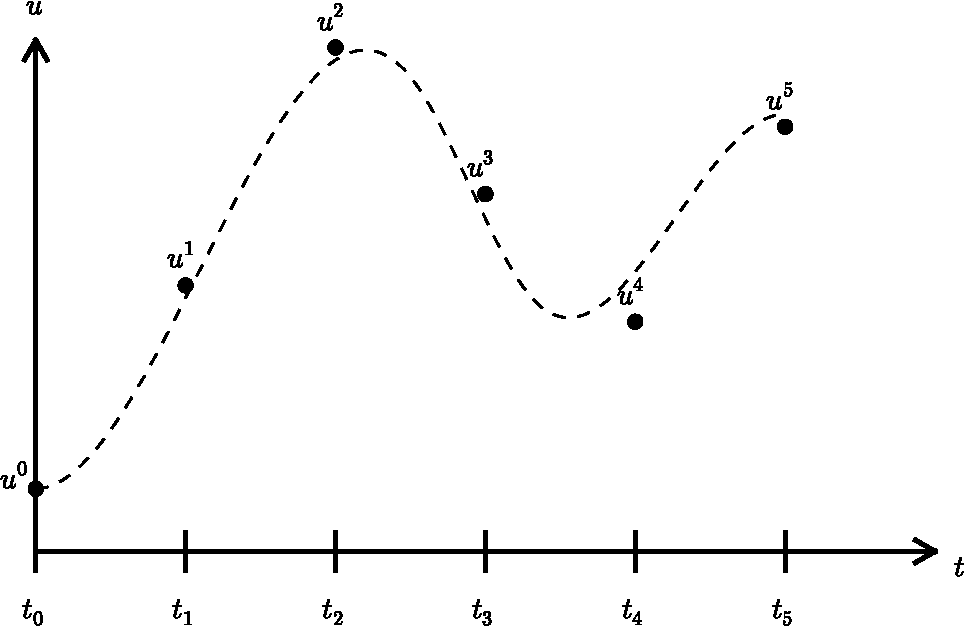
\includegraphics[width=1.0\linewidth]{fig-alg/fdm_u_ue.pdf}}
  \caption{
  Time mesh with discrete solution values at points and a dashed line indicating the true solution. \label{decay:fdu:e}
  }
\end{figure}
%\clearpage % flush figures decay:fdu:e



We say that the numerical approximation, i.e.,
the collection of $u^n$ values for $n=0,\ldots,N_t$,
constitutes a \emph{mesh function}.
A ``normal'' continuous function is a curve defined for all real $t$
values in $[0,T]$, but a mesh function is only defined at discrete
points in time. If you want to compute the mesh function \emph{between} the
mesh points, where it is not defined, an \emph{interpolation method} must be
used. Usually, linear interpolation, i.e., drawing a straight line between
the mesh function values, see Figure~\ref{decay:fdu:e}, suffices.
To compute the solution for some $t\in [t_n, t_{n+1}]$, we use the
linear interpolation formula

\begin{equation}
u(t) \approx u^n + \frac{u^{n+1}-u^n}{t_{n+1}-t_n}(t - t_n)\tp
\end{equation}


\begin{figure}[!ht]  % decay:fdu:ei
  \centerline{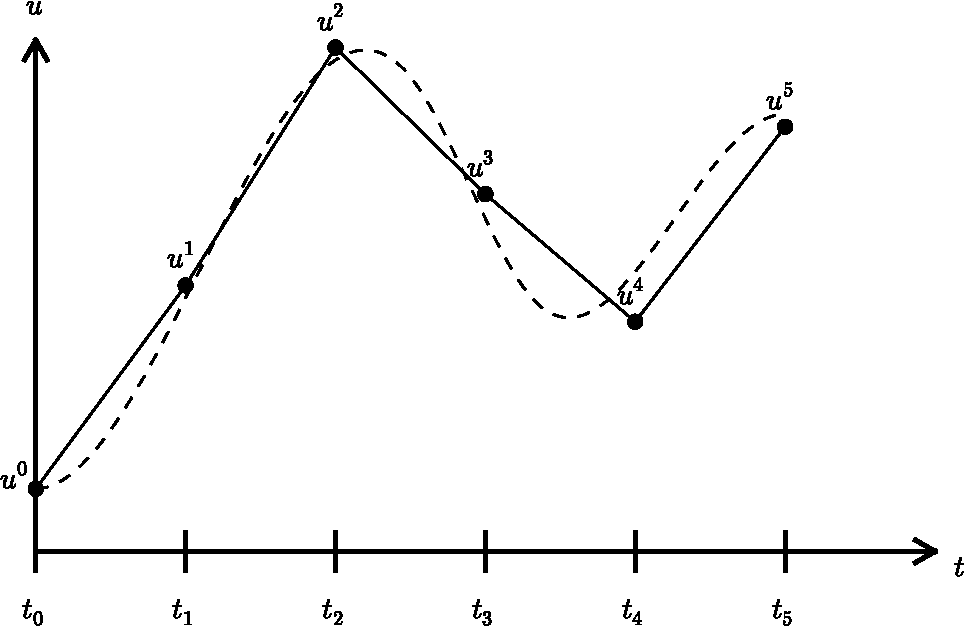
\includegraphics[width=1.0\linewidth]{fig-alg/fdm_u_uei.pdf}}
  \caption{
  Linear interpolation between the discrete solution values (dashed curve is exact solution). \label{decay:fdu:ei}
  }
\end{figure}
%\clearpage % flush figures decay:fdu:ei


\clearpage


\begin{notice_mdfboxadmon}[Notice]
The goal of a numerical solution method for ODEs is
to compute the mesh function by solving a finite set of
\emph{algebraic equations} derived from the original ODE problem.
\end{notice_mdfboxadmon}



\paragraph{Step 2: Fulfilling the equation at discrete time points.}
The ODE is supposed to hold for all $t\in (0,T]$, i.e., at an infinite
number of points. Now we relax that requirement and require that
the ODE is fulfilled at a finite set of discrete points in time.
The mesh points $t_0,t_1,\ldots,t_{N_t}$ are a natural
(but not the only) choice of points.
The original ODE is then reduced to  the following equations:

\begin{equation}
u^{\prime}(t_n) = -au(t_n),\quad n=0,\ldots,N_t,\quad u(0)=I\tp
\label{decay:step2}
\end{equation}
Even though the original ODE is not stated to be valid at $t=0$, it
is valid as close to $t=0$ as we like, and it turns out that it
is useful for construction of numerical methods to have
(\ref{decay:step2}) valid for $n=0$. The next two steps show that we
need (\ref{decay:step2}) for $n=0$.

\index{finite differences}

\paragraph{Step 3: Replacing derivatives by finite differences.}
The next and most essential step of the method is to replace the
derivative $u^{\prime}$ by a finite difference approximation. Let us first
try a \emph{forward} difference approximation (see Figure~\ref{decay:sketch:FE}),

\index{forward difference} \index{finite differences!forward}

\begin{equation}
u^{\prime}(t_n) \approx \frac{u^{n+1}-u^{n}}{t_{n+1}-t_n}\tp
\label{decay:FEdiff}
\end{equation}
The name forward relates to the fact that we use a value forward in
time, $u^{n+1}$, together with the value $u^n$ at the point $t_n$, where
we seek the derivative, to approximate $u^{\prime}(t_n)$.
Inserting this approximation in (\ref{decay:step2}) results in

\begin{equation}
\frac{u^{n+1}-u^{n}}{t_{n+1}-t_n} = -au^{n},\quad n=0,1,\ldots,N_t-1\tp
\label{decay:step3}
\end{equation}
Note that if we want to compute the solution
up to time level $N_t$,
we only need (\ref{decay:step2}) to hold for $n=0,\ldots,N_t-1$ since
(\ref{decay:step3}) for $n=N_t-1$ creates an equation for the final
value $u^{N_t}$.

Also note that we use the approximation symbol $\approx$ in (\ref{decay:FEdiff}),
but not in (\ref{decay:step3}). Instead, we view (\ref{decay:step3}) as
an equation that is not mathematically equivalent to (\ref{decay:FEdiff}),
but represents an approximation to the equation (\ref{decay:FEdiff}).

Equation (\ref{decay:step3})
is the discrete counterpart to the original ODE problem
(\ref{decay:problem}), and often referred to as a \emph{finite difference scheme}
or more generally as the \emph{discrete equations} of the problem.
The fundamental feature of these equations is that they are \emph{algebraic}
and can hence be straightforwardly solved to produce the mesh function, i.e.,
the approximate values of $u$ at
the mesh points: $u^n$, $n=1,2,\ldots,N_t$.


\begin{figure}[!ht]  % decay:sketch:FE
  \centerline{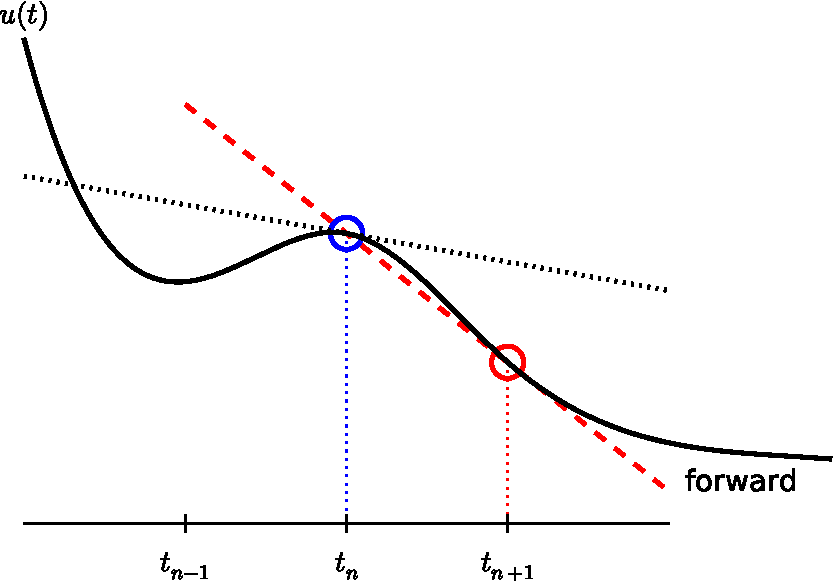
\includegraphics[width=0.8\linewidth]{fig-alg/fd_forward.pdf}}
  \caption{
  Illustration of a forward difference. \label{decay:sketch:FE}
  }
\end{figure}
%\clearpage % flush figures decay:sketch:FE


\index{difference equation}
\index{discrete equation}
\index{algebraic equation}
\index{finite difference scheme}
\index{Forward Euler scheme}

\paragraph{Step 4: Formulating a recursive algorithm.}
The final step is to identify the computational algorithm to be implemented
in a program. The key observation here is to realize that
(\ref{decay:step3}) can be used to compute $u^{n+1}$ if $u^n$ is known.
Starting with $n=0$, $u^0$ is known since $u^0=u(0)=I$, and
(\ref{decay:step3}) gives an equation for $u^1$. Knowing $u^1$,
$u^2$ can be found from (\ref{decay:step3}). In general, $u^n$
in (\ref{decay:step3}) can be assumed known, and then we can easily solve for
the unknown $u^{n+1}$:

\begin{equation}
u^{n+1} = u^n - a(t_{n+1} -t_n)u^n\tp
\label{decay:FE}
\end{equation}
We shall refer to (\ref{decay:FE}) as the Forward Euler (FE) scheme
for our model problem. From a mathematical point of view,
equations of the form (\ref{decay:FE}) are known as
\emph{difference equations} since they express how differences in
the dependent variable, here $u$, evolve with $n$. In our case,
the differences in $u$ are given by $u^{n+1}-u^n = -a(t_{n+1}-t_n)u^n$.
The finite difference method can be viewed as a method for turning
a differential equation into an algebraic difference equation that
can be easily solved by repeated use of a formula like (\ref{decay:FE}).

\paragraph{Interpretation.}
There is a very intuitive interpretation of the FE scheme, illustrated
in the sketch below. We have computed some point values
on the solution curve (small red disks), and the question is how we reason
about the next point. Since we know $u$ and $t$ at the most recently
computed point, the differential equation gives us the \emph{slope} of
the solution curve: $u'=-au$. We can draw this slope as a red line
and continue the solution curve along that slope. As soon as we have
chosen the next point on this line, we have a new $t$ and $u$ value and
can compute a new slope and continue the process.



\vspace{3mm}




\vspace{3mm}





% inline figure
\centerline{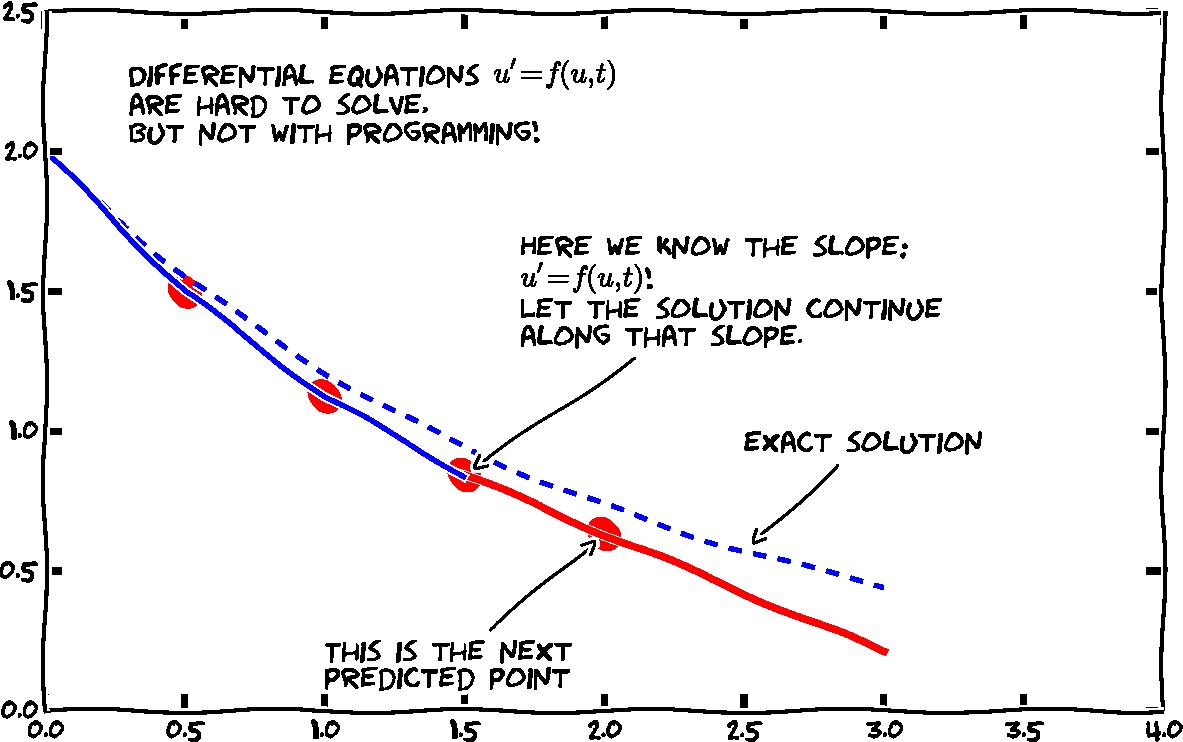
\includegraphics[width=0.8\linewidth]{fig-alg/FE_idea.pdf}}





\vspace{3mm}




\vspace{3mm}



\paragraph{Computing with the recursive formula.}
Mathematical computation with (\ref{decay:FE}) is straightforward:

\begin{align*}
u_0 &= I,\\ 
u_1 & = u^0 - a(t_{1} -t_0)u^0 = I(1-a(t_1-t_0)),\\ 
u_2 & = u^1 - a(t_{2} -t_1)u^1 = I(1-a(t_1-t_0))(1 - a(t_2-t_1)),\\ 
u^3 &= u^2 - a(t_{3} -t_2)u^2 = I(1-a(t_1-t_0))(1 - a(t_2-t_1))(1 - a(t_3-t_2)),
\end{align*}
and so on until we reach $u^{N_t}$.
Very often, $t_{n+1}-t_n$ is constant for all $n$, so we can introduce
the common symbol
$\Delta t = t_{n+1}-t_n$, $n=0,1,\ldots,N_t-1$.
Using a constant mesh spacing $\Delta t$ in the above calculations gives

\begin{align*}
u_0 &= I,\\ 
u_1 & = I(1-a\Delta t),\\ 
u_2 & = I(1-a\Delta t)^2,\\ 
u^3 &= I(1-a\Delta t)^3,\\ 
&\vdots\\ 
u^{N_t} &= I(1-a\Delta t)^{N_t}\tp
\end{align*}
This means that we have found a closed formula for $u^n$, and there is
no need to let a computer generate the sequence $u^1, u^2, u^3, \ldots$.
However, finding such a formula for $u^n$ is possible only for a few very
simple problems, so in general finite difference equations must be
solved on a computer.

As the next sections will show, the scheme (\ref{decay:FE}) is just one
out of many alternative finite difference (and other) methods for
the model problem (\ref{decay:problem}).

\subsection{The Backward Euler scheme}
\label{decay:schemes:BE}

\index{backward difference} \index{finite differences!backward}

There are several choices of difference approximations in step 3 of
the finite difference method as presented in the previous section.
Another alternative is

\begin{equation}
u^{\prime}(t_n) \approx \frac{u^{n}-u^{n-1}}{t_{n}-t_{n-1}}\tp
\label{decay:BEdiff}
\end{equation}
Since this difference is based on going backward in time ($t_{n-1}$)
for information, it is known as a \emph{backward} difference, also called
Backward Euler difference.
Figure~\ref{decay:sketch:BE} explains the idea.


\begin{figure}[!ht]  % decay:sketch:BE
  \centerline{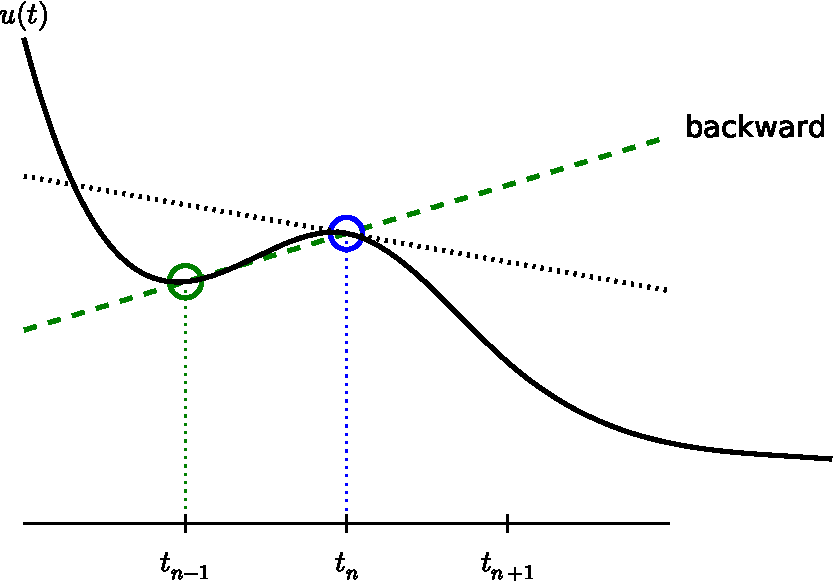
\includegraphics[width=0.8\linewidth]{fig-alg/fd_backward.pdf}}
  \caption{
  Illustration of a backward difference. \label{decay:sketch:BE}
  }
\end{figure}
%\clearpage % flush figures decay:sketch:BE


\index{backward scheme, 1-step}
\index{Backward Euler scheme}

Inserting (\ref{decay:BEdiff}) in (\ref{decay:step2}) yields
the Backward Euler (BE) scheme:

\begin{equation}
\frac{u^{n}-u^{n-1}}{t_{n}-t_{n-1}} = -a u^n,\quad n=1,\ldots,N_t\tp
\label{decay:BE0}
\end{equation}
We assume, as explained under step 4 in Section~\ref{decay:schemes:FE},
that we have computed $u^0, u^1, \ldots, u^{n-1}$ such that
(\ref{decay:BE0}) can be used to compute $u^n$. Note that
(\ref{decay:BE0}) needs $n$ to start at 1 (then it involves $u^0$, but
no $u^{-1}$) and end at $N_t$.

For direct similarity with the formula for the
Forward Euler scheme (\ref{decay:FE})
we replace $n$ by $n+1$ in (\ref{decay:BE0}) and solve for the
unknown value $u^{n+1}$:

\begin{equation}
u^{n+1} = \frac{1}{1+ a(t_{n+1}-t_n)} u^n,\quad n=0,\ldots,N_t-1\tp
\label{decay:BE}
\end{equation}

\subsection{The Crank-Nicolson scheme}
\label{decay:schemes:CN}

\index{Crank-Nicolson scheme}
\index{centered difference} \index{finite differences!centered}


The finite difference approximations
(\ref{decay:FEdiff}) and (\ref{decay:BEdiff}) used to derive the schemes
(\ref{decay:FE}) and (\ref{decay:BE}), respectively,
are both one-sided differences, i.e.,
we collect information either forward or backward in time when approximating
the derivative at a point. Such one-sided differences are
known to be less accurate than central (or midpoint)
differences, where we use information both forward and backward in
time. A natural next step is therefore to construct
a central difference approximation that will yield a more accurate
numerical solution.

The central difference approximation to the derivative is sought at the
point $t_{n+\half}=\half (t_n + t_{n+1})$ (or
$t_{n+\half}=(n+\half)\Delta t$ if the mesh spacing is uniform in time).
The approximation reads

\begin{equation}
u^{\prime}(t_{n+\half}) \approx \frac{u^{n+1}-u^n}{t_{n+1}-t_n}\tp
\label{decay:CNdiff}
\end{equation}
Figure~\ref{decay:sketch:CN} sketches the geometric interpretation of
such a centered difference.
Note that the fraction on the right-hand side is the same as for the
Forward Euler approximation (\ref{decay:FEdiff}) and
the Backward Euler approximation (\ref{decay:BEdiff}) (with
$n$ replaced by $n+1$). The accuracy of this fraction as an approximation
to the derivative of $u$ depends on \emph{where} we seek the derivative:
in the center of the interval $[t_{n},t_{n+1}]$ or at the end points.
We shall later see that it is more accurate at the center point.


\begin{figure}[!ht]  % decay:sketch:CN
  \centerline{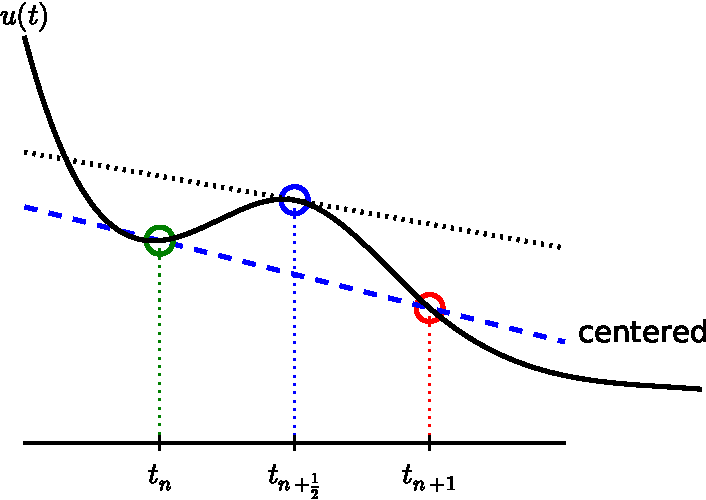
\includegraphics[width=0.8\linewidth]{fig-alg/fd_centered_CN.pdf}}
  \caption{
  Illustration of a centered difference. \label{decay:sketch:CN}
  }
\end{figure}
%\clearpage % flush figures decay:sketch:CN


With the formula (\ref{decay:CNdiff}), where $u^{\prime}$ is evaluated at
$t_{n+\half}$, it is natural to demand the
ODE to be fulfilled at the time points \emph{between} the mesh points:

\begin{equation}
u^{\prime}(t_{n+\half}) = -au(t_{n+\half}),\quad n=0,
\ldots,N_t-1\tp
\label{decay:step2m}
\end{equation}
Using (\ref{decay:CNdiff}) in (\ref{decay:step2m}) results in
the approximate discrete equation

\begin{equation}
\frac{u^{n+1}-u^n}{t_{n+1}-t_n} = -au^{n+\half},\quad n=0,\ldots,N_t-1,
\label{decay:CN0}
\end{equation}
where $u^{n+\half}$ is a short form for the numerical approximation
to $u(t_{n+\half})$.

There is a fundamental problem with the right-hand side of
(\ref{decay:CN0}): we aim to compute $u^n$ for integer $n$, which means
that $u^{n+\half}$ is not a quantity computed by our method. The
quantity must
therefore be
expressed by the quantities that we actually produce, i.e.,
the numerical solution at the
mesh points. One possibility is to approximate $u^{n+\half}$
as an arithmetic mean of the $u$ values at the neighboring mesh points:

\index{averaging!arithmetic}

\begin{equation}
u^{n+\half} \approx \half (u^n + u^{n+1})\tp
\label{decay:uhalfavg}
\end{equation}
Using (\ref{decay:uhalfavg}) in (\ref{decay:CN0}) results in a new
approximate discrete equation

\begin{equation}
\frac{u^{n+1}-u^n}{t_{n+1}-t_n} = -a\half (u^n + u^{n+1})\tp
\label{decay:CN1}
\end{equation}
There are three approximation steps leading to this formula:
1) the ODE is only valid at discrete points (between the mesh points),
2) the derivative is approximated by a finite difference, and 3) the
value of $u$ between mesh points is approximated by an arithmetic mean
value. Despite one more approximation than for the Backward and Forward
Euler schemes, the use of a centered difference leads to a more
accurate method.

To formulate a recursive algorithm,
we assume that $u^n$ is already computed so that $u^{n+1}$ is the
unknown, which we can solve for:

\begin{equation}
u^{n+1} = \frac{1-\half a(t_{n+1}-t_n)}{1 + \half a(t_{n+1}-t_n)}u^n\tp
\label{decay:CN}
\end{equation}
The finite difference scheme (\ref{decay:CN}) is often called
the Crank-Nicolson (CN) scheme or a midpoint or centered scheme.
Note that (\ref{decay:CN}) as well as (\ref{decay:FE}) and (\ref{decay:BE})
apply whether the spacing in the time mesh, $t_{n+1}-t_n$, depends on $n$
or is constant.


\subsection{The unifying $\theta$-rule}
\label{decay:schemes:theta}

\index{weighted average} \index{theta-rule} \index{$\theta$-rule}

The Forward Euler, Backward Euler, and Crank-Nicolson schemes can be
formulated as one scheme with a varying parameter $\theta$:

\begin{equation}
\frac{u^{n+1}-u^{n}}{t_{n+1}-t_n} = -a (\theta u^{n+1} + (1-\theta) u^{n})
\label{decay:th0}
\tp
\end{equation}

Observe that

\begin{itemize}
 \item $\theta =0$ gives the Forward Euler scheme

 \item $\theta =1$ gives the Backward Euler scheme,

 \item $\theta =\half$ gives the Crank-Nicolson scheme.
\end{itemize}

\noindent
We shall later, in Chapter~\ref{decay:analysis}, learn the pros and cons
of the three alternatives.
One may alternatively choose any other value of $\theta$ in $[0,1]$, but
this is not so common since the accuracy and stability of
the scheme do not improve compared
to the values $\theta=0,1,\half$.

As before, $u^n$ is considered known and $u^{n+1}$ unknown, so
we solve for the latter:

\begin{equation}
u^{n+1} = \frac{1 - (1-\theta) a(t_{n+1}-t_n)}{1 + \theta a(t_{n+1}-t_n)}\tp
\label{decay:th}
\end{equation}
This scheme is known as the $\theta$-rule, or alternatively written as
the ``theta-rule''.


\begin{notice_mdfboxadmon}[Derivation.]
We start with replacing $u^{\prime}$ by the fraction

\begin{equation*} \frac{u^{n+1}-u^{n}}{t_{n+1}-t_n},\end{equation*}
in the Forward Euler, Backward Euler,
and Crank-Nicolson schemes. Then we observe that
the difference between the methods concerns which point this
fraction approximates the derivative. Or in other words, at which point we
sample the ODE. So far this has been the
end points or the midpoint of $[t_n,t_{n+1}]$. However, we may choose any point
$\tilde t \in [t_n,t_{n+1}]$.
The difficulty
is that evaluating the right-hand side $-au$ at an arbitrary point
faces the same problem as in
Section~\ref{decay:schemes:CN}: the point value must be expressed
by the discrete $u$ quantities that we compute by the scheme, i.e.,
$u^n$ and $u^{n+1}$. Following the averaging idea from
Section~\ref{decay:schemes:CN},
the value of $u$ at an arbitrary point $\tilde t$ can be
calculated as a \emph{weighted average}, which generalizes the arithmetic mean
$\half u^n + {\half}u^{n+1}$.
The weighted average reads

\begin{equation}
u(\tilde t) \approx \theta u^{n+1} + (1-\theta) u^{n},
\label{decay:thetaavg_u}
\end{equation}
where $\theta\in [0,1]$ is a weighting factor.
We can also express $\tilde t$ as a similar weighted average

\begin{equation}
\tilde t \approx \theta t_{n+1} + (1-\theta) t_{n}\tp
\label{decay:thetaavg_t}
\end{equation}

Let now the ODE hold at the point
$\tilde t\in [t_n,t_{n+1}]$, approximate $u^{\prime}$ by the fraction
$(u^{n+1}-u^{n})/(t_{n+1}-t_n)$, and approximate the right-hand
side $-au$ by the weighted average (\ref{decay:thetaavg_u}).
The result is (\ref{decay:th0}).
\end{notice_mdfboxadmon}



\subsection{Constant time step}

All schemes up to now have been formulated for a general non-uniform
mesh in time: $t_0 < t_1 < \cdots < t_{N_t}$.
Non-uniform meshes are highly relevant
since one can use many points in regions where $u$ varies rapidly, and
fewer points in regions where $u$ is slowly varying. This idea saves
the total number of points and therefore makes it faster to compute the mesh
function $u^n$. Non-uniform meshes are used together with
\emph{adaptive} methods that are able to adjust the time mesh during the
computations (Section~\ref{decay:fd2:adaptiveRK} applies adaptive methods).

\index{time step}

However, a uniformly distributed set of mesh points is not only
convenient, but also
sufficient for many applications. Therefore, it is a very common
choice. We shall
present the finite difference schemes for a uniform point distribution
$t_n=n\Delta t$, where $\Delta t$ is the constant spacing between
the mesh points, also referred to as the \emph{time step}.
The resulting formulas look simpler and are more
well known.


\begin{summary_mdfboxadmon}[Summary of schemes for constant time step]
\begin{alignat}{2}
u^{n+1} &= (1 - a\Delta t )u^n  & \hbox{Forward Euler}
\label{decay:FE:u}\\ 
u^{n+1} &= \frac{1}{1+ a\Delta t} u^n  & \hbox{Backward Euler}
\label{decay:BE:u}\\ 
u^{n+1} &= \frac{1-\half a\Delta t}{1 + \half a\Delta t} u^n & \hbox{Crank-Nicolson}
\label{decay:CN:u}\\ 
u^{n+1} &= \frac{1 - (1-\theta) a\Delta t}{1 + \theta a \Delta t}u^n  & \hbox{The }\theta-\hbox{rule}
\label{decay:th:u}
\end{alignat}
\end{summary_mdfboxadmon}



It is not accidental that we focus on presenting the Forward Euler, Backward
Euler, and Crank-Nicolson schemes. They complement each other with their
different pros and cons, thus providing a useful collection of
solution methods for many differential equation problems.
The unifying notation of the $\theta$-rule makes it convenient to
work with all three methods through just one formula. This is
particularly advantageous in computer implementations since one avoids
if-else tests with formulas that have repetitive elements.


\begin{question_mdfboxadmon}[Test your understanding!]
To check that key concepts are really understood, the reader is
encouraged to apply the explained finite difference techniques
to a slightly different equation. For this purpose, we recommend
you do Exercise~\ref{decay:app:exer:cooling:schemes} now!
\end{question_mdfboxadmon}



\subsection{Mathematical derivation of finite difference formulas}
\label{decay:fd:taylor}

The finite difference formulas for approximating the first derivative
of a function have so far been somewhat justified through graphical
illustrations in Figures~\ref{decay:sketch:FE}, \ref{decay:sketch:BE},
and~\ref{decay:sketch:CN}. The task is to approximate the derivative
at a point of a curve using only two function values. By drawing
a straight line through the points, we have some approximation to
the tangent of the curve and use the slope of this line as
an approximation to the derivative. The slope can be computed by
inspecting the figures.

However, we can alternatively derive the finite difference formulas by
pure mathematics. The key tool for this approach is Taylor series,
or more precisely, approximation of functions by lower-order
Taylor polynomials. Given a function $f(x)$ that is sufficiently
smooth (i.e., $f(x)$ has ``enough derivatives''),
a Taylor polynomial of degree $m$ can be used to approximate the
value of the function $f(x)$ if we know the values of $f$ and its
first $m$ derivatives at some other point $x=a$. The formula for the
Taylor polynomial reads

\begin{align}
f(x) & \approx f(a) + f'(a)(x-a) + \frac{1}{2}f''(a)(x-a)^2 +
\frac{1}{6}f'''(a)(x-a)^3 + \cdots \nonumber\\ 
 &\quad + \frac{1}{m!}\frac{df^{(m)}}{dx^m}(a)(x-a)^m\tp
\end{align}
For a function of time, $f(t)$, related to a mesh with spacing $\Delta t$,
we often need the Taylor polynomial approximation at $f(t_n\pm\Delta t)$
given $f$ and its derivatives at $t=t_n$. Replacing $x$ by $t_n+\Delta t$ and
$a$ by $t_n$ gives

\begin{align}
f(t_n+\Delta t) & \approx f(t_n) + f'(t_n)\Delta t + \frac{1}{2}f''(t_n)
\Delta t^2 +
\frac{1}{6}f'''(t_n)\Delta t^3 + \cdots\nonumber\\ 
&\quad + \frac{1}{m!}\frac{df^{(m)}}{dx^m}(t_n)\Delta t^m\tp
\label{decay:taylor:FE1}
\end{align}

\paragraph{The forward difference.}
We can use (\ref{decay:taylor:FE1}) to find an approximation for
$f'(t_n)$ simply by solving with respect to this quantity:

\begin{align}
f'(t_n) & \approx  \frac{f(t_n+\Delta t) - f(t_n)}{\Delta t}
- \frac{1}{2}f''(t_n)\Delta t -
\frac{1}{6}f'''(t_n)\Delta t^2 + \cdots\nonumber\\ 
&\quad - \frac{1}{m!}\frac{df^{(m)}}{dx^m}(t_n)\Delta t^{m-1}\tp
\label{decay:taylor:FE2}
\end{align}
By letting $m\rightarrow\infty$, this formula is exact, but that is not
so much of practical value. A more interesting observation is that
all the power terms in $\Delta t$ vanish as $\Delta t\rightarrow 0$, i.e.,
the formula

\begin{equation}
f'(t_n) \approx \frac{f(t_n+\Delta t) - f(t_n)}{\Delta t}
\label{decay:taylor:FE3}
\end{equation}
is exact in the limit $\Delta t\rightarrow 0$.

The interesting feature of (\ref{decay:taylor:FE2}) is that we have
a measure of the error in the formula (\ref{decay:taylor:FE3}): the
error is given by the extra terms on the right-hand side of
(\ref{decay:taylor:FE2}). We assume that $\Delta t$ is a small quantity
($\Delta t\ll 1$).
Then $\Delta t^2\ll\Delta t$, $\Delta t^3\ll \Delta t^2$, and so on,
which means that the first term is the dominating term. This first
term reads $-\frac{1}{2}f''(t_n)\Delta t$ and can be taken as a
measure of the error in the Forward Euler formula.

\paragraph{The backward difference.}
To derive the backward difference, we use the Taylor polynomial
approximation at $f(t_n-\Delta t)$:

\begin{align}
f(t_n-\Delta t) &\approx f(t_n) - f'(t_n)\Delta t + \frac{1}{2}f''(t_n)
\Delta t^2 -
\frac{1}{6}f'''(t_n)\Delta t^3+ \cdots\nonumber\\ 
&\quad + \frac{1}{m!}\frac{df^{(m)}}{dx^m}(t_n)\Delta t^m\tp
\label{decay:taylor:BE1}
\end{align}
Solving with respect to $f'(t_n)$ gives

\begin{align}
f'(t_n) &\approx \frac{f(t_n) - f(t_n-\Delta t)}{\Delta t}
+ \frac{1}{2}f''(t_n)\Delta t -
\frac{1}{6}f'''(t_n)\Delta t^2+ \cdots\nonumber\\ 
&\quad - \frac{1}{m!}\frac{df^{(m)}}{dx^m}(t_n)\Delta t^{m-1}\tp
\label{decay:taylor:BE2}
\end{align}
The term $\frac{1}{2}f''(t_n)\Delta t$ can be taken as a simple measure of
the approximation error since it will dominate over the other terms
as $\Delta t\rightarrow 0$.

\paragraph{The centered difference.}
The centered difference approximates the derivative at
$t_n+\frac{1}{2}\Delta t$. Let us write up the Taylor polynomial
approximations to $f(t_n)$ and $f(t_{n+1})$ around $t_n+\frac{1}{2}\Delta t$:

\begin{align}
f(t_n) &\approx f(t_n+\frac{1}{2}\Delta t) -
f'(t_n+\frac{1}{2}\Delta t)\frac{1}{2}\Delta t +
f''(t_n+\frac{1}{2}\Delta t)(\frac{1}{2}\Delta t)^2 -\nonumber\\ 
& \quad f'''(t_n+\frac{1}{2}\Delta t)(\frac{1}{2}\Delta t)^3 + \cdots\\ 
f(t_{n+1}) & \approx f(t_n+\frac{1}{2}\Delta t) +
f'(t_n+\frac{1}{2}\Delta t)\frac{1}{2}\Delta t +
f''(t_n+\frac{1}{2}\Delta t)(\frac{1}{2}\Delta t)^2 +\nonumber\\ 
&\quad f'''(t_n+\frac{1}{2}\Delta t)(\frac{1}{2}\Delta t)^3 + \cdots
\end{align}
Subtracting the first from the second gives

\begin{equation}
f(t_{n+1}) - f(t_n) = f'(t_n+\frac{1}{2}\Delta t)\Delta t
+ 2f'''(t_n+\frac{1}{2}\Delta t)(\frac{1}{2}\Delta t)^3 + \cdots
\label{decay:taylor:CN2}
\end{equation}
Solving with respect to $f'(t_n+\frac{1}{2}\Delta t)$ results
in

\begin{equation}
f'(t_n+\frac{1}{2}\Delta t) \approx \frac{f(t_{n+1}) - f(t_n)}{\Delta t}
- \frac{1}{4}f'''(t_n+\frac{1}{2}\Delta t)\Delta t^2 + c
\cdots
\label{decay:taylor:CN3}
\end{equation}
This time the error measure goes like $\frac{1}{4}f'''\Delta t^2$, i.e.,
it is proportional to $\Delta t^2$ and not only $\Delta t$, which means
that the error goes faster to zero as $\Delta t$ is reduced.
This means that the centered difference formula

\begin{equation}
f'(t_n+\frac{1}{2}\Delta t) \approx \frac{f(t_{n+1}) - f(t_n)}{\Delta t}
\label{decay:taylor:CN4}
\end{equation}
is more accurate than the forward and backward differences for small
$\Delta t$.


\subsection{Compact operator notation for finite differences}
\label{decay:fd:op}

\index{finite difference operator notation} \index{operator notation, finite differences}

Finite difference formulas can be tedious to write and read,
especially for differential equations with many terms and many
derivatives. To save space and help the reader spot
the nature of the difference approximations, we introduce a
compact notation. For a function $u(t)$,
a forward difference approximation is denoted
by the $D_t^+$ operator and written as

\begin{equation}
[D_t^+u]^n = \frac{u^{n+1} - u^{n}}{\Delta t}
\ \left( \approx \frac{d}{dt} u(t_n)\right) \label{fd:D:f}
\tp
\end{equation}
The notation consists of an operator that approximates
differentiation with respect to an independent variable, here $t$.
The operator is built of the symbol $D$, with the
independent variable as subscript
and a superscript denoting the type of difference. The superscript $\,{}^+$
indicates a forward difference.
We place square brackets around the operator and the function it operates
on and specify the mesh point, where the operator is acting, by
a superscript after the closing bracket.

The corresponding operator notation for a centered difference and
a backward difference reads

\begin{equation}
[D_tu]^n = \frac{u^{n+\half} - u^{n-\half}}{\Delta t}
\approx \frac{d}{dt} u(t_n), \label{fd:D:c}
\end{equation}
and
\begin{equation}
[D_t^-u]^n = \frac{u^{n} - u^{n-1}}{\Delta t}
\approx \frac{d}{dt} u(t_n) \label{fd:D:b}
\tp
\end{equation}
Note that the superscript $\,{}^-$ denotes the backward
difference, while no superscript implies a central difference.

An averaging operator is also convenient to have:

\begin{equation}
[\overline{u}^{t}]^n = \half (u^{n-\half} + u^{n+\half} )
\approx u(t_n) \label{fd:mean:a}
\end{equation}
The superscript $t$ indicates that the average is taken along the time
coordinate. The common average $(u^n + u^{n+1})/2$ can now be
expressed as $[\overline{u}^{t}]^{n+\half}$. (When also spatial coordinates
enter the problem, we need the explicit specification of the coordinate
after the bar.)


With our compact notation, the Backward Euler finite difference approximation to $u^{\prime}=-au$ can be written
as

\begin{equation*}
[D_t^-u]^n = -au^n \tp
\end{equation*}
In difference equations we often place the square brackets around
the whole equation, to indicate at which mesh point the equation applies,
since each term must be approximated at the same point:

\begin{equation}
[D_t^- u  = -au]^n \tp
\end{equation}
Similarly, the Forward Euler scheme takes the form

\begin{equation}
[D_t^+ u  = -au]^n,
\end{equation}
while the Crank-Nicolson scheme is written as

\begin{equation}
[D_t u = -a\overline{u}^t]^{n+\half}\tp
\label{fd:compact:ex:CN}
\end{equation}


\begin{question_mdfboxadmon}[Question:]
By use of (\ref{fd:D:c}) and (\ref{fd:mean:a}), are you able to
write out the expressions in (\ref{fd:compact:ex:CN}) to verify that
it is indeed the Crank-Nicolson scheme?
\end{question_mdfboxadmon}




The $\theta$-rule can be specified in operator notation by

\begin{equation}
[\bar D_t u = -a\overline{u}^{t,\theta}]^{n+\theta},\tp
\label{decay:fd1:op:theta}
\end{equation}
We define a new time difference

\begin{equation}
\lbrack\bar D_t u\rbrack^{n+\theta} = \frac{u^{n+1}-u^n}{t^{n+1}-t^n},
\label{decay:fd1:Du:theta}
\end{equation}
to be applied at the time point $t_{n+\theta}\approx\theta t_n + (1-\theta)t_{n+1}$. This weighted average gives rise to the
\emph{weighted averaging operator}

\begin{equation}
\lbrack\overline{u}^{t,\theta}\rbrack^{n+\theta} = (1-\theta)u^{n} + \theta u^{n+1}
\approx u(t_{n+\theta}),
\label{decay:fd1:wmean:a}
\end{equation}
where $\theta\in [0,1]$ as usual. Note that for $\theta =\half$ we recover
the standard centered difference and the standard arithmetic mean.
The idea in (\ref{decay:fd1:op:theta}) is to sample the equation at
$t_{n+\theta}$, use a non-symmetric difference at that
point $[\bar D_t u]^{n+\theta}$, and a weighted (non-symmetric) mean value.

An alternative and perhaps clearer notation is

\[ [D_t u]^{n+\half} = \theta [-au]^{n+1} + (1-\theta)[-au]^{n}\tp \]

Looking at the various examples above and comparing them with the
underlying differential equations, we see immediately which difference
approximations that have been used and at which point they
apply. Therefore, the compact notation effectively communicates the
reasoning behind turning a differential equation into a difference
equation.

% !split

\section{Implementation}
\label{decay:impl1}

We want to make a computer program for solving
\[
u^{\prime}(t) = -au(t),\quad t\in (0,T], \quad u(0)=I,
\]
by finite difference methods. The program should also display
the numerical solution as a curve on the
screen, preferably together with the
exact solution.

\index{directory} \index{folder}

All programs referred to in this section are found in the
\href{{http://tinyurl.com/ofkw6kc/alg}}{\nolinkurl{src/alg}} directory (we use the classical
Unix term \emph{directory} for what many others nowadays call \emph{folder}).

\paragraph{Mathematical problem.}
We want to explore the Forward Euler scheme, the
Backward Euler, and the Crank-Nicolson schemes applied to our model problem.
From an implementational point of view, it is advantageous to
implement the $\theta$-rule
\[
u^{n+1} = \frac{1 - (1-\theta) a\Delta t}{1 + \theta a\Delta t}u^n,
\]
since it can generate the three other schemes by various
choices of $\theta$: $\theta=0$ for Forward Euler, $\theta =1$ for
Backward Euler, and $\theta =1/2$ for Crank-Nicolson.
Given $a$, $u^0=I$, $T$, and $\Delta t$,
our task is to use the $\theta$-rule to
compute $u^1, u^2,\ldots,u^{N_t}$, where $t_{N_t}=N_t\Delta t$, and
$N_t$ the closest integer to $T/\Delta t$.

\subsection{Computer language: Python}

Any programming language can be used to generate the $u^{n+1}$ values from
the formula above. However, in this document we shall mainly make use of
Python. There are several good reasons for this choice:

\begin{itemize}
  \item Python has a very clean, readable syntax (often known as
    "executable pseudo-code").

  \item Python code is very similar to MATLAB code (and MATLAB has a
    particularly widespread use for scientific computing).

  \item Python is a full-fledged, very powerful programming language.

  \item Python is similar to C++, but is much simpler to work with and
    results in more reliable code.

  \item Python has a rich set of modules for scientific computing, and its
    popularity in scientific computing is rapidly growing.

  \item Python was made for being combined with compiled languages
    (C, C++, Fortran), so that existing numerical software can be reused,
    and thereby easing high computational performance with new implementations.

  \item Python has extensive support for administrative tasks
    needed when doing large-scale computational investigations.

  \item Python has extensive support for graphics (visualization,
    user interfaces, web applications).
\end{itemize}

\noindent
Learning Python is easy. Many newcomers to the language will probably
learn enough from the forthcoming examples to perform their own computer
experiments. The examples start with simple Python code and gradually
make use of more powerful constructs as we proceed. Unless it is
inconvenient for the problem at hand, our Python code is made as
close as possible to MATLAB code for easy transition between the two
languages.

The coming programming examples assumes familiarity with
variables, for loops, lists, arrays,
functions, positional arguments, and keyword (named) arguments.
A background in basic MATLAB programming is often enough to understand
Python examples.
Readers who feel the Python examples are too hard to follow will
benefit from reading a tutorial, e.g.,

\begin{itemize}
  \item \href{{http://docs.python.org/2/tutorial/}}{The Official Python Tutorial}

  \item \href{{http://www.tutorialspoint.com/python/}}{Python Tutorial on tutorialspoint.com}

  \item \href{{http://www.learnpython.org/}}{Interactive Python tutorial site}

  \item \href{{http://en.wikibooks.org/wiki/A_Beginner's_Python_Tutorial}}{A Beginner's Python Tutorial}
\end{itemize}

\noindent
The author also has a comprehensive book \cite{Langtangen_2012} that teaches
scientific programming with Python from the ground up.


% bumpy list of refs?

\subsection{Making a solver function}
\label{decay:py1}

We choose to have an array \texttt{u} for storing the $u^n$ values, $n=0,1,\ldots,N_t$.
The algorithmic steps are

\begin{enumerate}
 \item initialize $u^0$

 \item for $t=t_n$, $n=1,2,\ldots,N_t$: compute $u_n$ using
    the $\theta$-rule formula
\end{enumerate}

\noindent
An implementation of a numerical algorithm is often referred to as
a \emph{solver}. We shall now make a solver for our model problem and
realize the solver as a Python function. The function must take
the input data $I$, $a$, $T$, $\Delta t$, and $\theta$ of the problem
as arguments and return the solution as arrays \texttt{u} and \texttt{t} for
$u^n$ and $t^n$, $n=0,\ldots,N_t$. The solver function used as

\begin{cod}{cbg_blue1}\begin{Verbatim}[numbers=none,fontsize=\fontsize{9pt}{9pt},baselinestretch=0.95,xleftmargin=2mm]
u, t = solver(I, a, T, dt, theta)
\end{Verbatim}
\end{cod}
\noindent
One can now easily plot \texttt{u} versus \texttt{t} to visualize the solution.

The function \texttt{solver} may look as follows in Python:

\begin{cod}{cbg_blue1}\begin{Verbatim}[numbers=none,fontsize=\fontsize{9pt}{9pt},baselinestretch=0.95,xleftmargin=2mm]
from numpy import *

def solver(I, a, T, dt, theta):
    """Solve u'=-a*u, u(0)=I, for t in (0,T] with steps of dt."""
    Nt = int(T/dt)            # no of time intervals
    T = Nt*dt                 # adjust T to fit time step dt
    u = zeros(Nt+1)           # array of u[n] values
    t = linspace(0, T, Nt+1)  # time mesh

    u[0] = I                  # assign initial condition
    for n in range(0, Nt):    # n=0,1,...,Nt-1
        u[n+1] = (1 - (1-theta)*a*dt)/(1 + theta*dt*a)*u[n]
    return u, t
\end{Verbatim}
\end{cod}
\noindent

The \texttt{numpy} library contains a lot of functions for array computing. Most
of the function names are similar to what is found
in the alternative scientific computing language MATLAB. Here
we make use of

\begin{itemize}
 \item \texttt{zeros(Nt+1)} for creating an array of size \texttt{Nt+1}
   and initializing the elements to zero

 \item \texttt{linspace(0, T, Nt+1)} for creating an array with \texttt{Nt+1}
   coordinates uniformly distributed between \texttt{0} and \texttt{T}
\end{itemize}

\noindent
The \texttt{for} loop deserves a comment, especially for newcomers to Python.
The construction \texttt{range(0, Nt, s)} generates all integers from \texttt{0} to \texttt{Nt}
in steps of \texttt{s}, \emph{but not including} \texttt{Nt}. Omitting \texttt{s} means \texttt{s=1}.
For example, \texttt{range(0, 6, 3)}
gives \texttt{0} and \texttt{3}, while \texttt{range(0, 6)} generates
the list \texttt{[0, 1, 2, 3, 4, 5]}.
Our loop implies the following assignments to \texttt{u[n+1]}: \texttt{u[1]}, \texttt{u[2]}, ...,
\texttt{u[Nt]}, which is what we want since \texttt{u} has length \texttt{Nt+1}.
The first index in Python arrays or lists is \emph{always} \texttt{0} and the
last is then \texttt{len(u)-1} (the length of an array \texttt{u} is obtained by
\texttt{len(u)} or \texttt{u.size}).

\subsection{Integer division}

The shown implementation of the \texttt{solver} may face problems and
wrong results if \texttt{T}, \texttt{a}, \texttt{dt}, and \texttt{theta} are given as integers
(see Exercises~\ref{decay:exer:intdiv} and~\ref{decay:exer:decay1err}).
The problem is related to \emph{integer division} in Python (as
in Fortran, C, C++, and many other computer languages!): \texttt{1/2} becomes \texttt{0},
while \texttt{1.0/2}, \texttt{1/2.0}, or \texttt{1.0/2.0} all become \texttt{0.5}. So, it is enough
that at least the nominator or the denominator is a real number
(i.e., a \texttt{float} object)
to ensure a correct mathematical division. Inserting
a conversion \texttt{dt = float(dt)}
guarantees that \texttt{dt} is
\texttt{float}.

Another problem with computing $N_t=T/\Delta t$ is that we should
round $N_t$ to the nearest integer. With \texttt{Nt = int(T/dt)} the \texttt{int}
operation picks the largest integer smaller than \texttt{T/dt}. Correct
mathematical rounding as known from school is obtained by
\begin{cod}{cbg_blue1}\begin{Verbatim}[numbers=none,fontsize=\fontsize{9pt}{9pt},baselinestretch=0.95,xleftmargin=2mm]
Nt = int(round(T/dt))
\end{Verbatim}
\end{cod}
\noindent
The complete version of our improved, safer \texttt{solver} function then becomes

\begin{cod}{cbg_blue1}\begin{Verbatim}[numbers=none,fontsize=\fontsize{9pt}{9pt},baselinestretch=0.95,xleftmargin=2mm]
from numpy import *

def solver(I, a, T, dt, theta):
    """Solve u'=-a*u, u(0)=I, for t in (0,T] with steps of dt."""
    dt = float(dt)            # avoid integer division
    Nt = int(round(T/dt))     # no of time intervals
    T = Nt*dt                 # adjust T to fit time step dt
    u = zeros(Nt+1)           # array of u[n] values
    t = linspace(0, T, Nt+1)  # time mesh

    u[0] = I                  # assign initial condition
    for n in range(0, Nt):    # n=0,1,...,Nt-1
        u[n+1] = (1 - (1-theta)*a*dt)/(1 + theta*dt*a)*u[n]
    return u, t
\end{Verbatim}
\end{cod}
\noindent


\subsection{Doc strings}

\index{doc strings}

Right below the header line in the \texttt{solver} function there is a
Python string enclosed in triple double quotes \texttt{"""}.
The purpose of this string object is to document what the function
does and what the arguments are. In this case the necessary
documentation does not span more than one line, but with triple double
quoted strings the text may span several lines:

\begin{cod}{cbg_blue1}\begin{Verbatim}[numbers=none,fontsize=\fontsize{9pt}{9pt},baselinestretch=0.95,xleftmargin=2mm]
def solver(I, a, T, dt, theta):
    """
    Solve

        u'(t) = -a*u(t),

    with initial condition u(0)=I, for t in the time interval
    (0,T]. The time interval is divided into time steps of
    length dt.

    theta=1 corresponds to the Backward Euler scheme, theta=0
    to the Forward Euler scheme, and theta=0.5 to the Crank-
    Nicolson method.
    """
    ...
\end{Verbatim}
\end{cod}
\noindent
Such documentation strings appearing right after the header of
a function are called \emph{doc strings}. There are tools that can automatically
produce nicely formatted documentation by extracting the definition of
functions and the contents of doc strings.

It is strongly recommended to equip any function with a doc string,
unless the purpose of the function
is not obvious. Nevertheless, the forthcoming
text deviates from this rule if the function is explained in the text.


\subsection{Formatting numbers}

Having computed the discrete solution \texttt{u}, it is natural to look at
the numbers:
\begin{cod}{cbg_blue1}\begin{Verbatim}[numbers=none,fontsize=\fontsize{9pt}{9pt},baselinestretch=0.95,xleftmargin=2mm]
# Write out a table of t and u values:
for i in range(len(t)):
    print t[i], u[i]
\end{Verbatim}
\end{cod}
\noindent
This compact \texttt{print} statement unfortunately gives less readable output
because the \texttt{t} and \texttt{u} values are not aligned in nicely formatted columns.
To fix this problem, we recommend to use the \emph{printf format}, supported in most
programming languages inherited from C. Another choice is
Python's recent \emph{format string syntax}. Both kinds of syntax are illustrated
below.

\index{printf format}

Writing \texttt{t[i]} and \texttt{u[i]} in two nicely formatted columns is done like
this with the printf format:

\begin{cod}{cbg_blue1}\begin{Verbatim}[numbers=none,fontsize=\fontsize{9pt}{9pt},baselinestretch=0.95,xleftmargin=2mm]
print 't=%6.3f u=%g' % (t[i], u[i])
\end{Verbatim}
\end{cod}
\noindent
The percentage signs signify "slots" in the text where the variables
listed at the end of the statement are inserted. For each "slot" one
must specify a format for how the variable is going to appear in the
string: \texttt{f} for float (with 6 decimals),
\texttt{s} for pure text, \texttt{d} for an integer, \texttt{g} for a real number
written as compactly as possible, \texttt{9.3E} for scientific notation with
three decimals in a field of width 9 characters (e.g., \texttt{-1.351E-2}),
or \texttt{.2f} for standard decimal notation with two decimals
formatted with minimum width. The printf syntax provides a quick way
of formatting tabular output of numbers with full control of the
layout.

\index{format string syntax (Python)}

The alternative \emph{format string syntax} looks like
\begin{cod}{cbg_blue1}\begin{Verbatim}[numbers=none,fontsize=\fontsize{9pt}{9pt},baselinestretch=0.95,xleftmargin=2mm]
print 't={t:6.3f} u={u:g}'.format(t=t[i], u=u[i])
\end{Verbatim}
\end{cod}
\noindent
As seen, this format allows logical names in the "slots" where
\texttt{t[i]} and \texttt{u[i]} are to be inserted. The "slots" are surrounded
by curly braces, and the logical name is followed by a colon and
then the printf-like specification of how to format real numbers,
integers, or strings.

\subsection{Running the program}

The function and main program shown above must be placed in a file,
say with name \href{{http://tinyurl.com/ofkw6kc/alg/decay_v1.py}}{\nolinkurl{decay_v1.py}} (\texttt{v1} for 1st version of this program).  Make sure you
write the code with a suitable text editor (Gedit, Emacs, Vim,
Notepad++, or similar).  The program is run by executing the file this
way:

\begin{Verbatim}[frame=lines,label=\fbox{{\tiny Terminal}},framesep=2.5mm,framerule=0.7pt,fontsize=\fontsize{9pt}{9pt}]
Terminal> python decay_v1.py
\end{Verbatim}
The text \texttt{Terminal>} just indicates a prompt in a
Unix/Linux or DOS terminal window. After this prompt, which may look
different in your terminal window (depending on the terminal application
and how it is set up), commands like \Verb!python decay_v1.py! can be issued.
These commands are interpreted by the operating system.

We strongly recommend to run Python programs within the IPython shell.
First start IPython by typing \texttt{ipython} in the terminal window.
Inside the IPython shell, our program \Verb!decay_v1.py! is run by the command
\Verb!run decay_v1.py!:

\begin{Verbatim}[frame=lines,label=\fbox{{\tiny Terminal}},framesep=2.5mm,framerule=0.7pt,fontsize=\fontsize{9pt}{9pt}]
Terminal> ipython

In [1]: run decay_v1.py
t= 0.000 u=1
t= 0.800 u=0.384615
t= 1.600 u=0.147929
t= 2.400 u=0.0568958
t= 3.200 u=0.021883
t= 4.000 u=0.00841653
t= 4.800 u=0.00323713
t= 5.600 u=0.00124505
t= 6.400 u=0.000478865
t= 7.200 u=0.000184179
t= 8.000 u=7.0838e-05
\end{Verbatim}

The advantage of running programs in IPython are many, but here
we explicitly mention a few of the most
useful features:

\begin{itemize}
 \item previous commands are easily recalled with the up arrow,

 \item \Verb!%pdb! turns on a debugger so that variables can be examined if the program
   aborts (due to a Python exception),

 \item output of commands are stored in variables,

 \item the computing time spent on a set of statements can be measured with
   the \Verb!%timeit! command,

 \item any operating system command can be executed,

 \item modules can be loaded automatically and other customizations can
   be performed when starting IPython
\end{itemize}

\noindent
Although running programs in IPython is strongly recommended, most
execution examples in the forthcoming text use the standard
Python shell with prompt \texttt{>>>} and run programs through
a typesetting like

\begin{Verbatim}[frame=lines,label=\fbox{{\tiny Terminal}},framesep=2.5mm,framerule=0.7pt,fontsize=\fontsize{9pt}{9pt}]
Terminal> python programname
\end{Verbatim}
The reason is that such typesetting
makes the text more compact in the vertical direction
than showing sessions with IPython syntax.

\label{decay:plotting}
\index{plotting curves}
\index{visualizing curves}

\subsection{Plotting the solution}

Having the \texttt{t} and \texttt{u} arrays, the approximate solution \texttt{u} is visualized
by the intuitive command \texttt{plot(t, u)}:

\begin{cod}{cbg_blue1}\begin{Verbatim}[numbers=none,fontsize=\fontsize{9pt}{9pt},baselinestretch=0.95,xleftmargin=2mm]
from matplotlib.pyplot import *
plot(t, u)
show()
\end{Verbatim}
\end{cod}
\noindent
It will be illustrative to also plot the exact solution
$\uex(t)=Ie^{-at}$ for comparison. We first
need to make a Python function for computing the exact solution:

\begin{cod}{cbg_blue1}\begin{Verbatim}[numbers=none,fontsize=\fontsize{9pt}{9pt},baselinestretch=0.95,xleftmargin=2mm]
def u_exact(t, I, a):
    return I*exp(-a*t)
\end{Verbatim}
\end{cod}
\noindent
It is tempting to just do

\begin{cod}{cbg_blue1}\begin{Verbatim}[numbers=none,fontsize=\fontsize{9pt}{9pt},baselinestretch=0.95,xleftmargin=2mm]
u_e = u_exact(t, I, a)
plot(t, u, t, u_e)
\end{Verbatim}
\end{cod}
\noindent
However, this is not exactly what we want: the \texttt{plot} function draws
straight lines between the discrete points \Verb!(t[n], u_e[n])! while
$\uex(t)$ varies as an exponential function between the mesh points.
The technique for showing the ``exact'' variation of $\uex(t)$ between
the mesh points is to introduce a very fine mesh for $\uex(t)$:

\begin{cod}{cbg_blue1}\begin{Verbatim}[numbers=none,fontsize=\fontsize{9pt}{9pt},baselinestretch=0.95,xleftmargin=2mm]
t_e = linspace(0, T, 1001)      # fine mesh
u_e = u_exact(t_e, I, a)
\end{Verbatim}
\end{cod}
\noindent
We can also plot the curves with different colors and styles, e.g.,

\begin{cod}{cbg_blue1}\begin{Verbatim}[numbers=none,fontsize=\fontsize{9pt}{9pt},baselinestretch=0.95,xleftmargin=2mm]
plot(t_e, u_e, 'b-',         # blue line for u_e
     t,   u,   'r--o')       # red dashes w/circles
\end{Verbatim}
\end{cod}
\noindent

With more than one curve in the plot we need to associate each curve
with a legend. We also want appropriate names on the axes, a title,
and a file containing the plot as an image for inclusion in reports.
The Matplotlib package (\texttt{matplotlib.pyplot}) contains functions for
this purpose. The names of the functions are similar to the plotting
functions known from MATLAB.  A complete function for creating
the comparison plot becomes

\begin{cod}{cbg_blue1}\begin{Verbatim}[numbers=none,fontsize=\fontsize{9pt}{9pt},baselinestretch=0.95,xleftmargin=2mm]
from matplotlib.pyplot import *

def plot_numerical_and_exact(theta, I, a, T, dt):
    """Compare the numerical and exact solution in a plot."""
    u, t = solver(I=I, a=a, T=T, dt=dt, theta=theta)

    t_e = linspace(0, T, 1001)        # fine mesh for u_e
    u_e = u_exact(t_e, I, a)

    plot(t,   u,   'r--o',            # red dashes w/circles
         t_e, u_e, 'b-')              # blue line for exact sol.
    legend(['numerical', 'exact'])
    xlabel('t')
    ylabel('u')
    title('theta=%g, dt=%g' % (theta, dt))
    savefig('plot_%s_%g.png' % (theta, dt))

plot_numerical_and_exact(I=1, a=2, T=8, dt=0.8, theta=1)
show()
\end{Verbatim}
\end{cod}
\noindent
Note that \texttt{savefig} here creates a PNG file whose name includes the
values of $\theta$ and $\Delta t$ so that we can easily distinguish
files from different runs with $\theta$ and $\Delta t$.

The complete code is found in the file
\href{{http://tinyurl.com/ofkw6kc/alg/decay_v2.py}}{\nolinkurl{decay_v2.py}}. The resulting plot
is shown in Figure~\ref{decay:fig:v2}. As seen, there is quite some
discrepancy between the exact and the numerical solution.
Fortunately, the numerical solution approaches the exact one as
$\Delta t$ is reduced.


\begin{figure}[!ht]  % decay:fig:v2
  \centerline{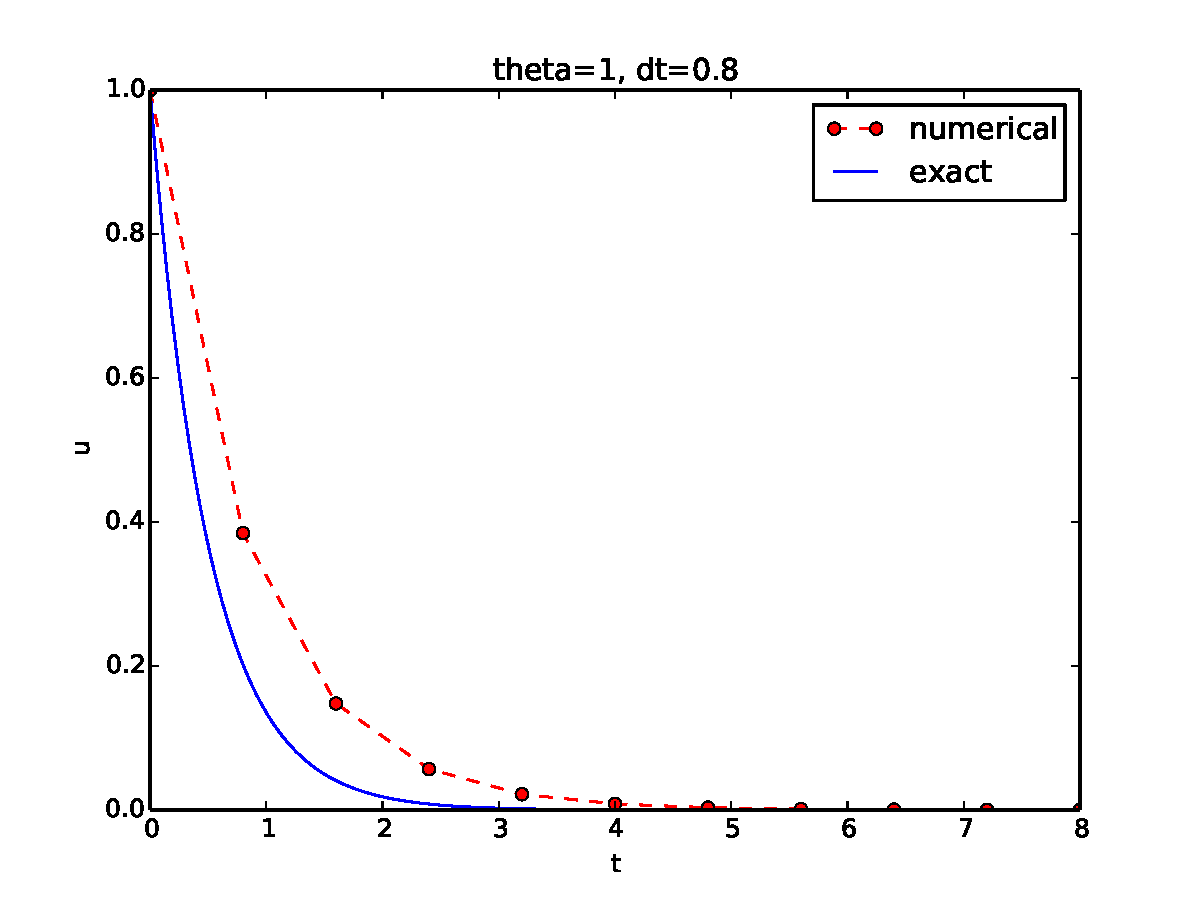
\includegraphics[width=0.8\linewidth]{fig-alg/decay_v2.pdf}}
  \caption{
  Comparison of numerical and exact solution. \label{decay:fig:v2}
  }
\end{figure}
%\clearpage % flush figures decay:fig:v2



\subsection{Verifying the implementation}

It is easy to make mistakes while deriving and implementing numerical
algorithms, so we should never believe in the solution before it has
been thoroughly verified.


\begin{notice_mdfboxadmon}[Verification and validation]
The purpose of \emph{verifying} a program is to bring evidence for the
property that there are no errors in the implementation. A related
term, \emph{validate} (and \emph{validation}),
addresses the question if the ODE model is a good
representation of the phenomena we want to simulate. To remember the
difference between verification and validation, verification is
about \emph{solving the equations right}, while validation is about \emph{solving
the right equations}. We must always perform a verification before
it is meaningful to believe in the computations and perform validation
(which compares the program results with physical experiments or observations).
\end{notice_mdfboxadmon}




The most obvious idea for verification
in our case is to compare the numerical solution with the exact
solution, when that exists. This is, however, not a particularly good
method. The reason is that there will always
be a discrepancy
between these two solutions, due to numerical
approximations, and we cannot precisely quantify the approximation
errors. The open question is therefore whether we have the
mathematically correct
discrepancy or if we have another, maybe small,
discrepancy due to both an approximation error \emph{and} an error in the
implementation. It is thus
impossible to judge whether the program is correct or not by
just looking at the graphs in Figure~\ref{decay:fig:v2}.

To avoid
mixing the unavoidable numerical approximation errors and the
undesired implementation errors, we should try to make tests where
we have some exact
computation of the discrete solution or at least parts of it.
Examples will show how this can be done.

\paragraph{Running a few algorithmic steps by hand.}
The simplest approach to produce a correct non-trivial reference
solution for the discrete solution $u$, is to compute a few steps of
the algorithm by hand. Then we can compare the hand calculations with
numbers produced by the program.

A straightforward approach is to use a calculator and
compute $u^1$, $u^2$, and $u^3$. With $I=0.1$, $\theta=0.8$,
and $\Delta t =0.8$ we get

\[ A\equiv \frac{1 - (1-\theta) a\Delta t}{1 + \theta a \Delta t} = 0.298245614035\]
\begin{align*}
u^1 &= AI=0.0298245614035,\\ 
u^2 &= Au^1= 0.00889504462912,\\ 
u^3 &=Au^2= 0.00265290804728
\end{align*}

Comparison of these manual calculations with the result of the
\texttt{solver} function is carried out in the function

\begin{cod}{cbg_blue1}\begin{Verbatim}[numbers=none,fontsize=\fontsize{9pt}{9pt},baselinestretch=0.95,xleftmargin=2mm]
def test_solver_three_steps():
    """Compare three steps with known manual computations."""
    theta = 0.8; a = 2; I = 0.1; dt = 0.8
    u_by_hand = array([I,
                       0.0298245614035,
                       0.00889504462912,
                       0.00265290804728])

    Nt = 3  # number of time steps
    u, t = solver(I=I, a=a, T=Nt*dt, dt=dt, theta=theta)

    tol = 1E-15  # tolerance for comparing floats
    diff = abs(u - u_by_hand).max()
    success = diff <= tol
    assert success
\end{Verbatim}
\end{cod}
\noindent
The \Verb!test_solver_three_steps! function follows widely used conventions
for \emph{unit testing}. By following such conventions we can at a later
stage easily execute a big test suite for our software. That is, after
a small modification is made to the program, we can by typing just
a short command, run through a large number of tests to check that the
modifications do not break any computations.
The conventions boil down to three rules:

\begin{itemize}
 \item The test function name must start with \Verb!test_! and the function
   cannot take any arguments.

 \item The test must end up in a boolean expression that is \texttt{True} if
   the test was passed and \texttt{False} if it failed.

 \item The function must run \texttt{assert} on the boolean expression, resulting
   in program abortion (due to an \texttt{AssertionError} exception) if
   the test failed.
\end{itemize}

\noindent
The main program can routinely run the verification test prior to
solving the real problem:

\begin{cod}{cbg_blue1}\begin{Verbatim}[numbers=none,fontsize=\fontsize{9pt}{9pt},baselinestretch=0.95,xleftmargin=2mm]
test_solver_three_steps()
plot_numerical_and_exact(I=1, a=2, T=8, dt=0.8, theta=1)
show()
\end{Verbatim}
\end{cod}
\noindent
(Rather than calling \Verb!test_*()! functions explicitly, one will
normally ask a testing framework like nose
or pytest to find and run such functions.)
The complete program including the verification above is
found in the file \href{{http://tinyurl.com/ofkw6kc/alg/decay_v3.py}}{\nolinkurl{decay_v3.py}}.


\subsection{Computing the numerical error as a mesh function}
\label{decay:computing:error}

Now that we have some evidence for a correct implementation, we are in
position to compare the computed $u^n$ values in the \texttt{u} array with
the exact $u$ values at the mesh points, in order to study the error
in the numerical solution.

\index{representative (mesh function)}

A natural way to compare the exact and discrete solutions is to
calculate their difference as a mesh function for the error:

\begin{equation}
e^n = \uex(t_n) - u^n,\quad n=0,1,\ldots,N_t \tp
\end{equation}
We may view the mesh function
$\uex^n = \uex(t_n)$ as a representation of the continuous function $\uex(t)$
defined for all $t\in [0,T]$. In fact,
$\uex^n$ is often called the \emph{representative} of
$\uex$ on the mesh. Then, $e^n = \uex^n - u^n$ is clearly
the difference of two mesh functions.

The error mesh function $e^n$ can be computed by

\begin{cod}{cbg_blue1}\begin{Verbatim}[numbers=none,fontsize=\fontsize{9pt}{9pt},baselinestretch=0.95,xleftmargin=2mm]
u, t = solver(I, a, T, dt, theta)  # Numerical sol.
u_e = u_exact(t, I, a)             # Representative of exact sol.
e = u_e - u
\end{Verbatim}
\end{cod}
\noindent
Note that the mesh functions \texttt{u} and \Verb!u_e! are represented by arrays
and associated with the points in the array \texttt{t}.

\index{array arithmetics} \index{array computing} \index{vectorization}


\begin{notice_mdfboxadmon}[Array arithmetics]
The last statements

\begin{cod}{cbg_blue1}\begin{Verbatim}[numbers=none,fontsize=\fontsize{9pt}{9pt},baselinestretch=0.95,xleftmargin=2mm]
u_e = u_exact(t, I, a)
e = u_e - u
\end{Verbatim}
\end{cod}
\noindent
demonstrate some standard examples of array arithmetics: \texttt{t} is an
array of mesh points that we pass to \Verb!u_exact!. This function
evaluates \texttt{-a*t}, which is a scalar times an array, meaning that
the scalar is multiplied with each array element.
The result is an array, let us call it \texttt{tmp1}. Then
\texttt{exp(tmp1)} means applying the exponential function to each element in
\texttt{tmp1}, giving an array, say \texttt{tmp2}. Finally, \texttt{I*tmp2} is computed
(scalar times array) and \Verb!u_e! refers to this array returned from
\Verb!u_exact!. The expression \Verb!u_e - u! is the difference between
two arrays, resulting in a new array referred to by \texttt{e}.

Replacement of array element computations inside a loop by array
arithmetics is known as \emph{vectorization}.
\end{notice_mdfboxadmon}



\subsection{Computing the norm of the error mesh function}
\label{decay:computing:error:norm}

\index{continuous function norms}
\index{norm!continuous}

Instead of working with the error $e^n$ on the entire mesh, we
often want a single number expressing the size of the error.
This is obtained by taking the norm of the error function.

Let us first define norms of a function $f(t)$
defined for all $t\in [0,T]$.
Three common norms are

\begin{align}
||f||_{L^2} &= \left( \int_0^T f(t)^2 dt\right)^{1/2},
\label{decay:norms:L2}\\ 
||f||_{L^1} &= \int_0^T |f(t)| dt,
\label{decay:norms:L1}\\ 
||f||_{L^\infty} &= \max_{t\in [0,T]}|f(t)|\tp
\label{decay:norms:Linf}
\end{align}
The $L^2$ norm (\ref{decay:norms:L2}) (``L-two norm'')
has nice mathematical properties and
is the most popular norm. It is a generalization
of the well-known Eucledian norm of vectors to functions.
The $L^1$ norm looks simpler and more intuitive, but has less
nice mathematical properties compared to the two other norms, so
it is much less used in computations.
The $L^\infty$ is also called the max norm or the supremum norm
and is widely used. It focuses on a single point with the largest
value of $|f|$, while the other norms measure average behavior of
the function.

In fact, there is a whole family of norms,

\begin{equation}
||f||_{L^p} = \left(\int_0^T f(t)^pdt\right)^{1/p},
\end{equation}
with $p$ real. In particular,
$p=1$ corresponds to the $L^1$ norm above while $p=\infty$ is the
$L^\infty$ norm.

\index{discrete function norms}
\index{mesh function norms}
\index{norm!discrete (mesh function)}

Numerical computations involving mesh functions need corresponding norms.
Given a set of function values, $f^n$, and some associated mesh points, $t_n$,
a numerical integration rule can be used to calculate the $L^2$ and
$L^1$ norms defined above. Imagining that the mesh function is extended
to vary linearly between the mesh points, the Trapezoidal rule is
in fact an exact integration rule. A possible modification of the $L^2$
norm for a mesh function $f^n$ on a uniform mesh with spacing $\Delta t$
is therefore the well-known Trapezoidal integration formula

\[ ||f^n|| = \left(\Delta t\left(\half(f^0)^2 + \half(f^{N_t})^2
+ \sum_{n=1}^{N_t-1} (f^n)^2\right)\right)^{1/2} \]
A common approximation of this expression, motivated by the
convenience of having a simpler formula, is

\[ ||f^n||_{\ell^2} = \left(\Delta t\sum_{n=0}^{N_t} (f^n)^2\right)^{1/2} \tp\]
This is called the discrete $L^2$ norm and denoted by $\ell^2$.
If $||f||_{\ell^2}^2$ (i.e., the square of the norm) is used
instead of the Trapezoidal integration formula,
the error
is $\Delta t((f^0)^2 + (f^{N_t})^2)/2$. This means that the
weights at the end points of the mesh function are perturbed,
but as $\Delta t\rightarrow 0$, the error from this perturbation goes
to zero. As long as we are consistent and
stick to one kind of integration
rule for the norm of a mesh function, the details and accuracy of this
rule is of no concern.

The three discrete norms for a mesh function $f^n$, corresponding to
the $L^2$, $L^1$, and $L^\infty$ norms of $f(t)$ defined above, are
defined by

\begin{align}
||f^n||_{\ell^2} &= \left( \Delta t\sum_{n=0}^{N_t} (f^n)^2\right)^{1/2},
\label{decay:norms:l2}\\ 
||f^n||_{\ell^1} &= \Delta t\sum_{n=0}^{N_t} |f^n|,
\label{decay:norms:l1}\\ 
||f^n||_{\ell^\infty} &= \max_{0\leq n\leq N_t}|f^n|\tp
\label{decay:norms:linf}
\end{align}

Note that the $L^2$, $L^1$, $\ell^2$, and $\ell^1$ norms depend on the
length of the interval of interest (think of $f=1$, then the
norms are proportional to $\sqrt{T}$ or $T$). In some applications it
is convenient to think of a mesh function as just a vector of function
values without any relation to the interval $[0,T]$.
Then one can replace $\Delta t$ by $T/N_t$ and simply drop $T$ (which
is just a common scaling factor in the norm,
independent of the vector of function
values). Moreover, people prefer
to divide by the total length of the vector, $N_t+1$, instead of $N_t$.
This reasoning gives rise to the \emph{vector norms} for a vector
$f=(f_0,\ldots,f_{N})$:

\begin{align}
||f||_2 &= \left( \frac{1}{N+1}\sum_{n=0}^{N} (f_n)^2\right)^{1/2},
\label{decay:norms:vl2}\\ 
||f||_1 &= \frac{1}{N+1}\sum_{n=0}^{N} |f_n|,
\label{decay:norms:vl1}\\ 
||f||_{\ell^\infty} &= \max_{0\leq n\leq N}|f_n|\tp
\label{decay:norms:vlinf}
\end{align}
Here we have used the common vector component notation with subscripts
($f_n$) and $N$ as length. We will mostly work with mesh functions
and use the discrete $\ell^2$
norm (\ref{decay:norms:l2}) or the max norm $\ell^\infty$
(\ref{decay:norms:linf}), but the corresponding vector norms
(\ref{decay:norms:vl2})-(\ref{decay:norms:vlinf}) are also much used
in numerical computations, so it is important to know the different
norms and the relations between them.

\index{error!norms}

A single number that expresses the size of the numerical error
will be taken as $||e^n||_{\ell^2}$ and called $E$:

\begin{equation}
E = \sqrt{\Delta t\sum_{n=0}^{N_t} (e^n)^2}
\label{decay:E}
\end{equation}
The corresponding Python code, using array arithmetics, reads

\begin{cod}{cbg_blue1}\begin{Verbatim}[numbers=none,fontsize=\fontsize{9pt}{9pt},baselinestretch=0.95,xleftmargin=2mm]
E = sqrt(dt*sum(e**2))
\end{Verbatim}
\end{cod}
\noindent
The \texttt{sum} function comes from \texttt{numpy} and computes the sum of the elements
of an array. Also the \texttt{sqrt} function is from \texttt{numpy} and computes the
square root of each element in the array argument.

\index{scalar computing}

\paragraph{Scalar computing.}
Instead of doing array computing \texttt{sqrt(dt*sum(e**2))} we can compute with
one element at a time:
\begin{cod}{cbg_blue1}\begin{Verbatim}[numbers=none,fontsize=\fontsize{9pt}{9pt},baselinestretch=0.95,xleftmargin=2mm]
m = len(u)     # length of u array (alt: u.size)
u_e = zeros(m)
t = 0
for i in range(m):
    u_e[i] = u_exact(t, a, I)
    t = t + dt
e = zeros(m)
for i in range(m):
    e[i] = u_e[i] - u[i]
s = 0  # summation variable
for i in range(m):
    s = s + e[i]**2
error = sqrt(dt*s)
\end{Verbatim}
\end{cod}
\noindent
Such element-wise computing, often called \emph{scalar} computing, takes
more code, is less readable, and runs much slower than what we
can achieve with array computing.





\subsection{Experiments with computing and plotting}


Let us write down a new function that wraps up the computation and all
the plotting statements used for comparing the exact and numerical
solutions. This function can be called with various $\theta$ and
$\Delta t$ values to see how the error depends on the method and mesh
resolution.

\begin{cod}{cbg_blue1}\begin{Verbatim}[numbers=none,fontsize=\fontsize{9pt}{9pt},baselinestretch=0.95,xleftmargin=2mm]
def explore(I, a, T, dt, theta=0.5, makeplot=True):
    """
    Run a case with the solver, compute error measure,
    and plot the numerical and exact solutions (if makeplot=True).
    """
    u, t = solver(I, a, T, dt, theta)    # Numerical solution
    u_e = u_exact(t, I, a)
    e = u_e - u
    E = sqrt(dt*sum(e**2))
    if makeplot:
        figure()                         # create new plot
        t_e = linspace(0, T, 1001)       # fine mesh for u_e
        u_e = u_exact(t_e, I, a)
        plot(t,   u,   'r--o')           # red dashes w/circles
        plot(t_e, u_e, 'b-')             # blue line for exact sol.
        legend(['numerical', 'exact'])
        xlabel('t')
        ylabel('u')
        title('theta=%g, dt=%g' % (theta, dt))
        theta2name = {0: 'FE', 1: 'BE', 0.5: 'CN'}
        savefig('%s_%g.png' % (theta2name[theta], dt))
        savefig('%s_%g.pdf' % (theta2name[theta], dt))
        show()
    return E
\end{Verbatim}
\end{cod}
\noindent

The \texttt{figure()} call is key: without it, a new \texttt{plot} command will
draw the new pair of curves in the same plot window, while we want
the different pairs to appear in separate windows and files.
Calling \texttt{figure()} ensures this.

Instead of including the $\theta$ value in the filename to implicitly
inform about the applied method, the code utilizes a little Python
dictionary that maps each relevant $\theta$ value to a corresponding
acronym for the method name (FE, BE, or CN):

\begin{cod}{cbg_blue1}\begin{Verbatim}[numbers=none,fontsize=\fontsize{9pt}{9pt},baselinestretch=0.95,xleftmargin=2mm]
theta2name = {0: 'FE', 1: 'BE', 0.5: 'CN'}
savefig('%s_%g.png' % (theta2name[theta], dt))
\end{Verbatim}
\end{cod}
\noindent

\index{PNG plot} \index{PDF plot} \index{EPS plot}
\index{viewing graphics files}

The \texttt{explore} function stores the plot in two different image file formats:
PNG and PDF. The PNG format is suitable for
being included in HTML documents, while the PDF format provides
higher quality for {\LaTeX} (i.e., \textsc{pdf}{\LaTeX}) documents.
Frequently used viewers for these
image files on Unix systems are \texttt{gv} (comes with Ghostscript)
for the PDF format and
\texttt{display} (from the ImageMagick software suite) for PNG files:

\begin{Verbatim}[frame=lines,label=\fbox{{\tiny Terminal}},framesep=2.5mm,framerule=0.7pt,fontsize=\fontsize{9pt}{9pt}]
Terminal> gv BE_0.5.pdf
Terminal> display BE_0.5.png
\end{Verbatim}

A main program may run a loop over the three methods (given by
their corresponding $\theta$ values)
and call \texttt{explore} to compute errors and make plots:

\begin{cod}{cbg_blue1}\begin{Verbatim}[numbers=none,fontsize=\fontsize{9pt}{9pt},baselinestretch=0.95,xleftmargin=2mm]
def main(I, a, T, dt_values, theta_values=(0, 0.5, 1)):
    print 'theta   dt       error'  # Column headings in table
    for theta in theta_values:
        for dt in dt_values:
            E = explore(I, a, T, dt, theta, makeplot=True)
            print '%4.1f %6.2f: %12.3E' % (theta, dt, E)

main(I=1, a=2, T=5, dt_values=[0.4, 0.04])
\end{Verbatim}
\end{cod}
\noindent
The file \href{{http://tinyurl.com/ofkw6kc/alg/decay_plot_mpl.py}}{\nolinkurl{decay_plot_mpl.py}}
contains the complete code with the functions above.
Running this program results in

\begin{Verbatim}[frame=lines,label=\fbox{{\tiny Terminal}},framesep=2.5mm,framerule=0.7pt,fontsize=\fontsize{9pt}{9pt}]
Terminal> python decay_plot_mpl.py
theta   dt       error
 0.0   0.40:    2.105E-01
 0.0   0.04:    1.449E-02
 0.5   0.40:    3.362E-02
 0.5   0.04:    1.887E-04
 1.0   0.40:    1.030E-01
 1.0   0.04:    1.382E-02
\end{Verbatim}
We observe that reducing $\Delta t$ by a factor of 10 increases the
accuracy for all three methods. We also see that
the combination of $\theta=0.5$ and a small time step $\Delta t =0.04$
gives a much more accurate solution, and that $\theta=0$ and $\theta=1$
with $\Delta t = 0.4$ result in the least accurate solutions.

Figure~\ref{decay:fig:FE1} demonstrates that the numerical solution
produced by the Forward Euler method with
$\Delta t=0.4$ clearly lies below the exact curve, but that the
accuracy improves considerably by reducing the time step by a factor
of 10.


\begin{figure}[!ht]  % decay:fig:FE1
  \centerline{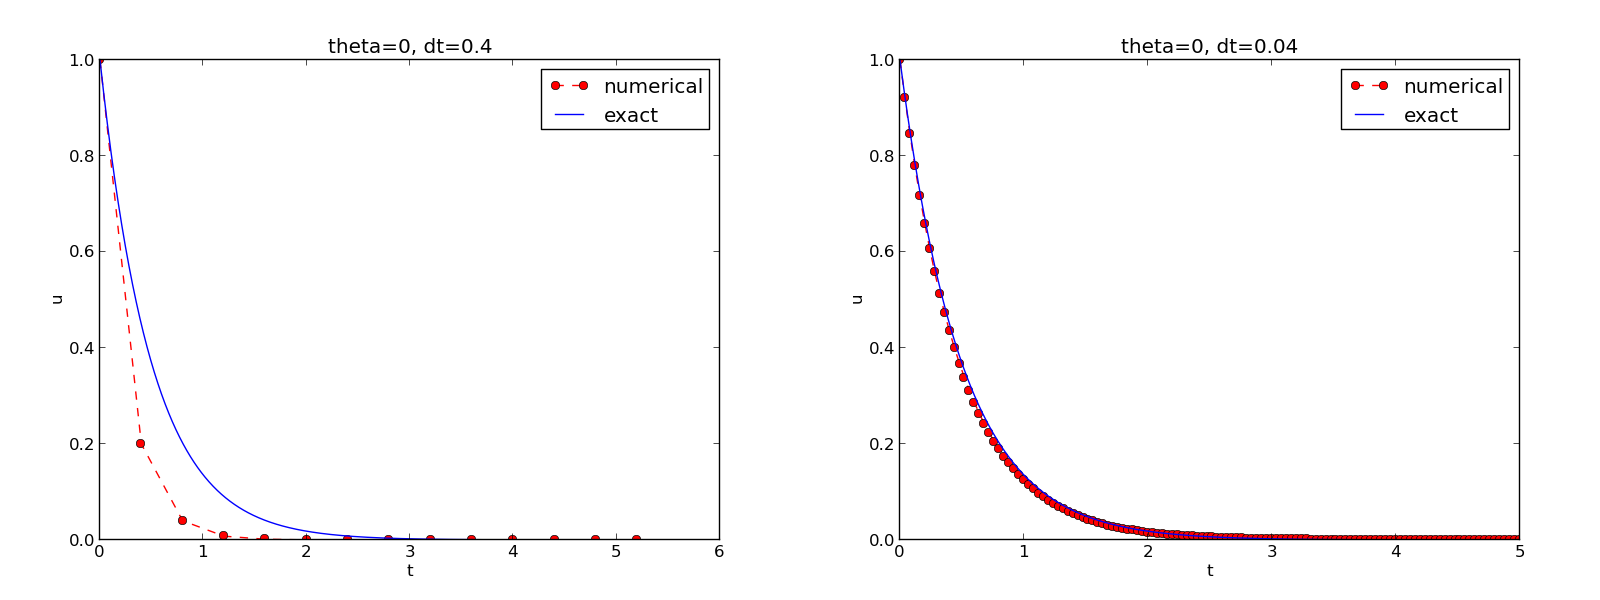
\includegraphics[width=1.1\linewidth]{fig-alg/FE1.png}}
  \caption{
  The Forward Euler scheme for two values of the time step. \label{decay:fig:FE1}
  }
\end{figure}
%\clearpage % flush figures decay:fig:FE1


The behavior of the two other schemes is shown in Figures~\ref{decay:fig:BE1}
and~\ref{decay:fig:CN1}. Crank-Nicolson is obviously the most accurate
scheme from this visual point of view.


\begin{figure}[!ht]  % decay:fig:BE1
  \centerline{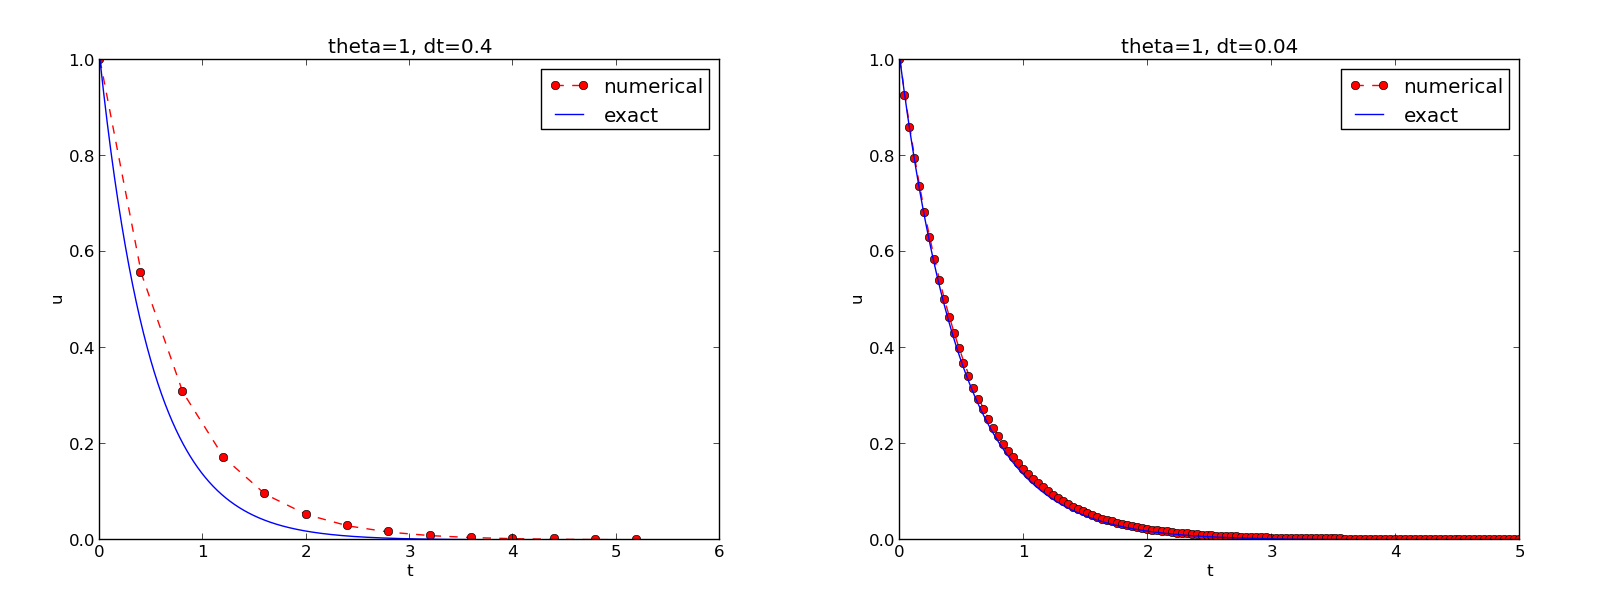
\includegraphics[width=1.1\linewidth]{fig-alg/BE1.png}}
  \caption{
  The Backward Euler scheme for two values of the time step. \label{decay:fig:BE1}
  }
\end{figure}
%\clearpage % flush figures decay:fig:BE1



\begin{figure}[!ht]  % decay:fig:CN1
  \centerline{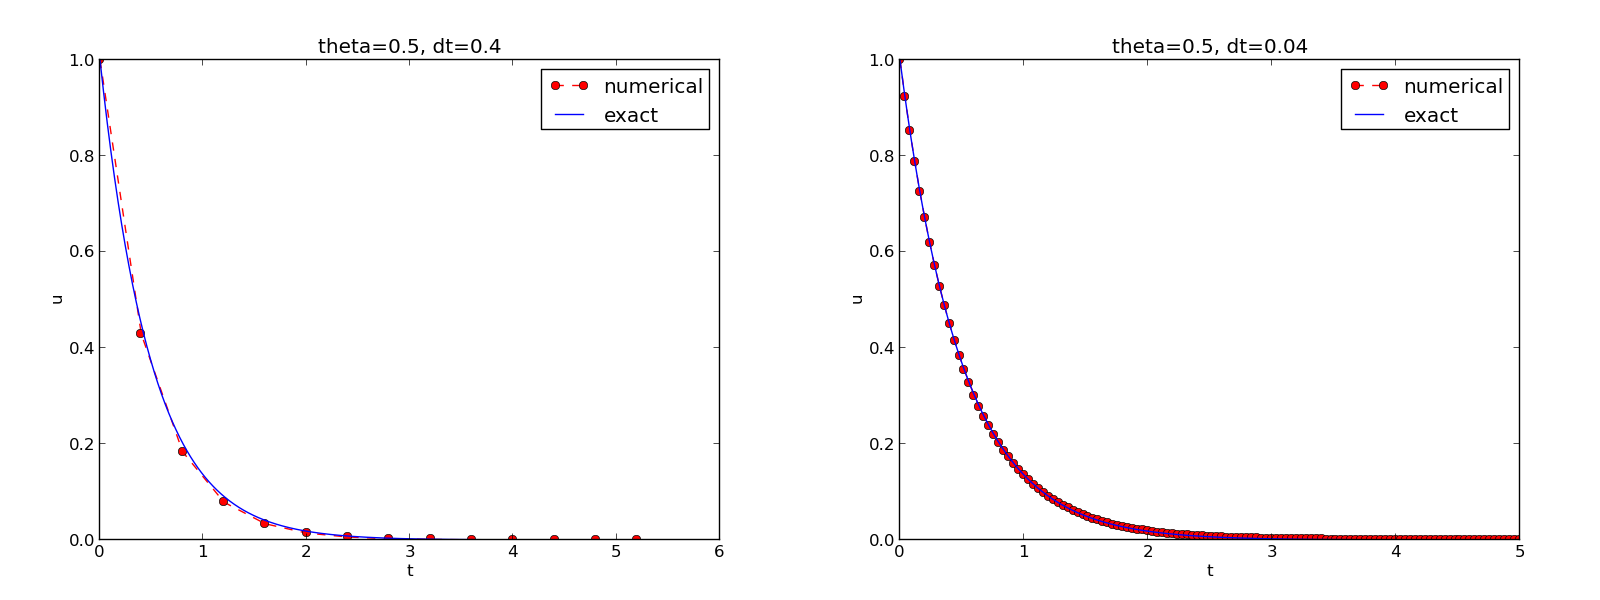
\includegraphics[width=1.1\linewidth]{fig-alg/CN1.png}}
  \caption{
  The Crank-Nicolson scheme for two values of the time step. \label{decay:fig:CN1}
  }
\end{figure}
%\clearpage % flush figures decay:fig:CN1



\index{cropping images}
\index{montage@{\rm\texttt{montage}} program}

\paragraph{Combining plot files.}
Mounting two PNG files beside each other, as done in Figures~\ref{decay:fig:FE1}-\ref{decay:fig:CN1}, is easily carried out by the
\href{{http://www.imagemagick.org/script/montage.php}}{\nolinkurl{montage}} program
from the ImageMagick suite:

\begin{Verbatim}[frame=lines,label=\fbox{{\tiny Terminal}},framesep=2.5mm,framerule=0.7pt,fontsize=\fontsize{9pt}{9pt}]
Terminal> montage -background white -geometry 100% -tile 2x1 \ 
          FE_0.4.png FE_0.04.png FE1.png
Terminal> convert -trim FE1.png FE1.png
\end{Verbatim}
The \texttt{-geometry} argument is used to specify the size of the image. Here,
we preserve the individual sizes of the images. The \texttt{-tile HxV} option
specifies \texttt{H} images in the horizontal direction and \texttt{V} images in
the vertical direction. A series of image files to be combined are then listed,
with the name of the resulting combined image, here \texttt{FE1.png} at the end.
The \texttt{convert -trim} command removes surrounding white areas in the figure
(an operation usually known as \emph{cropping} in image manipulation programs).

\index{pdftk@{\rm\texttt{pdftk}} program}
\index{pdfnup@{\rm\texttt{pdfnup}} program}
\index{pdfcrop@{\rm\texttt{pdfcrop}} program}

For {\LaTeX} reports it is not recommended to use \texttt{montage} and PNG files
as the result has too low resolution. Instead, plots should be made
in the PDF format and combined using the \texttt{pdftk}, \texttt{pdfnup}, and \texttt{pdfcrop} tools
(on Linux/Unix):

\begin{Verbatim}[frame=lines,label=\fbox{{\tiny Terminal}},framesep=2.5mm,framerule=0.7pt,fontsize=\fontsize{9pt}{9pt}]
Terminal> pdftk FE_0.4.png FE_0.04.png output tmp.pdf
Terminal> pdfnup --nup 2x1 --outfile tmp.pdf tmp.pdf
Terminal> pdfcrop tmp.pdf FE1.png  # output in FE1.png
\end{Verbatim}
Here, \texttt{pdftk} combines images into a multi-page PDF file, \texttt{pdfnup}
combines the images in individual pages to a table of images (pages),
and \texttt{pdfcrop} removes white margins in the resulting combined image file.


\paragraph{Plotting with SciTools.}
The \href{{https://github.com/hplgit/scitools}}{SciTools package} provides a
unified plotting interface, called Easyviz, to many different plotting
packages, including Matplotlib, Gnuplot, Grace, MATLAB,
VTK, OpenDX, and VisIt. The syntax is very similar to that of
Matplotlib and MATLAB. In fact, the plotting commands shown above look
the same in SciTool's Easyviz interface, apart from the import
statement, which reads

\begin{cod}{cbg_blue1}\begin{Verbatim}[numbers=none,fontsize=\fontsize{9pt}{9pt},baselinestretch=0.95,xleftmargin=2mm]
from scitools.std import *
\end{Verbatim}
\end{cod}
\noindent
This statement performs a \texttt{from numpy import *} as well as an import
of the most common pieces of the Easyviz (\texttt{scitools.easyviz}) package,
along with some additional numerical functionality.

With Easyviz one can
merge several plotting commands into a single one
using keyword arguments:

\begin{cod}{cbg_blue1}\begin{Verbatim}[numbers=none,fontsize=\fontsize{9pt}{9pt},baselinestretch=0.95,xleftmargin=2mm]
plot(t,   u,   'r--o',           # red dashes w/circles
     t_e, u_e, 'b-',             # blue line for exact sol.
     legend=['numerical', 'exact'],
     xlabel='t',
     ylabel='u',
     title='theta=%g, dt=%g' % (theta, dt),
     savefig='%s_%g.png' % (theta2name[theta], dt),
     show=True)
\end{Verbatim}
\end{cod}
\noindent
The \href{{http://tinyurl.com/ofkw6kc/alg/decay_plot_st.py}}{\nolinkurl{decay_plot_st.py}} file
contains such a demo.

By default, Easyviz employs Matplotlib for plotting, but \href{{http://www.gnuplot.info/}}{Gnuplot} and \href{{http://plasma-gate.weizmann.ac.il/Grace/}}{Grace} are viable alternatives:

\begin{Verbatim}[frame=lines,label=\fbox{{\tiny Terminal}},framesep=2.5mm,framerule=0.7pt,fontsize=\fontsize{9pt}{9pt}]
Terminal> python decay_plot_st.py --SCITOOLS_easyviz_backend gnuplot
Terminal> python decay_plot_st.py --SCITOOLS_easyviz_backend grace
\end{Verbatim}
The actual tool used for creating plots (called \emph{backend})
and numerous other options
can be permanently set in SciTool's configuration file.

All the Gnuplot windows are launched without any need to kill one before
the next one pops up (as is the case with Matplotlib) and one can
press the key 'q' anywhere in a plot window to kill it.
Another advantage of Gnuplot is the automatic choice of sensible
and distinguishable line types in black-and-white PDF and PostScript
files.

For more detailed information on syntax and plotting capabilities,
we refer to the Matplotlib \cite{Matplotlib:doc}
and SciTools \cite{SciTools:doc} documentation.
The hope is that
the programming syntax explained so far suffices for understanding the
basic plotting functionality and being able to look up
the cited technical documentation.


\begin{question_mdfboxadmon}[Test your understanding!]
Exercise~\ref{decay:app:exer:cooling:py} asks you to implement
a solver for a problem that is slightly different from the
one above. You may use the \texttt{solver} and \texttt{explore} functions
explained above as a starting point. Apply the new solver
to solve Exercise~\ref{decay:app:exer:cooling:murder}.
\end{question_mdfboxadmon}





\subsection{Memory-saving implementation}

The computer memory requirements of our implementations so far consist
mainly of the \texttt{u} and \texttt{t} arrays, both of length $N_t+1$.  Also, for
the programs that involve array arithmetics, Python needs memory space
for storing temporary arrays. For example, computing \texttt{I*exp(-a*t)}
requires storing the intermediate result \texttt{a*t} before the preceding
minus sign can be applied. The resulting array is temporarily stored
and provided as input to the \texttt{exp} function.  Regardless of how we
implement simple ODE problems, storage requirements are very modest
and put no restrictions on how we choose our data structures and
algorithms.  Nevertheless, when the presented methods are applied to
three-dimensional PDE problems, memory storage requirements suddenly
become a challenging issue.

Let us briefly elaborate on how large the storage requirements can
quickly be in three-dimensional problems.  The PDE counterpart to our
model problem $u'=-a$ is a diffusion equation $u_t = a\nabla^2 u$
posed on a space-time domain. The discrete representation of this
domain may in 3D be a spatial mesh of $M^3$ points and a time mesh of
$N_t$ points.  In many applications, it is quite typical that $M$ is
at least 100, or even 1000.  Storing all the computed $u$ values, like
we have done in the programs so far, would demand storing arrays of
size up to $M^3N_t$. This would give a factor of $M^3$ larger storage
demands compared to what was required by our ODE programs. Each real
number in the \texttt{u} array requires 8 bytes (b) of storage. With $M=100$
and $N_t=1000$, there is a storage demand of $(10^3)^3\cdot 1000\cdot
8 = 8$ Gb for the solution array.  Fortunately, we can usually get rid
of the $N_t$ factor, resulting in 8 Mb of storage.  Below we explain
how this is done (the technique is almost always applied in
implementations of PDE problems).


Let us critically evaluate how much we really need to store in the
computer's memory for our implementation of the $\theta$ method. To
compute a new $u^{n+1}$, all we need is $u^n$. This implies that the
previous $u^{n-1},u^{n-2},\dots,u^0$ values do not need to be stored,
although this is convenient for plotting and data analysis in the
program.  Instead of the \texttt{u} array we can work with two variables for
real numbers, \texttt{u} and \Verb!u_1!, representing $u^{n+1}$ and $u^n$ in the
algorithm, respectively.  At each time level, we update \texttt{u} from \Verb!u_1!
and then set \Verb!u_1 = u!, so that the computed $u^{n+1}$ value becomes
the "previous" value $u^n$ at the next time level. The downside is
that we cannot plot the solution after the simulation is done since
only the last two numbers are available.  The remedy is to store
computed values in a file and use the file for visualizing the
solution later.

We have implemented this memory saving idea in the file
\href{{http://tinyurl.com/ofkw6kc/alg/decay_memsave.py}}{\nolinkurl{decay_memsave.py}}, which is a
slight modification of \href{{http://tinyurl.com/ofkw6kc/alg/decay_plot_mpl.py}}{\nolinkurl{decay_plot_mpl.py}} program.

The following function demonstrates how we work with the two most
recent values of the unknown:

\begin{cod}{cbg_blue1}\begin{Verbatim}[numbers=none,fontsize=\fontsize{9pt}{9pt},baselinestretch=0.95,xleftmargin=2mm]
def solver_memsave(I, a, T, dt, theta, filename='sol.dat'):
    """
    Solve u'=-a*u, u(0)=I, for t in (0,T] with steps of dt.
    Minimum use of memory. The solution is stored in a file
    (with name filename) for later plotting.
    """
    dt = float(dt)         # avoid integer division
    Nt = int(round(T/dt))  # no of intervals

    outfile = open(filename, 'w')
    # u: time level n+1, u_1: time level n
    t = 0
    u_1 = I
    outfile.write('%.16E  %.16E\n' % (t, u_1))
    for n in range(1, Nt+1):
        u = (1 - (1-theta)*a*dt)/(1 + theta*dt*a)*u_1
        u_1 = u
        t += dt
        outfile.write('%.16E  %.16E\n' % (t, u))
    outfile.close()
    return u, t
\end{Verbatim}
\end{cod}
\noindent
This code snippet also serves as a quick introduction to file writing in Python.
Reading the data in the file into arrays \texttt{t} and \texttt{u} is done by the
function

\begin{cod}{cbg_blue1}\begin{Verbatim}[numbers=none,fontsize=\fontsize{9pt}{9pt},baselinestretch=0.95,xleftmargin=2mm]
def read_file(filename='sol.dat'):
    infile = open(filename, 'r')
    u = [];  t = []
    for line in infile:
        words = line.split()
        if len(words) != 2:
            print 'Found more than two numbers on a line!', words
            sys.exit(1)  # abort
        t.append(float(words[0]))
        u.append(float(words[1]))
    return np.array(t), np.array(u)
\end{Verbatim}
\end{cod}
\noindent

This type of file with numbers in rows and columns is very common, and
\texttt{numpy} has a function \texttt{loadtxt} which loads such tabular data into a
two-dimensional array named by the user. Say the name is \texttt{data}, the
number in row \texttt{i} and column \texttt{j} is then \texttt{data[i,j]}.  The whole
column number \texttt{j} can be extracted by \texttt{data[:,j]}.  A version of
\Verb!read_file! using \texttt{np.loadtxt} reads

\begin{cod}{cbg_blue1}\begin{Verbatim}[numbers=none,fontsize=\fontsize{9pt}{9pt},baselinestretch=0.95,xleftmargin=2mm]
def read_file_numpy(filename='sol.dat'):
    data = np.loadtxt(filename)
    t = data[:,0]
    u = data[:,1]
    return t, u
\end{Verbatim}
\end{cod}
\noindent

The present counterpart to the \texttt{explore} function from
\href{{http://tinyurl.com/ofkw6kc/alg/decay_plot_mpl.py}}{\nolinkurl{decay_plot_mpl.py}} must run
\Verb!solver_memsave! and then load data from file before we can compute
the error measure and make the plot:

\begin{cod}{cbg_blue1}\begin{Verbatim}[numbers=none,fontsize=\fontsize{9pt}{9pt},baselinestretch=0.95,xleftmargin=2mm]
def explore(I, a, T, dt, theta=0.5, makeplot=True):
    filename = 'u.dat'
    u, t = solver_memsave(I, a, T, dt, theta, filename)

    t, u = read_file(filename)
    u_e = u_exact(t, I, a)
    e = u_e - u
    E = sqrt(dt*np.sum(e**2))
    if makeplot:
        figure()
        ...
\end{Verbatim}
\end{cod}
\noindent

Apart from the internal implementation, where $u^n$ values are stored
in a file rather than in an array, \Verb!decay_memsave.py! file works
exactly as the \Verb!decay_plot_mpl.py! file.

% !split
\section{Exercises}



% --- begin exercise ---
\begin{doconceexercise}
\refstepcounter{doconceexercisecounter}

\subsection*{Exercise \thedoconceexercisecounter: Define a mesh function and visualize it}
\addcontentsline{loe}{doconceexercise}{Exercise \thedoconceexercisecounter: Define a mesh function and visualize it}

\label{decay:exer:meshfunc}


\subex{a)}
Write a function \Verb!mesh_function(f, t)! that returns an array with
mesh point values $f(t_0),\ldots,f(t_{N_t})$, where \texttt{f} is a Python
function implementing a mathematical function \texttt{f(t)} and $t_0,\ldots,t_{N_t}$
are mesh points stored in the array \texttt{t}. Use a loop over the mesh
points and compute one mesh function value at the time.


% removed !bsol ... !esol environment (because of the command-line option --without_solutions)

\subex{b)}
Use \Verb!mesh_function! to compute the mesh function corresponding to

\[
f(t) = \left\lbrace
\begin{array}{ll}
e^{-t},& 0\leq t\leq 3,\\ 
e^{-3t}, & 3 < t\leq 4
\end{array}\right.
\]
Choose a mesh $t_n=n\Delta t$ with $\Delta t=0.1$.
Plot the mesh function.


% removed !bsol ... !esol environment (because of the command-line option --without_solutions)



\noindent Filename: \Verb!mesh_function!.

% Closing remarks for this Exercise

\paragraph{Remarks.}
In Section~\ref{decay:computing:error} we show how easy it is to
compute a mesh function by array arithmetics (or array computing).
Using this technique, one could simply implement \Verb!mesh_function(f,t)!
as \texttt{return f(t)}. However, \texttt{f(t)} will not work if there are
if tests involving \texttt{t} inside \texttt{f} as is the case in b). Typically,
\texttt{if t < 3} must have \texttt{t < 3} as a boolean expression, but if \texttt{t} is
array, \texttt{t < 3}, is an \emph{array of boolean values}, which is not legal
as a boolean expression in an if test.
Computing one element
at a time as suggested in a) is a way of out of this problem.

We also remark that the function in b) is the solution of $u^{\prime}=-au$,
$u(0)=1$, for $t\in [0,4]$, where $a=1$ for $t\in [0,3]$ and $a=3$ for
$t\in [3,4]$.


\end{doconceexercise}
% --- end exercise ---




% --- begin exercise ---
\begin{doconceexercise}
\refstepcounter{doconceexercisecounter}

\subsection*{Problem \thedoconceexercisecounter: Differentiate a function}
\addcontentsline{loe}{doconceexercise}{Problem \thedoconceexercisecounter: Differentiate a function}

\label{decay:exer:dudt}

\index{array arithmetics} \index{array computing} \index{vectorization}

Given a mesh function $u^n$ as an array \texttt{u} with $u^n$ values at mesh
points $t_n=n\Delta t$, the discrete derivative can be based on
centered differences:

\begin{equation}
d^n = [D_{2t}u]^n =
\frac{u^{n+1}-u^{n-1}}{2\Delta t},\quad n=1,\ldots,N_t-1\tp
\label{decay:exer:dudt:D2t}
\end{equation}
At the end points we use forward and backward differences:

\[ d^0 = [D_t^+u]^n = \frac{u^{1}-u^{0}}{\Delta t},\]
and

\[ d^{N_t} = [D_t^-u]^n = \frac{u^{N_t}-u^{N_t-1}}{\Delta t}\tp\]


\subex{a)}
Write a function
\texttt{differentiate(u, dt)} that returns the discrete derivative $d^n$ of the
mesh function $u^n$. The parameter \texttt{dt} reflects the
mesh spacing $\Delta t$. Write a corresponding test function
\Verb!test_differentiate()! for verifying the implementation.

% --- begin hint in exercise ---

\paragraph{Hint.}
The three differentiation formulas are
exact for quadratic polynomials. Use this property to verify the program.

% --- end hint in exercise ---


% removed !bsol ... !esol environment (because of the command-line option --without_solutions)

\subex{b)}
A standard implementation of the formula (\ref{decay:exer:dudt:D2t}) is to
have a loop over $i$. For large $N_t$, such loop may run slowly in
Python. A technique for speeding up the computations, called vectorization
or array computing,
replaces the loop by array operations. To see how this can be done in
the present mathematical problem, we
define two arrays

\begin{align*}
u^+ &= (u^2,u^3,\ldots,u^{N_t}),
u^- &= (u^0,u^1,\ldots,u^{N_t-2})\tp
\end{align*}
The formula (\ref{decay:exer:dudt:D2t}) can now be expressed as

\[ (d^1,d^2,\ldots,d^{N_t-1}) = \frac{1}{2\Delta t}(u^+ - u^-)\tp\]
The corresponding Python code reads

\begin{cod}{cbg_blue1}\begin{Verbatim}[numbers=none,fontsize=\fontsize{9pt}{9pt},baselinestretch=0.95,xleftmargin=2mm]
d[1:-1] = (u[2:] - u[0:-2])/(2*dt)
# or
d[1:N_t] = (u[2:N_t+1] - u[0:N_t-1])/(2*dt)
\end{Verbatim}
\end{cod}
\noindent
Recall that an array slice \texttt{u[1:-1]} contains the elements in \texttt{u} starting
with index 1 and going all indices up to, but not including, the last one
(\texttt{-1}).

Use the ideas above to implement a vectorized version of the
\texttt{differentiate} function without loops. Make a corresponding
test function that compares the result with that of
\texttt{differentiate}.


% removed !bsol ... !esol environment (because of the command-line option --without_solutions)

\noindent Filename: \texttt{differentiate}.

\end{doconceexercise}
% --- end exercise ---




% --- begin exercise ---
\begin{doconceexercise}
\refstepcounter{doconceexercisecounter}

\subsection*{Problem \thedoconceexercisecounter: Experiment with divisions}
\addcontentsline{loe}{doconceexercise}{Problem \thedoconceexercisecounter: Experiment with divisions}

\label{decay:exer:intdiv}

Explain what happens in the following computations, where
some are mathematically unexpected:

\begin{cod}{cbg_blue1}\begin{Verbatim}[numbers=none,fontsize=\fontsize{9pt}{9pt},baselinestretch=0.95,xleftmargin=2mm]
>>> dt = 3
>>> T = 8
>>> Nt = T/dt
>>> Nt
2
>>> theta = 1; a = 1
>>> (1 - (1-theta)*a*dt)/(1 + theta*dt*a)
0
\end{Verbatim}
\end{cod}
\noindent


% removed !bsol ... !esol environment (because of the command-line option --without_solutions)
\noindent Filename: \texttt{pyproblems}.

\end{doconceexercise}
% --- end exercise ---




% --- begin exercise ---
\begin{doconceexercise}
\refstepcounter{doconceexercisecounter}

\subsection*{Problem \thedoconceexercisecounter: Experiment with wrong computations}
\addcontentsline{loe}{doconceexercise}{Problem \thedoconceexercisecounter: Experiment with wrong computations}

\label{decay:exer:decay1err}

Consider the \texttt{solver} function in the \href{{http://tinyurl.com/ofkw6kc/alg/decay_v1.py}}{\nolinkurl{decay_v1.py}} file
and the following call:

\begin{cod}{cbg_blue1}\begin{Verbatim}[numbers=none,fontsize=\fontsize{9pt}{9pt},baselinestretch=0.95,xleftmargin=2mm]
u, t = solver(I=1, a=1, T=7, dt=2, theta=1)
\end{Verbatim}
\end{cod}
\noindent
The output becomes

\begin{cod}{cbg_blue1}\begin{Verbatim}[numbers=none,fontsize=\fontsize{9pt}{9pt},baselinestretch=0.95,xleftmargin=2mm]
t= 0.000 u=1
t= 2.000 u=0
t= 4.000 u=0
t= 6.000 u=0
\end{Verbatim}
\end{cod}
\noindent
Print out the result of all intermediate computations and use
\texttt{type(v)} to see the object type of the result stored in some variable \texttt{v}.
Examine the intermediate calculations and explain
why \texttt{u} is wrong and why we compute up to $t=6$ only even though we
specified $T=7$.


% removed !bsol ... !esol environment (because of the command-line option --without_solutions)
\noindent Filename: \Verb!decay_v1_err!.

\end{doconceexercise}
% --- end exercise ---




% --- begin exercise ---
\begin{doconceexercise}
\refstepcounter{doconceexercisecounter}

\subsection*{Problem \thedoconceexercisecounter: Plot the error function}
\addcontentsline{loe}{doconceexercise}{Problem \thedoconceexercisecounter: Plot the error function}

\label{decay:exer:plot:error}

Solve the problem $u'=-au$, $u(0)=I$, using the Forward Euler, Backward
Euler, and Crank-Nicolson schemes. For each scheme, plot the error mesh
function $e^n = \uex(t_n)-u^n$ for $\Delta t$, $\frac{1}{4}\Delta t$, and
$\frac{1}{8}\Delta t$, where $\uex$ is the exact solution of the ODE and
$u^n$ is the numerical solution at mesh point $t_n$.

% --- begin hint in exercise ---

\paragraph{Hint.}
Modify the \href{{http://tinyurl.com/ofkw6kc/alg/decay_plot_mpl.py}}{\nolinkurl{decay_plot_mpl.py}} code.

% --- end hint in exercise ---


% removed !bsol ... !esol environment (because of the command-line option --without_solutions)
\noindent Filename: \Verb!decay_plot_error!.

\end{doconceexercise}
% --- end exercise ---




% --- begin exercise ---
\begin{doconceexercise}
\refstepcounter{doconceexercisecounter}

\subsection*{Problem \thedoconceexercisecounter: Change formatting of numbers and debug}
\addcontentsline{loe}{doconceexercise}{Problem \thedoconceexercisecounter: Change formatting of numbers and debug}

\label{decay:exer:inexact:output}

The \href{{http://tinyurl.com/ofkw6kc/alg/decay_memsave.py}}{\nolinkurl{decay_memsave.py}} program
writes the time values and solution values to a file which looks
like
\begin{cod}{cbg_blue1}\begin{Verbatim}[numbers=none,fontsize=\fontsize{9pt}{9pt},baselinestretch=0.95,xleftmargin=2mm]
0.0000000000000000E+00  1.0000000000000000E+00
2.0000000000000001E-01  8.3333333333333337E-01
4.0000000000000002E-01  6.9444444444444453E-01
6.0000000000000009E-01  5.7870370370370383E-01
8.0000000000000004E-01  4.8225308641975323E-01
1.0000000000000000E+00  4.0187757201646102E-01
1.2000000000000000E+00  3.3489797668038418E-01
1.3999999999999999E+00  2.7908164723365347E-01
\end{Verbatim}
\end{cod}
\noindent
Modify the file output such that it looks like
\begin{cod}{cbg_blue1}\begin{Verbatim}[numbers=none,fontsize=\fontsize{9pt}{9pt},baselinestretch=0.95,xleftmargin=2mm]
0.000  1.00000
0.200  0.83333
0.400  0.69444
0.600  0.57870
0.800  0.48225
1.000  0.40188
1.200  0.33490
1.400  0.27908
\end{Verbatim}
\end{cod}
\noindent
If you have just modified the formatting of numbers in the file,
running the modified program
\begin{Verbatim}[frame=lines,label=\fbox{{\tiny Terminal}},framesep=2.5mm,framerule=0.7pt,fontsize=\fontsize{9pt}{9pt}]
Terminal> python decay_memsave_v2.py --T 10 --theta 1 \ 
          --dt 0.2 --makeplot
\end{Verbatim}
leads to printing of the message \Verb?Bug in the implementation!? in the
terminal window. Why?


% removed !bsol ... !esol environment (because of the command-line option --without_solutions)
\noindent Filename: \Verb!decay_memsave_v2!.

\end{doconceexercise}
% --- end exercise ---


% !split
\chapter{Analysis}
\label{decay:analysis}



We address the ODE for exponential decay,
\begin{equation}
u'(t) = -au(t),\quad u(0)=I,
\end{equation}
where $a$ and $I$ are given constants. This problem is solved
by the $\theta$-rule finite difference scheme, resulting in
the recursive equations
\begin{equation}
u^{n+1} = \frac{1 - (1-\theta) a\Delta t}{1 + \theta a\Delta t}u^n
\label{decay:analysis:scheme}
\end{equation}
for the numerical solution $u^{n+1}$, which approximates the exact
solution $\uex$ at time point $t_{n+1}$. For constant mesh spacing,
which we assume here, $t_{n+1}=(n+1)\Delta t$.

The example programs associated with this chapter are found in
the directory \href{{http://tinyurl.com/ofkw6kc/analysis}}{\nolinkurl{src/analysis}}.

\section{Experimental investigations}

We first perform a series of numerical explorations to see how the
methods behave as we change the parameters $I$, $a$, and $\Delta t$
in the problem.

\subsection{Discouraging numerical solutions}

Choosing $I=1$, $a=2$, and running experiments with $\theta =1,0.5, 0$
for $\Delta t=1.25, 0.75, 0.5, 0.1$, gives the results in
Figures~\ref{decay:analysis:BE4c}, \ref{decay:analysis:CN4c}, and~\ref{decay:analysis:FE4c}.


\begin{figure}[!ht]  % decay:analysis:BE4c
  \centerline{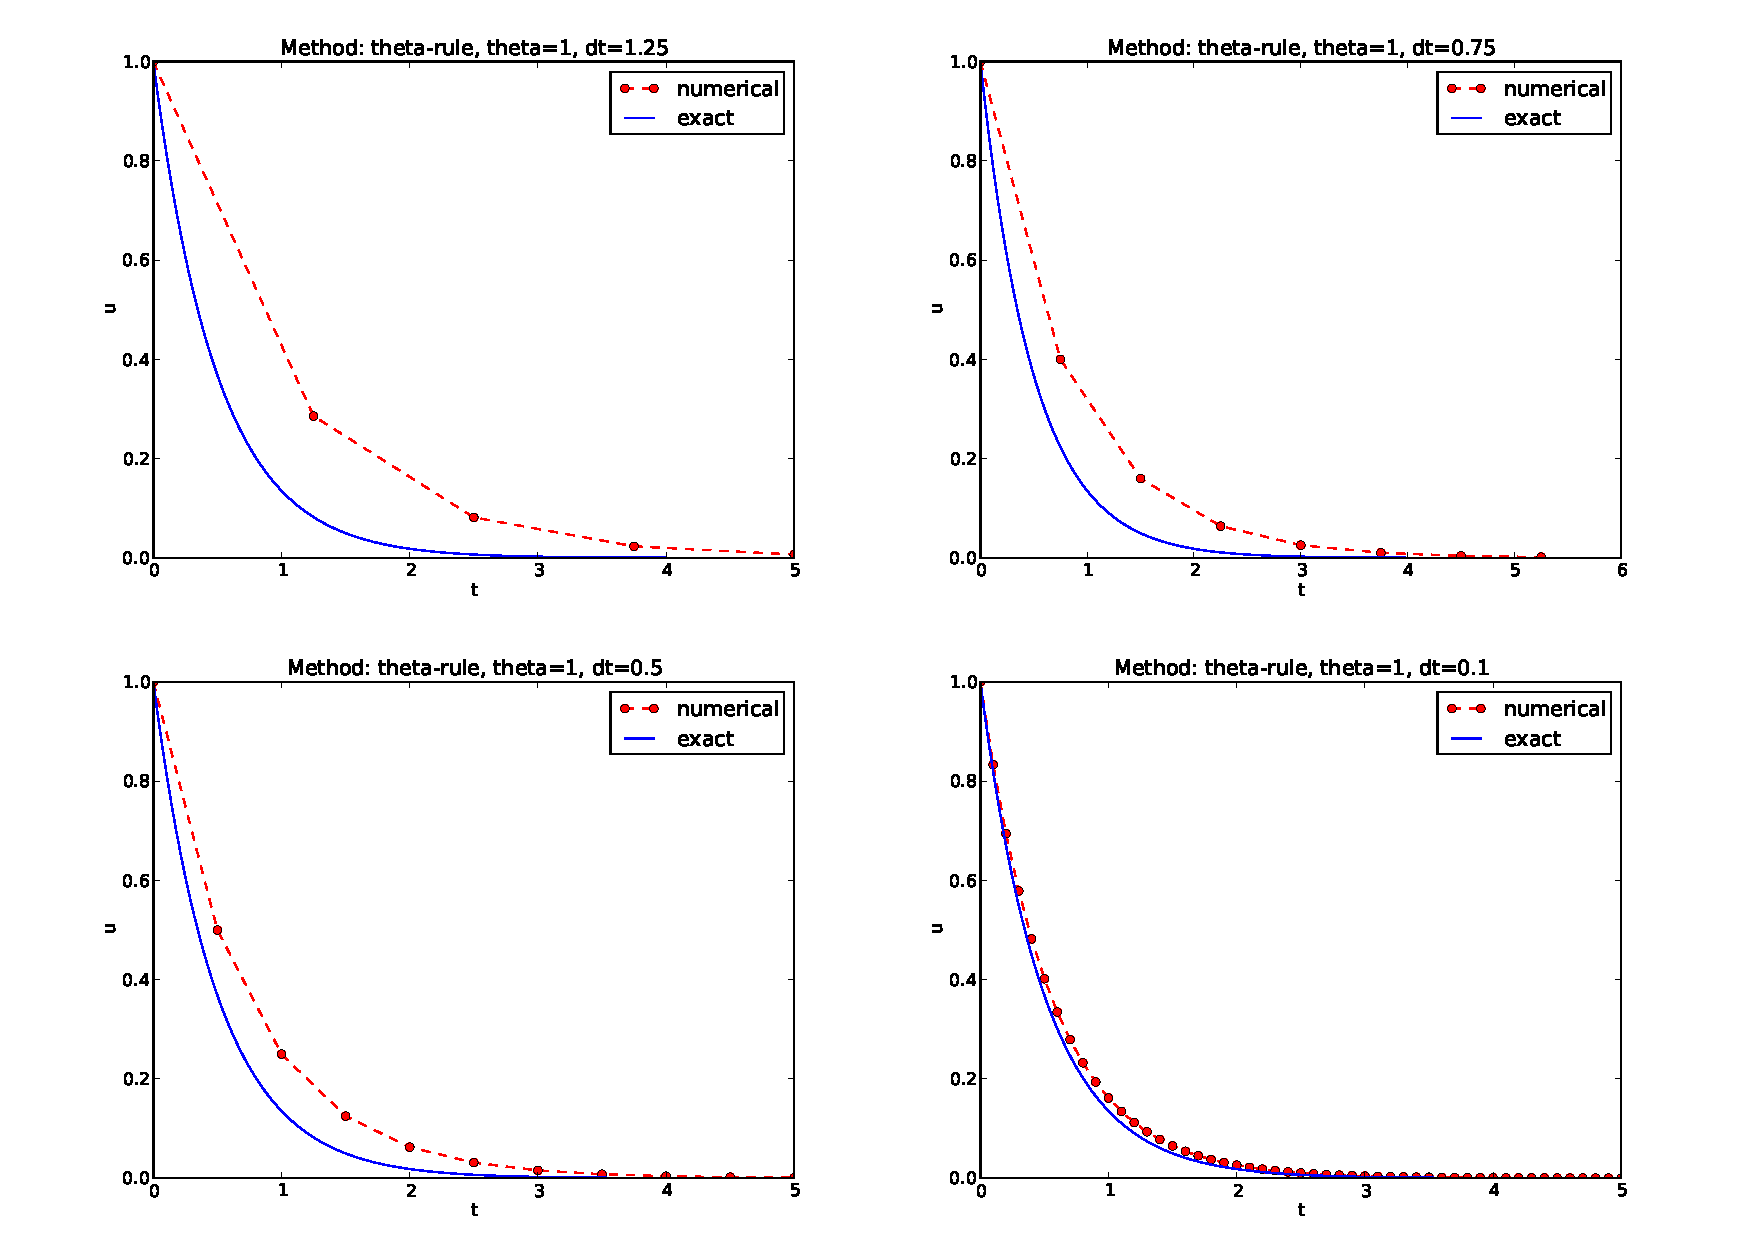
\includegraphics[width=1.1\linewidth]{fig-analysis/BE4c.pdf}}
  \caption{
  Backward Euler. \label{decay:analysis:BE4c}
  }
\end{figure}
%\clearpage % flush figures decay:analysis:BE4c



\begin{figure}[!ht]  % decay:analysis:CN4c
  \centerline{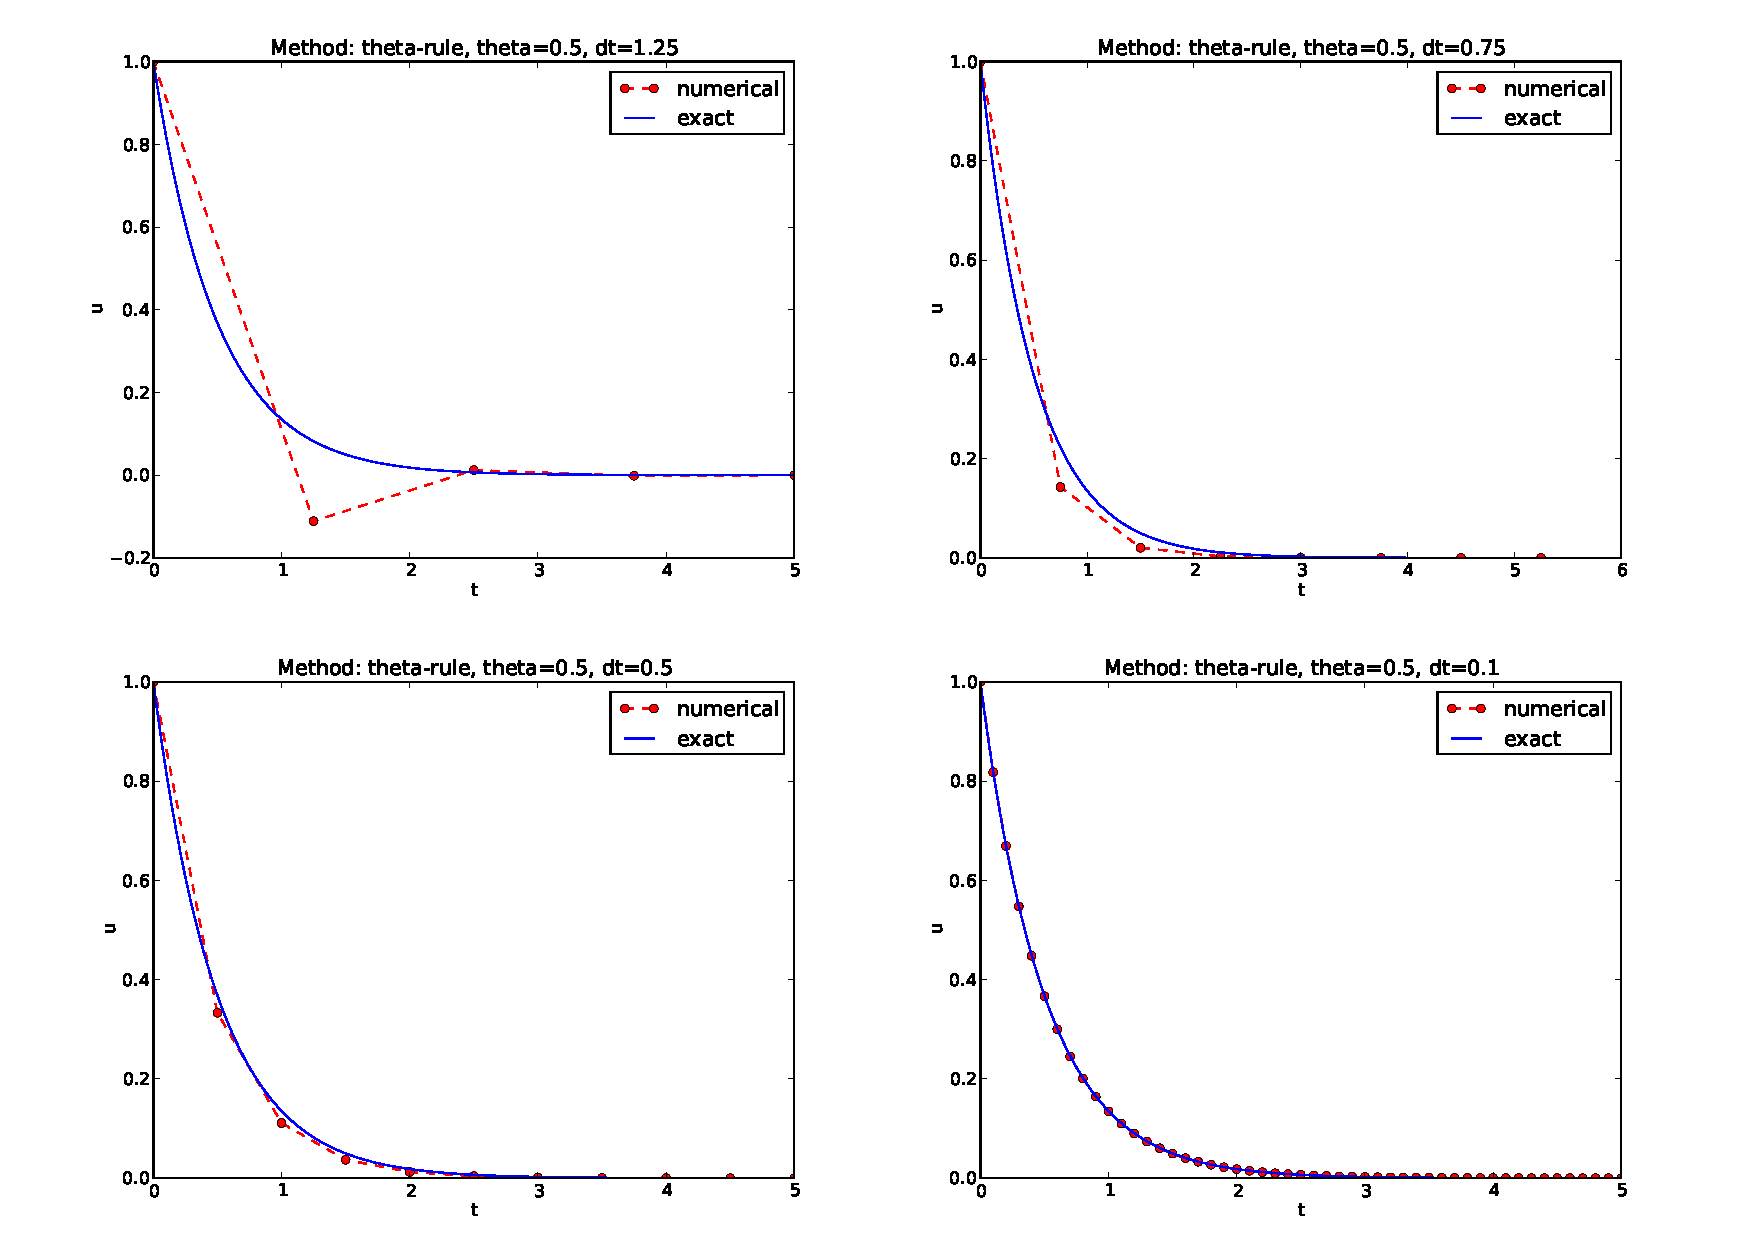
\includegraphics[width=1.1\linewidth]{fig-analysis/CN4c.pdf}}
  \caption{
  Crank-Nicolson. \label{decay:analysis:CN4c}
  }
\end{figure}
%\clearpage % flush figures decay:analysis:CN4c



\begin{figure}[!ht]  % decay:analysis:FE4c
  \centerline{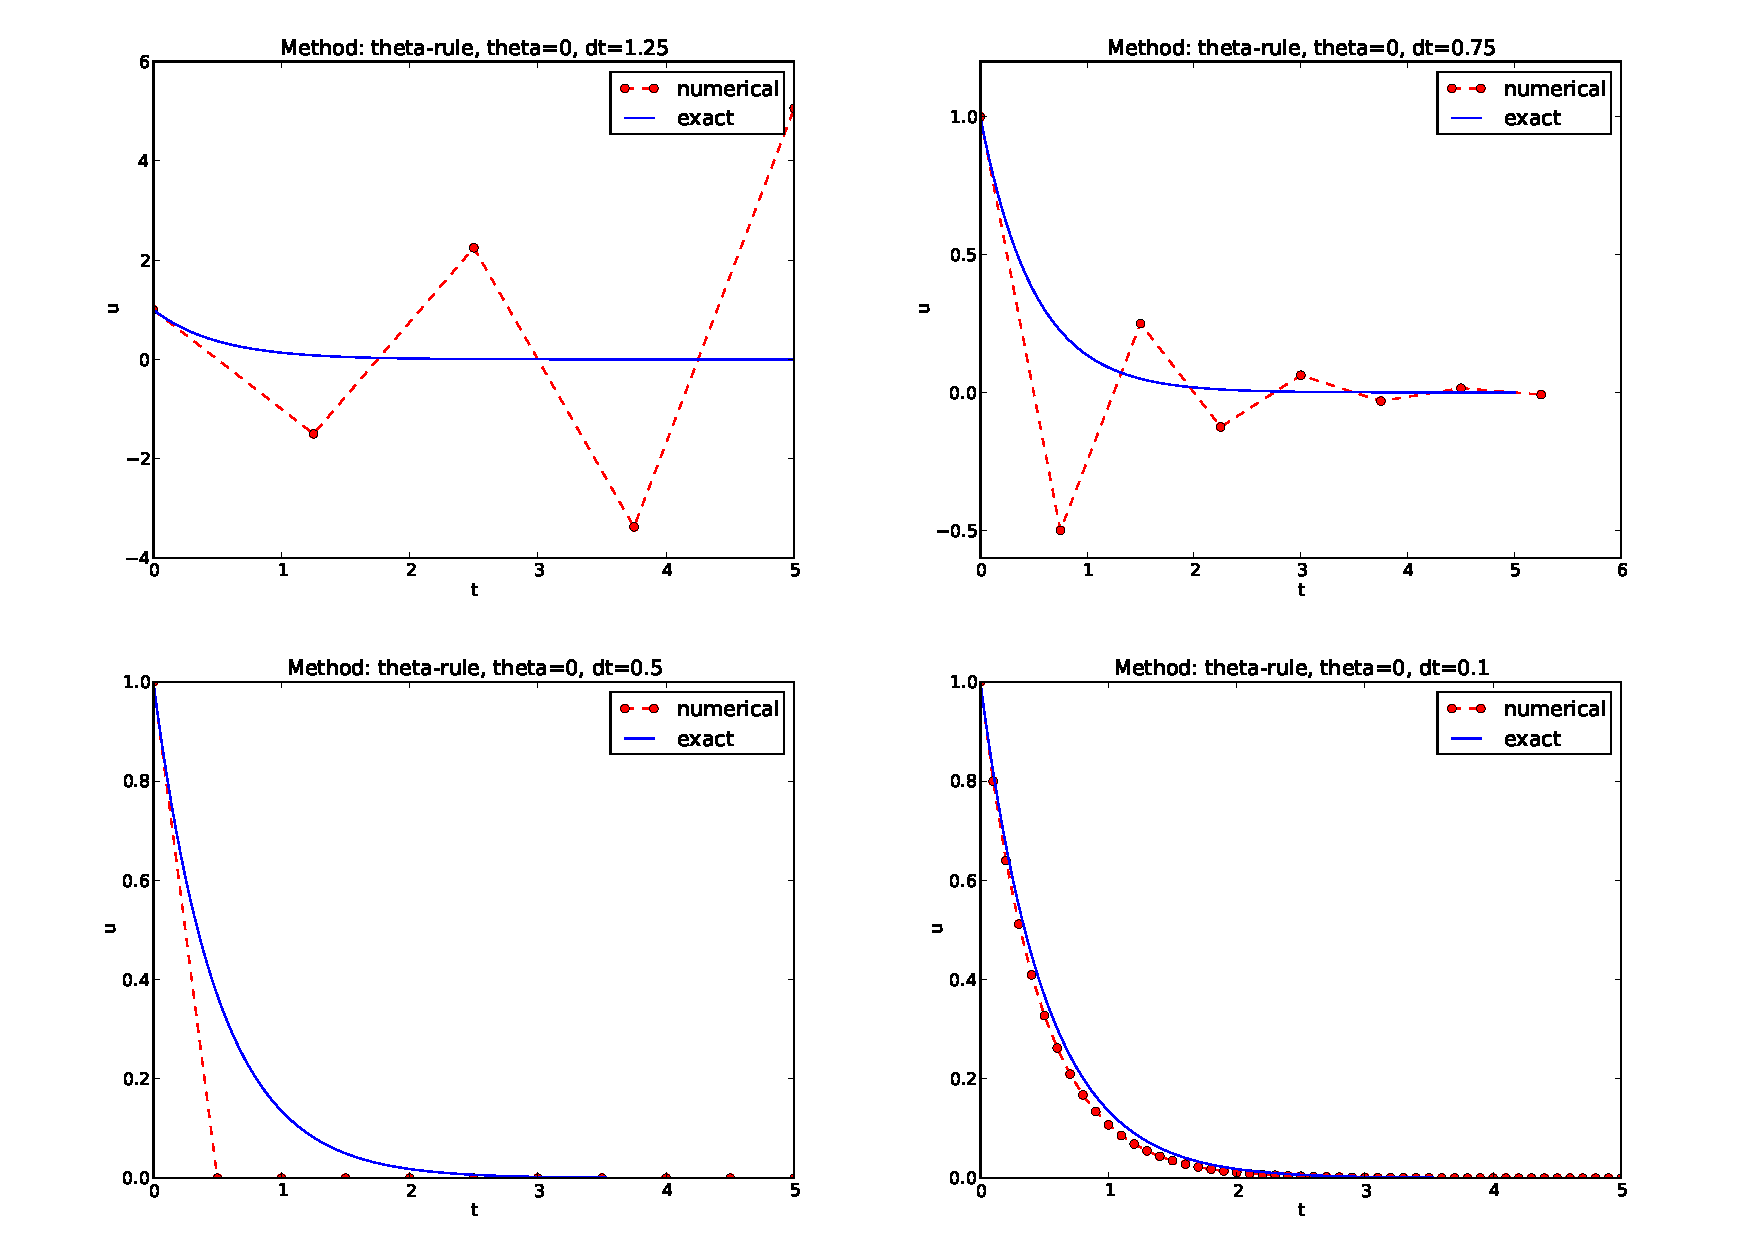
\includegraphics[width=1.1\linewidth]{fig-analysis/FE4c.pdf}}
  \caption{
  Forward Euler. \label{decay:analysis:FE4c}
  }
\end{figure}
%\clearpage % flush figures decay:analysis:FE4c


The characteristics of the displayed curves can be summarized as follows:

\begin{itemize}
  \item The Backward Euler scheme gives a monotone solution in all cases,
    lying above the exact curve.

  \item The Crank-Nicolson scheme gives the most accurate results, but for
    $\Delta t=1.25$ the solution oscillates.

  \item The Forward Euler scheme gives a growing, oscillating solution for
    $\Delta t=1.25$; a decaying, oscillating solution for $\Delta t=0.75$;
    a strange solution $u^n=0$ for $n\geq 1$ when $\Delta t=0.5$; and
    a solution seemingly as accurate as the one by the Backward Euler
    scheme for $\Delta t = 0.1$, but the curve lies below the exact
    solution.
\end{itemize}

\noindent
Since the exact solution of our model problem is a monotone function,
$u(t)=Ie^{-at}$, some of these qualitatively wrong results indeed seem alarming!


\begin{notice_mdfboxadmon}[Key questions]

\begin{itemize}
 \item Under what circumstances, i.e., values of
   the input data $I$, $a$, and $\Delta t$ will the Forward Euler and
   Crank-Nicolson schemes result in undesired oscillatory solutions?

 \item How does $\Delta t$ impact the error in the numerical solution?
\end{itemize}

\noindent
The first question will be investigated both by numerical experiments and
by precise mathematical theory. The theory will help establish
general criteria on $\Delta t$ for avoiding non-physical oscillatory
or growing solutions.

For our simple model problem we can answer the second
question very precisely, but
we will also look at simplified formulas for small $\Delta t$
and touch upon important concepts such as \emph{convergence rate} and
\emph{the order of a scheme}. Other fundamental concepts mentioned are
stability, consistency, and convergence.
\end{notice_mdfboxadmon}



\subsection{Detailed experiments}

To address the first question above,
we may set up an experiment where we loop over values of $I$, $a$,
and $\Delta t$ in our chosen model problem.
For each experiment, we flag the solution as
oscillatory if

\[ u^{n} > u^{n-1},\]
for some value of $n$. This seems like a reasonable choice,
since we expect $u^n$ to decay with $n$, but oscillations will make
$u$ increase over a time step. Doing some initial experimentation
with varying $I$, $a$, and $\Delta t$, quickly reveals that
oscillations are independent of $I$, but they do depend on $a$ and
$\Delta t$. We can therefore limit the investigation to
vary $a$ and $\Delta t$. Based on this observation,
we introduce a two-dimensional
function $B(a,\Delta t)$ which is 1 if oscillations occur
and 0 otherwise. We can visualize $B$ as a contour plot
(lines for which $B=\hbox{const}$). The contour $B=0.5$
corresponds to the borderline between oscillatory regions with $B=1$
and monotone regions with $B=0$ in the $a,\Delta t$ plane.

The $B$ function is defined at discrete $a$ and $\Delta t$ values.
Say we have given $P$ values for $a$, $a_0,\ldots,a_{P-1}$, and
$Q$ values for $\Delta t$, $\Delta t_0,\ldots,\Delta t_{Q-1}$.
These $a_i$ and $\Delta t_j$ values, $i=0,\ldots,P-1$,
$j=0,\ldots,Q-1$, form a rectangular mesh of $P\times Q$ points
in the plane spanned by $a$ and $\Delta t$.
At each point $(a_i, \Delta t_j)$, we associate
the corresponding value $B(a_i,\Delta t_j)$, denoted $B_{ij}$.
The $B_{ij}$ values are naturally stored in a two-dimensional
array. We can thereafter create a plot of the
contour line $B_{ij}=0.5$ dividing the oscillatory and monotone
regions. The file \href{{http://tinyurl.com/ofkw6kc/analysis/decay_osc_regions.py}}{\nolinkurl{decay_osc_regions.py}}  given below (\Verb!osc_regions! stands for ``oscillatory regions'') contains all nuts and
bolts to produce the $B=0.5$ line in Figures~\ref{decay:analysis:B:FE}
and~\ref{decay:analysis:B:CN}. The oscillatory region is above this line.

\begin{pro}{cbg_blue1}{bar_blue1}\begin{Verbatim}[numbers=none,fontsize=\fontsize{9pt}{9pt},baselinestretch=0.95,xleftmargin=2mm]
from decay_mod import solver
import numpy as np
import scitools.std as st

def non_physical_behavior(I, a, T, dt, theta):
    """
    Given lists/arrays a and dt, and numbers I, dt, and theta,
    make a two-dimensional contour line B=0.5, where B=1>0.5
    means oscillatory (unstable) solution, and B=0<0.5 means
    monotone solution of u'=-au.
    """
    a = np.asarray(a); dt = np.asarray(dt)  # must be arrays
    B = np.zeros((len(a), len(dt)))         # results
    for i in range(len(a)):
        for j in range(len(dt)):
            u, t = solver(I, a[i], T, dt[j], theta)
            # Does u have the right monotone decay properties?
            correct_qualitative_behavior = True
            for n in range(1, len(u)):
                if u[n] > u[n-1]:  # Not decaying?
                    correct_qualitative_behavior = False
                    break  # Jump out of loop
            B[i,j] = float(correct_qualitative_behavior)
    a_, dt_ = st.ndgrid(a, dt)  # make mesh of a and dt values
    st.contour(a_, dt_, B, 1)
    st.grid('on')
    st.title('theta=%g' % theta)
    st.xlabel('a'); st.ylabel('dt')
    st.savefig('osc_region_theta_%s.png' % theta)
    st.savefig('osc_region_theta_%s.pdf' % theta)

non_physical_behavior(
    I=1,
    a=np.linspace(0.01, 4, 22),
    dt=np.linspace(0.01, 4, 22),
    T=6,
    theta=0.5)
\end{Verbatim}
\end{pro}
\noindent


\begin{figure}[!ht]  % decay:analysis:B:FE
  \centerline{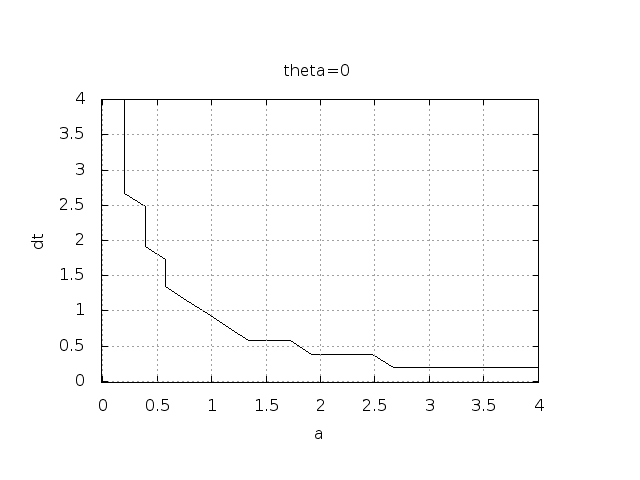
\includegraphics[width=0.9\linewidth]{fig-analysis/osc_region_FE.png}}
  \caption{
  Forward Euler scheme: oscillatory solutions occur for points above the curve. \label{decay:analysis:B:FE}
  }
\end{figure}
%\clearpage % flush figures decay:analysis:B:FE



\begin{figure}[!ht]  % decay:analysis:B:CN
  \centerline{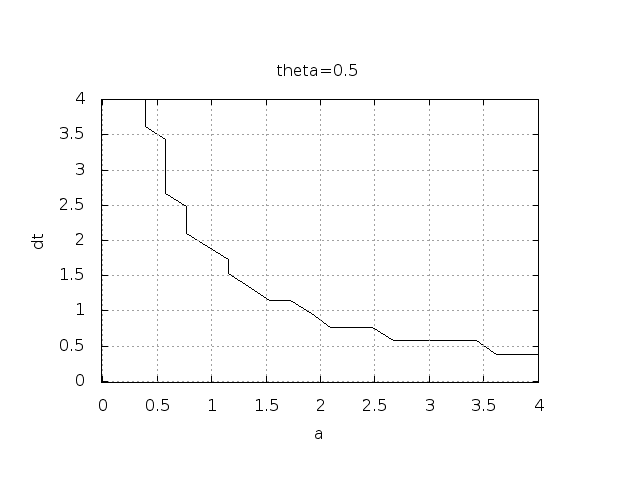
\includegraphics[width=0.9\linewidth]{fig-analysis/osc_region_CN.png}}
  \caption{
  Crank-Nicolson scheme: oscillatory solutions occur for points above the curve. \label{decay:analysis:B:CN}
  }
\end{figure}
%\clearpage % flush figures decay:analysis:B:CN


By looking at the curves in the figures one may guess that $a\Delta t$
must be less than a critical limit to avoid the undesired
oscillations.  This limit seems to be about 2 for Crank-Nicolson and 1
for Forward Euler.  We shall now establish a precise mathematical
analysis of the discrete model that can explain the observations in
our numerical experiments.


\section{Stability}

The goal now is to understand the results in the previous section.
To this end, we shall investigate the properties of the mathematical
formula for the solution of the equations arising from the finite
difference methods.

\subsection{Exact numerical solution}

Starting with $u^0=I$, the simple recursion (\ref{decay:analysis:scheme})
can be applied repeatedly $n$ times, with the result that
\begin{equation}
u^{n} = IA^n,\quad A = \frac{1 - (1-\theta) a\Delta t}{1 + \theta a\Delta t}\tp
\label{decay:analysis:unex}
\end{equation}


\begin{notice_mdfboxadmon}[Solving difference equations]
Difference equations where all terms are linear in
$u^{n+1}$, $u^n$, and maybe $u^{n-1}$, $u^{n-2}$, etc., are
called \emph{homogeneous, linear} difference equations, and their solutions
are generally of the form $u^n=A^n$, where $A$ is a constant to be
determined. Inserting this expression in the difference equation
and dividing by $A^{n+1}$ gives
a polynomial equation in $A$. In the present case we get

\[ A = \frac{1 - (1-\theta) a\Delta t}{1 + \theta a\Delta t}\tp \]
This is a solution technique of wider applicability than repeated use of
the recursion (\ref{decay:analysis:scheme}).
\end{notice_mdfboxadmon}



Regardless of the solution approach, we have obtained a formula for
$u^n$.  This formula can explain everything we see in the figures
above, but it also gives us a more general insight into accuracy and
stability properties of the three schemes.

\index{stability}

Since $u^n$ is a factor $A$
raised to an integer power $n$, we realize that $A < 0$
will imply $u^n < 0$ for odd $n$ and $u^n > 0$ for even $n$.
That is, the solution oscillates between the mesh points.
We have oscillations due to $A < 0$ when

\begin{equation}
(1-\theta)a\Delta t > 1 \tp
\label{decay:th:stability}
\end{equation}
Since $A>0$ is a requirement for having a numerical solution with the
same basic property (monotonicity) as the exact solution, we may say
that $A>0$ is a \emph{stability criterion}. Expressed in terms of $\Delta t$
the stability criterion reads

\begin{equation}
\Delta t < \frac{1}{(1-\theta)a}\tp
\end{equation}

The Backward
Euler scheme is always stable since $A < 0$ is impossible for $\theta=1$, while
non-oscillating solutions for Forward Euler and Crank-Nicolson
demand $\Delta t\leq 1/a$ and $\Delta t\leq 2/a$, respectively.
The relation between $\Delta t$ and $a$ look reasonable: a larger
$a$ means faster decay and hence a need for smaller time steps.

Looking at the upper left plot in Figure~\ref{decay:analysis:FE4c},
we see that $\Delta t=1.25$, and remembering that $a=2$ in these
experiments, $A$ can be calculated to be
$-1.5$, so the Forward Euler solution becomes $u^n=(-1.5)^n$ ($I=1$).
This solution oscillates \emph{and} grows. The upper right plot has
$a\Delta t = 2\cdot 0.75=1.5$, so $A=-0.5$,
and $u^n=(-0.5)^n$ decays but oscillates. The lower left plot
is a peculiar case where the Forward Euler scheme produces a solution
that is stuck on the $t$ axis. Now we can understand why this is so,
because $a\Delta t= 2\cdot 0.5=1$, which gives $A=0$,
and therefore $u^n=0$ for $n\geq 1$.  The decaying oscillations in the Crank-Nicolson scheme in the upper left plot in Figure~\ref{decay:analysis:CN4c}
for $\Delta t=1.25$ are easily explained by the fact that $A\approx -0.11 < 0$.


\subsection{Stability properties derived from the amplification factor}
\index{amplification factor}

The factor $A$ is called the \emph{amplification factor} since the solution
at a new time level is the solution at the previous time
level amplified by a factor $A$.
For a decay process, we must obviously have $|A|\leq 1$, which
is fulfilled for all $\Delta t$ if $\theta \geq 1/2$. Arbitrarily
large values of $u$ can be generated when $|A|>1$ and $n$ is large
enough. The numerical solution is in such cases totally irrelevant to
an ODE modeling decay processes! To avoid this situation, we must
demand $|A|\leq 1$ also for $\theta < 1/2$, which implies

\begin{equation}
\Delta t \leq \frac{2}{(1-2\theta)a},
\end{equation}
For example, $\Delta t$ must not exceed  $2/a$ when computing with
the Forward Euler scheme.

\index{A-stable methods}
\index{L-stable methods}


\begin{notice_mdfboxadmon}[Stability properties]
We may summarize the stability investigations as follows:

\begin{enumerate}
\item The Forward Euler method is a \emph{conditionally stable} scheme because
   it requires $\Delta t < 2/a$ for avoiding growing solutions
   and $\Delta t < 1/a$ for avoiding oscillatory solutions.

\item The Crank-Nicolson is \emph{unconditionally stable} with respect to
   growing solutions, while it is conditionally stable with
   the criterion $\Delta t < 2/a$ for avoiding oscillatory solutions.

\item The Backward Euler method is unconditionally stable with respect
   to growing and oscillatory solutions - any $\Delta t$ will work.
\end{enumerate}

\noindent
Much literature on ODEs speaks about L-stable and A-stable methods.
In our case A-stable methods ensures non-growing solutions, while
L-stable methods also avoids oscillatory solutions.
\end{notice_mdfboxadmon}



\section{Accuracy}

While stability concerns the qualitative properties of the numerical
solution, it remains to investigate the quantitative properties to
see exactly how large the numerical errors are.

\subsection{Visual comparison of amplification factors}

After establishing how $A$ impacts the qualitative features of the
solution, we shall now look more into how well the numerical amplification
factor approximates the exact one. The exact solution reads
$u(t)=Ie^{-at}$, which can be rewritten as
\begin{equation}
{\uex}(t_n) = Ie^{-a n\Delta t} = I(e^{-a\Delta t})^n \tp
\end{equation}
From this formula we see that the exact amplification factor is
\begin{equation}
\Aex = e^{-a\Delta t} \tp
\end{equation}

We see from all of our analysis
that the exact and numerical amplification factors depend
on $a$ and $\Delta t$ through the dimensionless
product $a\Delta t$: whenever there is a
$\Delta t$ in the analysis, there is always an associated $a$
parameter. Therefore, it
is convenient to introduce a symbol for this product, $p=a\Delta t$,
and view $A$ and $\Aex$ as functions of $p$. Figure~\ref{decay:analysis:fig:A} shows these functions. The two amplification
factors are clearly closest for the
Crank-Nicolson method, but that method has
the unfortunate oscillatory behavior when $p>2$.


\begin{figure}[!ht]  % decay:analysis:fig:A
  \centerline{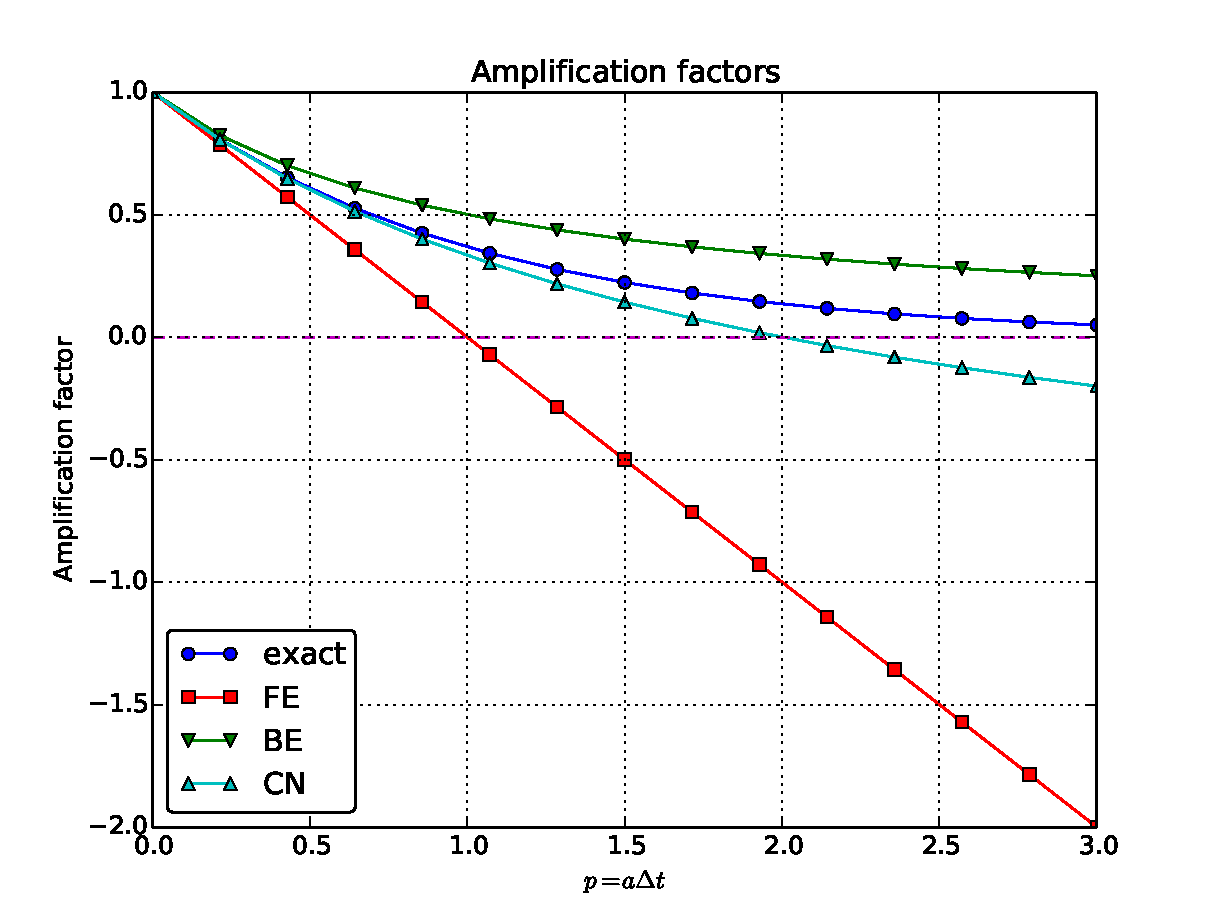
\includegraphics[width=0.9\linewidth]{fig-analysis/A_factors.pdf}}
  \caption{
  Comparison of amplification factors. \label{decay:analysis:fig:A}
  }
\end{figure}
%\clearpage % flush figures decay:analysis:fig:A




\begin{notice_mdfboxadmon}[Significance of the $p=a\Delta t$ parameter]
The key parameter for numerical performance of a scheme is in this model
problem $p=a\Delta t$. This is a \emph{dimensionless number} ($a$ has dimension
1/s and $\Delta t$ has dimension s) reflecting how the discretization
parameter plays together with a physical parameter in the problem.

One can bring the present model problem on dimensionless form
through a process called scaling. The scaled modeled has a modified
time $\bar t = at$ and modified response $\bar u =u/I$ such that
the model reads $d\bar u/d\bar t = -\bar u$, $\bar u(0)=1$.
Analyzing this model, where there are no physical parameters,
we find that $\Delta \bar t$ is the key parameter
for numerical performance. In the unscaled model,
this corresponds to $\Delta \bar t = a\Delta t$.

It is common that the numerical performance of methods for solving ordinary and
partial differential equations is governed by dimensionless parameters
that combine mesh sizes with physical parameters.
\end{notice_mdfboxadmon}



\subsection{Series expansion of amplification factors}

As an alternative to the visual understanding inherent in Figure~\ref{decay:analysis:fig:A}, there is a strong tradition in numerical
analysis to establish formulas for approximation errors when the
discretization parameter, here $\Delta t$, becomes small. In the
present case, we let $p$ be our small discretization parameter, and it
makes sense to simplify the expressions for $A$ and $\Aex$ by using
Taylor polynomials around $p=0$.  The Taylor polynomials are accurate
for small $p$ and greatly simplify the comparison of the analytical
expressions since we then can compare polynomials, term by term.

Calculating the Taylor series for $\Aex$ is easily done by hand, but
the three versions of $A$ for $\theta=0,1,{\half}$ lead to more
cumbersome calculations.
Nowadays, analytical computations can benefit greatly by
symbolic computer algebra software. The Python package \texttt{sympy}
represents a powerful computer algebra system, not yet as sophisticated as
the famous Maple and Mathematica systems, but it is free and
very easy to integrate with our numerical computations in Python.

\index{interactive Python}
\index{isympy@{\rm\texttt{isympy}}}
\index{sympy@{\rm\texttt{sympy}}}

When using \texttt{sympy}, it is convenient to enter an interactive Python
shell where the results of expressions and statements can be shown
immediately.
Here is a simple example. We strongly recommend to use
\texttt{isympy} (or \texttt{ipython}) for such interactive sessions.

Let us illustrate \texttt{sympy} with a standard Python shell syntax
(\texttt{>>>} prompt) to compute a Taylor polynomial approximation to $e^{-p}$:

\begin{cod}{cbg_blue1}\begin{Verbatim}[numbers=none,fontsize=\fontsize{9pt}{9pt},baselinestretch=0.95,xleftmargin=2mm]
>>> from sympy import *
>>> # Create p as a mathematical symbol with name 'p'
>>> p = Symbol('p')
>>> # Create a mathematical expression with p
>>> A_e = exp(-p)
>>>
>>> # Find the first 6 terms of the Taylor series of A_e
>>> A_e.series(p, 0, 6)
1 + (1/2)*p**2 - p - 1/6*p**3 - 1/120*p**5 + (1/24)*p**4 + O(p**6)
\end{Verbatim}
\end{cod}
\noindent
Lines with \texttt{>>>} represent input lines, whereas without
this prompt represent the result of the previous command (note that
\texttt{isympy} and \texttt{ipython} apply other prompts, but in this text
we always apply \texttt{>>>} for interactive Python computing).
Apart from the order of the powers, the computed formula is easily
recognized as the beginning of the Taylor series for $e^{-p}$.

Let us define the numerical amplification factor where $p$ and $\theta$
enter the formula as symbols:
\begin{cod}{cbg_blue1}\begin{Verbatim}[numbers=none,fontsize=\fontsize{9pt}{9pt},baselinestretch=0.95,xleftmargin=2mm]
>>> theta = Symbol('theta')
>>> A = (1-(1-theta)*p)/(1+theta*p)
\end{Verbatim}
\end{cod}
\noindent
To work with the factor for the Backward Euler scheme we
can substitute the value 1 for \texttt{theta}:

\begin{cod}{cbg_blue1}\begin{Verbatim}[numbers=none,fontsize=\fontsize{9pt}{9pt},baselinestretch=0.95,xleftmargin=2mm]
>>> A.subs(theta, 1)
1/(1 + p)
\end{Verbatim}
\end{cod}
\noindent
Similarly, we can substitute \texttt{theta} by 1/2 for Crank-Nicolson,
preferably using an exact rational representation of 1/2 in \texttt{sympy}:

\begin{cod}{cbg_blue1}\begin{Verbatim}[numbers=none,fontsize=\fontsize{9pt}{9pt},baselinestretch=0.95,xleftmargin=2mm]
>>> half = Rational(1,2)
>>> A.subs(theta, half)
1/(1 + (1/2)*p)*(1 - 1/2*p)
\end{Verbatim}
\end{cod}
\noindent

The Taylor series of the amplification factor for the Crank-Nicolson
scheme can be computed as

\begin{cod}{cbg_blue1}\begin{Verbatim}[numbers=none,fontsize=\fontsize{9pt}{9pt},baselinestretch=0.95,xleftmargin=2mm]
>>> A.subs(theta, half).series(p, 0, 4)
1 + (1/2)*p**2 - p - 1/4*p**3 + O(p**4)
\end{Verbatim}
\end{cod}
\noindent
We are now in a position to compare Taylor series:

\begin{cod}{cbg_blue1}\begin{Verbatim}[numbers=none,fontsize=\fontsize{9pt}{9pt},baselinestretch=0.95,xleftmargin=2mm]
>>> FE = A_e.series(p, 0, 4) - A.subs(theta, 0).series(p, 0, 4)
>>> BE = A_e.series(p, 0, 4) - A.subs(theta, 1).series(p, 0, 4)
>>> CN = A_e.series(p, 0, 4) - A.subs(theta, half).series(p, 0, 4 )
>>> FE
(1/2)*p**2 - 1/6*p**3 + O(p**4)
>>> BE
-1/2*p**2 + (5/6)*p**3 + O(p**4)
>>> CN
(1/12)*p**3 + O(p**4)
\end{Verbatim}
\end{cod}
\noindent
From these expressions we see that the error $A-\Aex\sim \Oof{p^2}$
for the Forward and Backward Euler schemes, while
$A-\Aex\sim \Oof{p^3}$ for the Crank-Nicolson scheme.
The notation $\Oof{p^m}$ here means a polynomial in $p$ where
$p^m$ is the term of lowest-degree, and consequently the term that
dominates the expression for $p < 0$. We call this the
\emph{leading order term}. As $p\rightarrow 0$, the leading order term
clearly dominates over the higher-order terms (think of $p=0.01$:
$p$ is a hundred times larger than $p^2$).

Now, $a$ is a given parameter in the problem, while $\Delta t$ is
what we can vary. Not surprisingly, the error expressions are usually
written in terms $\Delta t$. We then have

\begin{equation}
A-\Aex = \left\lbrace\begin{array}{ll}
\Oof{\Delta t^2}, & \hbox{Forward and Backward Euler},\\ 
\Oof{\Delta t^3}, & \hbox{Crank-Nicolson}
\end{array}\right.
\end{equation}

We say that the Crank-Nicolson scheme has an error in the amplification
factor of order $\Delta t^3$, while the two other schemes are
of order $\Delta t^2$ in the same quantity.

What is the significance of the order expression? If we halve $\Delta t$,
the error in amplification factor at a time level will be reduced
by a factor of 4 in the Forward and Backward Euler schemes, and by
a factor of 8 in the Crank-Nicolson scheme. That is, as we
reduce $\Delta t$ to obtain more accurate results, the Crank-Nicolson
scheme reduces the error more efficiently than the other schemes.


\subsection{The ratio of numerical and exact amplification factors}

\index{error!amplification factor}

An alternative comparison of the schemes is provided by looking at the
ratio $A/\Aex$, or the error $1-A/\Aex$ in this ratio:

\begin{cod}{cbg_blue1}\begin{Verbatim}[numbers=none,fontsize=\fontsize{9pt}{9pt},baselinestretch=0.95,xleftmargin=2mm]
>>> FE = 1 - (A.subs(theta, 0)/A_e).series(p, 0, 4)
>>> BE = 1 - (A.subs(theta, 1)/A_e).series(p, 0, 4)
>>> CN = 1 - (A.subs(theta, half)/A_e).series(p, 0, 4)
>>> FE
(1/2)*p**2 + (1/3)*p**3 + O(p**4)
>>> BE
-1/2*p**2 + (1/3)*p**3 + O(p**4)
>>> CN
(1/12)*p**3 + O(p**4)
\end{Verbatim}
\end{cod}
\noindent
The leading-order terms have the same powers as
in the analysis of $A-\Aex$.

\subsection{The global error at a point}
\label{decay:analysis:gobal:error}

\index{error!global}

The error in the amplification factor reflects the error when
progressing from time level $t_n$ to $t_{n-1}$ only. That is,
we disregard the error already present in the solution at $t_{n-1}$.
The real error at a point, however, depends on the error development
over all previous time steps. This error,
$e^n = u^n-\uex(t_n)$, is known as the \emph{global error}. We
may look at $u^n$ for some $n$ and Taylor expand the
mathematical expressions as functions of $p=a\Delta t$ to get a simple
expression for the global error (for small $p$):

\begin{cod}{cbg_blue1}\begin{Verbatim}[numbers=none,fontsize=\fontsize{9pt}{9pt},baselinestretch=0.95,xleftmargin=2mm]
>>> n = Symbol('n')
>>> u_e = exp(-p*n)
>>> u_n = A**n
>>> FE = u_e.series(p, 0, 4) - u_n.subs(theta, 0).series(p, 0, 4)
>>> BE = u_e.series(p, 0, 4) - u_n.subs(theta, 1).series(p, 0, 4)
>>> CN = u_e.series(p, 0, 4) - u_n.subs(theta, half).series(p, 0, 4)
>>> FE
(1/2)*n*p**2 - 1/2*n**2*p**3 + (1/3)*n*p**3 + O(p**4)
>>> BE
(1/2)*n**2*p**3 - 1/2*n*p**2 + (1/3)*n*p**3 + O(p**4)
>>> CN
(1/12)*n*p**3 + O(p**4)
\end{Verbatim}
\end{cod}
\noindent
Note that \texttt{sympy} does not sort the polynomial terms in the output,
so $p^3$ appears before $p^2$ in the output of \texttt{BE}.

For a fixed time $t$, the parameter $n$ in these expressions increases
as $p\rightarrow 0$ since $t=n\Delta t =\mbox{const}$ and hence
$n$ must increase like $\Delta t^{-1}$. With $n$ substituted by
$t/\Delta t$ in
the leading-order error terms, these become

\begin{align}
e^n &= \half n p^2 = {\half}ta^2\Delta t, &\hbox{Forward Euler}
\label{decay:analysis:gobal:error:FE}\\ 
e^n &= -\half n p^2 = -{\half}ta^2\Delta t, &\hbox{Backward Euler}
\label{decay:analysis:gobal:error:BE}\\ 
e^n &= \frac{1}{12}np^3 = \frac{1}{12}ta^3\Delta t^2, &\hbox{Crank-Nicolson}
\label{decay:analysis:gobal:error:CN}
\end{align}
The global error is therefore of
second order (in $\Delta t$) for the Crank-Nicolson scheme and of
first order for the other two schemes.


\begin{notice_mdfboxadmon}[Convergence]
When the global error $e^n\rightarrow 0$ as $\Delta t\rightarrow 0$,
we say that the scheme is \emph{convergent}. It means that the numerical
solution approaches the exact solution as the mesh is refined, and
this is a much desired property of a numerical method.
\end{notice_mdfboxadmon}



\subsection{Integrated error}
\label{decay:analysis:gobal:error_int}

It is common to study the norm of the numerical error, as
explained in detail in Section~\ref{decay:computing:error:norm}.
The $L^2$ norm of the error can be computed by treating $e^n$ as a function
of $t$ in \texttt{sympy} and performing symbolic integration. For
the Forward Euler scheme we have

\begin{cod}{cbg_blue1}\begin{Verbatim}[numbers=none,fontsize=\fontsize{9pt}{9pt},baselinestretch=0.95,xleftmargin=2mm]
p, n, a, dt, t, T, theta = symbols('p n a dt t T 'theta')
A = (1-(1-theta)*p)/(1+theta*p)
u_e = exp(-p*n)
u_n = A**n
error = u_e.series(p, 0, 4) - u_n.subs(theta, 0).series(p, 0, 4)
# Introduce t and dt instead of n and p
error = error.subs('n', 't/dt').subs(p, 'a*dt')
error = error.as_leading_term(dt) # study only the first term
print error
error_L2 = sqrt(integrate(error**2, (t, 0, T)))
print error_L2
\end{Verbatim}
\end{cod}
\noindent
The output reads

\begin{cod}{cbg_blue1}\begin{Verbatim}[numbers=none,fontsize=\fontsize{9pt}{9pt},baselinestretch=0.95,xleftmargin=2mm]
sqrt(30)*sqrt(T**3*a**4*dt**2*(6*T**2*a**2 - 15*T*a + 10))/60
\end{Verbatim}
\end{cod}
\noindent
which means that the $L^2$ error behaves like $a^2\Delta t$.

Strictly speaking, the numerical error is only defined at the
mesh points so it makes most sense to compute the
$\ell^2$ error

\[ ||e^n||_{\ell^2} = \sqrt{\Delta t\sum_{n=0}^{N_t} ({\uex}(t_n) - u^n)^2}
\tp \]
We have obtained an exact analytical expression for the error at
$t=t_n$, but here we use the leading-order error term only since we
are mostly interested in how the error behaves as a polynomial in
$\Delta t$ or $p$, and then the leading order term will dominate.  For
the Forward Euler scheme, $\uex(t_n) - u^n \approx {\half}np^2$, and
we have

\[
||e^n||_{\ell^2}^2 = \Delta t\sum_{n=0}^{N_t} \frac{1}{4}n^2p^4
=\Delta t\frac{1}{4}p^4 \sum_{n=0}^{N_t} n^2\tp
\]
Now, $\sum_{n=0}^{N_t} n^2\approx \frac{1}{3}N_t^3$. Using this approximation,
setting $N_t =T/\Delta t$, and taking the square root gives the expression

\begin{equation}
||e^n||_{\ell^2} = \half\sqrt{\frac{T^3}{3}} a^2\Delta t\tp
\label{decay:analysis:gobal:error_int:FE}
\end{equation}
Calculations for the Backward Euler scheme are very similar and provide
the same result, while the Crank-Nicolson scheme leads to

\begin{equation}
||e^n||_{\ell^2} = \frac{1}{12}\sqrt{\frac{T^3}{3}}a^3\Delta t^2\tp
\label{decay:analysis:gobal:error_int:CN}
\end{equation}


\begin{summary_mdfboxadmon}[Summary of errors]
Both the global point-wise errors (\ref{decay:analysis:gobal:error:FE})-(\ref{decay:analysis:gobal:error:CN})
and their time-integrated versions (\ref{decay:analysis:gobal:error_int:FE}) and (\ref{decay:analysis:gobal:error_int:CN}) show that

\begin{itemize}
 \item the Crank-Nicolson scheme is of second order in $\Delta t$, and

 \item the Forward Euler and Backward Euler schemes are of first order in $\Delta t$.
\end{itemize}

\noindent
\end{summary_mdfboxadmon}



\subsection{Truncation error}
\label{decay:analysis:trunc}

The truncation error is a very frequently used error measure for
finite difference methods. It is defined as \emph{the error
in the difference equation that arises when inserting the exact
solution}. Contrary to many other error measures, e.g., the
true error $e^n=\uex(t_n)-u^n$, the truncation error is a quantity that
is easily computable.

Before reading on, it is wise to review Section~\ref{decay:fd:taylor}
on how Taylor polynomials were used to derive finite differences and
quantify the error in the formulas. Very similar reasoning, and almost
identical mathematical details, will be carried out below, but in a slightly
different context. Now, the
focus is on the error when solving a differential
equation, while in Section~\ref{decay:fd:taylor} we derived
errors for a finite difference formula. These errors are tightly
connected in the present model problem.

Let us illustrate the calculation of the truncation error
for the Forward Euler scheme.
We start with the difference equation on operator form,

\[ \lbrack D_t^+ u = -au\rbrack^n,\]
which is the short form for

\[ \frac{u^{n+1}-u^n}{\Delta t} = -au^n\tp\]
The idea is to see how well the exact solution $\uex(t)$ fulfills
this equation. Since $\uex(t)$ in general will not obey the
discrete equation, we get an error in the discrete equation. This
error is called
a \emph{residual}, denoted here by $R^n$:

\begin{equation}
R^n = \frac{\uex(t_{n+1})-\uex(t_n)}{\Delta t} + a\uex(t_n)
\tp
\label{decay:analysis:trunc:Req}
\end{equation}
The residual is defined at each mesh point and is therefore a mesh
function with a superscript $n$.

The interesting feature of $R^n$ is to see how it
depends on the discretization parameter $\Delta t$.
The tool for reaching
this goal is to Taylor expand $\uex$ around the point where the
difference equation is supposed to hold, here $t=t_n$.
We have that

\[ \uex(t_{n+1}) = \uex(t_n) + \uex'(t_n)\Delta t + \half\uex''(t_n)
\Delta t^2 + \cdots, \]
which may be used to reformulate the fraction in
(\ref{decay:analysis:trunc:Req}) so that

\[ R^n = \uex'(t_n) + \half\uex''(t_n)\Delta t + \ldots + a\uex(t_n)\tp\]
Now, $\uex$ fulfills the ODE $\uex'=-a\uex$, which means that the first and last
term cancel and we have

\[ R^n = \half\uex''(t_n)\Delta t + \Oof{\Delta t^2}\tp \]
This $R^n$ is the \emph{truncation error}, which for the Forward Euler is seen
to be of first order in $\Delta t$ as $\Delta \rightarrow 0$.

The above procedure can be repeated for the Backward Euler and the
Crank-Nicolson schemes. We start with the scheme in operator notation,
write it out in detail, Taylor expand $\uex$ around the point $\tilde t$
at which the difference equation is defined, collect terms that
correspond to the ODE (here $\uex' + a\uex$), and identify the remaining
terms as the residual $R$, which is the truncation error.
The Backward Euler scheme leads to

\[ R^n \approx -\half\uex''(t_n)\Delta t, \]
while the Crank-Nicolson scheme gives

\[ R^{n+\half} \approx \frac{1}{24}\uex'''(t_{n+\half})\Delta t^2,\]
when $\Delta t\rightarrow 0$.

The \emph{order} $r$ of a finite difference scheme is often defined through
the leading term $\Delta t^r$ in the truncation error. The above
expressions point out that the Forward and Backward Euler schemes are
of first order, while Crank-Nicolson is of second order.  We have
looked at other error measures in other sections, like the error in
amplification factor and the error $e^n=\uex(t_n)-u^n$, and expressed
these error measures in terms of $\Delta t$ to see the order of the
method. Normally, calculating the truncation error is more
straightforward than deriving the expressions for other error measures
and therefore the easiest way to establish the order of a scheme.

\subsection{Consistency, stability, and convergence}

\index{consistency} \index{stability} \index{convergence}

Three fundamental concepts when solving differential equations by
numerical methods are consistency, stability, and convergence.  We
shall briefly touch upon these concepts below in the context of the present
model problem.

Consistency means that the error in the difference equation, measured
through the truncation error, goes to zero as $\Delta t\rightarrow
0$. Since the truncation error tells how well the exact solution
fulfills the difference equation, and the exact solution fulfills the
differential equation, consistency ensures that the difference
equation approaches the differential equation in the limit. The
expressions for the truncation errors in the previous section are all
proportional to $\Delta t$ or $\Delta t^2$, hence they vanish as
$\Delta t\rightarrow 0$, and all the schemes are consistent.  Lack of
consistency implies that we actually solve some other differential
equation in the limit $\Delta t\rightarrow 0$ than we aim at.

Stability means that the numerical solution exhibits the same
qualitative properties as the exact solution. This is obviously a
feature we want the numerical solution to have. In the present
exponential decay model, the exact solution is monotone and
decaying. An increasing numerical solution is not in accordance with
the decaying nature of the exact solution and hence unstable. We can
also say that an oscillating numerical solution lacks the property of
monotonicity of the exact solution and is also unstable. We have seen
that the Backward Euler scheme always leads to monotone and decaying
solutions, regardless of $\Delta t$, and is hence stable. The Forward
Euler scheme can lead to increasing solutions and oscillating
solutions if $\Delta t$ is too large and is therefore unstable unless
$\Delta t$ is sufficiently small.  The Crank-Nicolson can never lead
to increasing solutions and has no problem to fulfill that stability
property, but it can produce oscillating solutions and is unstable in
that sense, unless $\Delta t$ is sufficiently small.

Convergence implies that the global (true) error mesh function $e^n =
\uex(t_n)-u^n\rightarrow 0$ as $\Delta t\rightarrow 0$. This is really
what we want: the numerical solution gets as close to the exact
solution as we request by having a sufficiently fine mesh.

Convergence is hard to establish theoretically, except in quite simple
problems like the present one. Stability and consistency are much
easier to calculate. A major breakthrough in the understanding of
numerical methods for differential equations came in 1956 when Lax and
Richtmeyer established equivalence between convergence on one hand and
consistency and stability on the other (the \href{{http://en.wikipedia.org/wiki/Lax_equivalence_theorem}}{Lax equivalence theorem}).  In practice
it meant that one can first establish that a method is stable and
consistent, and then it is automatically convergent (which is much
harder to establish).  The result holds for linear problems only, and
in the world of nonlinear differential equations the relations between
consistency, stability, and convergence are much more complicated.

We have seen in the previous analysis that the Forward Euler,
Backward Euler, and Crank-Nicolson schemes are convergent ($e^n\rightarrow 0$),
that they are consistent ($R^n\rightarrow 0$), and that they are
stable under certain conditions on the size of $\Delta t$.
We have also derived explicit mathematical expressions for $e^n$,
the truncation error, and the stability criteria.

% Look in Asher and Petzold, p 40

\section{Exercises}



% --- begin exercise ---
\begin{doconceexercise}
\refstepcounter{doconceexercisecounter}

\subsection*{Problem \thedoconceexercisecounter: Visualize the accuracy of finite differences}
\addcontentsline{loe}{doconceexercise}{Problem \thedoconceexercisecounter: Visualize the accuracy of finite differences}

\label{decay:analysis:exer:fd:exp:plot}

The purpose of this exercise is to visualize the accuracy of finite difference
approximations of the derivative of a given function.
For any finite difference approximation, take the Forward Euler difference
as an example, and any specific function, take  $u=e^{-at}$,
we may introduce an error fraction

\begin{align*}
E = \frac{[D_t^+ u]^n}{u'(t_n)} &= \frac{\exp{(-a(t_n+\Delta t))} - \exp{(-at_n)}}{-a\exp{(-at_n)\Delta t}}\\ 
&= \frac{1}{a\Delta t}\left(1 -\exp{(-a\Delta t)}\right),
\end{align*}
and view $E$ as a function of $\Delta t$. We expect that
$\lim_{\Delta t\rightarrow 0}E=1$, while $E$ may deviate significantly from
unity for large $\Delta t$. How the error depends on $\Delta t$ is best
visualized in a graph where we use a logarithmic scale for $\Delta t$,
so we can cover many orders of magnitude of that quantity. Here is
a code segment creating an array of 100 intervals, on the logarithmic
scale, ranging from $10^{-6}$ to $10^{-0.5}$ and then plotting $E$ versus
$p=a\Delta t$ with logarithmic scale on the $p$ axis:

\begin{cod}{cbg_blue1}\begin{Verbatim}[numbers=none,fontsize=\fontsize{9pt}{9pt},baselinestretch=0.95,xleftmargin=2mm]
from numpy import logspace, exp
from matplotlib.pyplot import semilogx
p = logspace(-6, -0.5, 101)
y = (1-exp(-p))/p
semilogx(p, y)
\end{Verbatim}
\end{cod}
\noindent
Illustrate such errors for the finite difference operators $[D_t^+u]^n$
(forward), $[D_t^-u]^n$ (backward), and $[D_t u]^n$ (centered) in
the same plot.

Perform a Taylor series expansions of the error fractions and find
the leading order $r$ in the expressions of type
$1 + Cp^r + \Oof{p^{r+1}}$, where $C$ is some constant.

% --- begin hint in exercise ---

\paragraph{Hint.}
To save manual calculations and learn more about symbolic computing,
make functions for the three difference operators and use \texttt{sympy}
to perform the symbolic differences, differentiation, and Taylor series
expansion. To plot a symbolic expression \texttt{E} against \texttt{p}, convert the
expression to a Python function first: \texttt{E = sympy.lamdify([p], E)}.

% --- end hint in exercise ---


% removed !bsol ... !esol environment (because of the command-line option --without_solutions)
\noindent Filename: \Verb!decay_plot_fd_error!.

\end{doconceexercise}
% --- end exercise ---




% --- begin exercise ---
\begin{doconceexercise}
\refstepcounter{doconceexercisecounter}

\subsection*{Problem \thedoconceexercisecounter: Explore the $\theta$-rule for exponential growth}
\addcontentsline{loe}{doconceexercise}{Problem \thedoconceexercisecounter: Explore the $\theta$-rule for exponential growth}

\label{decay:analysis:exer:growth}

This exercise asks you to solve the ODE $u'=-au$ with $a < 0$ such that
the ODE models exponential growth instead of exponential decay.  A
central theme is to investigate numerical artifacts and non-physical
solution behavior.


\subex{a)}
Set $a=-1$ and run experiments with $\theta=0, 0.5, 1$ for
various values of $\Delta t$ to uncover numerical artifacts.
Recall that the exact solution is a
monotone, growing function when $a < 0$. Oscillations or significantly
wrong growth are signs of wrong qualitative behavior.

From the experiments, select four values of $\Delta t$ that
demonstrate the kind of numerical solutions that are characteristic
for this model.


% removed !bsol ... !esol environment (because of the command-line option --without_solutions)

\subex{b)}
Write up the amplification factor and plot it for $\theta=0,0.5,1$
together with the exact one for $a\Delta t < 0$. Use the plot to
explain the observations made in the experiments.

% --- begin hint in exercise ---

\paragraph{Hint.}
Modify the \href{{http://tinyurl.com/ofkw6kc/analysis/decay_ampf_plot.py}}{\nolinkurl{decay_ampf_plot.py}} code
(in the \texttt{src/analysis} directory).

% --- end hint in exercise ---


% removed !bsol ... !esol environment (because of the command-line option --without_solutions)

\noindent Filename: \Verb!exponential_growth!.

\end{doconceexercise}
% --- end exercise ---


% !split
\chapter{Generalizations}

It is time to consider generalizations of the simple decay model
$u^{\prime}=-au$ and also to look at additional numerical solution
methods.  We consider first variable coefficients, $u^{\prime}=a(t)u +
b(t)$, and later a completely general scalar ODE $u^{\prime}=f(u,t)$
and its generalization to a system of such general ODEs.  Among
numerical methods, we treat implicit multi-step methods, and several
families of explicit methods: Leapfrog schemes, Runge-Kutta methods,
and Adams-Bashforth formulas.

\section{Model extensions}

This section looks at the generalizations to $u^{\prime}=-a(t)u$
and $u^{\prime}=-a(t)u + b(t)$. We sketch the corresponding
implementations of the $\theta$-rule for such variable-coefficient ODEs.
Verification can no longer make use of an exact solution of the
numerical problem so we make use of manufactured solutions,
for deriving an exact solution of the ODE problem, and then we can
compute empirical convergence rates for the method and see if these
coincide with the expected rates from theory.
Finally, we see how our numerical methods can be applied to systems
of ODEs.

The example programs associated with this chapter are found in
the directory \href{{http://tinyurl.com/ofkw6kc/genz}}{\nolinkurl{src/genz}}.


\subsection{Generalization: including a variable coefficient}

In the ODE for decay, $u^{\prime}=-au$, we now consider the case where $a$
depends on time:

\begin{equation}
u^{\prime}(t) = -a(t)u(t),\quad t\in (0,T],\quad u(0)=I \tp
\label{decay:problem:a}
\end{equation}

A Forward Euler scheme consists of evaluating (\ref{decay:problem:a})
at $t=t_n$ and approximating the derivative with a forward
difference $[D^+_t u]^n$:

\begin{equation}
\frac{u^{n+1} - u^n}{\Delta t} = -a(t_n)u^n
\tp
\end{equation}
The Backward Euler scheme becomes
\begin{equation}
\frac{u^{n} - u^{n-1}}{\Delta t} = -a(t_n)u^n
\tp
\end{equation}
The Crank-Nicolson method builds on sampling the ODE at
$t_{n+\half}$. We can evaluate $a$ at $t_{n+\half}$
and use an average for $u$ at
times $t_n$ and $t_{n+1}$:
\begin{equation}
\frac{u^{n+1} - u^{n}}{\Delta t} = -a(t_{n+\half})\half(u^n + u^{n+1})
\tp
\end{equation}
Alternatively, we can use an average for the product $au$:

\begin{equation}
\frac{u^{n+1} - u^{n}}{\Delta t} = -\half(a(t_n)u^n + a(t_{n+1})u^{n+1})
\tp
\end{equation}
The $\theta$-rule unifies the three mentioned schemes. One version is to
have $a$ evaluated at the weighted time point $(1-\theta)t_n + \theta t_{n+1}$,

\begin{equation}
\frac{u^{n+1} - u^{n}}{\Delta t} = -a((1-\theta)t_n + \theta t_{n+1})((1-\theta) u^n + \theta u^{n+1})
\tp
\end{equation}
Another possibility is to apply a weighted average for the product $au$,
\begin{equation}
\frac{u^{n+1} - u^{n}}{\Delta t} = -(1-\theta) a(t_n)u^n - \theta
a(t_{n+1})u^{n+1}
\tp
\end{equation}

With the finite difference operator notation the Forward Euler and Backward
Euler schemes can be summarized as

\begin{align}
\lbrack D^+_t u &= -au\rbrack^n,\\ 
\lbrack D^-_t u &= -au\rbrack^n
\tp
\end{align}
The Crank-Nicolson and $\theta$ schemes depend on whether we evaluate
$a$ at the sample point for the ODE or if we use an average. The
various versions are written as

\begin{align}
\lbrack D_t u &= -a\overline{u}^t\rbrack^{n+\half},\\ 
\lbrack D_t u &= -\overline{au}^t\rbrack^{n+\half},\\ 
\lbrack D_t u &= -a\overline{u}^{t,\theta}\rbrack^{n+\theta},\\ 
\lbrack D_t u &= -\overline{au}^{t,\theta}\rbrack^{n+\theta}
\tp
\end{align}


\subsection{Generalization: including a source term}
\label{decay:source}

A further extension of the model ODE is to include a source term $b(t)$:

\begin{equation}
u^{\prime}(t) = -a(t)u(t) + b(t),\quad t\in (0,T],\quad u(0)=I
\tp
\label{decay:problem:ab}
\end{equation}

The time point where we sample the ODE determines where $b(t)$ is
evaluated. For the Crank-Nicolson scheme and the $\theta$-rule we
have a choice of whether to evaluate $a(t)$ and $b(t)$ at the
correct point or use an average. The chosen strategy becomes
particularly clear if we write up the schemes in the operator notation:

\begin{align}
\lbrack D^+_t u &= -au + b\rbrack^n,\\ 
\lbrack D^-_t u &= -au + b\rbrack^n,\\ 
\lbrack D_t u   &= -a\overline{u}^t + b\rbrack^{n+\half},\\ 
\lbrack D_t u   &= \overline{-au+b}^t\rbrack^{n+\half},\\ 
\lbrack D_t u   &= -a\overline{u}^{t,\theta} + b\rbrack^{n+\theta},\\ 
\lbrack D_t u   &= \overline{-au+b}^{t,\theta}\rbrack^{n+\theta}
\label{decay:problem:ab:theta:avg:all:op}
\tp
\end{align}

\subsection{Implementation of the generalized model problem}
\label{decay:general}

\paragraph{Deriving the $\theta$-rule formula.}
Writing out the $\theta$-rule in (\ref{decay:problem:ab:theta:avg:all:op}),
using (\ref{decay:fd1:Du:theta})
and (\ref{decay:fd1:wmean:a}), we get
\begin{equation}
\frac{u^{n+1}-u^n}{\Delta t} = \theta(-a^{n+1}u^{n+1} + b^{n+1}))
+ (1-\theta)(-a^nu^{n} + b^n)),
\label{decay:problem:ab:theta:avg:all}
\end{equation}
where $a^n$ means evaluating $a$ at $t=t_n$ and similar for
$a^{n+1}$, $b^n$, and $b^{n+1}$.
We solve for $u^{n+1}$:
\begin{equation}
u^{n+1} = ((1 - \Delta t(1-\theta)a^n)u^n
+ \Delta t(\theta b^{n+1} + (1-\theta)b^n))(1 + \Delta t\theta a^{n+1})^{-1}
\tp
\end{equation}

\paragraph{Python code.}
Here is a suitable implementation of (\ref{decay:problem:ab:theta:avg:all})
where $a(t)$ and $b(t)$ are given as
Python functions:

\begin{cod}{cbg_blue1}\begin{Verbatim}[numbers=none,fontsize=\fontsize{9pt}{9pt},baselinestretch=0.95,xleftmargin=2mm]
def solver(I, a, b, T, dt, theta):
    """
    Solve u'=-a(t)*u + b(t), u(0)=I,
    for t in (0,T] with steps of dt.
    a and b are Python functions of t.
    """
    dt = float(dt)            # avoid integer division
    Nt = int(round(T/dt))     # no of time intervals
    T = Nt*dt                 # adjust T to fit time step dt
    u = zeros(Nt+1)           # array of u[n] values
    t = linspace(0, T, Nt+1)  # time mesh

    u[0] = I                  # assign initial condition
    for n in range(0, Nt):    # n=0,1,...,Nt-1
        u[n+1] = ((1 - dt*(1-theta)*a(t[n]))*u[n] + \ 
                  dt*(theta*b(t[n+1]) + (1-theta)*b(t[n])))/\ 
                  (1 + dt*theta*a(t[n+1]))
    return u, t
\end{Verbatim}
\end{cod}
\noindent
This function is found in the file \href{{http://tinyurl.com/ofkw6kc/genz/decay_vc.py}}{\nolinkurl{decay_vc.py}} (\texttt{vc} stands for ``variable coefficients'').

\paragraph{Coding of variable coefficients.}
The \texttt{solver} function shown above demands the arguments \texttt{a} and \texttt{b} to
be Python functions of time \texttt{t}, say

\begin{cod}{cbg_blue1}\begin{Verbatim}[numbers=none,fontsize=\fontsize{9pt}{9pt},baselinestretch=0.95,xleftmargin=2mm]
def a(t):
    return a_0 if t < tp else k*a_0

def b(t):
    return 1
\end{Verbatim}
\end{cod}
\noindent
Here, \texttt{a(t)} has three parameters \texttt{a0}, \texttt{tp}, and \texttt{k},
which must be global variables.

A better implementation, which avoids global variables,
is to represent \texttt{a} by a class where the
parameters are attributes and where a \emph{special method} \Verb!__call__!
evaluates $a(t)$:

\begin{cod}{cbg_blue1}\begin{Verbatim}[numbers=none,fontsize=\fontsize{9pt}{9pt},baselinestretch=0.95,xleftmargin=2mm]
class A:
    def __init__(self, a0=1, k=2):
        self.a0, self.k = a0, k

    def __call__(self, t):
        return self.a0 if t < self.tp else self.k*self.a0

a = A(a0=2, k=1)  # a behaves as a function a(t)
\end{Verbatim}
\end{cod}
\noindent

\index{lambda functions}

For quick tests it is cumbersome to write a complete function or a class.
The \emph{lambda function} construction in Python is then convenient. For example,
\begin{cod}{cbg_blue1}\begin{Verbatim}[numbers=none,fontsize=\fontsize{9pt}{9pt},baselinestretch=0.95,xleftmargin=2mm]
a = lambda t: a_0 if t < tp else k*a_0
\end{Verbatim}
\end{cod}
\noindent
is equivalent to the \texttt{def a(t)} definition above. In general,
\begin{cod}{cbg_blue1}\begin{Verbatim}[numbers=none,fontsize=\fontsize{9pt}{9pt},baselinestretch=0.95,xleftmargin=2mm]
f = lambda arg1, arg2, ...: expression
\end{Verbatim}
\end{cod}
\noindent
is equivalent to
\begin{cod}{cbg_blue1}\begin{Verbatim}[numbers=none,fontsize=\fontsize{9pt}{9pt},baselinestretch=0.95,xleftmargin=2mm]
def f(arg1, arg2, ...):
    return expression
\end{Verbatim}
\end{cod}
\noindent
One can use lambda functions directly in calls. Say we want to
solve $u^{\prime}=-u+1$, $u(0)=2$:
\begin{cod}{cbg_blue1}\begin{Verbatim}[numbers=none,fontsize=\fontsize{9pt}{9pt},baselinestretch=0.95,xleftmargin=2mm]
u, t = solver(2, lambda t: 1, lambda t: 1, T, dt, theta)
\end{Verbatim}
\end{cod}
\noindent

Whether to use a plain function, a class, or a lambda function depends
on the programmer's taste. Lazy programmers prefer the lambda construct, while
very safe programmers go for the class solution.

\subsection{Verifying a constant solution}
\label{decay:verify:trivial}

An extremely useful partial verification method is to construct a test
problem with a very simple solution, usually $u=\hbox{const}$.
Especially the initial debugging of a program code can benefit greatly
from such tests, because 1) all relevant numerical methods will
exactly reproduce a constant solution, 2) many of the intermediate
calculations are easy to control by hand for a constant $u$, and 3) even a
constant $u$ can uncover many bugs in an implementation.

The only constant solution for the problem $u^{\prime}=-au$ is $u=0$, but too
many bugs can escape from that trivial solution.  It is much better to
search for a problem where $u=C=\hbox{const}\neq 0$.  Then $u^{\prime}=-a(t)u
+ b(t)$ is more appropriate: with $u=C$ we can choose any $a(t)$ and
set $b=a(t)C$ and $I=C$. An appropriate test function is

\begin{cod}{cbg_blue1}\begin{Verbatim}[numbers=none,fontsize=\fontsize{9pt}{9pt},baselinestretch=0.95,xleftmargin=2mm]
def test_constant_solution():
    """
    Test problem where u=u_const is the exact solution, to be
    reproduced (to machine precision) by any relevant method.
    """
    def u_exact(t):
        return u_const

    def a(t):
        return 2.5*(1+t**3)  # can be arbitrary

    def b(t):
        return a(t)*u_const

    u_const = 2.15
    theta = 0.4; I = u_const; dt = 4
    Nt = 4  # enough with a few steps
    u, t = solver(I=I, a=a, b=b, T=Nt*dt, dt=dt, theta=theta)
    print u
    u_e = u_exact(t)
    difference = abs(u_e - u).max()  # max deviation
    tol = 1E-14
    assert difference < tol
\end{Verbatim}
\end{cod}
\noindent

An interesting question is what type of bugs that will make the
computed $u^n$ deviate from the exact solution $C$.
Fortunately, the updating formula and the initial condition must
be absolutely correct for the test to pass! Any attempt to make
a wrong indexing in terms like \texttt{a(t[n])} or any attempt to
introduce an erroneous factor in the formula creates a solution
that is different from $C$.


\subsection{Verification via manufactured solutions}
\label{decay:MMS}

\index{method of manufactured solutions}
\index{MMS (method of manufactured solutions)}

Following the idea of the previous section, we can choose any formula
as the exact solution, insert the formula in the ODE problem and fit
the data $a(t)$, $b(t)$, and $I$ to make the chosen
formula fulfill the equation. This
powerful technique for generating exact solutions is very useful for
verification purposes and known as the \emph{method of manufactured
solutions}, often abbreviated MMS.

One common choice of solution is a linear function in the independent
variable(s). The rationale behind such a simple variation is that
almost any relevant numerical solution method for differential
equation problems is able to reproduce a linear function exactly to
machine precision (if $u$ is about unity in size; precision is lost if
$u$ takes on large values, see Exercise~\ref{decay:fd2:exer:precision}).
The linear solution also makes some stronger demands to the
numerical method and the implementation than the constant solution
used in Section~\ref{decay:verify:trivial}, at least in more
complicated applications. Still, the constant solution is often
ideal for initial debugging before proceeding with a linear solution.

We choose a linear solution $u(t) = ct + d$. From the initial condition it
follows that $d=I$.
Inserting this $u$ in the left-hand side of (\ref{decay:problem:ab}), i.e.,
the ODE, we get
\[ c = -a(t)u + b(t) \tp  \]
Any function $u=ct+I$ is then a correct solution if we choose
\[ b(t) = c + a(t)(ct + I) \tp  \]
With this $b(t)$ there are no restrictions on $a(t)$ and $c$.

Let us prove that such a linear solution obeys the numerical
schemes. To this end, we must check that $u^n = ca(t_n)(ct_n+I)$
fulfills the discrete equations. For these calculations, and
later calculations involving linear solutions inserted in
finite difference schemes, it is convenient to
compute the action of a difference operator on a linear function $t$:

\begin{align}
\lbrack D_t^+ t\rbrack^n &= \frac{t_{n+1}-t_n}{\Delta t}=1,
\label{decay:fd2:Dop:tn:fw}\\ 
\lbrack D_t^- t\rbrack^n &= \frac{t_{n}-t_{n-1}}{\Delta t}=1,
\label{decay:fd2:Dop:tn:bw}\\ 
\lbrack D_t t\rbrack^n &= \frac{t_{n+\half}-t_{n-\half}}{\Delta t}=\frac{(n+\half)\Delta t - (n-\half)\Delta t}{\Delta t}=1
\label{decay:fd2:Dop:tn:cn}
\tp
\end{align}
Clearly, all three finite difference approximations to the derivative are
exact for $u(t)=t$ or its mesh function counterpart $u^n = t_n$.

The difference equation for the Forward Euler scheme

\[ [D^+_t u = -au + b]^n, \]
with $a^n=a(t_n)$, $b^n=c + a(t_n)(ct_n + I)$, and $u^n=ct_n + I$
then results in

\[ c = -a(t_n)(ct_n+I) + c + a(t_n)(ct_n + I) = c \]
which is always fulfilled. Similar calculations can be done for the
Backward Euler and Crank-Nicolson schemes, or the $\theta$-rule for
that matter. In all cases, $u^n=ct_n +I$ is an exact solution of
the discrete equations. That is why we should expect that
$u^n - \uex(t_n) =0$ mathematically and $|u^n - \uex(t_n)|$ less
than a small number about the machine precision for $n=0,\ldots,N_t$.

The following function offers an implementation of this verification
test based on a linear exact solution:

\begin{cod}{cbg_blue1}\begin{Verbatim}[numbers=none,fontsize=\fontsize{9pt}{9pt},baselinestretch=0.95,xleftmargin=2mm]
def test_linear_solution():
    """
    Test problem where u=c*t+I is the exact solution, to be
    reproduced (to machine precision) by any relevant method.
    """
    def u_exact(t):
        return c*t + I

    def a(t):
        return t**0.5  # can be arbitrary

    def b(t):
        return c + a(t)*u_exact(t)

    theta = 0.4; I = 0.1; dt = 0.1; c = -0.5
    T = 4
    Nt = int(T/dt)  # no of steps
    u, t = solver(I=I, a=a, b=b, T=Nt*dt, dt=dt, theta=theta)
    u_e = u_exact(t)
    difference = abs(u_e - u).max()  # max deviation
    print difference
    tol = 1E-14  # depends on c!
    assert difference < tol
\end{Verbatim}
\end{cod}
\noindent
Any error in the updating formula makes this test fail!

Choosing more complicated formulas as the exact solution, say
$\cos(t)$, will not make the numerical and exact solution
coincide to machine precision, because finite differencing of
$\cos(t)$ does not exactly yield the exact derivative $-\sin(t)$.
In such cases, the verification procedure
must be based on measuring the convergence rates as exemplified in
Section~\ref{decay:convergence:rate}. Convergence rates can be
computed as long as one has
an exact solution of a problem that the solver can be tested on, but
this can always be obtained by the method of manufactured solutions.


\subsection{Computing convergence rates}
\label{decay:convergence:rate}

\index{convergence rate}

We expect that the error $E$ in the numerical solution is
reduced if the mesh size $\Delta t$ is decreased. More specifically,
many numerical methods obey a power-law relation between $E$ and
$\Delta t$:

\begin{equation}
E = C\Delta t^r,
\label{decay:E:dt}
\end{equation}
where $C$ and $r$ are (usually unknown) constants independent of $\Delta t$.
The formula (\ref{decay:E:dt}) is viewed as an asymptotic model valid for
sufficiently small $\Delta t$. How small is normally hard to estimate
without doing numerical estimations of $r$.

The parameter $r$ is known as the \emph{convergence rate}. For example,
if the convergence rate is 2, halving $\Delta t$ reduces the error by
a factor of 4. Diminishing $\Delta t$ then has a greater impact on
the error compared with methods that have $r=1$. For a given value of $r$,
we refer to the method as of $r$-th order. First- and second-order
methods are most common in scientific computing.

\paragraph{Estimating $r$.}
There are two alternative ways of estimating $C$ and $r$ based on a set of
$m$ simulations with corresponding pairs $(\Delta t_i, E_i)$, $i=0,\ldots,m-1$,
and $\Delta t_{i} < \Delta t_{i-1}$ (i.e., decreasing cell size).

\begin{enumerate}
 \item Take the logarithm of (\ref{decay:E:dt}), $\ln E = r\ln \Delta t + \ln C$,
    and fit a straight line to the data points $(\Delta t_i, E_i)$,
    $i=0,\ldots,m-1$.

 \item Consider two consecutive experiments, $(\Delta t_i, E_i)$ and
    $(\Delta t_{i-1}, E_{i-1})$. Dividing the equation
    $E_{i-1}=C\Delta t_{i-1}^r$ by $E_{i}=C\Delta t_{i}^r$ and solving
    for $r$ yields
\end{enumerate}

\noindent
\begin{equation}
r_{i-1} = \frac{\ln (E_{i-1}/E_i)}{\ln (\Delta t_{i-1}/\Delta t_i)}
\label{decay:conv:rate}
\end{equation}
for $i=1,\ldots,m-1$. Note that we have introduced a subindex $i-1$
on $r$ in (\ref{decay:conv:rate}) because $r$ estimated from
a pair of experiments must be expected to change with $i$.

The disadvantage of method 1 is that (\ref{decay:E:dt}) might not be valid
for the coarsest meshes (largest $\Delta t$ values). Fitting a line
to all the data points is then misleading.  Method 2 computes
convergence rates for pairs of experiments and allows us to see
if the sequence $r_i$ converges to some value as $i\rightarrow m-2$.
The final $r_{m-2}$ can then be taken as the convergence rate.
If the coarsest meshes have a differing rate, the corresponding
time steps are probably too large for (\ref{decay:E:dt}) to be valid.
That is, those time steps lie outside the asymptotic range of
$\Delta t$ values where the error behaves like (\ref{decay:E:dt}).


\paragraph{Implementation.}
We can compute $r_0, r_1, \ldots, r_{m-2}$ from $E_i$ and $\Delta t_i$
by the following function

\begin{cod}{cbg_blue1}\begin{Verbatim}[numbers=none,fontsize=\fontsize{9pt}{9pt},baselinestretch=0.95,xleftmargin=2mm]
def compute_rates(dt_values, E_values):
    m = len(dt_values)
    r = [log(E_values[i-1]/E_values[i])/
         log(dt_values[i-1]/dt_values[i])
         for i in range(1, m, 1)]
    # Round to two decimals
    r = [round(r_, 2) for r_ in r]
    return r
\end{Verbatim}
\end{cod}
\noindent

Experiments with a series of time step values and $\theta=0,1,0.5$
can be set up as follows, here embedded in a real test function:

\begin{cod}{cbg_blue1}\begin{Verbatim}[numbers=none,fontsize=\fontsize{9pt}{9pt},baselinestretch=0.95,xleftmargin=2mm]
def test_convergence_rates():
    # Create a manufactured solution
    # define u_exact(t), a(t), b(t)

    dt_values = [0.1*2**(-i) for i in range(7)]
    I = u_exact(0)

    for theta in (0, 1, 0.5):
        E_values = []
        for dt in dt_values:
            u, t = solver(I=I, a=a, b=b, T=6, dt=dt, theta=theta)
            u_e = u_exact(t)
            e = u_e - u
            E = sqrt(dt*sum(e**2))
            E_values.append(E)
        r = compute_rates(dt_values, E_values)
        print 'theta=%g, r: %s' % (theta, r)
        expected_rate = 2 if theta == 0.5 else 1
        tol = 0.1
        diff = abs(expected_rate - r[-1])
        assert diff < tol
\end{Verbatim}
\end{cod}
\noindent

The manufactured solution is conveniently computed by \texttt{sympy}.
Let us choose $\uex(t) = \sin(t)e^{-2t}$ and $a(t)=t^2$.
This implies that we must fit $b$ as $b(t)=u'(t)-a(t)$.
We first compute with \texttt{sympy} expressions and then we convert
the exact solution, $a$, and $b$ to Python functions that we
can use in the subsequent numerical computing:

\begin{cod}{cbg_blue1}\begin{Verbatim}[numbers=none,fontsize=\fontsize{9pt}{9pt},baselinestretch=0.95,xleftmargin=2mm]
# Create a manufactured solution with sympy
import sympy as sym
t = sym.symbols('t')
u_e = sym.sin(t)*sym.exp(-2*t)
a = t**2
b = sym.diff(u_e, t) + a*u_exact

# Turn sympy expressions into Python function
u_exact = sym.lambdify([t], u_e, modules='numpy')
a = sym.lambdify([t], a, modules='numpy')
b = sym.lambdify([t], b, modules='numpy')
\end{Verbatim}
\end{cod}
\noindent
The complete code is found in the function \Verb!test_convergence_rates!
in the file \href{{http://tinyurl.com/ofkw6kc/genz/decay_vc.py}}{\nolinkurl{decay_vc.py}}.

Running this code gives the output

\begin{Verbatim}[frame=lines,label=\fbox{{\tiny Terminal}},framesep=2.5mm,framerule=0.7pt,fontsize=\fontsize{9pt}{9pt}]
theta=0, r: [1.06, 1.03, 1.01, 1.01, 1.0, 1.0]
theta=1, r: [0.94, 0.97, 0.99, 0.99, 1.0, 1.0]
theta=0.5, r: [2.0, 2.0, 2.0, 2.0, 2.0, 2.0]
\end{Verbatim}
We clearly see how the convergence rates approach the expected values.

\index{verification}


\begin{notice_mdfboxadmon}[Why convergence rates are important]
The strong practical application of computing convergence rates is for
verification: wrong convergence rates point to errors in the code, and
correct convergence rates bring strong support for a correct implementation.
Experience shows that bugs in the code easily destroy the
expected convergence rate.
\end{notice_mdfboxadmon}





\subsection{Extension to systems of ODEs}

Many ODE models involve more than one unknown function and more
than one equation. Here is an example of two unknown functions $u(t)$
and $v(t)$:

\begin{align}
u^{\prime} &= a u + bv,\\ 
v^{\prime} &= cu +  dv,
\end{align}
for constants $a,b,c,d$.
Applying the Forward Euler method to each equation results in a simple
updating formula:

\begin{align}
u^{n+1} &= u^n + \Delta t (a u^n + b v^n),\\ 
v^{n+1} &= u^n + \Delta t (cu^n + dv^n)
\tp
\end{align}
On the other hand, the Crank-Nicolson or Backward Euler schemes result in a
$2\times 2$ linear system for the new unknowns. The latter scheme becomes

\begin{align}
u^{n+1} &= u^n + \Delta t (a u^{n+1} + b v^{n+1}),\\ 
v^{n+1} &= v^n + \Delta t (c u^{n+1} + d v^{n+1})\tp
\end{align}
Collecting $u^{n+1}$ as well as $v^{n+1}$ on the left-hand side results
in
\begin{align}
(1 - \Delta t a)u^{n+1} + bv^{n+1} &= u^n ,\\ 
c u^{n+1} + (1 - \Delta t d) v^{n+1} &= v^n ,
\end{align}
which is a system of two coupled, linear, algebraic equations in two
unknowns. These equations can be solved by hand (using standard
techniques for two algebraic equations with two unknowns $x$ and $y$),
resulting in explicit formulas for $u^{n+1}$ and $v^{n+1}$ that can be
directly implemented. For systems of ODEs with many equations and unknowns, one
will express the coupled equations at each time level in matrix form
and call software for numerical solution of linear systems of equations.


\section{General first-order ODEs}

We now turn the attention to general, nonlinear ODEs and systems of
such ODEs.  Our focus is on numerical methods that can be readily
reused for time-discretization of PDEs, and diffusion PDEs in particular.
The methods are just briefly listed, and we refer to the rich literature
for more detailed descriptions and analysis - the books
\cite{Petzold_Ascher_1998,Griffiths_et_al_2010,Hairer_Wanner_Norsett_bookI,Hairer_Wanner_bookII} are all excellent resources on numerical methods for ODEs.
We also demonstrate the Odespy Python interface to a range
of different software for general first-order ODE systems.

\subsection{Generic form of first-order ODEs}

ODEs are commonly written in the generic form

\begin{equation}
u^{\prime} = f(u,t),\quad u(0)=I,
\label{decay:ode:general}
\end{equation}
where $f(u,t)$  is some prescribed function.
As an example, our most
general exponential decay model (\ref{decay:problem:ab}) has
$f(u,t)=-a(t)u(t) + b(t)$.

The unknown $u$ in (\ref{decay:ode:general}) may either be
a scalar function of time $t$, or a vector valued function of $t$ in
case of a \emph{system of ODEs} with $m$ unknown components:
\[ u(t) = (u^{(0)}(t),u^{(1)}(t),\ldots,u^{(m-1)}(t)) \tp  \]
In that case, the right-hand side is a vector-valued function with $m$
components,
\begin{align*}
f(u, t) = ( & f^{(0)}(u^{(0)}(t),\ldots,u^{(m-1)}(t)),\\ 
            & f^{(1)}(u^{(0)}(t),\ldots,u^{(m-1)}(t)),\\ 
            & \vdots\\ 
            & f^{(m-1)}(u^{(0)}(t),\ldots,u^{(m-1)}(t)))
\tp
\end{align*}

Actually, any system of ODEs can
be written in the form (\ref{decay:ode:general}), but higher-order
ODEs then need auxiliary unknown functions to enable conversion to
a first-order system.


Next we list some well-known methods for $u^{\prime}=f(u,t)$, valid both for
a single ODE (scalar $u$) and systems of ODEs (vector $u$).


\subsection{The $\theta$-rule}

The $\theta$-rule scheme applied to $u^{\prime}=f(u,t)$ becomes

\begin{equation}
\frac{u^{n+1}-u^n}{\Delta t} = \theta f(u^{n+1},t_{n+1}) +
(1-\theta)f(u^n, t_n)\tp
\label{decay:fd2:theta}
\end{equation}
Bringing the unknown $u^{n+1}$ to the left-hand side and the known terms
on the right-hand side gives

\index{implicit schemes} \index{explicit schemes} \index{theta-rule} \index{$\theta$-rule}

\begin{equation}
u^{n+1} - \Delta t \theta f(u^{n+1},t_{n+1}) =
u^n + \Delta t(1-\theta)f(u^n, t_n)\tp
\end{equation}
For a general $f$ (not linear in $u$), this equation is \emph{nonlinear} in
the unknown $u^{n+1}$ unless $\theta = 0$. For a scalar ODE ($m=1$),
we have to solve a single nonlinear algebraic equation for $u^{n+1}$,
while for a system of ODEs, we get a system of coupled, nonlinear
algebraic equations. Newton's method is a popular solution approach
in both cases. Note that with the Forward Euler scheme ($\theta =0$)
we do not have to deal with nonlinear equations, because in that
case we have an explicit updating formula for $u^{n+1}$. This is known
as an \emph{explicit} scheme. With $\theta\neq 1$ we have to solve
(systems of) algebraic equations, and the scheme is said to be \emph{implicit}.

\subsection{An implicit 2-step backward scheme}

\index{backward scheme, 2-step} \index{BDF2 scheme}

The implicit backward method with 2 steps applies a
three-level backward difference as approximation to $u^{\prime}(t)$,
\[ u^{\prime}(t_{n+1}) \approx \frac{3u^{n+1} - 4u^{n} + u^{n-1}}{2\Delta t},\]
which is an approximation of order $\Delta t^2$ to the first derivative.
The resulting scheme for $u^{\prime}=f(u,t)$ reads
\begin{equation}
u^{n+1} = \frac{4}{3}u^n - \frac{1}{3}u^{n-1} +
\frac{2}{3}\Delta t f(u^{n+1}, t_{n+1})
\tp
\label{decay:fd2:bw:2step}
\end{equation}
Higher-order versions of the scheme (\ref{decay:fd2:bw:2step}) can
be constructed by including more time levels. These schemes are known
as the Backward Differentiation Formulas (BDF), and the particular
version (\ref{decay:fd2:bw:2step}) is often referred to as BDF2.

Note that the scheme (\ref{decay:fd2:bw:2step}) is implicit and requires
solution of nonlinear equations when $f$ is nonlinear in $u$.  The
standard 1st-order Backward Euler method or the Crank-Nicolson scheme
can be used for the first step.


\subsection{Leapfrog schemes}

\index{Leapfrog scheme}

\paragraph{The ordinary Leapfrog scheme.}
The derivative of $u$ at some point $t_n$ can be approximated by
a central difference over two time steps,

\begin{equation}
u^{\prime}(t_n)\approx \frac{u^{n+1}-u^{n-1}}{2\Delta t} = [D_{2t}u]^n
\end{equation}
which is an approximation of second order in $\Delta t$. The scheme
can then be written as

\[ [D_{2t}u=f(u,t)]^n, \]
in operator notation. Solving for $u^{n+1}$ gives

\begin{equation}
u^{n+1} = u^{n-1} + 2\Delta t f(u^n, t_n)
\tp
\label{decay:fd2:leapfrog}
\end{equation}
Observe that (\ref{decay:fd2:leapfrog}) is an explicit scheme, and that
a nonlinear $f$ (in $u$) is trivial to handle since it only involves
the known $u^n$ value.
Some other scheme must be used as starter to compute $u^1$, preferably
the Forward Euler scheme since it is also explicit.


\index{Leapfrog scheme, filtered}

\paragraph{The filtered Leapfrog scheme.}
Unfortunately, the Leapfrog scheme (\ref{decay:fd2:leapfrog})
will develop growing oscillations with time (see Problem~\ref{decay:fd2:exer:leapfrog1}). A remedy for such undesired oscillations
is to introduce a \emph{filtering technique}. First, a standard Leapfrog
step is taken, according to (\ref{decay:fd2:leapfrog}), and then
the previous $u^n$ value is adjusted according to
\begin{equation}
u^n\ \leftarrow\ u^n + \gamma (u^{n-1} - 2u^n + u^{n+1})
\label{decay:fd2:leapfrog:filtered}
\tp
\end{equation}
The $\gamma$-terms will effectively damp oscillations in the solution,
especially those with short wavelength (like point-to-point oscillations).
A common choice of $\gamma$ is 0.6 (a value used in the
famous NCAR Climate Model).

% Need to elaborate more on this:
% The difference in th $\gamma$ term in (\ref{decay:fd2:leapfrog:filtered})
% can be recognized as a finite difference approximation to
% $\Delta t^2 u^{\prime\prime}(t_n)$.


\subsection{The 2nd-order Runge-Kutta method}

\index{Heun's method}
\index{Runge-Kutta, 2nd-order method}

The two-step scheme

\begin{align}
u^* &= u^n + \Delta t f(u^n, t_n),
\label{decay:fd2:RK2:s1}\\ 
u^{n+1} &= u^n + \Delta t \half \left( f(u^n, t_n) + f(u^*, t_{n+1})
\right),
\label{decay:fd2:RK2:s2}
\end{align}
essentially applies a Crank-Nicolson method (\ref{decay:fd2:RK2:s2})
to the ODE, but replaces
the term $f(u^{n+1}, t_{n+1})$ by a prediction
$f(u^{*}, t_{n+1})$ based on a Forward Euler step (\ref{decay:fd2:RK2:s1}).
The scheme (\ref{decay:fd2:RK2:s1})-(\ref{decay:fd2:RK2:s2}) is
known as Huen's method, but is also a 2nd-order Runge-Kutta method.
The scheme is explicit, and the error is expected to behave as $\Delta t^2$.


\subsection{A 2nd-order Taylor-series method}

\index{Taylor-series methods (for ODEs)}

One way to compute $u^{n+1}$ given $u^n$ is to use a Taylor polynomial.
We may write up a polynomial of 2nd degree:
\[
u^{n+1} = u^n + u^{\prime}(t_n)\Delta t + {\half}u^{\prime\prime}(t_n)\Delta t^2
\tp
\]
From the equation $u^{\prime}=f(u,t)$ it follows that the derivatives of $u$
can be expressed in terms of $f$ and its derivatives:
\begin{align*}
u^{\prime}(t_n) &=f(u^n,t_n),\\ 
u^{\prime\prime}(t_n) &=
\frac{\partial f}{\partial u}(u^n,t_n) u^{\prime}(t_n) + \frac{\partial f}{\partial t}\\ 
&=  f(u^n,t_n)\frac{\partial f}{\partial u}(u^n,t_n)  +
\frac{\partial f}{\partial t},
\end{align*}
resulting in the scheme
\begin{equation}
u^{n+1} = u^n + f(u^n,t_n)\Delta t + \half\left(
f(u^n,t_n)\frac{\partial f}{\partial u}(u^n,t_n)  +
\frac{\partial f}{\partial t}\right)\Delta t^2
\tp
\label{decay:fd2:Taylor2}
\end{equation}
More terms in the series could be included in the Taylor polynomial to
obtain methods of higher order than 2.



\subsection{The 2nd- and 3rd-order Adams-Bashforth schemes}

\index{Adams-Bashforth scheme, 2nd-order}

The following method is known as the 2nd-order Adams-Bashforth scheme:

\begin{equation}
u^{n+1} = u^n + \half\Delta t\left( 3f(u^n, t_n) - f(u^{n-1}, t_{n-1})
\right)
\tp
\label{decay:fd2:AB2}
\end{equation}
The scheme is explicit and requires another one-step scheme to compute
$u^1$ (the Forward Euler scheme or Heun's method, for instance).
As the name implies, the error behaves like $\Delta t^2$.


\index{Adams-Bashforth scheme, 3rd order}

Another explicit scheme, involving four time levels, is the
3rd-order Adams-Bashforth scheme

\begin{equation}
u^{n+1} = u^n + \frac{1}{12}\left( 23f(u^n, t_n) - 16 f(u^{n-1},t_{n-1})
+ 5f(u^{n-2}, t_{n-2})\right)
\tp
\label{decay:fd2:AB3}
\end{equation}
The numerical error is of order $\Delta t^3$, and the scheme needs
some method for computing $u^1$ and $u^2$.

More general, higher-order Adams-Bashforth schemes (also called
\emph{explicit Adams methods}) compute $u^{n+1}$ as a linear combination
of $f$ at $k+1$ previous time steps:

\[ u^{n+1} = u^n + \sum_{j=0}^k \beta_jf(u^{n-j},t_{n-j}),\]
where $\beta_j$ are known coefficients.


\subsection{The 4th-order Runge-Kutta method}
\label{decay:fd2:RK4}

\index{Runge-Kutta, 4th-order method}
\index{RK4}

The perhaps most widely used method to solve ODEs is the 4th-order
Runge-Kutta method, often called RK4.
Its derivation is a nice illustration of common
numerical approximation strategies, so let us go through the
steps in detail to learn about algorithmic development.

The starting point is to integrate the ODE
$u^{\prime}=f(u,t)$ from $t_n$ to $t_{n+1}$:

\[ u(t_{n+1}) - u(t_n) = \int\limits_{t_{n}}^{t_{n+1}} f(u(t),t)dt\tp \]
We want to compute $u(t_{n+1})$ and regard $u(t_n)$ as known.
The task is to find good approximations for the integral, since the
integrand involves the unknown $u$ between $t_n$ and $t_{n+1}$.

The integral can be approximated by the famous
\href{{http://en.wikipedia.org/wiki/Simpson's_rule}}{Simpson's rule}:

\[ \int\limits_{t_{n}}^{t_{n+1}} f(u(t),t)dt
\approx \frac{\Delta t}{6}\left( f^n + 4f^{n+\half} + f^{n+1}\right)\tp\]
The problem now is that we do not know $f^{n+\half}=f(u^{n+\half},t_{n+\half})$
and $f^{n+1}=(u^{n+1},t_{n+1})$ as we know only $u^n$ and hence $f^n$.
The idea is to use various approximations for $f^{n+\half}$ and
$f^{n+1}$ based on well-known schemes for the ODE in the
intervals $[t_n,t_{n+\half}]$ and $[t_n, t_{n+1}]$.
We split the integral approximation into four terms:

\[ \int\limits_{t_{n}}^{t_{n+1}} f(u(t),t)dt
\approx \frac{\Delta t}{6}\left( f^n + 2\hat{f}^{n+\half}
+ 2\tilde{f}^{n+\half} + \bar{f}^{n+1}\right),\]
where $\hat{f}^{n+\half}$, $\tilde{f}^{n+\half}$, and $\bar{f}^{n+1}$
are approximations to $f^{n+\half}$ and
$f^{n+1}$, respectively, that can be based on already computed quantities.
For $\hat{f}^{n+\half}$ we can apply
an approximation to $u^{n+\half}$ using the Forward Euler
method with step $\half\Delta t$:

\begin{equation}
\hat{f}^{n+\half} = f(u^n + \half{\Delta t} f^n, t_{n+\half})
\label{decay:fd2:RK4:hatf}
\end{equation}
Since this gives us a prediction of $f^{n+\half}$, we can for
$\tilde{f}^{n+\half}$ try a Backward Euler method to approximate $u^{n+\half}$:

\begin{equation}
\tilde{f}^{n+\half} = f(u^n + \half\Delta t\hat{f}^{n+\half}, t_{n+\half})\tp
\label{decay:fd2:RK4:tildef}
\end{equation}
With $\tilde{f}^{n+\half}$ as a hopefully good approximation to
$f^{n+\half}$, we can for the final term $\bar{f}^{n+1}$ use
a Crank-Nicolson method on $[t_n, t_{n+1}]$ to approximate $u^{n+1}$:

\begin{equation}
\bar{f}^{n+1} = f(u^n + \Delta t \hat{f}^{n+\half}, t_{n+1})\tp
\label{decay:fd2:RK4:barf}
\end{equation}
We have now used the Forward and Backward Euler methods as well as the
Crank-Nicolson method in the context of Simpson's rule. The hope is
that the combination of these methods yields an overall time-stepping
scheme from $t_n$ to $t_n{+1}$ that is much more accurate than the
$\Oof{\Delta t}$ and $\Oof{\Delta t^2}$ of the individual steps.
This is indeed true: the overall accuracy is $\Oof{\Delta t^4}$!

To summarize, the 4th-order Runge-Kutta method becomes

\begin{equation}
u^{n+1} = u^n +
\frac{\Delta t}{6}\left( f^n + 2\hat{f}^{n+\half}
+ 2\tilde{f}^{n+\half} + \bar{f}^{n+1}\right),
\end{equation}
where the quantities on the right-hand side are computed from
(\ref{decay:fd2:RK4:hatf})-(\ref{decay:fd2:RK4:barf}). Note that
the scheme is fully explicit so there is never any need to solve linear or
nonlinear algebraic
equations. However, the stability is conditional and depends on $f$.
There is a whole range of \emph{implicit} Runge-Kutta methods that
are unconditionally stable, but require solution of algebraic
equations involving $f$ at each time step.

The simplest way to explore more sophisticated methods for ODEs is to
apply one of the many high-quality software packages that exist, as the
next section explains.

\subsection{The Odespy software}

A wide range of methods and software exist for solving (\ref{decay:ode:general}).
Many of the methods are accessible through a unified Python interface offered
by the \href{{https://github.com/hplgit/odespy}}{Odespy} \cite{odespy} package.
Odespy features simple Python implementations of the most fundamental
schemes as well as Python interfaces to several famous packages for
solving ODEs: \href{{https://computation.llnl.gov/casc/odepack/odepack_home.html}}{ODEPACK}, \href{{https://computation.llnl.gov/casc/odepack/odepack_home.html}}{Vode},
\href{{http://www.netlib.org/ode/rkc.f}}{rkc.f}, \href{{http://www.netlib.org/ode/rkf45.f}}{rkf45.f}, as well
as the ODE solvers in \href{{http://docs.scipy.org/doc/scipy/reference/generated/scipy.integrate.ode.html}}{SciPy}, \href{{http://docs.sympy.org/dev/modules/mpmath/calculus/odes.html}}{SymPy}, and \href{{http://olivierverdier.github.com/odelab/}}{odelab}.

The code below illustrates the usage of Odespy the solving $u^{\prime}=-au$,
$u(0)=I$, $t\in (0,T]$,
by the famous 4th-order Runge-Kutta method, using $\Delta t=1$
and $N_t=6$ steps:

\begin{pro}{cbg_blue1}{bar_blue1}\begin{Verbatim}[numbers=none,fontsize=\fontsize{9pt}{9pt},baselinestretch=0.95,xleftmargin=2mm]
def f(u, t):
    return -a*u

import odespy
import numpy as np

I = 1; a = 0.5; Nt = 6; dt = 1
solver = odespy.RK4(f)
solver.set_initial_condition(I)
t_mesh = np.linspace(0, Nt*dt, Nt+1)
u, t = solver.solve(t_mesh)
\end{Verbatim}
\end{pro}
\noindent

The previously listed methods for ODEs are all accessible in
Odespy:

\begin{itemize}
 \item the $\theta$-rule: \texttt{ThetaRule}

 \item special cases of the $\theta$-rule: \texttt{ForwardEuler}, \texttt{BackwardEuler},
   \texttt{CrankNicolson}

 \item the 2nd- and 4th-order Runge-Kutta methods: \texttt{RK2} and \texttt{RK4}

 \item The BDF methods and the Adam-Bashforth methods:
   \texttt{Vode}, \texttt{Lsode}, \texttt{Lsoda}, \Verb!lsoda_scipy!

 \item The Leapfrog schemes: \texttt{Leapfrog} and \texttt{LeapfrogFiltered}
\end{itemize}

\noindent
\subsection{Example: Runge-Kutta methods}

Since all solvers have the same interface in Odespy, except for a
potentially different set of
parameters in the solvers' constructors, one can easily make a list of
solver objects and run a loop for comparing a lot of solvers. The
code below, found in complete form in \href{{http://tinyurl.com/ofkw6kc/genz/decay_odespy.py}}{\nolinkurl{decay_odespy.py}},
compares the famous Runge-Kutta methods of orders 2, 3, and 4
with the exact solution of the decay equation
$u^{\prime}=-au$.
Since we have quite long time steps, we have included the only
relevant $\theta$-rule for large time steps, the Backward Euler scheme
($\theta=1$), as well.
Figure~\ref{decay:odespy:fig1} shows the results.

\begin{cod}{cbg_blue1}\begin{Verbatim}[numbers=none,fontsize=\fontsize{9pt}{9pt},baselinestretch=0.95,xleftmargin=2mm]
import numpy as np
import matplotlib.pyplot as plt
import sys

def f(u, t):
    return -a*u

I = 1; a = 2; T = 6
dt = float(sys.argv[1]) if len(sys.argv) >= 2 else 0.75
Nt = int(round(T/dt))
t = np.linspace(0, Nt*dt, Nt+1)

solvers = [odespy.RK2(f),
           odespy.RK3(f),
           odespy.RK4(f),]

# BackwardEuler must use Newton solver to converge
# (Picard is default and leads to divergence)
solvers.append(
    odespy.BackwardEuler(f, nonlinear_solver='Newton'))
# Or tell BackwardEuler that it is a linear problem
solvers[-1] = odespy.BackwardEuler(f, f_is_linear=True,
                                   jac=lambda u, t: -a)]
legends = []
for solver in solvers:
    solver.set_initial_condition(I)
    u, t = solver.solve(t)

    plt.plot(t, u)
    plt.hold('on')
    legends.append(solver.__class__.__name__)

# Compare with exact solution plotted on a very fine mesh
t_fine = np.linspace(0, T, 10001)
u_e = I*np.exp(-a*t_fine)
plt.plot(t_fine, u_e, '-') # avoid markers by specifying line type
legends.append('exact')

plt.legend(legends)
plt.title('Time step: %g' % dt)
plt.show()
\end{Verbatim}
\end{cod}
\noindent
With the \texttt{odespy.BackwardEuler} method we must either tell that
the problem is linear and provide the Jacobian of $f(u,t)$, i.e.,
$\partial f/\partial u$, as the \texttt{jac} argument, or we have to assume
that $f$ is nonlinear, but then specify Newton's method as solver
for the nonlinear equations (since the equations are linear, Newton's
method will converge in one iteration). By default,
\texttt{odespy.BackwardEuler} assumes a nonlinear problem to be solved by
Picard iteration, but that leads to divergence in the present problem.


\begin{notice_mdfboxadmon}[Visualization tip]
We use Matplotlib for
plotting here, but one could alternatively import \texttt{scitools.std} as \texttt{plt} instead. Plain use of Matplotlib as done here results in
curves with different colors, which may be hard to distinguish on
black-and-white paper. Using \texttt{scitools.std}, curves are
automatically given colors \emph{and} markers, thus making curves easy
to distinguish on screen with colors and on black-and-white paper.
The automatic adding of markers is normally a bad idea for a
very fine mesh since all the markers get cluttered, but \texttt{scitools.std} limits
the number of markers in such cases.
For the exact solution we use a very fine mesh, but in the code
above we specify the line type as a solid line (\texttt{-}), which means
no markers and just a color to be automatically determined by
the backend used for plotting (Matplotlib by default, but
\texttt{scitools.std} gives the opportunity to use other backends
to produce the plot, e.g., Gnuplot or Grace).

Also note the that the legends
are based on the class names of the solvers, and in Python the name of
the class type (as a string) of an object \texttt{obj} is obtained by
\Verb!obj.__class__.__name__!.
\end{notice_mdfboxadmon}




\begin{figure}[!ht]  % decay:odespy:fig1
  \centerline{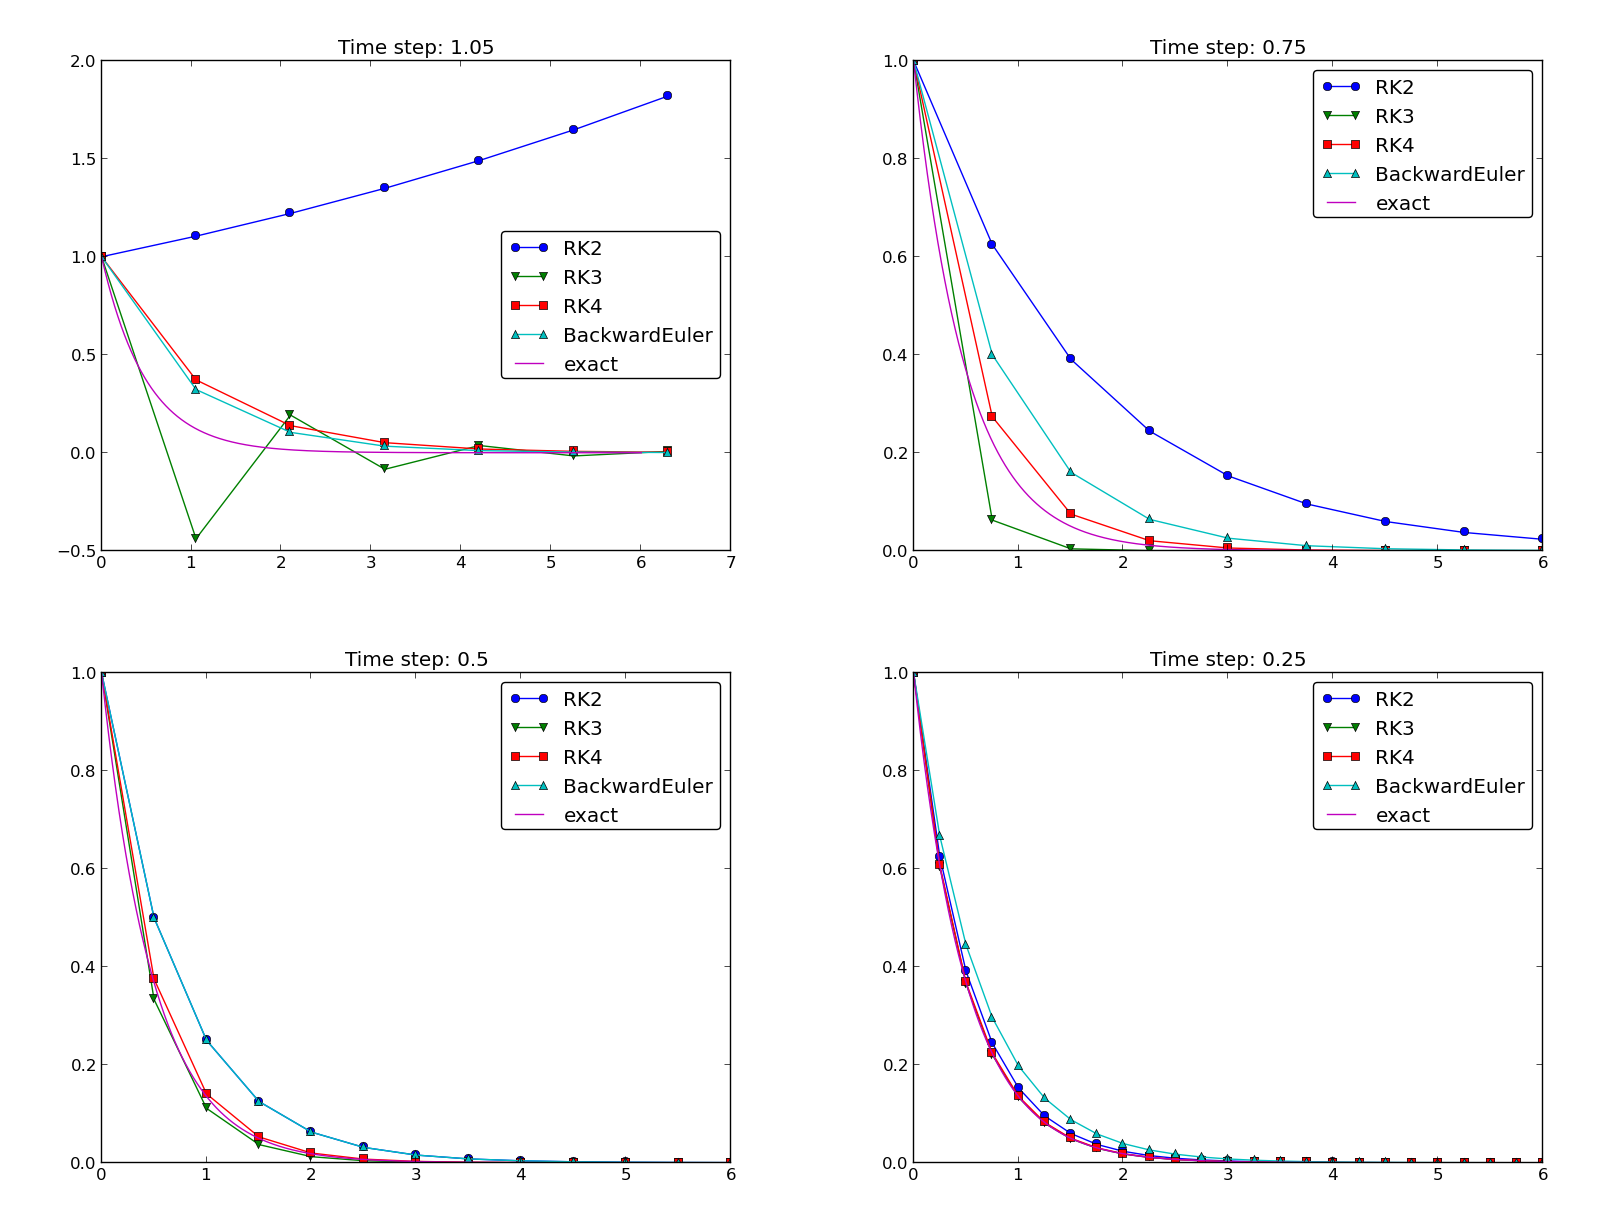
\includegraphics[width=1.1\linewidth]{fig-genz/decay_odespy1_png.png}}
  \caption{
  Behavior of different schemes for the decay equation. \label{decay:odespy:fig1}
  }
\end{figure}
%\clearpage % flush figures decay:odespy:fig1



The runs in Figure~\ref{decay:odespy:fig1}
and other experiments reveal that the 2nd-order Runge-Kutta
method (\texttt{RK2}) is unstable for $\Delta t>1$ and decays slower than the
Backward Euler scheme for large and moderate $\Delta t$ (see Exercise~\ref{decay:exer:RK2:Taylor:analysis} for an analysis).  However, for
fine $\Delta t = 0.25$ the 2nd-order Runge-Kutta method approaches
the exact solution faster than the Backward Euler scheme.  That is,
the latter scheme does a better job for larger $\Delta t$, while the
higher order scheme is superior for smaller $\Delta t$. This is a
typical trend also for most schemes for ordinary and partial
differential equations.

The 3rd-order Runge-Kutta method (\texttt{RK3}) also has artifacts in the form
of oscillatory behavior for the larger $\Delta t$ values, much
like that of the Crank-Nicolson scheme. For finer $\Delta t$,
the 3rd-order Runge-Kutta method converges quickly to the exact
solution.

The 4th-order Runge-Kutta method (\texttt{RK4}) is slightly inferior
to the Backward Euler scheme on the coarsest mesh, but is then
clearly superior to all the other schemes. It is definitely the
method of choice for all the tested schemes.


\paragraph{Remark about using the $\theta$-rule in Odespy.}
The Odespy package assumes that the ODE is written as $u^{\prime}=f(u,t)$ with
an $f$ that is possibly nonlinear in $u$. The $\theta$-rule for
$u^{\prime}=f(u,t)$ leads to
\[ u^{n+1} = u^{n} + \Delta t\left(\theta f(u^{n+1}, t_{n+1})
+ (1-\theta) f(u^{n}, t_{n})\right),\]
which is a \emph{nonlinear equation} in $u^{n+1}$. Odespy's implementation
of the $\theta$-rule (\texttt{ThetaRule}) and the specialized Backward Euler
(\texttt{BackwardEuler}) and Crank-Nicolson (\texttt{CrankNicolson}) schemes
must invoke iterative methods for
solving the nonlinear equation in $u^{n+1}$. This is done even when
$f$ is linear in $u$, as in the model problem $u^{\prime}=-au$, where we can
easily solve for $u^{n+1}$ by hand.  Therefore, we need to specify
use of Newton's method to solve the equations.
(Odespy allows other methods than Newton's to be used, for instance
Picard iteration, but that method is not suitable. The reason is that it
applies the Forward Euler scheme to generate a start value for
the iterations. Forward Euler may give very wrong solutions
for large $\Delta t$ values. Newton's method, on the other hand,
is insensitive to the start value in \emph{linear problems}.)


\subsection{Example: Adaptive Runge-Kutta methods}
\label{decay:fd2:adaptiveRK}

\index{adaptive time stepping}

Odespy also offers solution methods that can adapt the size of $\Delta t$
with time to match a desired accuracy in the solution. Intuitively,
small time steps will be chosen in areas where the solution is changing
rapidly, while larger time steps can be used where the solution
is slowly varying. Some kind of \emph{error estimator} is used to
adjust the next time step at each time level.

\index{ode45@{\rm\texttt{ode45}}} \index{Dormand-Prince Runge-Kutta 4-5 method}

A very popular adaptive method for solving ODEs is the Dormand-Prince
Runge-Kutta method of order 4 and 5. The 5th-order method is used as a
reference solution and the difference between the 4th- and 5th-order
methods is used as an indicator of the error in the numerical
solution.  The Dormand-Prince method is the default choice in MATLAB's
widely used \texttt{ode45} routine.

We can easily set up Odespy to use the Dormand-Prince method and
see how it selects the optimal time steps. To this end, we request
only one time step from $t=0$ to $t=T$ and ask the method to
compute the necessary non-uniform time mesh to meet a certain
error tolerance. The code goes like

\begin{pro}{cbg_blue1}{bar_blue1}\begin{Verbatim}[numbers=none,fontsize=\fontsize{9pt}{9pt},baselinestretch=0.95,xleftmargin=2mm]
import odespy
import numpy as np
import decay_mod
import sys
#import matplotlib.pyplot as plt
import scitools.std as plt

def f(u, t):
    return -a*u

def u_exact(t):
    return I*np.exp(-a*t)

I = 1; a = 2; T = 5
tol = float(sys.argv[1])
solver = odespy.DormandPrince(f, atol=tol, rtol=0.1*tol)

Nt = 1  # just one step - let the scheme find its intermediate points
t_mesh = np.linspace(0, T, Nt+1)
t_fine = np.linspace(0, T, 10001)

solver.set_initial_condition(I)
u, t = solver.solve(t_mesh)

# u and t will only consist of [I, u^Nt] and [0,T]
# solver.u_all and solver.t_all contains all computed points
plt.plot(solver.t_all, solver.u_all, 'ko')
plt.hold('on')
plt.plot(t_fine, u_exact(t_fine), 'b-')
plt.legend(['tol=%.0E' % tol, 'exact'])
plt.savefig('tmp_odespy_adaptive.png')
plt.show()
\end{Verbatim}
\end{pro}
\noindent

Running four cases with tolerances $10^{-1}$, $10^{-3}$, $10^{-5}$,
and $10^{-7}$, gives the results in Figure~\ref{decay:odespy:fig2}.
Intuitively, one would expect denser points in the beginning of
the decay and larger time steps when the solution flattens out.


\begin{figure}[!ht]  % decay:odespy:fig2
  \centerline{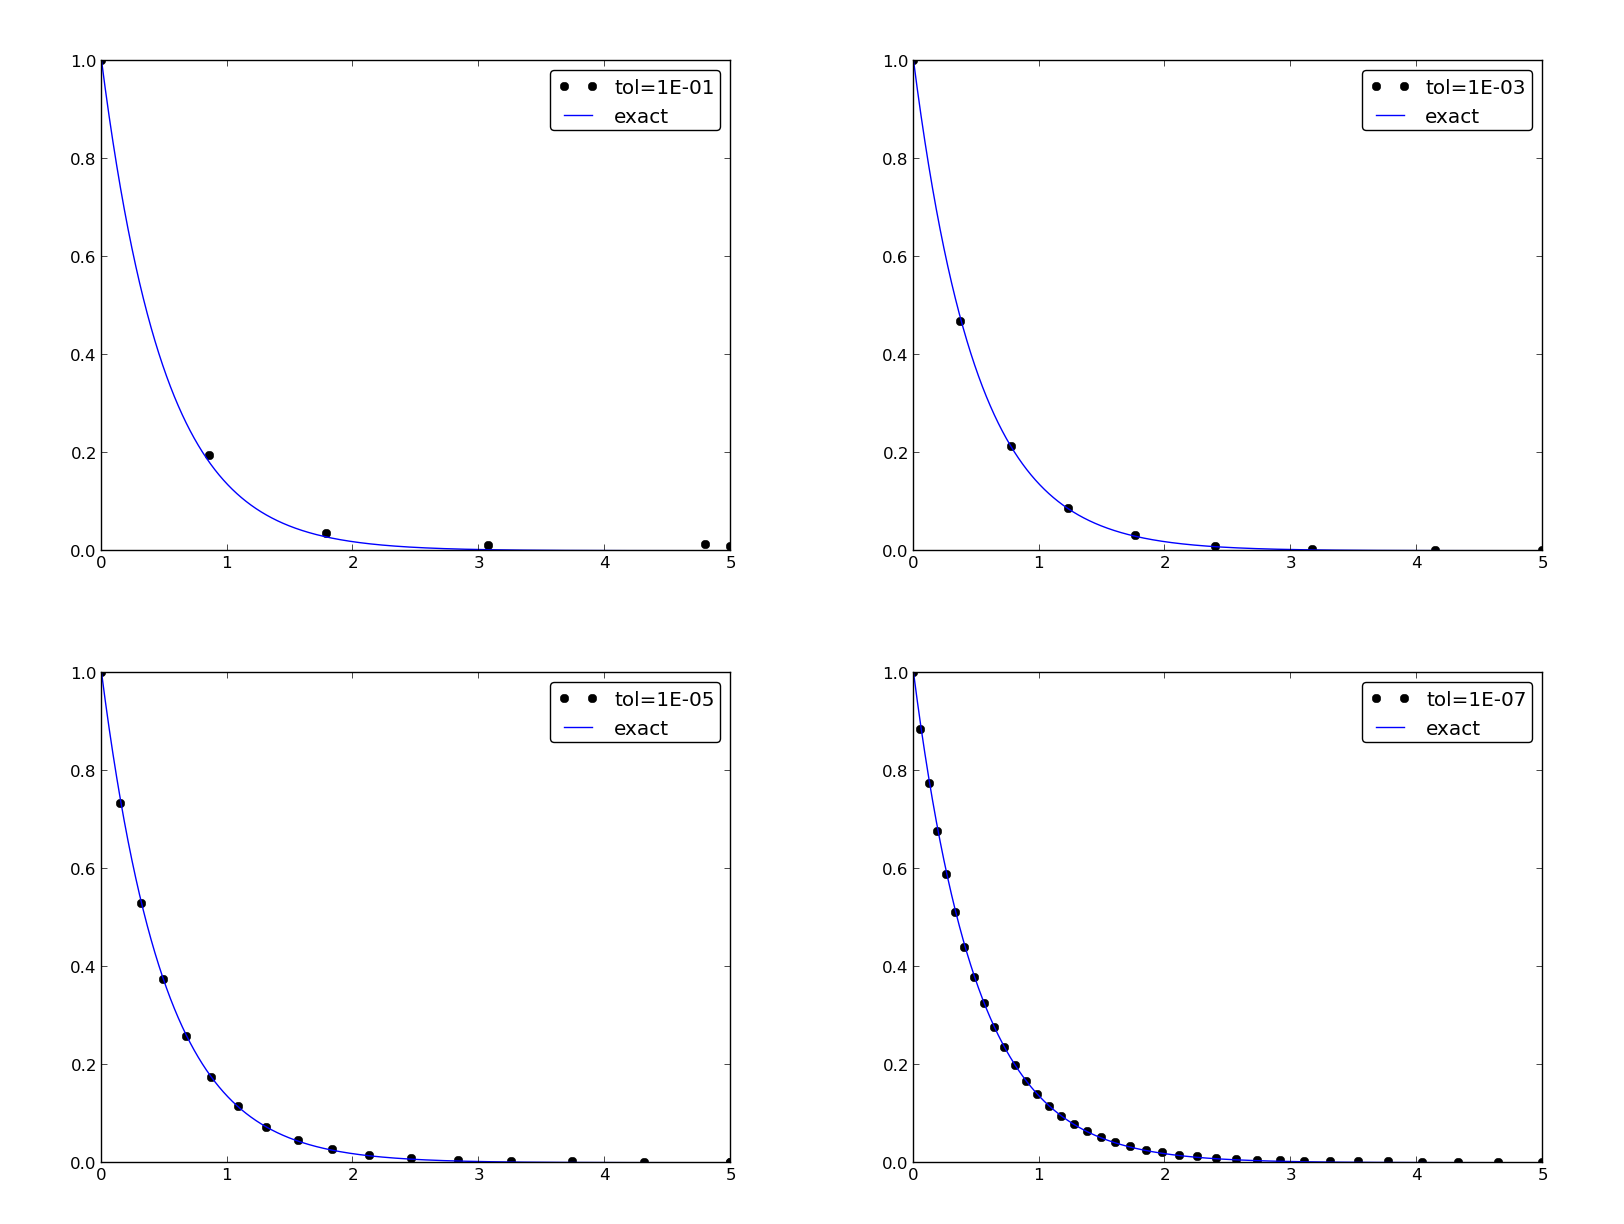
\includegraphics[width=1.2\linewidth]{fig-genz/decay_DormandPrince_adaptivity.png}}
  \caption{
  Choice of adaptive time mesh by the Dormand-Prince method for different tolerances. \label{decay:odespy:fig2}
  }
\end{figure}
%\clearpage % flush figures decay:odespy:fig2




\section{Exercises}



% --- begin exercise ---
\begin{doconceexercise}
\refstepcounter{doconceexercisecounter}

\subsection*{Exercise \thedoconceexercisecounter: Experiment with precision in tests and the size of $u$}
\addcontentsline{loe}{doconceexercise}{Exercise \thedoconceexercisecounter: Experiment with precision in tests and the size of $u$}

\label{decay:fd2:exer:precision}

It is claimed in Section~\ref{decay:MMS} that most numerical methods will
reproduce a linear exact solution to machine precision. Test this
assertion using the test function \Verb!test_linear_solution! in the
\href{{http://tinyurl.com/ofkw6kc/genz/decay_vc.py}}{\nolinkurl{decay_vc.py}} program.
Vary the parameter \texttt{c} from very small, via \texttt{c=1} to many larger values,
and print out the maximum difference between the numerical solution
and the exact solution. What is the relevant value of the tolerance
in the float comparison in each case?


% removed !bsol ... !esol environment (because of the command-line option --without_solutions)
\noindent Filename: \Verb!test_precision!.

\end{doconceexercise}
% --- end exercise ---




% --- begin exercise ---
\begin{doconceexercise}
\refstepcounter{doconceexercisecounter}

\subsection*{Exercise \thedoconceexercisecounter: Implement the 2-step backward scheme}
\addcontentsline{loe}{doconceexercise}{Exercise \thedoconceexercisecounter: Implement the 2-step backward scheme}

\label{decay:fd2:exer:bw2}

Implement the 2-step backward method (\ref{decay:fd2:bw:2step}) for the
model $u^{\prime}(t) = -a(t)u(t) + b(t)$, $u(0)=I$.  Allow the first step to
be computed by either the Backward Euler scheme or the Crank-Nicolson
scheme. Verify the implementation by choosing $a(t)$ and $b(t)$ such
that the exact solution is linear in $t$ (see Section~\ref{decay:MMS}). Show mathematically that a linear solution is indeed a
solution of the discrete equations.

Compute convergence rates (see Section~\ref{decay:convergence:rate}) in
a test case using $a=\hbox{const}$ and $b=0$, where we easily have an exact
solution, and determine if the choice of a first-order scheme
(Backward Euler) for the first step has any impact on the overall
accuracy of this scheme. The expected error goes like $\Oof{\Delta t^2}$.
\noindent Filename: \Verb!decay_backward2step!.

\end{doconceexercise}
% --- end exercise ---




% --- begin exercise ---
\begin{doconceexercise}
\refstepcounter{doconceexercisecounter}

\subsection*{Exercise \thedoconceexercisecounter: Implement the 2nd-order Adams-Bashforth scheme}
\addcontentsline{loe}{doconceexercise}{Exercise \thedoconceexercisecounter: Implement the 2nd-order Adams-Bashforth scheme}

\label{decay:fd2:exer:AB2}

Implement the 2nd-order Adams-Bashforth method (\ref{decay:fd2:AB2})
for the decay problem $u^{\prime}=-a(t)u + b(t)$, $u(0)=I$, $t\in (0, T]$.
Use the Forward Euler method for the first step such that the overall
scheme is explicit. Verify the implementation using an exact
solution that is linear in time.
Analyze the scheme by searching for solutions $u^n=A^n$ when $a=\hbox{const}$
and $b=0$. Compare this second-order scheme to the Crank-Nicolson scheme.
\noindent Filename: \Verb!decay_AdamsBashforth2!.

\end{doconceexercise}
% --- end exercise ---




% --- begin exercise ---
\begin{doconceexercise}
\refstepcounter{doconceexercisecounter}

\subsection*{Exercise \thedoconceexercisecounter: Implement the 3rd-order Adams-Bashforth scheme}
\addcontentsline{loe}{doconceexercise}{Exercise \thedoconceexercisecounter: Implement the 3rd-order Adams-Bashforth scheme}

\label{decay:fd2:exer:AB3}

Implement the 3rd-order Adams-Bashforth method (\ref{decay:fd2:AB3})
for the decay problem $u^{\prime}=-a(t)u + b(t)$, $u(0)=I$, $t\in (0, T]$.
Since the scheme is explicit, allow it to be started by two steps with
the Forward Euler method.  Investigate experimentally the case where
$b=0$ and $a$ is a constant: Can we have oscillatory solutions for
large $\Delta t$?
\noindent Filename: \Verb!decay_AdamsBashforth3!.

\end{doconceexercise}
% --- end exercise ---




% --- begin exercise ---
\begin{doconceexercise}
\refstepcounter{doconceexercisecounter}

\subsection*{Exercise \thedoconceexercisecounter: Analyze explicit 2nd-order methods}
\addcontentsline{loe}{doconceexercise}{Exercise \thedoconceexercisecounter: Analyze explicit 2nd-order methods}

\label{decay:exer:RK2:Taylor:analysis}

Show that the schemes (\ref{decay:fd2:RK2:s2}) and
(\ref{decay:fd2:Taylor2}) are identical in the case $f(u,t)=-a$, where
$a>0$ is a constant. Assume that the numerical solution reads
$u^n=A^n$ for some unknown amplification factor $A$ to be determined.
Find $A$ and derive stability criteria. Can the scheme produce
oscillatory solutions of $u^{\prime}=-au$? Plot the numerical and exact
amplification factor.
\noindent Filename: \Verb!decay_RK2_Taylor2!.

\end{doconceexercise}
% --- end exercise ---




% --- begin exercise ---
\begin{doconceexercise}
\refstepcounter{doconceexercisecounter}

\subsection*{Project \thedoconceexercisecounter: Implement and investigate the Leapfrog scheme}
\addcontentsline{loe}{doconceexercise}{Project \thedoconceexercisecounter: Implement and investigate the Leapfrog scheme}

\label{decay:fd2:exer:leapfrog1}

A Leapfrog scheme
for the ODE $u^{\prime}(t) = -a(t)u(t) + b(t)$ is defined by

\begin{equation}
\lbrack D_{2t}u = -au+b\rbrack^n\tp
\label{decay:fd2:exer:leapfrog1:scheme}
\end{equation}
A separate method is needed to compute $u^1$. The Forward Euler
scheme is a possible candidate.


\subex{a)}
Implement the Leapfrog scheme for the model equation.
Plot the solution in the case $a=1$, $b=0$, $I=1$,
$\Delta t = 0.01$, $t\in [0,4]$. Compare with the exact
solution $\uex(t)=e^{-t}$.

\subex{b)}
Show mathematically that a linear solution in $t$ fulfills the
Forward Euler scheme for the first step and the Leapfrog scheme
for the subsequent steps. Use this linear solution to verify
the implementation, and automate the verification through a test
function.

% --- begin hint in exercise ---

\paragraph{Hint.}
It can be wise to automate the calculations such that it is easy to
redo the calculations for other types of solutions. Here is
a possible \texttt{sympy} function that takes a symbolic expression \texttt{u}
(implemented as a Python function of \texttt{t}), fits the \texttt{b} term, and
checks if \texttt{u} fulfills the discrete equations:

\begin{cod}{cbg_blue1}\begin{Verbatim}[numbers=none,fontsize=\fontsize{9pt}{9pt},baselinestretch=0.95,xleftmargin=2mm]
import sympy as sym

def analyze(u):
    t, dt, a = sym.symbols('t dt a')

    print 'Analyzing u_e(t)=%s' % u(t)
    print 'u(0)=%s' % u(t).subs(t, 0)

    # Fit source term to the given u(t)
    b = sym.diff(u(t), t) + a*u(t)
    b = sym.simplify(b)
    print 'Source term b:', b

    # Residual in discrete equations; Forward Euler step
    R_step1 = (u(t+dt) - u(t))/dt + a*u(t) - b
    R_step1 = sym.simplify(R_step1)
    print 'Residual Forward Euler step:', R_step1

    # Residual in discrete equations; Leapfrog steps
    R = (u(t+dt) - u(t-dt))/(2*dt) + a*u(t) - b
    R = sym.simplify(R)
    print 'Residual Leapfrog steps:', R

def u_e(t):
    return c*t + I

analyze(u_e)
# or short form: analyze(lambda t: c*t + I)
\end{Verbatim}
\end{cod}
\noindent

% --- end hint in exercise ---

\subex{c)}
Show that a second-order polynomial in $t$ cannot be a solution of the discrete
equations. However, if a Crank-Nicolson scheme is used for the first
step, a second-order polynomial solves the equations exactly.


\subex{d)}
Create a manufactured solution $u(t)=\sin(t)$ for the ODE
$u^{\prime}=-au+b$.
Compute the convergence rate of the Leapfrog scheme using this
manufactured solution. The expected convergence rate of the
Leapfrog scheme is $\Oof{\Delta t^2}$. Does the use of a
1st-order method for the first step impact the convergence rate?

% A possible test case is
% $u^{\prime}=-au + b$, $u(0)=0$, where $\uex(t)=b/a + (I - b/a)e^{-at}$ if
% $a$ and $b$ are constants.

\subex{e)}
Set up a set of experiments to demonstrate that the Leapfrog scheme
(\ref{decay:fd2:exer:leapfrog1:scheme}) is associated with numerical artifacts
(instabilities). Document the main results from this investigation.

\subex{f)}
Analyze and explain the
instabilities of the Leapfrog scheme (\ref{decay:fd2:exer:leapfrog1:scheme}):

\begin{enumerate}
\item Choose $a=\mbox{const}$ and $b=0$. Assume that an exact solution
   of the discrete equations has
   the form $u^n=A^n$, where $A$ is an amplification factor to
   be determined. Derive an equation for $A$ by inserting $u^n=A^n$
   in the Leapfrog scheme.

\item Compute $A$ either by hand and/or with the aid of \texttt{sympy}.
   The polynomial for $A$ has two roots, $A_1$ and $A_2$. Let
   $u^n$ be a linear combination $u^n=C_1A_1^n + C_2A_2^n$.

\item Show that one of the roots is the reason for instability.

\item Compare $A$ with the exact expression, using a Taylor series approximation.

\item How can $C_1$ and $C_2$ be determined?
\end{enumerate}

\noindent
\subex{g)}
Since the original Leapfrog scheme is unconditionally unstable as time
grows, it demands some stabilization.  This can be done by filtering,
where we first find $u^{n+1}$ from the original Leapfrog scheme and
then replace $u^{n}$ by $u^n + \gamma (u^{n-1} - 2u^n +
u^{n+1})$, where $\gamma$ can be taken as 0.6.  Implement the filtered
Leapfrog scheme and check that it can handle tests where the original
Leapfrog scheme is unstable.


\noindent Filename: \Verb!decay_leapfrog!.

\end{doconceexercise}
% --- end exercise ---




% --- begin exercise ---
\begin{doconceexercise}
\refstepcounter{doconceexercisecounter}

\subsection*{Problem \thedoconceexercisecounter: Make a unified implementation of many schemes}
\addcontentsline{loe}{doconceexercise}{Problem \thedoconceexercisecounter: Make a unified implementation of many schemes}

\label{decay:fd2:exer:uni}

Consider the linear ODE problem $u^{\prime}(t)=-a(t)u(t) + b(t)$, $u(0)=I$.
Explicit schemes for this problem can be written in the general form
\begin{equation}
u^{n+1} = \sum_{j=0}^m c_ju^{n-j},
\label{decay:analysis:exer:sumcj}
\end{equation}
for some choice of $c_0,\ldots,c_m$.
Find expressions for the $c_j$ coefficients in case of the
$\theta$-rule, the three-level backward scheme,
the Leapfrog scheme, the 2nd-order Runge-Kutta method,
and the 3rd-order Adams-Bashforth scheme.

Make a class \texttt{ExpDecay} that implements the
general updating formula (\ref{decay:analysis:exer:sumcj}).
The formula cannot be applied for $n < m$, and for those $n$ values, other
schemes must be used. Assume for simplicity that we just
repeat Crank-Nicolson steps until (\ref{decay:analysis:exer:sumcj}) can be used.
Use a subclass
to specify the list $c_0,\ldots,c_m$ for a particular method, and
implement subclasses for all the mentioned schemes.
Verify the implementation by testing with a linear solution, which should
be exactly reproduced by all methods.
\noindent Filename: \Verb!decay_schemes_unified!.

\end{doconceexercise}
% --- end exercise ---


% !split
\chapter{Models}
\label{decay:app}

This chapter presents many mathematical models that all end up with
ODEs of the type $u^{\prime}=-au+b$.  The applications are taken from
biology, finance, and physics, and cover population growth or decay,
interacting predator-prey populations, compound interest and
inflation, radioactive decay, chemical and biochemical reaction,
spreading of diseases, cooling of objects, compaction of geological
media, pressure variations in the atmosphere, viscoelastic response in
materials, and air resistance on falling or rising bodies.

Before we turn to the applications, however, we take a brief look at
the technique of scaling, which is so useful in many applications.


\section{Scaling}
\label{decay:app:scaling}

Real applications of a model $u^{\prime}=-au+b$ will often involve a lot
of parameters in the expressions for $a$ and $b$. It can be quite
a challenge to find relevant values of all parameters. In simple
problems, however, it turns out that it is not always necessary
to estimate all parameters because we can lump them into one or
a few \emph{dimensionless} numbers by using a very attractive technique
called scaling. It simply means to stretch the $u$ and $t$ axis
in the present problem - and suddenly all parameters in the problem
are lumped into one parameter if $b\neq 0$ and no parameter when $b=0$!

\subsection{Dimensionless variables}

Scaling means that we introduce a new function $\bar u(\bar t)$,
with

\[ \bar u = \frac{u - u_m}{u_c},\quad \bar t = \frac{t}{t_c},\]
where $u_m$ is a characteristic value of $u$, $u_c$ is a characteristic
size of the range of $u$ values, and $t_c$ is a characteristic
size of the range of $t$ where $u$ shows significant variation.
Choosing $u_m$, $u_c$, and $t_c$ is not always easy and is often an art
in complicated problems. We just state one choice first:

\[ u_c = I,\quad u_m = b/a,\quad t_c = 1/a\tp\]
Inserting $u=u_m + u_c\bar u$ and $t=t_c\bar t$ in the problem
$u^{\prime}=-au + b$, assuming $a$ and $b$ are constants, results (after some
algebra) in the \emph{scaled problem}

\[ \frac{d\bar u}{d\bar t} = -\bar u,\quad \bar u(0)=1 - \beta,\]
where

\[ \beta = \frac{b}{Ia}\tp\]

\subsection{Dimensionless numbers}

The parameter $\beta$ is a dimensionless number. From the equation we
see that $b$ must have the same unit as the term $au$. The initial
condition $I$ must have the same unit as $u$, so $Ia$ has the same
unit as $b$, making the fraction $b/(Ia)$ dimensionless.

An important observation is that $\bar u$ depends on $\bar t$
and $\beta$.
That is, only the special combination of $b/(Ia)$ matters, not what
the individual values of $b$, $a$, and $I$ are. The original unscaled
function $u$ depends on $t$, $b$, $a$, and $I$.

A second observation is striking: if $b=0$, the scaled problem is
independent of $a$ and $I$! In practice this means that we can perform
a single numerical simulation of the scaled problem and recover the
solution of any problem for a given $a$ and $I$ by stretching the axis
in the plot: $u=I\bar u$ and $t =\bar t/a$.  For $b\neq 0$, we
simulate the scaled problem for a few $\beta$ values and recover the
physical solution $u$ by translating and stretching the $u$ axis and
stretching the $t$ axis.

In general, scaling combines the parameters in a problem to a set
of dimensionless parameters. The number of dimensionless parameters is
usually much smaller than the number of original parameters.
Section~\ref{decay:app:drag} presents an example where 11 parameters
are reduced to one!

\subsection{A scaling for vanishing initial condition}

The scaling breaks down if $I=0$. In that case we may choose $u_m=0$,
$u_c=b/a$, and $t_c=1/b$, resulting in a slightly different scaled problem:

\[ \frac{d\bar u}{d\bar t} = 1 -\bar u,\quad \bar u(0)=0\tp\]
As with $b=0$, the case $I=0$ has a scaled problem with no physical
parameters!

It is common to drop the bars after scaling and write the scaled
problem as $u^{\prime}=-u$, $u(0)=1-\beta$, or $u^{\prime}=1-u$, $u(0)=0$.
Any implementation of the problem $u^{\prime}=-au+b$, $u(0)=I$, can be
reused for the scaled problem by setting $a=1$, $b=0$, and $I=1-\beta$
in the code, if $I\neq 0$, or one sets
$a=1$, $b=1$, and $I=0$ when the physical $I$ is zero.
Falling bodies in fluids, as described in Section~\ref{decay:app:drag},
involves $u^{\prime}=-au+b$ with seven physical parameters. All these vanish
in the scaled version of the problem if we start the motion from rest!

Many more details about scaling are presented in the author's book
\emph{Scaling of Differential Equations} \cite{Langtangen_scaling}.

\section{Evolution of a population}
\label{decay:app:pop}

\index{population dynamics}

\subsection{Exponential growth}
\label{decay:app:pop:exp}

Let $N$ be the number of individuals in a population occupying some
spatial domain.  Despite $N$ being an integer in this problem, we
shall compute with $N$ as a real number and view $N(t)$ as a
continuous function of time.  The basic model assumption is that in a
time interval $\Delta t$ the number of newcomers to the populations
(newborns) is proportional to $N$, with proportionality constant $\bar
b$. The amount of newcomers will increase the population and result in

\[ N(t+\Delta t) = N(t) + \bar bN(t)\tp  \]
It is obvious that a long time interval $\Delta t$ will result in
more newcomers and hence a larger $\bar b$. Therefore, we introduce
$b=\bar b/\Delta t$: the number of newcomers per unit time and per
individual. We must then multiply $b$ by the length of the time
interval considered and by the population size to get the
total number of new individuals, $b\Delta t N$.

If the number of removals from the population (deaths) is also
proportional to $N$, with proportionality constant $d\Delta t$,
the population evolves according to
\[ N(t+\Delta t) = N(t) + b\Delta t N(t) - d\Delta t N(t)\tp  \]
Dividing by $\Delta t$ and letting $\Delta t \rightarrow 0$,
we get the ODE

\begin{equation}
N^{\prime} = (b-d)N,\quad N(0)=N_0\tp
\end{equation}
In a population where the death rate ($d$) is larger than
then newborn rate ($b$), $b-d < 0$, and the population experiences
exponential decay rather than exponential growth.

In some populations there is an immigration of individuals into the
spatial domain. With $I$ individuals coming in per time unit,
the equation for the population change becomes

\[ N(t+\Delta t) = N(t) + b\Delta t N(t) - d\Delta t N(t) + \Delta t I\tp  \]
The corresponding ODE reads
\begin{equation}
N^{\prime} = (b-d)N + I,\quad N(0)=N_0
\tp
\end{equation}
Emigration is also modeled by this $I$ term if we just change its sign: $I < 0$.
So, the $I$ term models migration in and out of the domain in general.

Some simplification arises if we introduce a fractional measure
of the population: $u=N/N_0$ and set $r=b-d$. The ODE problem
now becomes

\begin{equation}
u^{\prime} = ru + f,\quad u(0)=1,
\label{decay:app:pop:ueq}
\end{equation}
where $f=I/N_0$ measures the net immigration per time unit as
the fraction of the initial population. Very often, $r$ is approximately
constant, but $f$ is usually a function of time.

\subsection{Logistic growth}
\label{decay:app:pop:log}

\index{logistic model}

The growth rate $r$ of a population decreases if the environment
has limited resources. Suppose the environment can sustain at
most $N_{\max}$ individuals. We may then assume that the growth rate
approaches zero as $N$ approaches $N_{\max}$, i.e., as $u$ approaches
$M=N_{\max}/N_0$. The simplest possible evolution of $r$ is then a
linear function: $r(t)={\varrho}(1-u(t)/M)$, where $\varrho$
is the initial growth rate when the population is small relative to the
maximum size and there is enough resources. Using this $r(t)$ in
(\ref{decay:app:pop:ueq}) results in the \emph{logistic model} for the
evolution of a population (assuming for the moment that $f=0$):
\begin{equation}
u^{\prime} = {\varrho}(1-u/M)u,\quad u(0)=1
\tp
\label{decay:app:pop:logistic}
\end{equation}
Initially, $u$ will grow at rate $\varrho$, but the growth will decay
as $u$ approaches $M$, and then there is no more change in $u$, causing
$u\rightarrow M$ as $t\rightarrow\infty$.
Note that the logistic equation $u^{\prime}={\varrho}(1-u/M)u$ is \emph{nonlinear} because
of the quadratic term $-u^2{\varrho}/M$.

\section{Compound interest and inflation}
\label{decay:app:interest}

Say the annual interest rate is $r$ percent and that the bank
adds the interest once a year to your investment.
If $u^n$ is the investment in year $n$, the investment in year $u^{n+1}$
grows to

\[ u^{n+1} = u^n + \frac{r}{100}u^n
\tp  \]
In reality, the interest rate is added every day. We therefore introduce
a parameter $m$ for the number of periods per year when the interest
is added. If $n$ counts the periods, we have the fundamental model
for compound interest:
\begin{equation}
u^{n+1} = u^n + \frac{r}{100 m}u^n
\tp
\label{decay:app:interest:eq1}
\end{equation}
This model is a \emph{difference equation}, but it can be transformed to a
continuous differential equation through a limit process.
The first step is to derive a formula for the growth of the investment
over a time $t$.
Starting with an investment $u^0$, and assuming that $r$ is constant in time,
we get
\begin{align*}
u^{n+1} &= \left(1 + \frac{r}{100 m}\right)u^{n}\\ 
&= \left(1 + \frac{r}{100 m}\right)^2u^{n-1}\\ 
&\ \ \vdots\\ 
&= \left(1 +\frac{r}{100 m}\right)^{n+1}u^{0}
\end{align*}
Introducing time $t$, which here is a real-numbered counter for years,
we have that $n=mt$, so we can write

\[ u^{mt} = \left(1 + \frac{r}{100 m}\right)^{mt} u^0\tp  \]
The second step is to assume \emph{continuous compounding}, meaning that the
interest is added continuously. This implies $m\rightarrow\infty$, and
in the limit one gets the formula
\begin{equation}
u(t) = u_0e^{rt/100},
\end{equation}
which is nothing but the solution of the ODE problem
\begin{equation}
u^{\prime} = \frac{r}{100}u,\quad u(0)=u_0
\tp
\label{decay:app:interest:eq2}
\end{equation}
This is then taken as the ODE model for compound interest if $r>0$.
However, the reasoning applies equally well to inflation, which is
just the case $r < 0$.
One may also take the $r$ in (\ref{decay:app:interest:eq2})
as the net growth of an investment, where $r$ takes both compound interest
and inflation into account. Note that for real applications we must
use a time-dependent $r$ in (\ref{decay:app:interest:eq2}).


Introducing $a=\frac{r}{100}$, continuous inflation of an initial
fortune $I$ is then
a process exhibiting exponential decay according to
\[ u^{\prime} = -au,\quad u(0)=I\tp  \]

\section{Newton's law of cooling}
\label{decay:app:Newton:cooling}

% \href{{http://web.bham.ac.uk/winterhs/Newton.htm}}{\nolinkurl{http://web.bham.ac.uk/winterhs/Newton.htm}}
% I. Newton, Scala Graduum Caloris, Philosophical Transactions of the Royal Society of London, 1701
% explanation: \href{{http://www.madsci.org/posts/archives/2000-11/973522810.Ph.r.html}}{\nolinkurl{http://www.madsci.org/posts/archives/2000-11/973522810.Ph.r.html}}

When a body at some temperature is placed in a cooling environment,
experience shows that the temperature falls rapidly in the beginning,
and then the change in temperature levels off until the body's
temperature equals that of the surroundings. Newton carried out some
experiments on cooling hot iron and found that the temperature
evolved as a ``geometric progression at times in arithmetic progression'',
meaning that the temperature decayed exponentially.
Later, this result was formulated as a differential equation:
the rate of change of the temperature in a body is proportional to
the temperature difference between the body and its surroundings.
This statement is known as \emph{Newton's law of cooling}, which
mathematically can be expressed as

\begin{equation}
{dT\over dt} = -k(T-T_s),
\label{decay:Newton:cooling}
\end{equation}
where $T$ is the temperature of the body, $T_s$ is the temperature
of the surroundings (which may be time-dependent),
$t$ is time, and $k$ is a positive constant.
Equation (\ref{decay:Newton:cooling}) is primarily viewed as an
empirical law, valid when heat is efficiently convected away
from the surface of the body by a flowing fluid such as air
at constant temperature $T_s$.
The \emph{heat transfer coefficient} $k$ reflects the transfer of
heat from the body to
the surroundings and must be determined from physical experiments.

The cooling law (\ref{decay:Newton:cooling}) needs an initial
condition $T(0)=T_0$.


\section{Radioactive decay}
\label{decay:app:nuclear}

\index{radioactive decay}

An atomic nucleus of an unstable atom may lose energy by emitting
ionizing particles and thereby be transformed to a nucleus with a
different number of protons and neutrons.  This process is known as
\href{{http://en.wikipedia.org/wiki/Radioactive_decay}}{radioactive decay}.
Actually, the process is stochastic when viewed for a single atom,
because it is impossible to predict exactly when a particular atom
emits a particle. Nevertheless, with a large number of atoms, $N$, one
may view the process as deterministic and compute the mean behavior of
the decay. Below we reason intuitively about an ODE for the mean
behavior. Thereafter, we show mathematically that a detailed stochastic model
for single atoms leads to the same mean behavior.

\subsection{Deterministic model}

Suppose at time $t$, the number of the original atom type is $N(t)$.
A basic model assumption is that the transformation of the atoms of the original
type in a small time interval $\Delta t$ is proportional to
$N$, so that

\[ N(t+\Delta t) = N(t) - a\Delta t N(t),\]
where $a>0$ is a constant. The proportionality factor is $a\Delta t$, i.e.,
proportional to $\Delta t$ since a longer time interval will produce more
transformations.
We can introduce $u=N(t)/N(0)$, divide by
$\Delta t$, and let $\Delta t\rightarrow 0$:

\[ \lim_{r\rightarrow 0}
N_0\frac{u(t+\Delta t) - u(t)}{\Delta t} = - a N_0 u(t)\tp\]
The left-hand side is the derivative of $u$. Dividing by the $N_0$ gives
the following ODE for $u$:

\begin{equation}
u^{\prime} = -au,\quad u(0)=1
\tp
\end{equation}

The parameter $a$ can for a given nucleus be expressed through the
\emph{half-life} $t_{1/2}$, which is the time taken for the decay to reduce the
initial amount by one half, i.e., $u(t_{1/2}) = 0.5$.
With $u(t)=e^{-at}$, we get $t_{1/2}=a^{-1}\ln 2$ or $a=\ln 2/t_{1/2}$.

% \href{{http://en.wikipedia.org/wiki/Exponential_decay}}{\nolinkurl{http://en.wikipedia.org/wiki/Exponential_decay}}

\subsection{Stochastic model}

Originally, we have $N_0$ atoms. Up to some particular time $t$, each
atom may either have decayed or not. If not, they have ``survived''.
We want to count how many original
atoms that have survived.
The survival of a single atom at time $t$ is a random event. Since there
are only two outcomes, survival or decay, we have a
\href{{http://en.wikipedia.org/wiki/Bernoulli_trial}}{Bernoulli trial}.
Let $p$ be the
probability of survival (implying that the probability of decay
is $1-p$). If each atom survives independently of
the others, and the probability of survival is the same for every
atom, we have $N_0$ Bernoulli trials, known as
a \emph{binomial experiment} from probability theory.
The probability $P(N)$ that $N$ out
of the $N_0$ atoms have survived at time $t$ is then given by the
famous \emph{binomial distribution}

\[ P(N) = \frac{N_0!}{N! (N_0-N)!}p^N (1-p)^{N_0-N}\tp \]
The mean (or expected) value $\E{P}$ of $P(N)$ is known to be $N_0p$.

It remains to estimate $p$. Let the interval $[0,t]$ be divided into $m$
small subintervals of length $\Delta t$. We make the assumption that
the probability of decay of a single atom in an interval of length $\Delta t$
is $\tilde p$, and that this probability is proportional to $\Delta t$:
$\tilde p = \lambda\Delta t$ (it sounds natural that the probability
of decay increases with $\Delta t$). The corresponding probability of survival
is $1-\lambda\Delta t$. Believing that $\lambda$ is independent
of time, we have, for each interval of length $\Delta t$,
a Bernoulli trial: the atom either survives or
decays in that interval. Now, $p$ should be the probability that the atom
survives in all the intervals, i.e., that we have $m$ successful
Bernoulli trials in a row and therefore

\[ p = (1-\lambda\Delta t)^m\tp\]
The expected number of atoms of the original type at time $t$ is

\begin{equation}
\E{P} = N_0p = N_0(1-\lambda\Delta t)^m,\quad m=t/\Delta t\tp
\end{equation}

To see the relation between the two types of Bernoulli trials and the
ODE above, we go to the limit $\Delta t\rightarrow 0$, $m\rightarrow\infty$.
It is possible to show that

\[ p = \lim_{m\rightarrow\infty} (1-\lambda\Delta t)^m
= \lim_{m\rightarrow\infty} \left(1-\lambda\frac{t}{m}\right)^m = e^{-\lambda t}
\]
This is the famous exponential waiting time (or arrival time) distribution for a
Poisson process in probability theory (obtained here, as often done, as
the limit of a binomial experiment). The probability of decay, or more
precisely that at least one atom has undergone a transition, is
$1-p= 1-e^{-\lambda t}$. This is the
\href{{http://en.wikipedia.org/wiki/Exponential_distribution}}{exponential distribution}.
The limit means that $m$ is very
large, hence $\Delta t$ is very small, and $\tilde p=\lambda\Delta t$
is very small since the intensity of the events, $\lambda$, is assumed
finite. This situation corresponds to a very small probability
that an atom will decay in a very short time interval, which is a
reasonable model.
The same model occurs in lots of different applications, e.g.,
when waiting for a taxi, or when finding defects along a rope.

\subsection{Relation between stochastic and deterministic models}

With $p=e^{-\lambda t}$ we get the expected number of original atoms
at $t$ as $N_0p=N_0e^{-\lambda t}$, which is exactly the solution of
the ODE model $N^{\prime}=-\lambda N$. This also gives an interpretation
of $a$ via $\lambda$ or vice versa. Our important finding here
is that the ODE model
captures the mean behavior of the underlying stochastic model. This
is, however, not always the common relation between microscopic stochastic
models and macroscopic ``averaged'' models.

Also of interest, is that a Forward Euler discretization of
$N^{\prime}=-\lambda N$, $N(0)=N_0$, gives $N^m = N_0(1-\lambda\Delta t)^m$
at time $t_m=m\Delta t$, which is exactly the
expected value of the stochastic experiment with $N_0$ atoms
and $m$ small intervals of length $\Delta t$, where each atom can
decay with probability $\lambda\Delta t$ in an interval.

A fundamental question is how accurate the ODE model is. The underlying
stochastic model fluctuates around its expected value. A measure
of the fluctuations is the standard deviation of the binomial experiment with
$N_0$ atoms, which can be shown to be $\Std{P}=\sqrt{N_0p(1-p)}$. Compared
to the size of the expectation, we get
the normalized standard deviation

\[ \frac{\sqrt{\Var{P}}}{\E{P}} = N_0^{-1/2}\sqrt{p^{-1}-1}
= N_0^{-1/2}\sqrt{(1-e^{-\lambda t})^{-1}-1}\approx
(N_0\lambda t)^{-1/2},
\]
showing that the normalized fluctuations are very small if $N_0$ is
very large, which is usually the case.

\subsection{Generalization of the radioactive decay modeling}
\label{decay:app:waitingtime}

The modeling in Section~\ref{decay:app:nuclear} is in fact very
general, despite a focus on a particular physical process. We may
instead of atoms and decay speak about a set of \emph{items}, where each
item can undergo a stochastic \emph{transition} from one state to
another. In Section~\ref{decay:app:kinetics} the item is a molecule and
the transition is a chemical reaction, while in Section~\ref{decay:app:SIR} the item is an ill person and the transition is
recovering from the illness (or an immune person who loses her
immunity).

From the modeling in Section~\ref{decay:app:nuclear} we can establish
a deterministic model for a large number of items and a stochastic
model for an arbitrary number of items, even a single one.
The stochastic model has a parameter $\lambda$ reflecting the
probability that a transition takes place in a time interval of
unit length (or equivalently, that the probability is $\lambda\Delta t$
for a transition during a time interval of length $\Delta t$).
The probability of making a transition before time $t$ is given by

\[ F(t) = 1- e^{-\lambda t}\tp\]
The corresponding probability density is $f(t)=F'(t)=e^{-\lambda t}$.
The expected value of $F(t)$, i.e., the expected time to transition,
is $\lambda^{-1}$. This interpretation of $\lambda$ makes it easy to
measure its value: just carry out a large number of experiments,
measure the time to transition, and take one over the average of these times as
an estimate of $\lambda$.
The variance is $\lambda^{-2}$.

The deterministic model counts how many items, $N(t)$, that have
undergone the transition (on average), and $N(t)$ is governed by the ODE

\[ N^{\prime} = -\lambda N(t),\quad N(0)=N_0\tp\]


\section{Chemical kinetics}
\label{decay:app:kinetics}

\index{chemical reactions!irreversible}

\subsection{Irreversible reaction of two substances}

Consider two chemical substances, A and B, and a chemical reaction that
turns A into B. In a small time interval, some of the
molecules of type A are transformed into molecules of B. This process is,
from a mathematical modeling point of view, equivalent to the
radioactive decay process described in the previous section. We can
therefore apply the same modeling approach. If $N_A$ is the number of
molecules of substance A, we have that $N_A$ is governed by the
differential equation

\[ \frac{dN_A}{dt} = -kN_A,\]
where (the constant) $k$ is called the \emph{rate constant} of the reaction.
Rather than using the number of molecules, we use the \emph{concentration}
of molecules: $[A](t) = N_A(t)/N_A(0)$.
We see that $d[A]/dt = N_A(0)^{-1} dN_A/dt$.
Replacing $N_A$ by $[A]$ in the equation for $N_A$ leads to the equation
for the concentration $[A]$:

\begin{equation}
\frac{d[A]}{dt} = -k[A],\quad t\in (0,T],\ [A](0)=1, \tp
\label{decay:app:kinetics:irrev:A}
\end{equation}
Since substance A is transformed to substance B, we have that the concentration
of $[B]$ grows by the loss of $[A]$:

\[
\frac{d[B]}{dt} = k[A],\quad [B](0)=0\tp
\]
The mathematical model can either be (\ref{decay:app:kinetics:irrev:A}) or
the system

\begin{align}
\frac{d[A]}{dt} &= -k[A], &t\in (0,T]\\ 
\frac{d[B]}{dt} &= k[A], &t\in (0,T]\\ 
[A](0) &= 1,\\ 
[B](0) &= 0\tp
\end{align}

This reaction is known as a \emph{first-order reaction}, where each molecule of
A makes an independent decision about whether to complete the reaction,
i.e., independent of what happens to any other molecule.

An $n$-th order reaction is modeled by

\begin{align}
\frac{d[A]}{dt} &= -k[A]^n,\\ 
\frac{d[B]}{dt} &= k[A]^n,
\end{align}
for $t\in (0,T]$ with initial conditions $[A](0) = 1$ and
$[B](0) = 0$. Here, $n$ can be a real number,
but is most often an integer. Note that
the sum of the concentrations is constant since

\[ \frac{d[A]}{dt} + \frac{d[B]}{dt} = 0\quad\Rightarrow\quad
[A](t) + [B](t) = \hbox{const} = [A](0) + [B](0) = 1 + 0\tp\]

\index{chemical reactions!reversible}

\subsection{Reversible reaction of two substances}

Let the chemical reaction turn substance A into B and substance B into A.
The rate of change of $[A]$ has then two contributions: a loss $k_A[A]$
and a gain $k_B[B]$:

\begin{equation}
\frac{d[A]}{dt} = -k_A[A] + k_B[B], \quad t\in (0,T],\ [A](0)=A_0\tp
\end{equation}
Similarly for substance B,

\begin{equation}
\frac{d[B]}{dt} = k_A[A] - k_B[B], \quad t\in (0,T],\ [B](0)=B_0\tp
\end{equation}
This time we have allowed for arbitrary initial concentrations.
Again,

\[ \frac{d[A]}{dt} + \frac{d[B]}{dt} = 0\quad\Rightarrow\quad
[A](t) + [B](t) = A_0+B_0\tp\]

\subsection{Irreversible reaction of two substances into a third}

Now we consider two chemical substances, A and B, reacting with each
other and producing a substance C. In a small time interval $\Delta t$,
molecules of type A and B are occasionally colliding, and in some
of the collisions, a chemical reaction occurs, which turns A and B into
a molecule of type C. (More generally, $M_A$ molecules of A and $M_B$
molecules of B react to form $M_C$ molecules of $C$.)
The number of possible pairings, and thereby collisions, of A and B is
$N_AN_B$, where $N_A$ is the number of molecules of A, and $N_B$ is the
number of molecules of B.
A fraction $k$ of these collisions,
$\hat k\Delta t N_AN_B$, features a chemical reaction and produce
$N_C$ molecules of C. The fraction is thought to be proportional to
$\Delta t$: considering a twice as long time interval, twice as many
molecules collide, and twice as many reactions occur.
The increase in molecules of substance C is now found
from the reasoning

\[ N_C(t+\Delta t) = N_C(t) + \hat k\Delta t N_AN_B\tp\]
Dividing by $\Delta t$,

\[ \frac{N_C(t+\Delta t) - N_C(t)}{\Delta t} = \hat k N_AN_B,\]
and letting $\Delta t\rightarrow 0$, gives the differential equation

\[ \frac{dN_C}{dt} = \hat k N_AN_B\tp\]
(This equation is known as the important \href{{https://en.wikipedia.org/wiki/Law_of_mass_action}}{law of mass action} discovered by
the Norwegian scientists Cato M.~Guldberg and Peter Waage.
A more general form of the right-hand side is $\hat kN_A^{\alpha}N_B^{\beta}$.
All the constants $\hat k$, $\alpha$, and $\beta$ must be determined from
experiments.)

Working instead with concentrations, we introduce $[C](t)=N_C(t)/N_C(0)$,
with similar definitions for $[A]$ and $[B]$ we get

\begin{equation}
\frac{d[C]}{dt} = k [A][B]\tp
\end{equation}
The constant $k$ is related to $\hat k$ by $k = \hat k N_A(0)N_B(0)/N_C(0)$.
The gain in C is a loss of A and B:

\begin{align}
\frac{d[A]}{dt} &= -k[A][B],\\ 
\frac{d[B]}{dt} &= -k[A][B]\tp
\end{align}

\subsection{A biochemical reaction}

A common reaction (known as \href{{https://en.wikipedia.org/wiki/Michaelis-Menten_kinetics}}{Michaelis-Menton kinetics}) turns a substrate S into
a product P with aid of an enzyme E. The reaction is a two-stage process:
first S and E reacts to form a complex ES, where the enzyme and substrate
are bound to each other, and then ES is turned into E and P.
In the first stage, S and E react to produce a growth of ES according
to the law of mass action:

\begin{align*}
\frac{d[S]}{dt} &= - k_+[E][S],\\ 
\frac{d[ES]}{dt} &= k_+[E][S]\tp\\ 
\end{align*}
The complex ES reacts and produces the product $P$ at rate
$-k_{v}[ES]$ and E at rate $-k_-[ES]$. The total set of reactions can
then be expressed by

\begin{align}
\frac{d[ES]}{dt} &= k_+[E][S] - k_v[ES] - k_-[ES],
\label{decay:app:MMK:ES1}\\ 
\frac{d[P]}{dt} &= k_v[ES],
\label{decay:app:MMK:P1}\\ 
\frac{d[S]}{dt} &= -k_+[E][S] + k_-[ES],
\label{decay:app:MMK:S1}\\ 
\frac{d[E]}{dt} &= -k_+[E][S] + k_-[ES] + k_v[ES]\tp
\label{decay:app:MMK:E1}
\end{align}
The initial conditions are $[ES](0)=[P](0)=0$, and $[S]=S_0$, $[E]=E_0$.
The constants $k_+$, $k_-$, and $k_v$ must be determined from experiments.

% It is easy to see that $[ES]^{\prime} + [E]^{\prime}=0$, i.e.,
% $[ES] + [E]= E_0=\hbox{const}$. And $[ES] + [S] + [P]$ is constant.

% Dimensionless Michaelis constant: (k_v + k_-)/k_+

\section{Spreading of diseases}
\label{decay:app:SIR}

The modeling of spreading of diseases is very similar to the modeling
of chemical reactions in Section~\ref{decay:app:kinetics}. The field
of epidemiology speaks about susceptibles: people who can get a disease;
infectives: people who are infected and can infect susceptibles; and
recovered: people who have recovered from the disease and
become immune.
Three categories are accordingly defined: S for susceptibles, I for
infectives, and R for recovered. The number in each category is tracked
by the functions $S(t)$, $I(t)$, and $R(t)$.

To model how many people that get infected in a small time interval
$\Delta t$, we reason as with reactions in Section~\ref{decay:app:kinetics}.
The possible number of pairings (``collisions'') between susceptibles
and infected is $SI$. A fraction of these, $\beta\Delta t SI$,
will actually meet and the infected succeed in infecting the susceptible,
where $\beta$ is a parameter to be empirically estimated.
This leads to a loss of susceptibles and a gain of infected:

\begin{align*}
S(t+\Delta t) &= S(t) - \beta\Delta tSI,\\ 
I(t+\Delta t) &= I(t) + \beta\Delta tSI\tp
\end{align*}
In the same time interval, a fraction $\nu\Delta t I$
of the infected is recovered.
It follows from Section~\ref{decay:app:waitingtime}
that the parameter $\nu^{-1}$ is interpreted as the average
waiting time to leave the I category, i.e., the
average length of the disease.
The $\nu \Delta tI$ term is a loss for the I category, but a gain for the R
category:

\begin{align*}
I(t+\Delta t) &= I(t) + \beta\Delta tSI - \nu\Delta t I,
R(t+\Delta t) &= R(t) + \nu\Delta t I\tp
\end{align*}
Dividing these equations by $\Delta t$ and going to the limit
$\Delta t\rightarrow 0$, gives the ODE system

\begin{align}
\frac{dS}{dt} &= -\beta SI,
\label{decay:app:SIR:S}\\ 
\frac{dI}{dt} &=  \beta SI - \nu I,
\label{decay:app:SIR:I}\\ 
\frac{dR}{dt} &= \nu I,
\label{decay:app:SIR:R}
\end{align}
with initial values $S(0)=S_0$, $I(0)=I_0$, and $R(0)=0$.
By adding the equations, we realize that

\[ \frac{dS}{dt}+\frac{dI}{dt}+\frac{dR}{dt}=0\quad\Rightarrow\quad
S+I+R=\hbox{const}=N,\]
where $N$ is the total number in the population under consideration.
This property can be used as a partial verification during simulations.

Equations (\ref{decay:app:SIR:S})-(\ref{decay:app:SIR:R}) are known as
the SIR model in epidemiology. The model can easily be extended to
incorporate vaccination programs, immunity loss after some time, etc.
Typical diseases that can be simulated by the SIR model and its variants
are measles, smallpox, flu, plague, and HIV.

\section{Predator-prey models in ecology}
\label{decay:app:predprey}

\index{Lotka-Volterra model}
\index{predator-prey model}

A model for the interaction of predator and prey species can be based
on reasoning from population dynamics and the SIR model.
Let $H(t)$ be the number of preys in a region, and let $L(t)$
be the number of predators. For example, $H$ may be hares and $L$ lynx,
or rabbits and foxes.

The population of the prey evolves due to births and deaths, exactly
as in a population dynamics model from Section~\ref{decay:app:pop:exp}.
During a time interval $\Delta t$ the increase in the population is
therefore

\[ H(t+\Delta t) - H(t) =  a\Delta t H(t),\]
where $a$ is a parameter to be measured from data.
The increase is proportional to $H$, and the proportionality constant
$a\Delta t$ is proportional to $\Delta t$, because doubling the
interval will double the increase.

However, the prey population has an additional loss because they
are eaten by predators. All the prey and predator animals can form
$LH$ pairs in total (assuming all individuals meet randomly).
A small fraction $b\Delta t$
of such meetings, during a time interval $\Delta t$,
ends up with the predator eating the prey. The increase in the prey
population is therefore adjusted to

\[ H(t+\Delta t) - H(t) =  a\Delta t H(t) - b\Delta t H(t)L(t)\tp\]

The predator population increases as a result of eating preys.
The amount of eaten preys is $b\Delta t LH$, but only a fraction
$d\Delta t LH$ of this amount contributes to increasing the
predator population. In addition, predators die and this loss
is set to $c\Delta t L$. To summarize, the increase in the predator
population is given by

\[ L(t + \Delta t) - L(t) = d\Delta t L(t)H(t) - c\Delta t L(t)\tp\]
Dividing by $\Delta t$ in the equations for $H$ and $L$ and letting
$t\rightarrow 0$ results in

\begin{align*}
\lim_{\Delta t\rightarrow 0}\frac{H(t+\Delta t)-H(t)}{\Delta t}
= H^{\prime}(t) &= aH(t) - bL(t)H(t),\\ 
\lim_{\Delta t\rightarrow 0}\frac{L(t+\Delta t)-L(t)}{\Delta t}
= L^{\prime}(t) &= dL(t)H(t) - cL(t)\tp
\end{align*}
We can simplify the notation to the following two ODEs:

\begin{align}
H^{\prime} &= H(a - bL),
\label{decay:app:predprey:eqH}\\ 
L^{\prime} &= L(dH - c)\tp
\label{decay:app:predprey:eqL}
\end{align}
This is a so-called Lokta-Volterra model. It contains four parameters
that must be estimated from data: $a$, $b$, $c$, and $d$. In addition, two
initial conditions are needed for $H(0)$ and $L(0)$.

\section{Decay of atmospheric pressure with altitude}
\label{decay:app:atm}

% The Barometric Formula
% \href{{http://en.wikipedia.org/wiki/Barometric_formula}}{\nolinkurl{http://en.wikipedia.org/wiki/Barometric_formula}}

\subsection{The general model}

Vertical equilibrium of air in the atmosphere is governed by
the equation

\begin{equation}
\frac{dp}{dz} = -\varrho g
\tp
\label{decay:app:atm:dpdz}
\end{equation}
Here, $p(z)$ is the air pressure, $\varrho$ is the density of
air, and $g=9.807\hbox{ m/s}^2$ is a standard value of
the acceleration of gravity.
(Equation (\ref{decay:app:atm:dpdz}) follows directly from the general
Navier-Stokes equations for fluid motion, with
the assumption that the air does not move.)

The pressure is related to density and temperature through the ideal gas law

\begin{equation}
\varrho = \frac{Mp}{R^*T}, \label{decay:app:atm:rho}
\end{equation}
where $M$ is the molar mass of the Earth's air (0.029 kg/mol),
$R^*$ is the universal
gas constant ($8.314$ Nm/(mol K)), and $T$ is the temperature in Kelvin.
All variables $p$, $\varrho$, and $T$ vary with the height $z$.
Inserting (\ref{decay:app:atm:rho}) in (\ref{decay:app:atm:dpdz}) results
in an ODE with a variable coefficient:

\begin{equation}
\frac{dp}{dz} = -\frac{Mg}{R^*T(z)} p
\label{decay:app:atm:ode}
\thinspace  .
\end{equation}

\subsection{Multiple atmospheric layers}

The atmosphere can be approximately modeled by seven layers.
In each layer, (\ref{decay:app:atm:ode}) is applied with
a linear temperature of the form

\[ T(z) = \bar T_i + L_i(z-h_i),\]
where $z=h_i$ denotes the bottom of layer number $i$,
having temperature $\bar T_i$,
and $L_i$ is a constant in layer number $i$. The table below
lists $h_i$ (m), $\bar T_i$ (K), and $L_i$ (K/m) for the layers
$i=0,\ldots,6$.



{\small   % for Springer style: small table font and more vspace

\vspace{4mm}

\begin{tabular}{lrrr}
\hline
\multicolumn{1}{c}{ $i$ } & \multicolumn{1}{c}{ $h_i$ } & \multicolumn{1}{c}{ $\bar T_i$ } & \multicolumn{1}{c}{ $L_i$ } \\
\hline
0   & 0      & 288        & -0.0065 \\
1   & 11,000 & 216        & 0.0     \\
2   & 20,000 & 216        & 0.001   \\
3   & 32,000 & 228        & 0.0028  \\
4   & 47,000 & 270        & 0.0     \\
5   & 51,000 & 270        & -0.0028 \\
6   & 71,000 & 214        & -0.002  \\
\hline
\end{tabular}

\vspace{4mm}

}


\noindent
For implementation it might be convenient to write (\ref{decay:app:atm:ode})
on the form
\begin{equation}
\frac{dp}{dz} = -\frac{Mg}{R^*(\bar T(z) + L(z)(z-h(z)))} p,
\end{equation}
where $\bar T(z)$, $L(z)$, and $h(z)$ are piecewise constant
functions with values given in the table.
The value of the pressure at the sea level $z=0$, $p_0=p(0)$, is $101325$ Pa.

\subsection{Simplifications}

\paragraph{Constant layer temperature.}
One common simplification is to assume that the temperature is
constant within each layer. This means that $L=0$.

\paragraph{One-layer model.}
Another commonly used approximation is to work with one layer instead of
seven. This \href{{http://en.wikipedia.org/wiki/Density_of_air}}{one-layer model}
is based on $T(z)=T_0 - Lz$, with
sea level standard temperature $T_0=288$ K and
temperature lapse rate $L=0.0065$ K/m.

\section{Compaction of sediments}
\label{decay:app:sediment}

Sediments, originally made from materials like sand and mud, get
compacted through geological time by the weight of new material that
is deposited on the sea bottom. The porosity $\phi$ of the sediments
tells how much void (fluid) space there is between the sand and
mud grains. The porosity drops with depth, due to the weight of
the sediments above. This makes the void space shrink, and thereby compaction
increases.

A typical assumption is that the change in $\phi$ at some depth $z$
is negatively proportional to $\phi$. This assumption leads to
the differential equation problem

\begin{equation}
\frac{d\phi}{dz} = -c\phi,\quad \phi(0)=\phi_0,
\label{decay:app:sediment:phi:eq}
\end{equation}
where the $z$ axis points downwards, $z=0$ is the surface with known
porosity, and $c>0$ is a constant.

The upper part of the Earth's crust consists of many geological layers
stacked on top of each other, as indicated in Figure~\ref{decay:app:sediment:fig:layers}.  The model
(\ref{decay:app:sediment:phi:eq}) can be applied for each layer. In
layer number $i$, we have the unknown porosity function $\phi_i(z)$
fulfilling $\phi_i^{\prime}(z)=-c_iz$, since the constant $c$ in the model
(\ref{decay:app:sediment:phi:eq}) depends on the type of sediment in
the layer. Alternatively, we can use (\ref{decay:app:sediment:phi:eq})
to describe the porosity through all layers if $c$ is taken as a
piecewise constant function of $z$, equal to $c_i$ in layer $i$.
From the figure we see that new layers of sediments are
deposited on top of older ones as time progresses. The compaction,
as measured by $\phi$, is
rapid in the beginning and then decreases (exponentially) with depth
in each layer.


\begin{figure}[!ht]  % decay:app:sediment:fig:layers
  \centerline{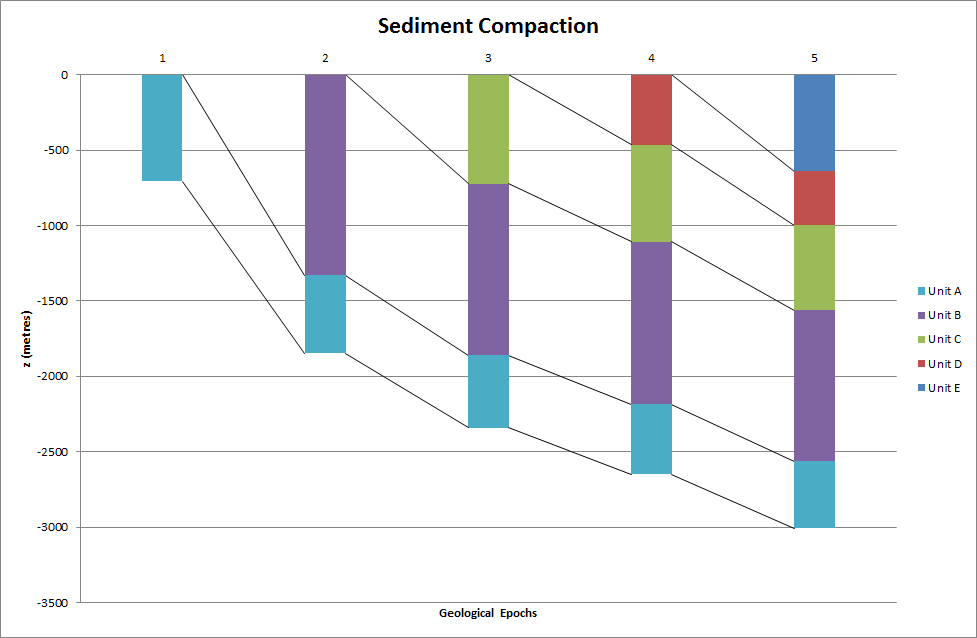
\includegraphics[width=0.9\linewidth]{fig-models/Compaction_of_Sediment.png}}
  \caption{
  Illustration of the compaction of geological layers (with different colors) through time. \label{decay:app:sediment:fig:layers}
  }
\end{figure}
%\clearpage % flush figures decay:app:sediment:fig:layers


When we drill a well at present time through the right-most column of
sediments in Figure~\ref{decay:app:sediment:fig:layers}, we can measure
the thickness of the sediment in (say) the bottom layer. Let $L_1$ be
this thickness.  Assuming that the volume of sediment remains constant
through time, we have that the initial volume, $\int_0^{L_{1,0}}
\phi_1 dz$, must equal the volume seen today,
$\int_{\ell-L_1}^{\ell}\phi_1 dz$, where $\ell$ is the depth of the
bottom of the sediment in the present day configuration.  After having
solved for $\phi_1$ as a function of $z$, we can then find the
original thickness $L_{1,0}$ of the sediment from the equation

\[ \int_0^{L_{1,0}} \phi_1 dz = \int_{\ell-L_1}^{\ell}\phi_1 dz \tp \]
In hydrocarbon exploration it is important to know $L_{1,0}$ and the
compaction history of the various layers of sediments.

\section{Vertical motion of a body in a viscous fluid}
\label{decay:app:drag}


A body moving vertically through a fluid (liquid or gas) is subject to
three different types of forces: the gravity force, \href{{http://en.wikipedia.org/wiki/Drag_(physics)}}{the drag force},
and the buoyancy force.

\subsection{Overview of forces}

Taking the upward direction as positive,
the gravity force is $F_g= -mg$, where $m$ is the mass of the body and
$g$ is the acceleration of gravity.
The uplift or buoyancy force (``Archimedes force'') is $F_b = \varrho gV$,
where $\varrho$ is the density of the fluid and
$V$ is the volume of the body.

The drag force is of two types, depending on the Reynolds number
\begin{equation}
\hbox{Re} = \frac{\varrho d|v|}{\mu},
\end{equation}
where $d$ is the diameter of the body in
the direction perpendicular to the flow, $v$ is the velocity of the
body, and $\mu$ is the dynamic viscosity of the fluid.
When $\hbox{Re} < 1$, the drag force is fairly well modeled by
the so-called Stokes' drag,
which for a spherical body of diameter $d$ reads
\begin{equation}
F_d^{(S)} = - 3\pi d\mu v
\tp
\end{equation}
Quantities are taken as positive in the upwards vertical direction, so
if $v>0$ and the body moves upwards, the drag force acts downwards and
become negative, in accordance with the minus sign in expression for
$F_d^{(S)}$.

For large Re, typically $\hbox{Re} > 10^3$, the drag force is quadratic
in the velocity:
\begin{equation}
F_d^{(q)} = -{1\over2}C_D\varrho A|v|v,
\end{equation}
where $C_D$ is a dimensionless drag coefficient depending on the body's shape,
and $A$ is the cross-sectional area as
produced by a cut plane, perpendicular to the motion, through the thickest
part of the body. The superscripts $\,{}^q$ and $\,{}^S$ in
$F_d^{(S)}$ and $F_d^{(q)}$ indicate Stokes drag and quadratic drag,
respectively.

\subsection{Equation of motion}

All the mentioned forces act in the vertical direction.
Newton's second law of motion applied to the body says that the sum of
these forces must equal the mass of the body times its acceleration
$a$ in the vertical direction.

\begin{equation*} ma = F_g + F_d^{(S)} + F_b \tp\end{equation*}
Here we have chosen to model the fluid resistance by the Stokes drag.
Inserting the expressions for the forces yields

\[  ma = -mg - 3\pi d\mu v + \varrho gV
\tp
\]
The unknowns here are $v$ and $a$, i.e., we have two unknowns but only
one equation. From kinematics in physics we know that
the acceleration is the time derivative of the velocity: $a = dv/dt$.
This is our second equation.
We can easily eliminate $a$ and get a single differential equation for $v$:

\[ m{dv\over dt} = -mg - 3\pi d\mu v + \varrho gV
\tp
\]
A small rewrite of this equation is handy: We express $m$ as $\varrho_bV$,
where $\varrho_b$ is the density of the body, and we divide by
the mass to get

\begin{equation}
v^{\prime}(t) = - \frac{3\pi d\mu}{\varrho_b V} v + g\left(\frac{\varrho}{\varrho_b} -1\right)
\label{decay:app:fallingbody:model:S}
\tp
\end{equation}
We may introduce the constants
\begin{equation}
a = \frac{3\pi d\mu}{\varrho_b V},\quad
b = g\left(\frac{\varrho}{\varrho_b} -1\right),
\end{equation}
so that the structure of the differential equation becomes obvious:

\begin{equation}
v^{\prime}(t) = -av(t) + b
\label{decay:app:fallingbody:gmodel:S}
\tp
\end{equation}
The corresponding initial condition is $v(0)=v_0$ for some prescribed
starting velocity $v_0$.

This derivation can be repeated with the quadratic drag force
$F_d^{(q)}$, leading to the result

\begin{equation}
v^{\prime}(t) =
-{1\over2}C_D{\varrho A\over\varrho_b V}|v|v +
g\left({\varrho\over\varrho_b} - 1\right)
\tp
\label{decay:app:fallingbody:model:q}
\end{equation}
Defining

\begin{equation}
a = {1\over2}C_D{\varrho A\over\varrho_b V},
\end{equation}
and $b$ as above, we can write (\ref{decay:app:fallingbody:model:q}) as
\begin{equation}
v^{\prime}(t) = -a|v|v + b
\tp
\label{decay:app:fallingbody:gmodel:q}
\end{equation}

\index{terminal velocity}

\subsection{Terminal velocity}

An interesting aspect of (\ref{decay:app:fallingbody:gmodel:S}) and
(\ref{decay:app:fallingbody:gmodel:q}) is whether $v$ will approach
a final constant value,
the so-called \emph{terminal velocity} $v_T$, as $t\rightarrow\infty$.
A constant $v$ means that
$v^{\prime}(t)\rightarrow 0$ as $t\rightarrow\infty$ and therefore
the terminal velocity $v_T$ solves

\[ 0 = -av_T + b \]
and
\[ 0 = -a|v_T|v_T + b\tp \]
The former equation implies $v_T = b/a$, while the latter has solutions
$v_T =-\sqrt{|b|/a}$ for a falling body ($v_T < 0$) and
$v_T = \sqrt{b/a}$ for a rising body ($v_T>0$).

\subsection{A Crank-Nicolson scheme}

Both governing equations, the Stokes' drag model
(\ref{decay:app:fallingbody:gmodel:S}) and the quadratic drag model
(\ref{decay:app:fallingbody:gmodel:q}), can be readily solved
by the Forward Euler scheme. For higher accuracy one can use
the Crank-Nicolson method, but a straightforward application
of this method gives
a nonlinear equation in the new unknown value $v^{n+1}$ when applied to
(\ref{decay:app:fallingbody:gmodel:q}):

\begin{equation}
\frac{v^{n+1}-v^n}{\Delta t}
= -a\half(|v^{n+1}|v^{n+1} + |v^n|v^n) + b
\label{decay:app:fallingbody:gmodel:CN}
\tp
\end{equation}
The first term on the right-hand side of (\ref{decay:app:fallingbody:gmodel:CN})
is the arithmetic average of $-|v|v$ evaluated at time levels $n$ and $n+1$.

Instead of approximating the term $-|v|v$ by an arithmetic
average, we can use a \emph{geometric mean}:

\index{geometric mean}
\index{averaging!geometric}

\begin{equation}
(|v|v)^{n+\half} \approx |v^n|v^{n+1}
\tp
\end{equation}
The error is of second order in $\Delta t$, just as for the arithmetic
average and the centered finite difference approximation in
(\ref{decay:app:fallingbody:gmodel:CN}). With the geometric mean,
the resulting discrete equation

\[
\frac{v^{n+1}-v^n}{\Delta t} = - a|v^{n}|v^{n+1} + b
\]
becomes a \emph{linear} equation in $v^{n+1}$, and we can
therefore easily solve for $v^{n+1}$:

\begin{equation}
v^{n+1} = \frac{v_n + \Delta t b^{n+\half}}{1 + \Delta t a^{n+\half}|v^{n}|}\tp
\label{decay:app:fallingbody:gmodel:q:CN}
\end{equation}

Using a geometric mean instead of an arithmetic mean in the Crank-Nicolson
scheme is an attractive method for avoiding a nonlinear algebraic
equation when discretizing a nonlinear ODE.

% Is the error actually of second order for an arbitrary a(u)u term?

\subsection{Physical data}

Suitable values of $\mu$ are $1.8\cdot 10^{-5}\hbox{ Pa}\, \hbox{s}$ for air
and $8.9\cdot 10^{-4}\hbox{ Pa}\, \hbox{s}$ for water.
Densities can be taken as $1.2\hbox{ kg/m}^3$ for air and as
$1.0\cdot 10^3\hbox{ kg/m}^3$ for water. For considerable vertical
displacement in the atmosphere one should take into account that
the density of air varies with the altitude, see Section~\ref{decay:app:atm}.
One possible density variation arises from the one-layer model
in the mentioned section.

Any density variation makes $b$ time dependent and we need
$b^{n+\half}$ in (\ref{decay:app:fallingbody:gmodel:q:CN}).
To compute the density that enters
$b^{n+\half}$ we must also compute the vertical
position $z(t)$ of the body. Since $v=dz/dt$, we can use a centered
difference approximation:

\[ \frac{z^{n+\half} - z^{n-\half}}{\Delta t} = v^n
\quad\Rightarrow\quad z^{n+\half} = z^{n-\half}+\Delta t\, v^n\tp\]
This $z^{n+\half}$ is used in the expression for $b$
to compute $\varrho(z^{n+\half})$ and then $b^{n+\half}$.

The \href{{http://en.wikipedia.org/wiki/Drag_coefficient}}{drag coefficient} $C_D$ depends heavily
on the shape of the body.  Some values are: 0.45 for a sphere, 0.42
for a semi-sphere, 1.05 for a cube, 0.82 for a long cylinder (when the
center axis is in the vertical direction), 0.75 for a rocket,
1.0-1.3 for a man in upright position, 1.3 for a flat plate perpendicular
to the flow, and
0.04 for a streamlined, droplet-like body.

\subsection{Verification}

To verify the program, one may assume a heavy body in air such that the $F_b$
force can be neglected, and further assume a small velocity such that the
air resistance $F_d$ can also be neglected. This can be obtained by
setting $\mu$ and $\varrho$ to zero. The motion then leads to
the velocity
$v(t)=v_0 - gt$, which is linear in $t$ and therefore should be
reproduced to machine precision (say tolerance $10^{-15}$) by any
implementation based on the Crank-Nicolson or Forward Euler schemes.

Another verification, but not as powerful as the one above,
can be based on computing the terminal velocity and comparing with
the exact expressions.
The advantage of this verification is that we can also
test the situation $\varrho\neq 0$.

As always, the method of manufactured solutions can be applied to
test the implementation of all terms in the governing equation, but
then the solution has no physical relevance in general.

\index{scaling}

\subsection{Scaling}
\label{decay:app:drag:scaling}

Applying scaling, as described in Section~\ref{decay:app:scaling},
will for the linear case reduce the need to estimate values for
seven parameters down to choosing one value of a single dimensionless parameter

\[ \beta = \frac{\varrho_b gV\left(\frac{\varrho}{\varrho_b} -1\right)}{3\pi d\mu I},\]
provided $I\neq 0$. If the motion starts from rest, $I=0$, the scaled
problem reads

\[ \bar u^{\prime}=1-\bar u, \quad \bar u(0)=0,\]
and there is
no need for estimating physical parameters (!).
This means that there is a single universal solution to the problem
of a falling body starting from rest:
$\bar u(t) = 1 - e^{-\bar t}$. All real
physical cases correspond to stretching the $\bar t$ axis and the $\bar u$
axis in this dimensionless solution. More precisely, the physical velocity
$u(t)$ is related to the dimensionless velocity $\bar u(\bar t)$ through

\[ u = \frac{\varrho_bgV\left(\frac{\varrho}{\varrho_b} -1\right)}{3\pi d\mu}\bar u(t/(g(\varrho/\varrho_b -1))) =
\frac{\varrho_bgV\left(\frac{\varrho}{\varrho_b} -1\right)}{3\pi d\mu}(1 -
e^{t/(g(\varrho/\varrho_b -1))})\tp\]

\section{Viscoelastic materials}
\label{decay:app:viscoelasticity}

\index{Kelvin-Voigt material model}
\index{viscoelasticity}

When stretching a rod made of a perfectly elastic material, the
elongation (change in the rod's
length) is proportional to the magnitude of the applied force.
Mathematical models for material behavior under application of
external forces use \emph{strain} $\varepsilon$
and \emph{stress} $\sigma$ instead of elongation and
forces. Strain is relative change in elongation and stress is force
per unit area. An elastic material has a linear relation between
stress and strain:  $\sigma = E\varepsilon$. This is a good model
for many materials, but frequently the velocity of the deformation
(or more precisely, the strain rate $\varepsilon^{\prime}$)
also influences the stress. This is particularly the case for
materials like organic polymers, rubber, and wood. When the stress
depends on both the strain and the strain rate, the material is
said to be viscoelastic. A common model relating forces to deformation
is the \href{{https://en.wikipedia.org/wiki/Kelvin-Voigt_material}}{Kelvin-Voigt model}:

\begin{equation}
\sigma(t) = E\varepsilon(t) + \eta\varepsilon^{\prime}(t)\tp
\label{decay:app:viscoelasticity:se}
\end{equation}
Compared to a perfectly elastic material, which deforms instantaneously
when a force is acting, a Kelvin-Voigt material will spend some time
to elongate. For example, when an elastic rod is subject to a constant
force $\stress$ at $t=0$, the strain immediately adjusts to $\varepsilon
=\sigma/E$. A Kelvin-Voigt material, however, has a response
$\varepsilon(t) = \frac{\sigma}{E}(1-e^{Et/\eta})$. Removing the force
when the strain is $\varepsilon(t_1) = I$ will for an elastic material
immediately bring the strain back to zero, while a Kelvin-Voigt
material will decay: $\varepsilon = Ie^{-(t-t_1)E/\eta)}$.

Introducing $u$ for $\varepsilon$ and treating $\stress(t)$ as a
given function, we can write the Kelvin-Voigt model in our standard form

\begin{equation}
u^{\prime}(t) = -au(t) + b(t),
\end{equation}
with $a = E/\eta$ and $b(t)=\stress(t)/\eta$. An initial condition,
usually $u(0)=0$, is needed.




\section{Decay ODEs from solving a PDE by Fourier expansions}
\label{decay:app:diffusion:Fourier}

% Maybe move to diffusion part? Makes sense there too, or refer...or
% repeat, or make one exer with two k's and then generalize in diffusion

Suppose we have a partial differential equation
\[ \frac{\partial u}{\partial t} = \alpha\frac{\partial^2u}{\partial x^2}
+ f(x,t),
\]
with boundary conditions $u(0,t)=u(L,t)=0$ and initial condition
$u(x,0)=I(x)$. One may express the solution as
\[ u(x,t) = \sum_{k=1}^m A_k(t)e^{ikx\pi/L},\]
for appropriate unknown functions $A_k$, $k=1,\ldots,m$.
We use the complex exponential $e^{ikx\pi/L}$ for easy algebra, but
the physical $u$ is taken as the real part of any complex expression.
Note that the expansion in terms of $e^{ikx\pi/L}$ is compatible with
the boundary conditions: all functions $e^{ikx\pi/L}$ vanish for
$x=0$ and $x=L$. Suppose we can express $I(x)$ as

\[ I(x) = \sum_{k=1}^m I_ke^{ikx\pi/L}
\tp
\]
Such an expansion can be computed by well-known Fourier expansion techniques,
but those details are not important here.
Also, suppose we can express the given $f(x,t)$ as
\[ f(x,t) = \sum_{k=1}^m b_k(t)e^{ikx\pi/L}
\tp
\]
Inserting the expansions for $u$
and $f$ in the differential equations demands that all terms corresponding
to a given $k$ must be equal. The calculations result in the follow
system of ODEs:

\[
A_k^{\prime}(t) = -\alpha\frac{k^2\pi^2}{L^2} + b_k(t),\quad k=1,\ldots,m
\tp
\]
From the initial condition
\[ u(x,0)=\sum_k A_k(0)e^{ikx\pi/L}=I(x)=\sum_k I_k e^{(ikx\pi/L)},\]
so it follows that $A_k(0)=I_k$, $k=1,\ldots,m$. We then have $m$
equations of the form $A_k^{\prime}=-a A_k +b$, $A_k(0)=I_k$, for
appropriate definitions of $a$ and $b$. These ODE problems
are independent of each other such that we can solve one problem
at a time. The outlined technique is a quite common solution approach to
partial differential equations.

\paragraph{Remark.}
Since $a_k$ depends on $k$ and the stability of the
Forward Euler scheme demands $a_k\Delta t \leq 1$, we get that $\Delta
t \leq \alpha^{-1}L^2\pi^{-2} k^{-2}$ for this scheme.  Usually, quite
large $k$ values are needed to accurately represent the given
functions $I$ and $f$ so that $\Delta t$ in the Forward Euler scheme
needs to be very small for these large values of $k$.  Therefore, the
Crank-Nicolson and Backward Euler schemes, which allow larger $\Delta
t$ without any growth in the solutions, are more popular choices when
creating time-stepping algorithms for partial differential equations
of the type considered in this example.


\section{Exercises}



% --- begin exercise ---
\begin{doconceexercise}
\refstepcounter{doconceexercisecounter}

\subsection*{Problem \thedoconceexercisecounter: Radioactive decay of Carbon-14}
\addcontentsline{loe}{doconceexercise}{Problem \thedoconceexercisecounter: Radioactive decay of Carbon-14}

\label{decay:app:exer:radio:C14}

The \href{{http://en.wikipedia.org/wiki/Carbon-14}}{Carbon-14} isotope,
whose radioactive decay is used extensively in dating organic material
that is tens of thousands of years old, has a half-life of $5,730$
years.  Determine the age of an organic material that contains 8.4 percent
of its initial amount of Carbon-14.  Use a time unit of 1 year in the
computations.  The uncertainty in the half time of Carbon-14 is $\pm
40$ years.  What is the corresponding uncertainty in the estimate of
the age?

% --- begin hint in exercise ---

\paragraph{Hint 1.}
Let $A$ be the amount of Carbon-14. The ODE problem is then
$A^{\prime}(t)=-aA(t)$, $A(0)=I$. Introduced the scaled amount
$u=A/I$. The ODE problem for $u$ is $u^{\prime}=-au$, $u(0)=1$.
Measure time in years.
Simulate until the first mesh point $t_m$ such that $u(t_m)\leq 0.084$.

% --- end hint in exercise ---

% --- begin hint in exercise ---

\paragraph{Hint 2.}
Use simulations with $5,730\pm 40$ y as input
and find the corresponding uncertainty interval for the result.

% --- end hint in exercise ---


% removed !bsol ... !esol environment (because of the command-line option --without_solutions)
\noindent Filename: \texttt{carbon14}.

\end{doconceexercise}
% --- end exercise ---




% --- begin exercise ---
\begin{doconceexercise}
\refstepcounter{doconceexercisecounter}

\subsection*{Exercise \thedoconceexercisecounter: Derive schemes for Newton's law of cooling}
\addcontentsline{loe}{doconceexercise}{Exercise \thedoconceexercisecounter: Derive schemes for Newton's law of cooling}

\label{decay:app:exer:cooling:schemes}

Show in detail how we can apply the ideas of the Forward Euler,
Backward Euler, and Crank-Nicolson
discretizations to derive explicit
computational formulas for new temperature values in Newton's law of
cooling (see Section~\ref{decay:app:Newton:cooling}):

\[
\frac{dT}{dt} = -k(T-T_s(t)),\quad T(0)=T_0\tp
\]
Here, $T$ is the temperature of the body, $T_s(t)$ is the temperature
of the surroundings, $t$ is time, $k$ is the heat transfer
coefficient, and $T_0$ is the initial temperature of the body.
Summarize the discretizations in a $\theta$-rule
such that you can get the three
schemes from a single formula by varying the $\theta$ parameter.


% removed !bsol ... !esol environment (because of the command-line option --without_solutions)
\noindent Filename: \Verb!schemes_cooling!.

\end{doconceexercise}
% --- end exercise ---




% --- begin exercise ---
\begin{doconceexercise}
\refstepcounter{doconceexercisecounter}

\subsection*{Exercise \thedoconceexercisecounter: Implement schemes for Newton's law of cooling}
\addcontentsline{loe}{doconceexercise}{Exercise \thedoconceexercisecounter: Implement schemes for Newton's law of cooling}

\label{decay:app:exer:cooling:py}

The goal of this exercise is to implement the schemes from
Exercise~\ref{decay:app:exer:cooling:schemes} and investigate
several approaches for verifying the implementation.


\subex{a)}
Implement the $\theta$-rule from
Exercise~\ref{decay:app:exer:cooling:schemes} in a function

\begin{cod}{cbg_blue1}\begin{Verbatim}[numbers=none,fontsize=\fontsize{9pt}{9pt},baselinestretch=0.95,xleftmargin=2mm]
cooling(T0, k, T_s, t_end, dt, theta=0.5)
\end{Verbatim}
\end{cod}
\noindent
where \texttt{T0} is the initial temperature, \texttt{k} is
the heat transfer coefficient, \Verb!T_s! is a function of \texttt{t} for
the temperature of the
surroundings, \Verb!t_end! is the end time of the simulation, \texttt{dt} is the
time step, and \texttt{theta} corresponds to $\theta$.  The \texttt{cooling}
function should return the temperature as an array \texttt{T} of values at
the mesh points and the time mesh \texttt{t}.


% removed !bsol ... !esol environment (because of the command-line option --without_solutions)

\subex{b)}
In the case $\lim_{t\rightarrow\infty}T_s(t)=C=\mbox{const}$,
explain why $T(t)\rightarrow C$. Construct an example where you
can illustrate this property in a plot. Implement a corresponding
test function that checks the correctness of the asymptotic
value of the solution.


% removed !bsol ... !esol environment (because of the command-line option --without_solutions)

\subex{c)}
A piecewise constant surrounding temperature,

\[ T_s(t) = \left\lbrace\begin{array}{ll} C_0,& 0\leq t\leq t^*\\ 
C_1, & t>t^*,\end{array}\right.
\]
corresponds to a sudden change in the environment
at $t=t^*$. Choose $C_0=2T_0$, $C_1=\frac{1}{2}T_0$, and
$t^*=3/k$. Plot the solution $T(t)$ and explain why it seems physically
reasonable.


% removed !bsol ... !esol environment (because of the command-line option --without_solutions)

\subex{d)}
We know from the ODE $u^\prime =-au$ that the Crank-Nicolson scheme
can give non-physical oscillations for $\Delta t > 2/a$.
In the present problem, this results indicates
that the Crank-Nicolson scheme give undesired
oscillations for $\Delta t > 2/k$.
Discuss if this a potential problem in the physical case from c).


% removed !bsol ... !esol environment (because of the command-line option --without_solutions)

\subex{e)}
Find an expression for the exact solution of
$T^{\prime} = -k(T-T_s(t))$, $T(0)=T_0$.
Construct a test case and compare the
numerical and exact solution in a plot.

Find a value of the time step
$\Delta t$ such that the two solution curves cannot (visually) be
distinguished from each other. Many scientists will claim that such a
plot provides evidence for a correct implementation, but point out why
there still may be errors in the code.  Can you introduce bugs in the
\texttt{cooling} function and still achieve visually coinciding curves?

% --- begin hint in exercise ---

\paragraph{Hint.}
The exact solution can be derived by multiplying (\ref{decay:Newton:cooling})
by the integrating factor $e^{kt}$.

% --- end hint in exercise ---


% removed !bsol ... !esol environment (because of the command-line option --without_solutions)

\subex{f)}
Implement a test function for checking that the solution returned by
the \texttt{cooling} function is identical to the exact numerical
solution of the problem (to machine precision) when $T_s$ is constant.

% --- begin hint in exercise ---

\paragraph{Hint.}
The exact solution of the
discrete equations in the case $T_s$ is a constant can be found by
introducing $u=T-T_s$ to get a problem $u^{\prime}=-ku$, $u(0)=T_0-T_s$.
The solution of the discrete equations is then of the form
$u^{n}=(T_0-T_s)A^n$ for some amplification factor $A$. The
expression for $T^n$ is then $T^n = T_s(t_n) + u^n =
T_s + (T_0-T_s)A^n$.
We find that

\[ A = \frac{1 - (1-\theta) k\Delta t}{1 + \theta k\Delta t}\tp\]
The test function, testing several $\theta$ values for a quite coarse
mesh, may take the form

\begin{cod}{cbg_blue1}\begin{Verbatim}[numbers=none,fontsize=\fontsize{9pt}{9pt},baselinestretch=0.95,xleftmargin=2mm]
def test_discrete_solution():
    """
    Compare the numerical solution with an exact solution of the scheme
    when the T_s is constant.
    """
    T_s = 10
    T0 = 2
    k = 1.2
    dt = 0.1   # can use any mesh
    N_t = 6    # any no of steps will do
    t_end = dt*N_t
    t = np.linspace(0, t_end, N_t+1)

    for theta in [0, 0.5, 1, 0.2]:
        u, t = cooling(T0, k, lambda t: T_s , t_end, dt, theta)
        A = (1 - (1-theta)*k*dt)/(1 + theta*k*dt)
        u_discrete_exact = T_s + (T0-T_s)*A**(np.arange(len(t)))
        diff = np.abs(u - u_discrete_exact).max()
        print 'diff computed and exact discrete solution:', diff
        tol = 1E-14
        success = diff < tol
        assert success, 'diff=%g' % diff
\end{Verbatim}
\end{cod}
\noindent
Running this function shows that the \texttt{diff} variable is \texttt{3.55E-15}
as maximum so a tolerance of $10^{-14}$ is appropriate.
This is a good test that the \texttt{cooling} function works!

% --- end hint in exercise ---

\noindent Filename: \texttt{cooling}.

\end{doconceexercise}
% --- end exercise ---




% --- begin exercise ---
\begin{doconceexercise}
\refstepcounter{doconceexercisecounter}

\subsection*{Exercise \thedoconceexercisecounter: Find time of murder from body temperature}
\addcontentsline{loe}{doconceexercise}{Exercise \thedoconceexercisecounter: Find time of murder from body temperature}

\label{decay:app:exer:cooling:murder}

% \href{{http://www.biology.arizona.edu/BioMath/tutorials/Applications/Cooling.html}}{\nolinkurl{http://www.biology.arizona.edu/BioMath/tutorials/Applications/Cooling.html}}

A detective measures the temperature of a dead body to be 26.7 C at 2
pm. One hour later the temperature is 25.8 C. The question is when
death occurred.

Assume that Newton's law of cooling (\ref{decay:Newton:cooling}) is an
appropriate mathematical model for the evolution of the temperature in
the body.  First, determine $k$ in (\ref{decay:Newton:cooling}) by
formulating a Forward Euler approximation with one time steep from
time 2 am to time 3 am, where knowing the two temperatures allows for
finding $k$. Assume the temperature in the air to be 20 C. Thereafter,
simulate the temperature evolution from the time of murder, taken as
$t=0$, when $T=37\hbox{ C}$, until the temperature reaches 25.8 C. The
corresponding time allows for answering when death occurred.


% removed !bsol ... !esol environment (because of the command-line option --without_solutions)
\noindent Filename: \texttt{detective}.

\end{doconceexercise}
% --- end exercise ---




% --- begin exercise ---
\begin{doconceexercise}
\refstepcounter{doconceexercisecounter}

\subsection*{Exercise \thedoconceexercisecounter: Simulate an oscillating cooling process}
\addcontentsline{loe}{doconceexercise}{Exercise \thedoconceexercisecounter: Simulate an oscillating cooling process}

\label{decay:app:exer:cooling:osc}

The surrounding temperature $T_s$ in Newton's law of cooling
(\ref{decay:Newton:cooling}) may vary in time. Assume that the
variations are periodic with period $P$ and amplitude $a$ around
a constant mean temperature $T_m$:

\begin{equation}
T_s(t) = T_m + a\sin\left(\frac{2\pi}{P}t\right)
\tp
\end{equation}
Simulate a process with the following data: $k=0.05 \hbox{ min}^{-1}$,
$T(0)=5$ C, $T_m=25$ C, $a=2.5$ C, and $P=1$ h, $P=10$ min, and $P=6$ h.
Plot the $T$ solutions and $T_s$ in the same plot.


% removed !bsol ... !esol environment (because of the command-line option --without_solutions)
\noindent Filename: \Verb!osc_cooling!.

\end{doconceexercise}
% --- end exercise ---




% --- begin exercise ---
\begin{doconceexercise}
\refstepcounter{doconceexercisecounter}

\subsection*{Exercise \thedoconceexercisecounter: Simulate stochastic radioactive decay}
\addcontentsline{loe}{doconceexercise}{Exercise \thedoconceexercisecounter: Simulate stochastic radioactive decay}

\label{decay:app:exer:stoch:nuclear}

The purpose of this exercise is to implement the stochastic model
described in Section~\ref{decay:app:nuclear} and show that its
mean behavior approximates the solution of the corresponding
ODE model.

The simulation goes on for a time interval $[0,T]$ divided into
$N_t$ intervals of length $\Delta t$. We start with $N_0$
atoms. In some time interval, we have $N$ atoms that have survived.
Simulate $N$ Bernoulli trials with probability $\lambda\Delta t$
in this interval by drawing $N$ random numbers, each being 0 (survival)
or 1 (decay), where the probability of getting 1 is $\lambda\Delta t$.
We are interested in the number of decays, $d$, and the number of
survived atoms in the next interval is then $N-d$.
The Bernoulli trials
are simulated by drawing $N$ uniformly distributed real numbers on
$[0,1]$ and saying that 1 corresponds to a value less than $\lambda\Delta t$:

\begin{cod}{cbg_blue1}\begin{Verbatim}[numbers=none,fontsize=\fontsize{9pt}{9pt},baselinestretch=0.95,xleftmargin=2mm]
# Given lambda_, dt, N
import numpy as np
uniform = np.random.uniform(N)
Bernoulli_trials = np.asarray(uniform < lambda_*dt, dtype=np.int)
d = Bernoulli_trials.size
\end{Verbatim}
\end{cod}
\noindent
Observe that \Verb!uniform < lambda_*dt! is a boolean array whose true
and false values become 1 and 0, respectively, when converted to an
integer array.

Repeat the simulation over $[0,T]$ a large number of times, compute the average
value of $N$ in each interval, and compare with the solution of
the corresponding ODE model.
\noindent Filename: \Verb!stochastic_decay!.

\end{doconceexercise}
% --- end exercise ---




% --- begin exercise ---
\begin{doconceexercise}
\refstepcounter{doconceexercisecounter}

\subsection*{Problem \thedoconceexercisecounter: Radioactive decay of two substances}
\addcontentsline{loe}{doconceexercise}{Problem \thedoconceexercisecounter: Radioactive decay of two substances}

\label{decay:app:exer:radio:twosubst}

Consider two radioactive substances A and B. The nuclei in substance A
decay to form nuclei of type B with a half-life $A_{1/2}$, while
substance B decay to form type A nuclei with a half-life $B_{1/2}$.
Letting $u_A$ and $u_B$ be the fractions of the initial amount of
material in substance A and B, respectively, the following system of
ODEs governs the evolution of $u_A(t)$ and $u_B(t)$:
\begin{align}
\frac{1}{\ln 2} u_A^{\prime} &= u_B/B_{1/2} - u_A/A_{1/2},\\ 
\frac{1}{\ln 2} u_B^{\prime} &= u_A/A_{1/2} - u_B/B_{1/2},
\end{align}
with $u_A(0)=u_B(0)=1$.


\subex{a)}
Make a simulation program that solves for $u_A(t)$ and $u_B(t)$.

\subex{b)}
Verify the implementation by computing analytically
the limiting values of
$u_A$ and $u_B$ as $t\rightarrow \infty$ (assume $u_A^{\prime},u_B^{\prime}\rightarrow 0$)
and comparing these with those obtained numerically.

\subex{c)}
Run the program for the case of $A_{1/2}=10$ minutes and $B_{1/2}=50$ minutes.
Use a time unit of 1 minute. Plot $u_A$ and $u_B$ versus time in the same
plot.

\noindent Filename: \Verb!radioactive_decay_2subst!.

\end{doconceexercise}
% --- end exercise ---




% --- begin exercise ---
\begin{doconceexercise}
\refstepcounter{doconceexercisecounter}

\subsection*{Exercise \thedoconceexercisecounter: Simulate a simple chemical reaction}
\addcontentsline{loe}{doconceexercise}{Exercise \thedoconceexercisecounter: Simulate a simple chemical reaction}

\label{decay:app:exer:kinetics:AB}

Consider the simple chemical reaction where a substance A is turned
into a substance B according to

\begin{align*}
\frac{d[A]}{dt} &= -k[A],\\ 
\frac{d[B]}{dt} &= k[A],\\ 
\end{align*}
where $[A]$ and $[B]$ are the concentrations of A and B, respectively.
It may be a challenge to find appropriate values of $k$, but we can avoid
this problem by working with a scaled model (as explained in
Section~\ref{decay:app:scaling}).
Scale the model above, using a time scale $1/k$, and use
the initial concentration
of $[A]$ as scale for $[A]$ and $[B]$. Show that the scaled system
reads

\begin{align*}
\frac{du}{dt} &= -u,\\ 
\frac{dv}{dt} &= u,\\ 
\end{align*}
with initial conditions $u(0)=1$, and $v(0)=\alpha$, where
$\alpha = [B](0)/[A](0)$ is a dimensionless number, and
$u$ and $v$ are the scaled concentrations of $[A]$ and $[B]$,
respectively. Implement a numerical scheme that can be used to
find the solutions
$u(t)$ and $v(t)$. Visualize $u$ and $v$ in the same plot.
\noindent Filename: \Verb!chemcial_kinetics_AB!.

\end{doconceexercise}
% --- end exercise ---




% --- begin exercise ---
\begin{doconceexercise}
\refstepcounter{doconceexercisecounter}

\subsection*{Exercise \thedoconceexercisecounter: Simulate an $n$-th order chemical reaction}
\addcontentsline{loe}{doconceexercise}{Exercise \thedoconceexercisecounter: Simulate an $n$-th order chemical reaction}

\label{decay:app:exer:kinetics:ABn}

An $n$-order chemical reaction, generalizing the model in
Exercise~\ref{decay:app:exer:kinetics:AB}, takes the form

\begin{align*}
\frac{d[A]}{dt} &= -k[A]^n,\\ 
\frac{d[B]}{dt} &= k[A]^n,\\ 
\end{align*}
where symbols are as defined in Exercise~\ref{decay:app:exer:kinetics:AB}.
Bring this model on dimensionless form, using a time scale $[A](0)^{n-1}/k$,
and show that the dimensionless model simplifies to

\begin{align*}
\frac{du}{dt} &= -u^n,\\ 
\frac{dv}{dt} &= u^n,\\ 
\end{align*}
with $u(0)=1$ and $v(0)=\alpha = [B](0)/[A](0)$. Solve numerically for
$u(t)$ and show a plot with $u$ for $n=0.5, 1, 2, 4$.
\noindent Filename: \Verb!chemcial_kinetics_ABn!.

\end{doconceexercise}
% --- end exercise ---




% --- begin exercise ---
\begin{doconceexercise}
\refstepcounter{doconceexercisecounter}

\subsection*{Exercise \thedoconceexercisecounter: Simulate a biochemical process}
\addcontentsline{loe}{doconceexercise}{Exercise \thedoconceexercisecounter: Simulate a biochemical process}

\label{decay:app:exer:MMK}

The purpose of this exercise is to simulate the ODE system
(\ref{decay:app:MMK:ES1})-(\ref{decay:app:MMK:E1}) modeling a simple
biochemical process.


\subex{a)}
Scale (\ref{decay:app:MMK:ES1})-(\ref{decay:app:MMK:E1}) such that
we can work with dimensionless parameters, which are easier to prescribe.
Introduce

\[ \bar Q = \frac{[ES]}{Q_c},\quad
\bar P = \frac{P}{P_c},\quad \bar S = \frac{S}{S_0},\quad \bar E = \frac{E}{E_0},\quad \bar t = \frac{t}{t_c},\]
where appropriate scales are

\[ Q_c = \frac{S_0E_0}{K},\quad P_c = Q_c, \quad t_c=\frac{1}{k_+E_0},\]
with $K=(k_v+k_-)/k_+$ (Michaelis constant). Show that the scaled
system becomes

\begin{align}
\frac{d\bar Q}{d\bar t} &= \alpha (\bar E\bar S
- \bar Q),
\label{decay:app:MMK:Q2}\\ 
\frac{d\bar P}{d\bar t} &= \beta\bar Q,
\label{decay:app:MMK:P2}\\ 
\frac{d\bar S}{d\bar t} &= -\bar E\bar S
+ (1 - \beta\alpha^{-1})\bar Q,
\label{decay:app:MMK:S2}\\ 
\epsilon\frac{d\bar E}{d\bar t} &= -\bar E\bar S + \bar Q,
\label{decay:app:MMK:E2}
\end{align}
where we have three dimensionless parameters

\[ \alpha = \frac{K}{E_0},\quad \beta = \frac{k_v}{k_+ E_0},\quad
\epsilon = \frac{E_0}{S_0}\tp
\]
The corresponding initial conditions are $\bar Q=\bar P=0$ and
$\bar S=\bar E=1$.


% removed !bsol ... !esol environment (because of the command-line option --without_solutions)

\subex{b)}
Implement a function for
solving (\ref{decay:app:MMK:Q2})-(\ref{decay:app:MMK:E2}).


% removed !bsol ... !esol environment (because of the command-line option --without_solutions)

\subex{c)}
There are two conservation equations implied by
(\ref{decay:app:MMK:ES1})-(\ref{decay:app:MMK:E1}):

\begin{align}
[ES] + [E] &= E_0,\\ 
[ES] + [S] + [P] &= S_0\tp
\end{align}
Derive these two equations. Use these properties in the function
in b) to do a partial verification of the solution at each time step.


% removed !bsol ... !esol environment (because of the command-line option --without_solutions)

\subex{d)}
Simulate a case with $T=8$, $\alpha = 1$, $\beta=4$, and two
$\epsilon$ values: 0.9 and 0.1.


% removed !bsol ... !esol environment (because of the command-line option --without_solutions)

\noindent Filename: \texttt{biochem}.

\end{doconceexercise}
% --- end exercise ---




% --- begin exercise ---
\begin{doconceexercise}
\refstepcounter{doconceexercisecounter}

\subsection*{Exercise \thedoconceexercisecounter: Simulate spreading of a disease}
\addcontentsline{loe}{doconceexercise}{Exercise \thedoconceexercisecounter: Simulate spreading of a disease}

\label{decay:app:exer:SIR}

The SIR model (\ref{decay:app:SIR:S})-(\ref{decay:app:SIR:R}) can be used
to simulate spreading of an epidemic disease.


\subex{a)}
Estimating the parameter $\beta$
is difficult so it can be handy to scale the equations. Use
$t_c=1/\nu$ as time scale, and scale $S$, $I$, and $R$ by
the population size $N=S(0)+I(0)+R(0)$. Show that the resulting dimensionless
model becomes

\begin{align}
\frac{d\bar S}{d\bar t} &= - R_0\bar S\bar I,
\label{decay:app:SIR:S2}\\ 
\frac{d\bar I}{d\bar t} &= R_0 \bar S\bar I - \bar I,
\label{decay:app:SIR:I2}\\ 
\frac{d\bar R}{d\bar t} &= I,
\label{decay:SIR:R2}\\ 
\bar S(0) &= 1-\alpha,\\ 
\bar I(0) &= \alpha,\\ 
\bar R(0) &= 0,
\end{align}
where $R_0$ and $\alpha$ are the only parameters in the problem:

\[ R_0 = \frac{N\beta}{\nu}, \quad \alpha = \frac{I(0)}{N}\tp\]
A quantity with a bar denotes a dimensionless version of that quantity, e.g,
$\bar t$ is dimensionless time, and $\bar t = \nu t$.


% removed !bsol ... !esol environment (because of the command-line option --without_solutions)

\subex{b)}
Show that the $R_0$ parameter governs whether the disease will spread
or not at $t=0$.

% --- begin hint in exercise ---

\paragraph{Hint.}
Spreading means $dI/dt>0$.

% --- end hint in exercise ---


% removed !bsol ... !esol environment (because of the command-line option --without_solutions)

\subex{c)}
Implement the scaled SIR model. Check at every time step,
as a verification, that
$\bar S + \bar I + \bar R = 1$.


% removed !bsol ... !esol environment (because of the command-line option --without_solutions)

\subex{d)}
Simulate the spreading of a disease where $R_0=2, 5$ and 2 percent of
the population is infected at time $t=0$.


% removed !bsol ... !esol environment (because of the command-line option --without_solutions)


\noindent Filename: \texttt{SIR}.

\end{doconceexercise}
% --- end exercise ---




% --- begin exercise ---
\begin{doconceexercise}
\refstepcounter{doconceexercisecounter}

\subsection*{Exercise \thedoconceexercisecounter: Simulate predator-prey interaction}
\addcontentsline{loe}{doconceexercise}{Exercise \thedoconceexercisecounter: Simulate predator-prey interaction}

\label{decay:app:exer:predprey}

Section~\ref{decay:app:predprey} describes a model for the
interaction of predator and prey populations, such as lynx and hares.


\subex{a)}
Scale the equations (\ref{decay:app:predprey:eqH})-(\ref{decay:app:predprey:eqL}).
Use the initial population $H(0)=H_0$ of $H$ has scale for $H$ and $L$, and
let the time scale be $1/(bH_0)$.


% removed !bsol ... !esol environment (because of the command-line option --without_solutions)

\subex{b)}
Implement the scaled model from a). Run illustrating cases how the
two populations develop.


% removed !bsol ... !esol environment (because of the command-line option --without_solutions)

\subex{c)}
The scaling in a) used a scale for $H$ and $L$ based on the
initial condition $H(0)=H_0$. An alternative scaling is to make
the ODEs as simple as possible by introducing separate scales
$H_c$ and $L_c$ for $H$ and $L$, respectively. Fit $H_c$,
$L_c$, and the time scale $t_c$ such that there are as few
dimensionless parameters as possible in the ODEs. Scale the initial
conditions. Compare the number and type of dimensionless parameters
with a).


% removed !bsol ... !esol environment (because of the command-line option --without_solutions)

\subex{d)}
Compute with the scaled model from c) and create plots to illustrate
the typical solutions.


% removed !bsol ... !esol environment (because of the command-line option --without_solutions)

\noindent Filename: \Verb!predator_prey!.

\end{doconceexercise}
% --- end exercise ---




% --- begin exercise ---
\begin{doconceexercise}
\refstepcounter{doconceexercisecounter}

\subsection*{Exercise \thedoconceexercisecounter: Simulate the pressure drop in the atmosphere}
\addcontentsline{loe}{doconceexercise}{Exercise \thedoconceexercisecounter: Simulate the pressure drop in the atmosphere}

\label{decay:app:exer:atm1}

We consider the models for atmospheric pressure in
Section~\ref{decay:app:atm}.
Make a program with three functions,

\begin{itemize}
 \item one computing the pressure $p(z)$ using a seven-layer model
   and varying $L$,

 \item one computing $p(z)$ using a seven-layer model,
   but with constant temperature in each layer, and

 \item one computing $p(z)$ based on the
   one-layer model.
\end{itemize}

\noindent
How can these implementations be verified? Should ease of verification
impact how you code the functions?
Compare the three models in a plot.
\noindent Filename: \Verb!atmospheric_pressure!.

\end{doconceexercise}
% --- end exercise ---




% --- begin exercise ---
\begin{doconceexercise}
\refstepcounter{doconceexercisecounter}

\subsection*{Exercise \thedoconceexercisecounter: Make a program for vertical motion in a fluid}
\addcontentsline{loe}{doconceexercise}{Exercise \thedoconceexercisecounter: Make a program for vertical motion in a fluid}

\label{decay:app:exer:drag:prog}

Implement the Stokes' drag model (\ref{decay:app:fallingbody:model:S})
and the quadratic drag model (\ref{decay:app:fallingbody:model:q}) from
Section~\ref{decay:app:drag}, using the Crank-Nicolson
scheme and a geometric mean for $|v|v$ as explained, and assume
constant fluid density.
At each time level, compute the Reynolds number
Re and choose the Stokes' drag model if $\hbox{Re} < 1$ and the
quadratic drag model otherwise.

The computation of the numerical solution should take place either in
a stand-alone function or in a solver class that looks up a problem
class for physical data. Create a module and equip it with pytest/nose
compatible test functions for automatically verifying the code.

Verification tests can be based on

\begin{itemize}
 \item the terminal velocity (see Section~\ref{decay:app:drag}),

 \item the exact solution when the drag force is neglected
   (see Section~\ref{decay:app:drag}),

 \item the method of manufactured solutions (see Section~\ref{decay:MMS})
   combined with computing
   convergence rates (see Section~\ref{decay:convergence:rate}).
\end{itemize}

\noindent
Use, e.g., a quadratic polynomial for the velocity in the method of
manufactured solutions. The expected error is $\Oof{\Delta t^2}$
from the centered finite difference approximation and the geometric
mean approximation for $|v|v$.

A solution that is linear in $t$ will also be an exact solution of the
discrete equations in many problems.  Show that this is true for
linear drag (by adding a source term that depends on $t$), but not
for quadratic drag because of the geometric mean approximation.  Use
the method of manufactured solutions to add a source term \emph{in the
discrete equations for quadratic drag} such that a linear function of
$t$ is a solution. Add a test function for checking that the linear
function is reproduced to machine precision in the case of both linear
and quadratic drag.

Apply the software to a case where a ball rises in water.  The
buoyancy force is here the driving force, but the drag will be
significant and balance the other forces after a short time.  A soccer
ball has radius 11 cm and mass 0.43 kg.  Start the motion from rest, set
the density of water, $\varrho$, to $1000\hbox{ kg/m}^3$, set the
dynamic viscosity, $\mu$, to $10^{-3}\hbox{ Pa s}$, and use a drag
coefficient for a sphere: 0.45. Plot the velocity of the rising ball.
\noindent Filename: \Verb!vertical_motion!.

\end{doconceexercise}
% --- end exercise ---




% --- begin exercise ---
\begin{doconceexercise}
\refstepcounter{doconceexercisecounter}

\subsection*{Project \thedoconceexercisecounter: Simulate parachuting}
\addcontentsline{loe}{doconceexercise}{Project \thedoconceexercisecounter: Simulate parachuting}

\label{decay:app:exer:parachute}

The aim of this project is to develop a general solver for the
vertical motion of a body with quadratic air drag, verify the solver,
apply the solver to a skydiver in free fall, and finally apply the
solver to a complete parachute jump.

All the pieces of software implemented in this project should be
realized as Python functions and/or classes and collected in one
module.


\subex{a)}
Set up the differential equation problem that governs the velocity
of the motion.
The parachute jumper is subject to the gravity force and a quadratic
drag force. Assume constant density.
Add an extra source term to be used for program verification.
Identify the input data to the problem.

\subex{b)}
Make a Python module for computing the velocity of the motion.
Also equip the module with functionality for plotting the velocity.

% --- begin hint in exercise ---

\paragraph{Hint 1.}
Use the Crank-Nicolson scheme with a geometric mean of $|v|v$ in time to
linearize the equation of motion with quadratic drag.

% --- end hint in exercise ---

% --- begin hint in exercise ---

\paragraph{Hint 2.}
You can either use functions or classes for implementation.
If you choose functions, make a function
\texttt{solver} that takes all the input data in the problem as
arguments and that returns the velocity (as a mesh function) and
the time mesh. In case of a class-based implementation, introduce
a problem class with the physical data
and a solver class with the numerical data and a \texttt{solve} method
that stores the velocity and the mesh in the class.

Allow for a time-dependent area and drag coefficient in the
formula for the drag force.

% --- end hint in exercise ---

\subex{c)}
Show that a linear function of $t$ does not fulfill the discrete
equations because of the geometric mean approximation
used for the quadratic drag
term.  Fit a source term, as in the method of manufactured solutions,
such that a linear function of $t$ is a solution of the discrete
equations. Make a test function to check that this solution is reproduced
to machine precision.

\subex{d)}
The expected error in this problem goes like $\Delta t^2$ because we
use a centered finite difference approximation with error $\Oof{\Delta t^2}$
and a geometric mean approximation with error $\Oof{\Delta t^2}$.
Use the method of manufactured solutions combined with computing
convergence rate to verify the code. Make a test function for checking
that the convergence rate is correct.

\subex{e)}
Compute the drag force, the gravity
force, and the buoyancy force as a function of time. Create
a plot with these three forces.

% --- begin hint in exercise ---

\paragraph{Hint.}
You can either make a function \texttt{forces(v, t, plot=None)}
that returns the forces (as mesh functions) and \texttt{t}, and shows
a plot on the screen and also saves the plot to a file with name
stored in \texttt{plot}
if \texttt{plot} is not \texttt{None}, or you can extend the solver class with
computation of forces and include plotting of forces in the
visualization class.

% --- end hint in exercise ---

\subex{f)}
Compute the velocity of
a skydiver in free fall before the parachute opens.

% --- begin hint in exercise ---

\paragraph{Hint.}
Meade and Struthers \cite{parachute_1999} provide some data relevant
to \href{{http://en.wikipedia.org/wiki/Parachuting}}{skydiving}.
The mass of the human body and equipment
can be set to $100$ kg.
A skydiver in spread-eagle formation has a cross-section of 0.5 $\hbox{m}^2$
in the horizontal plane.
The density of air decreases with altitude, but can be taken
as constant, 1 $\hbox{kg/m}^3$, for altitudes relevant to
skydiving (0-4000 m).
The drag coefficient for a man in upright position can be set to 1.2.
Start with a zero velocity.
A free fall typically has a terminating velocity of 45 m/s. (This value
can be used to tune other parameters.)

% --- end hint in exercise ---

\subex{g)}
The next task is to simulate
a parachute jumper during free fall and after the parachute opens.
At time $t_p$, the parachute opens and
the drag coefficient and the cross-sectional
area change dramatically.
Use the program to simulate a jump from $z=3000$ m to the ground $z=0$.
What is the maximum acceleration, measured in units of $g$,
experienced by the jumper?

% --- begin hint in exercise ---

\paragraph{Hint.}
Following Meade and Struthers \cite{parachute_1999}, one can set the
cross-section area perpendicular to the motion to 44 $\hbox{m}^2$
when the parachute is open. Assume that it takes 8 s to increase
the area linearly from the original to the final value.
The drag coefficient for an open
parachute can be taken as 1.8, but tuned using the known value
of the typical terminating velocity reached before landing:
5.3 m/s. One can take the drag coefficient as a piecewise constant
function with an abrupt change at $t_p$.
The parachute is typically released after $t_p=60$ s, but
larger values of $t_p$ can be used to make plots more illustrative.

% --- end hint in exercise ---

\noindent Filename: \texttt{parachuting}.

\end{doconceexercise}
% --- end exercise ---




% --- begin exercise ---
\begin{doconceexercise}
\refstepcounter{doconceexercisecounter}

\subsection*{Exercise \thedoconceexercisecounter: Formulate vertical motion in the atmosphere}
\addcontentsline{loe}{doconceexercise}{Exercise \thedoconceexercisecounter: Formulate vertical motion in the atmosphere}

\label{decay:app:exer:drag:atm1}

Vertical motion of a body in the atmosphere needs to take into
account a varying air density if the range of altitudes is
many kilometers. In this case, $\varrho$ varies with the altitude $z$.
The equation of motion for the body is given in
Section~\ref{decay:app:drag}. Let us assume quadratic drag force
(otherwise the body has to be very, very small).
A differential equation problem for the air density, based on
the information for the one-layer atmospheric model in
Section~\ref{decay:app:atm}, can be set up as

\begin{align}
p^{\prime}(z) &= -\frac{Mg}{R^*(T_0+Lz)} p,\\ 
\varrho &= p \frac{M}{R^*T}
\tp
\end{align}
To evaluate $p(z)$ we need the altitude $z$. From the principle that the
velocity is the derivative of the position we have that

\begin{equation}
z^{\prime}(t) = v(t),
\end{equation}
where $v$ is the velocity of the body.

Explain in detail how the governing equations can be discretized
by the Forward Euler and the Crank-Nicolson methods.
Discuss pros and cons of the two methods.
\noindent Filename: \Verb!falling_in_variable_density!.

\end{doconceexercise}
% --- end exercise ---




% --- begin exercise ---
\begin{doconceexercise}
\refstepcounter{doconceexercisecounter}

\subsection*{Exercise \thedoconceexercisecounter: Simulate vertical motion in the atmosphere}
\addcontentsline{loe}{doconceexercise}{Exercise \thedoconceexercisecounter: Simulate vertical motion in the atmosphere}

\label{decay:app:exer:drag:atm2}

Implement the Forward Euler or the Crank-Nicolson scheme
derived in Exercise~\ref{decay:app:exer:drag:atm1}.
Demonstrate the effect of air density variation on a falling
human, e.g., the famous fall of \href{{http://en.wikipedia.org/wiki/Felix_Baumgartner}}{Felix Baumgartner}. The drag coefficient can be set to 1.2.
\noindent Filename: \Verb!falling_in_variable_density!.

\end{doconceexercise}
% --- end exercise ---




% --- begin exercise ---
\begin{doconceexercise}
\refstepcounter{doconceexercisecounter}

\subsection*{Problem \thedoconceexercisecounter: Compute $y=|x|$ by solving an ODE}
\addcontentsline{loe}{doconceexercise}{Problem \thedoconceexercisecounter: Compute $y=|x|$ by solving an ODE}

\label{decay:app:exer:signum}

Consider the ODE problem
\[
y^{\prime}(x) = \left\lbrace\begin{array}{ll}
-1, & x < 0,\\ 
1, & x \geq 0
\end{array}\right.\quad x\in (-1, 1],
\quad y(1-)=1,
\]
which has the solution $y(x)=|x|$.
Using a mesh $x_0=-1$, $x_1=0$, and $x_2=1$, calculate by hand
$y_1$ and $y_2$ from the Forward Euler, Backward Euler, Crank-Nicolson,
and Leapfrog methods. Use all of the former three methods for computing
the $y_1$ value to be used in the Leapfrog calculation of $y_2$.
Thereafter, visualize how these schemes perform for a uniformly partitioned
mesh with $N=10$ and $N=11$ points.
\noindent Filename: \texttt{signum}.

\end{doconceexercise}
% --- end exercise ---




% --- begin exercise ---
\begin{doconceexercise}
\refstepcounter{doconceexercisecounter}

\subsection*{Problem \thedoconceexercisecounter: Simulate fortune growth with random interest rate}
\addcontentsline{loe}{doconceexercise}{Problem \thedoconceexercisecounter: Simulate fortune growth with random interest rate}

\label{decay:app:exer:interest}

The goal of this exercise is to compute the value of a fortune subject
to inflation and a random interest rate.
Suppose that the inflation is constant at $i$ percent per year and that the
annual interest rate, $p$, changes randomly at each time step,
starting at some value $p_0$ at $t=0$.
The random change is from a value $p^n$ at $t=t_n$ to
$p_n +\Delta p$ with probability 0.25 and $p_n -\Delta p$ with probability 0.25.
No change occurs with probability 0.5. There is also no change if
$p^{n+1}$ exceeds 15 or becomes below 1.
Use a time step of one month, $p_0=i$, initial fortune scaled to 1,
and simulate 1000 scenarios of
length 20 years. Compute the mean evolution of one unit of money and the
corresponding
standard deviation. Plot the mean curve along with the mean plus one
standard deviation and the mean minus one standard deviation. This will
illustrate the uncertainty in the mean curve.

% --- begin hint in exercise ---

\paragraph{Hint 1.}
The following code snippet computes $p^{n+1}$:
\begin{cod}{cbg_blue1}\begin{Verbatim}[numbers=none,fontsize=\fontsize{9pt}{9pt},baselinestretch=0.95,xleftmargin=2mm]
import random

def new_interest_rate(p_n, dp=0.5):
    r = random.random()  # uniformly distr. random number in [0,1)
    if 0 <= r < 0.25:
        p_np1 = p_n + dp
    elif 0.25 <= r < 0.5:
        p_np1 = p_n - dp
    else:
        p_np1 = p_n
    return (p_np1 if 1 <= p_np1 <= 15 else p_n)
\end{Verbatim}
\end{cod}
\noindent

% --- end hint in exercise ---

% --- begin hint in exercise ---

\paragraph{Hint 2.}
If $u_i(t)$ is the value of the fortune in experiment number $i$,
$i=0,\ldots,N-1$,
the mean evolution of the fortune is
\[ \bar u(t)= \frac{1}{N}\sum_{i=0}^{N-1} u_i(t),
\]
and the standard deviation is
\[ s(t) = \sqrt{\frac{1}{N-1}\left(- (\bar u(t))^2 +
                \sum_{i=0}^{N-1} (u_i(t))^2\right)}
\tp
\]
Suppose $u_i(t)$ is stored in an array \texttt{u}.
The mean and the standard deviation of the fortune
is most efficiently computed by
using two accumulation arrays, \Verb!sum_u! and \Verb!sum_u2!, and
performing \Verb!sum_u += u! and \Verb!sum_u2 += u**2! after every experiment.
This technique avoids storing all the $u_i(t)$ time series for
computing the statistics.

% --- end hint in exercise ---
\noindent Filename: \Verb!random_interest!.

\end{doconceexercise}
% --- end exercise ---




% --- begin exercise ---
\begin{doconceexercise}
\refstepcounter{doconceexercisecounter}

\subsection*{Exercise \thedoconceexercisecounter: Simulate a population in a changing environment}
\addcontentsline{loe}{doconceexercise}{Exercise \thedoconceexercisecounter: Simulate a population in a changing environment}

\label{decay:app:exer:pop:at}

We shall study a population modeled by (\ref{decay:app:pop:ueq}) where
the environment, represented by $r$ and $f$, undergoes changes with time.


\subex{a)}
Assume that there is a sudden drop (increase) in the birth (death)
rate at time $t=t_r$,
because of limited nutrition or food supply:
\[ r(t) =\left\lbrace\begin{array}{ll}
\varrho, & t < t_r,\\ 
\varrho - A, & t\geq t_r,\end{array}\right.
\]
This drop in population growth is compensated by a sudden net immigration
at time $t_f > t_r$:
\[ f(t) =\left\lbrace\begin{array}{ll}
0, & t < t_f,\\ 
f_0, & t\geq t_a,\end{array}\right.
\]
Start with $\varrho$ and make $A > \varrho$. Experiment with
these and other parameters to
illustrate the interplay of growth and decay in such a problem.

\subex{b)}
Now we assume that the environmental conditions changes periodically with
time so that we may take
\[ r(t) = {\varrho} + A\sin\left(\frac{2\pi}{P}t\right)
\tp
\]
That is, the combined birth and death rate oscillates around $\varrho$ with
a maximum change of $\pm A$ repeating over a period of length $P$ in time.
Set $f=0$ and experiment with the other parameters to illustrate typical
features of the solution.

\noindent Filename: \texttt{population.py}.

\end{doconceexercise}
% --- end exercise ---




% --- begin exercise ---
\begin{doconceexercise}
\refstepcounter{doconceexercisecounter}

\subsection*{Exercise \thedoconceexercisecounter: Simulate logistic growth}
\addcontentsline{loe}{doconceexercise}{Exercise \thedoconceexercisecounter: Simulate logistic growth}

\label{decay:app:exer:pop:logistic1}

Solve the logistic ODE
(\ref{decay:app:pop:logistic}) using a Crank-Nicolson scheme where
$(u^{n+\half})^2$ is approximated by a \emph{geometric mean}:
\[ (u^{n+\half})^2 \approx u^{n+1}u^n
\tp
\]
This trick makes the discrete equation linear in $u^{n+1}$.
\noindent Filename: \Verb!logistic_CN!.

\end{doconceexercise}
% --- end exercise ---




% --- begin exercise ---
\begin{doconceexercise}
\refstepcounter{doconceexercisecounter}

\subsection*{Exercise \thedoconceexercisecounter: Rederive the equation for continuous compound interest}
\addcontentsline{loe}{doconceexercise}{Exercise \thedoconceexercisecounter: Rederive the equation for continuous compound interest}

\label{decay:app:exer:interest:derive}

The ODE model (\ref{decay:app:interest:eq2}) was derived under the assumption
that $r$ was constant. Perform an alternative derivation without
this assumption: 1) start with (\ref{decay:app:interest:eq1});
2) introduce a time step $\Delta t$ instead of $m$: $\Delta t = 1/m$ if
$t$ is measured in years; 3) divide by $\Delta t$ and take the
limit $\Delta t\rightarrow 0$. Simulate a case where the inflation is
at a constant level $I$ percent per year and the interest rate oscillates:
$r=-I/2 + r_0\sin(2\pi t)$.
Compare solutions for $r_0=I, 3I/2, 2I$.
\noindent Filename: \Verb!interest_modeling!.

\end{doconceexercise}
% --- end exercise ---




% --- begin exercise ---
\begin{doconceexercise}
\refstepcounter{doconceexercisecounter}

\subsection*{Exercise \thedoconceexercisecounter: Simulate the deformation of a viscoelastic material}
\addcontentsline{loe}{doconceexercise}{Exercise \thedoconceexercisecounter: Simulate the deformation of a viscoelastic material}

\label{decay:app:exer:viscoelasticity1}

Stretching a rod made of polymer will cause deformations that are
well described with a Kelvin-Voigt material model
(\ref{decay:app:viscoelasticity:se}). At $t=0$ we apply a constant
force $\sigma = \sigma_0$, but at $t=t_1$, we remove the force
so $\sigma=0$. Compute numerically the corresponding strain
(elongation divided by the rod's length) and visualize how it
responds in time.

% --- begin hint in exercise ---

\paragraph{Hint.}
To avoid finding proper values of the $E$ and $\eta$ parameters for
a polymer, one can scale the problem. A common dimensionless
time is $\bar t= tE/\eta$. Note that $\varepsilon$ is already
dimensionless by definition, but it takes on small values, say up to 0.1,
so we introduce a scaling: $\bar u=10\varepsilon$ such that $\bar u$
takes on values up to about unity.

Show that the material model then
takes the form $\bar u^{\prime} = -\bar u + 10\sigma(t)/E$.
Work with the dimensionless force $F=10\sigma(t)/E$, and let
$F=1$ for $\bar t\in (0,\bar t_1)$ and $F=0$ for $\bar t\geq \bar t_1$.
A possible choice of $t_1$ is the characteristic time $\eta/E$, which
means that $\bar t_1 = 1$.

% --- end hint in exercise ---


% removed !bsol ... !esol environment (because of the command-line option --without_solutions)
\noindent Filename: \texttt{KelvinVoigt}.

\end{doconceexercise}
% --- end exercise ---


% !split
\chapter{Scientific software engineering}
\label{decay:se}


Teaching material on scientific computing has traditionally been very
focused on the mathematics and the applications, while details on how
the computer is programmed to solve the problems have received little attention.
Many end up writing as simple programs as possible, without being
aware of much useful computer science technology that would increase
the fun, efficiency, and reliability of the their scientific computing
activities.

This chapter demonstrates a series of good practices and tools
from modern computer science, using the simple mathematical problem
$u^{\prime}=-au$, $u(0)=I$, such that we minimize the
mathematical details and can go more in depth with implementations.
The goal is to increase the technological
quality of computer programming and make it match the more
well-established quality of the mathematics of scientific computing.

The conventions and techniques outlined here will save you a lot of time
when you incrementally extend software over time from simpler to more
complicated problems. In particular, you will benefit from
many good habits:

\begin{itemize}
 \item new code is added in a modular fashion to a library (modules),

 \item programs are run through convenient user interfaces,

 \item it takes one quick command to let all your code undergo heavy testing,

 \item tedious manual work with running programs is automated,

 \item your scientific investigations are reproducible,

 \item scientific reports with top quality typesetting are produced both
   for paper and electronic devices.
\end{itemize}

\noindent
\section{Implementations with functions and modules}
\label{softeng1:basic}

All previous examples in this book have implemented numerical
algorithms as Python functions. This is a good style that readers
are expected to adopt. However, this author has experienced that
many students and engineers are inclined to make ``flat'' programs,
i.e., a sequence of statements without any use of functions, just to
get the problem solved as quickly as possible. Since this programming
style is so widespread, especially among people with MATLAB experience,
we shall look at the weaknesses of flat programs and show how they
can be \emph{refactored} into more reusable programs based on functions.

\subsection{Mathematical problem and solution technique}
\label{softeng1:basic:math}

We address the differential equation problem

\begin{align}
u'(t) &= -au(t), \quad t \in (0,T], \label{softeng1:ode}\\ 
u(0)  &= I,                         \label{softeng1:u0}
\end{align}
where $a$, $I$, and $T$ are prescribed parameters, and $u(t)$ is
the unknown function to be estimated. This mathematical model
is relevant for physical phenomena featuring exponential decay
in time, e.g., vertical pressure variation in the atmosphere,
cooling of an object, and radioactive decay.

As we learned in Chapter~\ref{decay:schemes:FE}, the
time domain is discretized with points $0 = t_0 < t_1 \cdots < t_{N_t}=T$,
here with a constant spacing $\Delta t$ between the
mesh points: $\Delta t = t_{n}-t_{n-1}$, $n=1,\ldots,N_t$. Let
$u^n$ be the numerical approximation to the exact solution at $t_n$.
A family of popular numerical methods are provided by the $\theta$ scheme,

\begin{equation}
u^{n+1} = \frac{1 - (1-\theta) a\Delta t}{1 + \theta a\Delta t}u^n,
\label{softeng1:utheta}
\end{equation}
for $n=0,1,\ldots,N_t-1$. This formula produces
the Forward Euler
scheme when $\theta=0$,
the Backward Euler
scheme when $\theta=1$,
and the Crank-Nicolson
scheme when $\theta=1/2$.


\subsection{A first, quick implementation}
\label{softeng1:basic:impl1}

Solving (\ref{softeng1:utheta}) in a program is very straightforward:
just make a loop over $n$ and evaluate the formula. The $u(t_n$)
values for discrete $n$ can be stored in an array. This makes it easy
to also plot the solution. It would be natural to also add
the exact
solution curve $u(t)=Ie^{-at}$ to the plot.

Many have programming habits that would lead them
to write a simple program like this:

\begin{pro}{cbg_blue1}{bar_blue1}\begin{Verbatim}[numbers=none,fontsize=\fontsize{9pt}{9pt},baselinestretch=0.95,xleftmargin=2mm]
from numpy import *
from matplotlib.pyplot import *

A = 1
a = 2
T = 4
dt = 0.2
N = int(round(T/dt))
y = zeros(N+1)
t = linspace(0, T, N+1)
theta = 1
y[0] = A
for n in range(0, N):
    y[n+1] = (1 - (1-theta)*a*dt)/(1 + theta*dt*a)*y[n]

y_e = A*exp(-a*t) - y
error = y_e - y
E = sqrt(dt*sum(error**2))
print 'Norm of the error: %.3E' % E
plot(t, y, 'r--o')
t_e = linspace(0, T, 1001)
y_e = A*exp(-a*t_e)
plot(t_e, y_e, 'b-')
legend(['numerical, theta=%g' % theta, 'exact'])
xlabel('t')
ylabel('y')
show()
\end{Verbatim}
\end{pro}
\noindent

This program is easy to read, and as long as it is correct, many will
claim that it has sufficient quality. Nevertheless, the program suffers
from two serious flaws:

\begin{enumerate}
\item The notation in the program does not correspond \emph{exactly} to
   the notation in the mathematical problem: the solution is called
   \texttt{y} and corresponds to $u$ in the mathematical description,
   the variable \texttt{A} corresponds to the mathematical parameter $I$,
   \texttt{N} in the program is called $N_t$ in the mathematics.

\item There are no comments in the program.
\end{enumerate}

\noindent
These kind of flaws quickly become crucial if present in code for complicated
mathematical problems and code that is meant to be extended to other problems.

We also note that the program is \emph{flat} in the sense that it does
not contain functions. Usually, this is a bad habit, but let us
first correct the two mentioned flaws.

\subsection{A more decent program}
\label{softeng1:basic:impl2}

A code of better quality arises from
fixing the notation and adding comments:

\begin{pro}{cbg_blue1}{bar_blue1}\begin{Verbatim}[numbers=none,fontsize=\fontsize{9pt}{9pt},baselinestretch=0.95,xleftmargin=2mm]
from numpy import *
from matplotlib.pyplot import *

I = 1
a = 2
T = 4
dt = 0.2
Nt = int(round(T/dt))     # no of time intervals
u = zeros(Nt+1)           # array of u[n] values
t = linspace(0, T, Nt+1)  # time mesh
theta = 1                 # Backward Euler method

u[0] = I                  # assign initial condition
for n in range(0, Nt):    # n=0,1,...,Nt-1
    u[n+1] = (1 - (1-theta)*a*dt)/(1 + theta*dt*a)*u[n]

# Compute norm of the error
u_e = I*exp(-a*t) - u     # exact u at the mesh points
error = u_e - u
E = sqrt(dt*sum(error**2))
print 'Norm of the error: %.3E' % E

# Compare numerical (u) and exact solution (u_e) in a plot
plot(t, u, 'r--o')
t_e = linspace(0, T, 1001)       # very fine mesh for u_e
u_e = I*exp(-a*t_e)
plot(t_e, u_e, 'b-')
legend(['numerical, theta=%g' % theta, 'exact'])
xlabel('t')
ylabel('u')
show()
\end{Verbatim}
\end{pro}
\noindent

\paragraph{Comments in a program.}
There is obviously not just one way to comment a program, and opinions
may differ as to what code should be commented.
The guiding principle is, however, that comments should make the
program easy to understand for the human eye. Do not comment obvious
constructions, but focus on ideas and (``what happens in the next
statements?'') and on explaining code that can be found
complicated.


\index{refactoring}

\paragraph{Refactoring into functions.}
At first sight, our updated program seems like
a good starting point for playing around
with the mathematical problem: we can just change parameters and rerun.
Although such edit-and-rerun sessions are good for initial exploration,
one will soon extend the experiments and start developing the code
further. Say we want to compare $\theta =0,1,0.5$ in the same
plot. This extension requires changes all over the code and quickly
leads to errors. To do something serious with this program, we have to
break it into smaller pieces and make sure each piece is well tested,
and ensure that the program is sufficiently general and can be reused in
new contexts without changes.  The
next natural step is therefore to isolate the numerical computations
and the visualization in separate Python functions.
Such a rewrite of a code, without essentially changing the functionality,
but just improve the quality of the code, is known as \emph{refactoring}.
After quickly putting together and testing a program, the next
step is to refactor it so it becomes better prepared for extensions.

\paragraph{Program file vs IDE vs notebook.}
There are basically three different ways of working with Python code:

\begin{enumerate}
\item One writes the code in a file, using a text editor (such as
   Emacs or Vim) and runs it in a terminal window.

\item One applies an \emph{Integrated Development Environment} (the simplest is IDLE, which comes with standard Python) containing a graphical user interface with an editor and an element where Python code can be run.

\item One applies the Jupyter Notebook (previously known as IPython Notebook),
   which offers an interactive environment for Python code where
   plots are automatically inserted after the code, see Figure~\ref{softeng1:ipynb}.
\end{enumerate}

\noindent
It appears that method 1 and 2 are quite equivalent, but the notebook
encourages more experimental code and therefore also flat programs.
Consequently, notebook users will normally need to think more about
refactoring code and increase the use of functions after initial
experimentation.


\begin{figure}[!ht]  % softeng1:ipynb
  \centerline{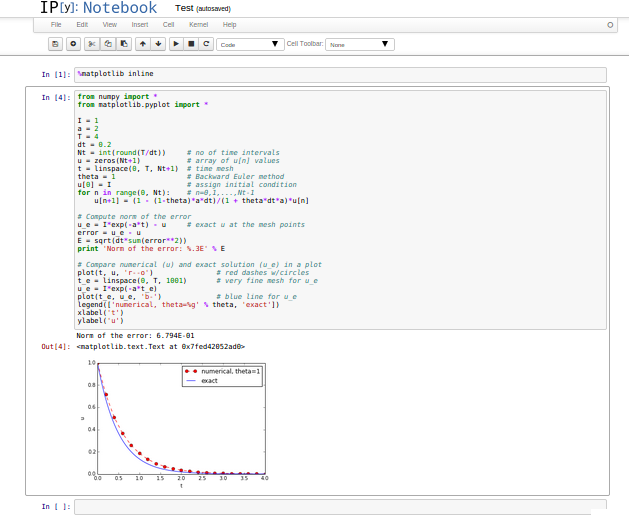
\includegraphics[width=0.8\linewidth]{fig-softeng/ipynb_flat.png}}
  \caption{
  Experimental code in a notebook. \label{softeng1:ipynb}
  }
\end{figure}
%\clearpage % flush figures softeng1:ipynb



\subsection{Prefixing imported functions by the module name}
\label{softeng1:basic:modprefix}

\index{importing modules}

Import statements of the form \texttt{from module import *} import
\emph{all} functions and variables in \texttt{module.py} into the current file.
This is often referred to as ``import star'', and
many find this convenient, but it is not considered as a good
programming style in Python.
For example, when doing

\begin{cod}{cbg_blue1}\begin{Verbatim}[numbers=none,fontsize=\fontsize{9pt}{9pt},baselinestretch=0.95,xleftmargin=2mm]
from numpy import *
from matplotlib.pyplot import *
\end{Verbatim}
\end{cod}
\noindent
we get mathematical functions like \texttt{sin} and \texttt{exp} as well as
MATLAB-style functions like \texttt{linspace} and \texttt{plot}, which can be called
by these well-known names.  Unfortunately, it sometimes becomes
confusing to know where a particular function comes from, i.e., what
modules you need to import. Is a desired function from \texttt{numpy} or
\texttt{matplotlib.pyplot}? Or is it our own function?  These questions are
easy to answer if functions in modules are prefixed by the module
name. Doing an additional \texttt{from math import *} is really crucial: now
\texttt{sin}, \texttt{cos}, and other mathematical functions are imported and their
names hide those previously imported from \texttt{numpy}.  That is, \texttt{sin} is
now a sine function that accepts a \texttt{float} argument, not an array.

Doing the import such that module functions must have a prefix
is generally recommended:

\begin{cod}{cbg_blue1}\begin{Verbatim}[numbers=none,fontsize=\fontsize{9pt}{9pt},baselinestretch=0.95,xleftmargin=2mm]
import numpy
import matplotlib.pyplot

t = numpy.linspace(0, T, Nt+1)
u_e = I*numpy.exp(-a*t)
matplotlib.pyplot.plot(t, u_e)
\end{Verbatim}
\end{cod}
\noindent

The modules \texttt{numpy} and \texttt{matplotlib.pyplot} are frequently used,
and since their full names are quite tedious to write,
two standard abbreviations
have evolved in the Python scientific computing community:

\begin{cod}{cbg_blue1}\begin{Verbatim}[numbers=none,fontsize=\fontsize{9pt}{9pt},baselinestretch=0.95,xleftmargin=2mm]
import numpy as np
import matplotlib.pyplot as plt

t = np.linspace(0, T, Nt+1)
u_e = I*np.exp(-a*t)
plt.plot(t, u_e)
\end{Verbatim}
\end{cod}
\noindent

The downside of prefixing functions by the module name is that
mathematical expressions like $e^{-at}\sin(2\pi t)$ get
cluttered with module names,
\begin{cod}{cbg_blue1}\begin{Verbatim}[numbers=none,fontsize=\fontsize{9pt}{9pt},baselinestretch=0.95,xleftmargin=2mm]
numpy.exp(-a*t)*numpy.sin(2(numpy.pi*t)
# or
np.exp(-a*t)*np.sin(2*np.pi*t)
\end{Verbatim}
\end{cod}
\noindent
Such an expression looks like \texttt{exp(-a*t)*sin(2*pi*t)} in most other
programming languages. Similarly, \texttt{np.linspace} and \texttt{plt.plot} look
less familiar to people who are used to MATLAB and who have not
adopted Python's prefix style.  Whether to do \texttt{from module import *}
or \texttt{import module} depends on personal taste and the problem at
hand. In these writings we use \texttt{from module import *} in more basic,
shorter programs where similarity with MATLAB could be an
advantage. However, in reusable modules we prefix calls to module
functions by their function name, \emph{or} do explicit import of the
needed functions:

\begin{cod}{cbg_blue1}\begin{Verbatim}[numbers=none,fontsize=\fontsize{9pt}{9pt},baselinestretch=0.95,xleftmargin=2mm]
from numpy import exp, sum, sqrt

def u_exact(t, I, a):
    return I*exp(-a*t)

error = u_exact(t, I, a) - u
E = sqrt(dt*sum(error**2))
\end{Verbatim}
\end{cod}
\noindent


\begin{notice_mdfboxadmon}[Prefixing module functions or not?]
It can be advantageous to do a combination: mathematical functions
in formulas are imported without prefix, while module functions
in general are called with a prefix. For the \texttt{numpy} package we
can do

\begin{cod}{cbg_blue1}\begin{Verbatim}[numbers=none,fontsize=\fontsize{9pt}{9pt},baselinestretch=0.95,xleftmargin=2mm]
import numpy as np
from numpy import exp, sum, sqrt
\end{Verbatim}
\end{cod}
\noindent
such that mathematical expression can apply \texttt{exp}, \texttt{sum}, and \texttt{sqrt}
and hence look as close to the mathematical formulas as possible
(without a disturbing prefix).
Other calls to \texttt{numpy} function are done with the prefix, as in
\texttt{np.linspace}.
\end{notice_mdfboxadmon}




\subsection{Implementing the numerical algorithm in a function}
\label{softeng1:basic:func}

The solution formula (\ref{softeng1:utheta}) is completely general and
should be available as a Python function \texttt{solver} with all input data as
function arguments and all output data returned to the calling code.
With this \texttt{solver} function we can solve all types of problems
(\ref{softeng1:ode})-(\ref{softeng1:u0})
by an easy-to-read one-line statement:

\begin{cod}{cbg_blue1}\begin{Verbatim}[numbers=none,fontsize=\fontsize{9pt}{9pt},baselinestretch=0.95,xleftmargin=2mm]
u, t = solver(I=1, a=2, T=4, dt=0.2, theta=0.5)
\end{Verbatim}
\end{cod}
\noindent

Refactoring the numerical method in the previous flat program
in terms of a \texttt{solver} function and prefixing calls to
module functions by the module name leads to this code:

\begin{cod}{cbg_blue1}\begin{Verbatim}[numbers=none,fontsize=\fontsize{9pt}{9pt},baselinestretch=0.95,xleftmargin=2mm]
def solver(I, a, T, dt, theta):
    """Solve u'=-a*u, u(0)=I, for t in (0,T] with steps of dt."""
    dt = float(dt)               # avoid integer division
    Nt = int(round(T/dt))        # no of time intervals
    T = Nt*dt                    # adjust T to fit time step dt
    u = np.zeros(Nt+1)           # array of u[n] values
    t = np.linspace(0, T, Nt+1)  # time mesh

    u[0] = I                  # assign initial condition
    for n in range(0, Nt):    # n=0,1,...,Nt-1
        u[n+1] = (1 - (1-theta)*a*dt)/(1 + theta*dt*a)*u[n]
    return u, t
\end{Verbatim}
\end{cod}
\noindent


\begin{notice_mdfboxadmon}[Tip: Always use a doc string to document a function!]
Python has a convention for documenting the purpose and usage of
a function in a \emph{doc string}: simply place the documentation
in a one- or multi-line triple-quoted string right after the
function header.
\end{notice_mdfboxadmon}




\begin{notice_mdfboxadmon}[Be careful with unintended integer division!]
Note that we in the \texttt{solver} function explicitly covert \texttt{dt} to a
\texttt{float} object. If not, the updating formula for \texttt{u[n+1]} may evaluate
to zero because of integer division when \texttt{theta}, \texttt{a}, and \texttt{dt} are integers!
\end{notice_mdfboxadmon}



\subsection{Do not have several versions of a code}

One of the most serious flaws in computational work is to have several
slightly different implementations of the same computational algorithms
lying around in various program files. This is very likely to happen,
because busy scientists often want to test a slight variation of a code to see
what happens. A quick copy-and-edit does the task, but such quick hacks tend
to survive. When a real correction is needed in the implementation,
it is difficult to ensure that the correction is done in all relevant files.
In fact, this is a general problem in programming, which has led to
an important principle.


\begin{notice_mdfboxadmon}[The DRY principle: Don't repeat yourself!]
When implementing a particular functionality in a computer program, make sure
this functionality and its variations are implemented in just one piece
of code. That is, if you need to revise the implementation, there should be
\emph{one and only one} place to edit. It follows that you should never
duplicate code (don't repeat yourself!), and code snippets that are
similar should be factored into one piece (function) and parameterized (by
function arguments).
\end{notice_mdfboxadmon}



The DRY principle means that our \texttt{solver} function should not be
copied to a new file if we need some modifications. Instead, we
should try to extend \texttt{solver} such that the new and old needs are
met by a single function. Sometimes this process requires a new
refactoring, but having a numerical method in one and only one place
is a great advantage.

\subsection{Making a module}
\label{softeng1:basic:module}

As soon as you start making Python functions in a program, you should
make sure the program file fulfills the requirement of a module.
This means that you can import and reuse your functions in other
programs too. For example, if our \texttt{solver} function resides in a
module file \texttt{decay.py}, another program may reuse of the
function either by

\begin{cod}{cbg_blue1}\begin{Verbatim}[numbers=none,fontsize=\fontsize{9pt}{9pt},baselinestretch=0.95,xleftmargin=2mm]
from decay import solver
u, t = solver(I=1, a=2, T=4, dt=0.2, theta=0.5)
\end{Verbatim}
\end{cod}
\noindent
or by a slightly different import statement, combined with a subsequent
prefix of the function name by the name of the module:

\begin{cod}{cbg_blue1}\begin{Verbatim}[numbers=none,fontsize=\fontsize{9pt}{9pt},baselinestretch=0.95,xleftmargin=2mm]
import decay
u, t = decay.solver(I=1, a=2, T=4, dt=0.2, theta=0.5)
\end{Verbatim}
\end{cod}
\noindent

The requirements for a program file to also qualify for a module are simple:

\begin{enumerate}
\item The filename without \texttt{.py} must be a valid Python variable name.

\item The main program must be executed (through statements or
   a function call) in the \emph{test block}.
\end{enumerate}

\noindent
The \emph{test block} is normally placed at the end of a module file:

\begin{cod}{cbg_blue1}\begin{Verbatim}[numbers=none,fontsize=\fontsize{9pt}{9pt},baselinestretch=0.95,xleftmargin=2mm]
if __name__ == '__main__':
    # Statements
\end{Verbatim}
\end{cod}
\noindent
When the module file is executed as a stand-alone program, the if test
is true and the indented statements are run. If the module file
is imported, however, \Verb!__name__! equals the module name and the test block
is not executed.

To demonstrate the difference, consider the trivial module
file \texttt{hello.py} with one function and a call to this function as main program:

\begin{pro}{cbg_blue1}{bar_blue1}\begin{Verbatim}[numbers=none,fontsize=\fontsize{9pt}{9pt},baselinestretch=0.95,xleftmargin=2mm]
def hello(arg='World!'):
    print 'Hello, ' + arg

if __name__ == '__main__':
    hello()
\end{Verbatim}
\end{pro}
\noindent
Without the test block, the code reads

\begin{pro}{cbg_blue1}{bar_blue1}\begin{Verbatim}[numbers=none,fontsize=\fontsize{9pt}{9pt},baselinestretch=0.95,xleftmargin=2mm]
def hello(arg='World!'):
    print 'Hello, ' + arg

hello()
\end{Verbatim}
\end{pro}
\noindent
With this latter version of the file, any attempt to import \texttt{hello}
will, at the same time, execute the call \texttt{hello()} and hence write
``Hello, World!'' to the screen.  Such output is not desired when
importing a module!  To make import and execution of code independent
for another program that wants to use the function \texttt{hello}, the module
\texttt{hello} must be written with a test block. Furthermore, running the
file itself as \texttt{python hello.py} will make the block active and lead
to the desired printing.


\begin{notice_mdfboxadmon}[All coming functions are placed in a module!]
The many functions to be explained in the following text are
put in one module file \href{{http://tinyurl.com/ofkw6kc/softeng/decay.py}}{\nolinkurl{decay.py}}.
\end{notice_mdfboxadmon}



What more than the \texttt{solver} function is needed in our \texttt{decay} module
to do everything we did in the previous, flat program?  We need import
statements for \texttt{numpy} and \texttt{matplotlib} as well as another function
for producing the plot. It can also be convenient to put the exact
solution in a Python function.  Our module \texttt{decay.py} then looks like
this:

\begin{cod}{cbg_blue1}\begin{Verbatim}[numbers=none,fontsize=\fontsize{9pt}{9pt},baselinestretch=0.95,xleftmargin=2mm]
import numpy as np
import matplotlib.pyplot as plt

def solver(I, a, T, dt, theta):
    ...

def u_exact(t, I, a):
    return I*np.exp(-a*t)

def experiment_compare_numerical_and_exact():
    I = 1;  a = 2;  T = 4;  dt = 0.4;  theta = 1
    u, t = solver(I, a, T, dt, theta)

    t_e = np.linspace(0, T, 1001)       # very fine mesh for u_e
    u_e = u_exact(t_e, I, a)

    plt.plot(t,   u,   'r--o')       # dashed red line with circles
    plt.plot(t_e, u_e, 'b-')         # blue line for u_e
    plt.legend(['numerical, theta=%g' % theta, 'exact'])
    plt.xlabel('t')
    plt.ylabel('u')
    plotfile = 'tmp'
    plt.savefig(plotfile + '.png');  plt.savefig(plotfile + '.pdf')

    error = u_exact(t, I, a) - u
    E = np.sqrt(dt*np.sum(error**2))
    print 'Error norm:', E

if __name__ == '__main__':
    experiment_compare_numerical_and_exact()
\end{Verbatim}
\end{cod}
\noindent
We could consider doing \texttt{from numpy import exp, sqrt, sum} to make
the mathematical expressions with these functions closer to the
mathematical formulas, but here we employed the prefix since the
formulas are so simple and easy to read.

This module file does exactly the same as the previous, flat program,
but now it becomes much easier to extend the code with more functions
that produce other plots, other experiments, etc. Even more important, though,
is that the numerical
algorithm is coded and tested once and for all in the \texttt{solver}
function, and any need to solve the mathematical problem is a matter
of one function call.
% (not copying initialization statements and a loop
% to a new program for ad hoc editing!).


\subsection{Example on extending the module code}
\label{softeng1:basic:experiment2}

Let us specifically demonstrate one extension of the flat program in
Section~\ref{softeng1:basic:impl1} that would require substantial
editing of the flat code (Section~\ref{softeng1:basic:impl2}), while in
a structured module (Section~\ref{softeng1:basic:module}), we can
simply add a new function without affecting the existing code.

Our example that illustrates the extension
is to make a comparison between the numerical solutions
for various schemes ($\theta$ values) and the exact solution:



% inline figure
\centerline{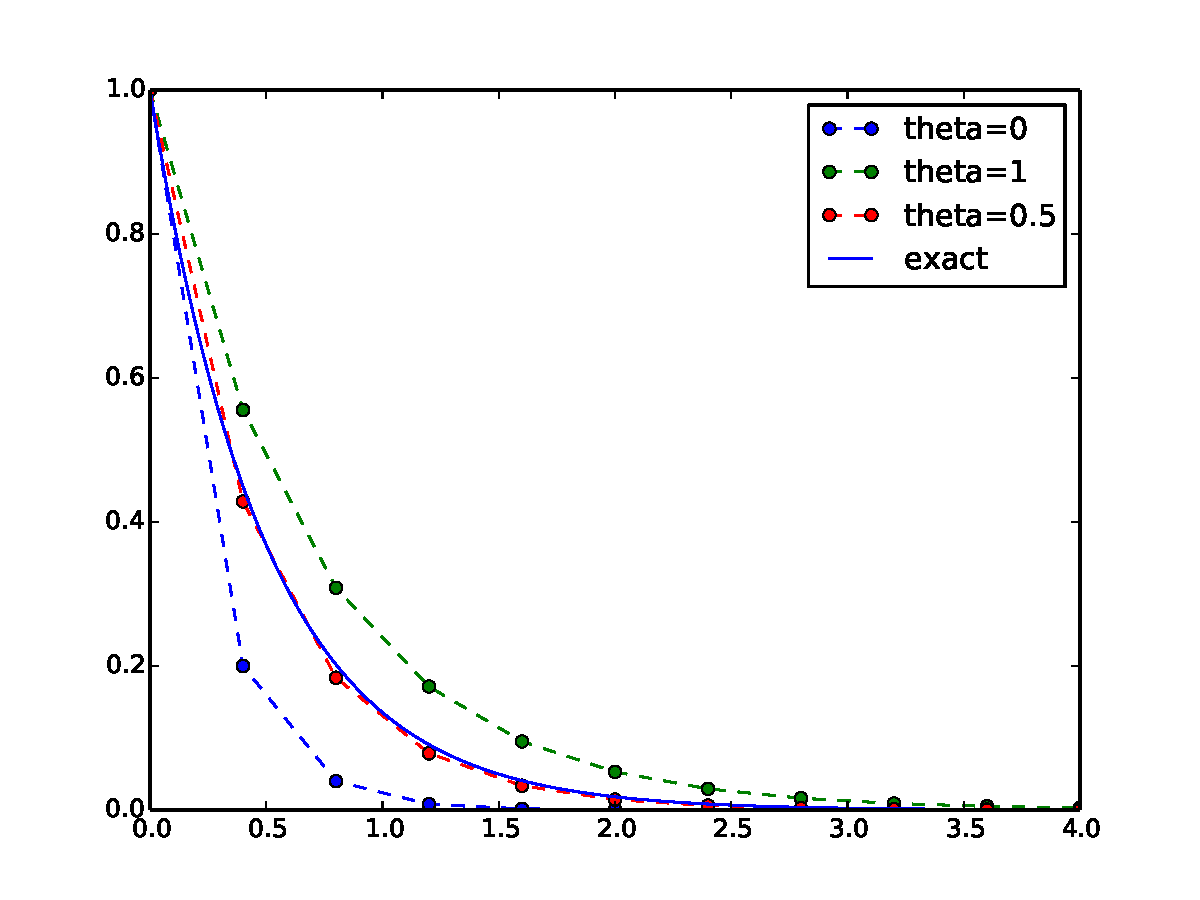
\includegraphics[width=0.7\linewidth]{fig-softeng/compare.pdf}}




\begin{question_mdfboxadmon}[Wait a minute!]
Look at the flat program in
Section~\ref{softeng1:basic:impl1},
and try to imagine which edits that are required to solve this new problem.
\end{question_mdfboxadmon}



With the \texttt{solver} function at hand, we can simply create a function
with a loop over \texttt{theta} values and add the necessary plot statements:

\begin{cod}{cbg_blue1}\begin{Verbatim}[numbers=none,fontsize=\fontsize{9pt}{9pt},baselinestretch=0.95,xleftmargin=2mm]
def experiment_compare_schemes():
    """Compare theta=0,1,0.5 in the same plot."""
    I = 1;  a = 2;  T = 4;  dt = 0.4
    legends = []
    for theta in [0, 1, 0.5]:
        u, t = solver(I, a, T, dt, theta)
        plt.plot(t, u, '--o')
        legends.append('theta=%g' % theta)
    t_e = np.linspace(0, T, 1001)        # very fine mesh for u_e
    u_e = u_exact(t_e, I, a)
    plt.plot(t_e, u_e, 'b-')
    legends.append('exact')
    plt.legend(legends, loc='upper right')
    plotfile = 'tmp'
    plt.savefig(plotfile + '.png');  plt.savefig(plotfile + '.pdf')
\end{Verbatim}
\end{cod}
\noindent

A call to this \Verb!experiment_compare_schemes! function must be placed
in the test block, or you can run the program from IPython instead:

\begin{cod}{cbg_blue1}\begin{Verbatim}[numbers=none,fontsize=\fontsize{9pt}{9pt},baselinestretch=0.95,xleftmargin=2mm]
In[1]: from decay import *

In[2]: experiment_compare_schemes()
\end{Verbatim}
\end{cod}
\noindent

We do not present how the flat program from
Section~\ref{softeng1:basic:impl2} must be refactored to produce the
desired plots, but simply state that the danger of introducing bugs
is significantly larger than when just writing an additional function
in the \texttt{decay} module.

\subsection{Documenting functions and modules}
\label{softeng1:basic:docstring}

We have already emphasized the importance of documenting functions with
a doc string (see Section~\ref{softeng1:basic:func}). Now it is time
to show how doc strings should be structured in order to take advantage
of the documentation utilities in the \texttt{numpy} module. The idea is
to follow a convention that in itself makes a good pure text doc string
in the terminal window
and at the same time can be translated to beautiful HTML manuals for
the web.

The conventions for \texttt{numpy} style doc strings are well
\href{{https://github.com/numpy/numpy/blob/master/doc/HOWTO_DOCUMENT.rst.txt}}{documented}, so here we just present a basic example that the reader can adopt.
Input arguments to a function are listed under the heading \texttt{Parameters},
while returned values are listed under \texttt{Returns}. It is a good idea to
also add an \texttt{Examples} section on the usage of the function.
More complicated software may have additional sections, see \texttt{pydoc numpy.load}
for an example. The markup language available for doc strings is
Sphinx-extended reStructuredText. The example below shows typical
constructs: 1) how inline
mathematics is written with the \texttt{:math:} directive, 2) how arguments
to the functions are referred to using single backticks
(inline monospace font for code applies double backticks), and 3) how
arguments and return values are listed with types and explanation.

\begin{cod}{cbg_blue1}\begin{Verbatim}[numbers=none,fontsize=\fontsize{9pt}{9pt},baselinestretch=0.95,xleftmargin=2mm]
def solver(I, a, T, dt, theta):
    """
    Solve :math:`u'=-au` with :math:`u(0)=I` for :math:`t \in (0,T]`
    with steps of `dt` and the method implied by `theta`.

    Parameters
    ----------
    I: float
        Initial condition.
    a: float
        Parameter in the differential equation.
    T: float
        Total simulation time.
    theta: float, int
        Parameter in the numerical scheme. 0 gives
        Forward Euler, 1 Backward Euler, and 0.5
        the centered Crank-Nicolson scheme.

    Returns
    -------
    `u`: array
        Solution array.
    `t`: array
        Array with time points corresponding to `u`.

    Examples
    --------
    Solve :math:`u' = -\\frac{1}{2}u, u(0)=1.5`
    with the Crank-Nicolson method:

    >>> u, t = solver(I=1.5, a=0.5, T=9, theta=0.5)
    >>> import matplotlib.pyplot as plt
    >>> plt.plot(t, u)
    >>> plt.show()
    """
\end{Verbatim}
\end{cod}
\noindent
If you follow such doc string conventions in your software, you can
easily produce nice manuals that meet the standard expected within
the Python scientific computing community.


\href{{http://sphinx-doc.org/}}{Sphinx} requires quite a number of manual steps to
prepare a manual, so it is
recommended to use a \href{{http://tinyurl.com/ofkw6kc/softeng/make_sphinx_api.py}}{premade script} to automate the steps. (By default,
the script generates documentation for all \texttt{*.py} files in the
current directory.
You need to do a \texttt{pip install} of \texttt{sphinx} and \texttt{numpydoc} to make the
script work.)
Figure~\ref{softeng1:basic:docstring:fig} provides an example of what
the above doc strings look like when Sphinx has transformed them to HTML.


\begin{figure}[!ht]  % softeng1:basic:docstring:fig
  \centerline{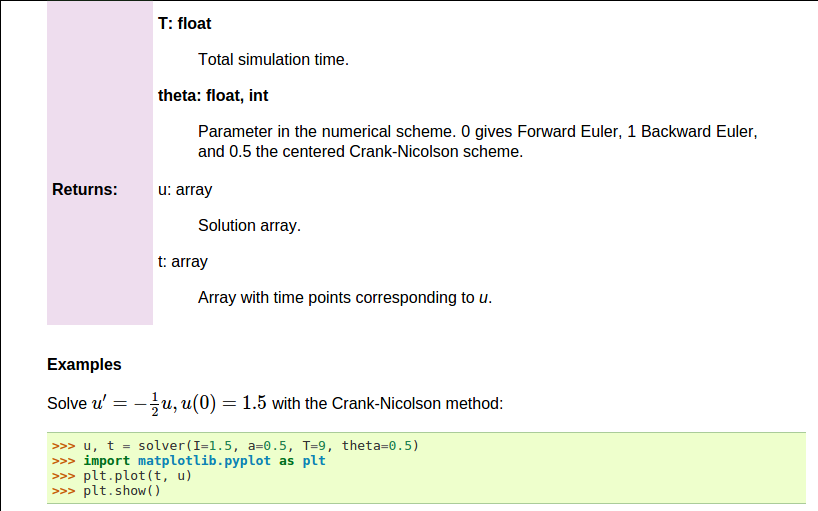
\includegraphics[width=0.8\linewidth]{fig-softeng/selfdoc_numpy.png}}
  \caption{
  Example on Sphinx API manual in HTML. \label{softeng1:basic:docstring:fig}
  }
\end{figure}
%\clearpage % flush figures softeng1:basic:docstring:fig


\subsection{Logging intermediate results}
\label{softeng1:basic:logging}

\index{logging@{\rm\texttt{logging}} module}
\index{logger}
\index{debugging}

Sometimes one may wish that a simulation program could write out
intermediate results for inspection. This could be accomplished by
a (global) \texttt{verbose} variable and code like

\begin{cod}{cbg_blue1}\begin{Verbatim}[numbers=none,fontsize=\fontsize{9pt}{9pt},baselinestretch=0.95,xleftmargin=2mm]
if verbose >= 2:
    print 'u[%d]=%g' % (i, u[i])
\end{Verbatim}
\end{cod}
\noindent
The professional way to do report intermediate results and problems is,
however, to use a \emph{logger}. This is an object that writes messages
to a log file. The messages are classified as debug, info, and warning.

\paragraph{Introductory example.}
Here is a simple example using defining a logger, using Python's \texttt{logging}
module:

\begin{pro}{cbg_blue1}{bar_blue1}\begin{Verbatim}[numbers=none,fontsize=\fontsize{9pt}{9pt},baselinestretch=0.95,xleftmargin=2mm]
import logging
logging.basicConfig(
    filename='myprog.log', filemode='w', level=logging.WARNING,
    format='%(asctime)s - %(levelname)s - %(message)s',
    datefmt='%m/%d/%Y %I:%M:%S %p')
logging.info('Here is some general info.')
logging.warning('Here is a warning.')
logging.debug('Here is some debugging info.')
logging.critical('Dividing by zero!')
logging.error('Encountered an error.')
\end{Verbatim}
\end{pro}
\noindent
Running this program gives the following output in the log file \texttt{myprog.log}:

\begin{cod}{cbg_blue1}\begin{Verbatim}[numbers=none,fontsize=\fontsize{9pt}{9pt},baselinestretch=0.95,xleftmargin=2mm]
09/26/2015 09:25:10 AM - INFO - Here is some general info.
09/26/2015 09:25:10 AM - WARNING - Here is a warning.
09/26/2015 09:25:10 AM - CRITICAL - Dividing by zero!
09/26/2015 09:25:10 AM - ERROR - Encountered an error.
\end{Verbatim}
\end{cod}
\noindent
The logger has different \emph{levels} of messages, ordered as
\emph{critical}, \emph{error}, \emph{warning}, \emph{info}, and \emph{debug}.
The \texttt{level} argument to \texttt{logging.basicConfig} sets the level
and thereby determines what the logger will print to the file:
all messages at the specified \emph{and lower} levels are printed.
For example, in the above example we set the level to be
\emph{info}, and therefore the critical, error, warning, and info
messages were printed, but not the debug message.
Setting level to debug (\texttt{logging.DEBUG}) prints all messages,
while level \emph{critical} prints only the critical messages.

The \texttt{filemode} argument is set to \texttt{w} such that any existing
log file is overwritten (the default is \texttt{a}, which means append
new messages to an existing log file, but this is seldom what
you want in mathematical computations).

The messages are preceded by the date and time and the level of
the message. This output is governed by the \texttt{format} argument:
\texttt{asctime} is the date and time, \texttt{levelname} is the name of
the message level, and \texttt{message} is the message itself.
Setting \Verb!format='%(message)s'! ensures that just the message and
nothing more is printed on each line. The \texttt{datefmt} string
specifies the formatting of the date and time, using the
rules of the \href{{https://docs.python.org/2/library/time.html#time.strftime}}{\nolinkurl{time.strftime}} function.

\paragraph{Using a logger in our solver function.}
Let us let a logger write out intermediate results and some debugging
results in the \texttt{solver} function. Such messages are useful for
monitoring the simulation and for debugging it, respectively.

\begin{cod}{cbg_blue1}\begin{Verbatim}[numbers=none,fontsize=\fontsize{9pt}{9pt},baselinestretch=0.95,xleftmargin=2mm]
import logging
logging.basicConfig(
    filename='decay.log', filemode='w', level=logging.DEBUG,
    format='%(asctime)s - %(levelname)s - %(message)s',
    datefmt='%Y.%m.%d %I:%M:%S %p')

def solver_with_logging(I, a, T, dt, theta):
    """Solve u'=-a*u, u(0)=I, for t in (0,T] with steps of dt."""
    dt = float(dt)               # avoid integer division
    Nt = int(round(T/dt))        # no of time intervals
    T = Nt*dt                    # adjust T to fit time step dt
    u = np.zeros(Nt+1)           # array of u[n] values
    t = np.linspace(0, T, Nt+1)  # time mesh
    logging.debug('solver: dt=%g, Nt=%g, T=%g' % (dt, Nt, T))

    u[0] = I                  # assign initial condition
    for n in range(0, Nt):    # n=0,1,...,Nt-1
        u[n+1] = (1 - (1-theta)*a*dt)/(1 + theta*dt*a)*u[n]

        logging.info('u[%d]=%g' % (n, u[n]))
        logging.debug('1 - (1-theta)*a*dt: %g, %s' %
                      (1-(1-theta)*a*dt,
                       str(type(1-(1-theta)*a*dt))[7:-2]))
        logging.debug('1 + theta*dt*a: %g, %s' %
                      (1 + theta*dt*a,
                       str(type(1 + theta*dt*a))[7:-2]))
    return u, t
\end{Verbatim}
\end{cod}
\noindent
We can run this new solver function in a shell:

\begin{cod}{cbg_blue1}\begin{Verbatim}[numbers=none,fontsize=\fontsize{9pt}{9pt},baselinestretch=0.95,xleftmargin=2mm]
>>> import decay
>>> u, t = decay.solver_with_logging(I=1, a=0.5, T=10, \ 
           dt=0.5, theta=0.5)
\end{Verbatim}
\end{cod}
\noindent
During this execution, each logging message is appended to the log file.
Suppose we add some pause (\texttt{time.sleep(2)}) at each time level such that
the execution takes some time. In another terminal window we can then
monitor the evolution of \texttt{decay.log} and the simulation
by the \texttt{tail -f} Unix command:

\begin{cod}{cbg_blue1}\begin{Verbatim}[numbers=none,fontsize=\fontsize{9pt}{9pt},baselinestretch=0.95,xleftmargin=2mm]
Terminal> tail -f decay.log
2015.09.26 05:37:41 AM - INFO - u[0]=1
2015.09.26 05:37:41 AM - INFO - u[1]=0.777778
2015.09.26 05:37:41 AM - INFO - u[2]=0.604938
2015.09.26 05:37:41 AM - INFO - u[3]=0.470508
2015.09.26 05:37:41 AM - INFO - u[4]=0.36595
2015.09.26 05:37:41 AM - INFO - u[5]=0.284628
\end{Verbatim}
\end{cod}
\noindent
Especially in simulation where each time step demands considerable
CPU time (minutes, hours), it can be handy to monitor such a log file
to see the evolution of the simulation.

If we want to look more closely into the numerator and denominator of
the formula for $u^{n+1}$, we can change the logging level to
\texttt{level=logging.DEBUG} and get output in \texttt{decay.log} like

\begin{cod}{cbg_blue1}\begin{Verbatim}[numbers=none,fontsize=\fontsize{9pt}{9pt},baselinestretch=0.95,xleftmargin=2mm]
2015.09.26 05:40:01 AM - DEBUG - solver: dt=0.5, Nt=20, T=10
2015.09.26 05:40:01 AM - INFO - u[0]=1
2015.09.26 05:40:01 AM - DEBUG - 1 - (1-theta)*a*dt: 0.875, float
2015.09.26 05:40:01 AM - DEBUG - 1 + theta*dt*a: 1.125, float
2015.09.26 05:40:01 AM - INFO - u[1]=0.777778
2015.09.26 05:40:01 AM - DEBUG - 1 - (1-theta)*a*dt: 0.875, float
2015.09.26 05:40:01 AM - DEBUG - 1 + theta*dt*a: 1.125, float
2015.09.26 05:40:01 AM - INFO - u[2]=0.604938
2015.09.26 05:40:01 AM - DEBUG - 1 - (1-theta)*a*dt: 0.875, float
2015.09.26 05:40:01 AM - DEBUG - 1 + theta*dt*a: 1.125, float
2015.09.26 05:40:01 AM - INFO - u[3]=0.470508
2015.09.26 05:40:01 AM - DEBUG - 1 - (1-theta)*a*dt: 0.875, float
2015.09.26 05:40:01 AM - DEBUG - 1 + theta*dt*a: 1.125, float
2015.09.26 05:40:01 AM - INFO - u[4]=0.36595
2015.09.26 05:40:01 AM - DEBUG - 1 - (1-theta)*a*dt: 0.875, float
2015.09.26 05:40:01 AM - DEBUG - 1 + theta*dt*a: 1.125, float
\end{Verbatim}
\end{cod}
\noindent



\section{User interfaces}
\label{softeng1:basic:UI}

It is good programming practice to let programs read input from
some \emph{user interface}, rather than requiring users to \emph{edit}
parameter values in the source code. With effective user interfaces
it becomes easier and safer to apply the code for scientific investigations and
in particular to automate large-scale investigations by other programs
(see Section~\ref{softeng1:experiments}).

Reading input data can be done in many ways. We have to decide on the
functionality of the user interface, i.e., how we want to operate the
program when providing input. Thereafter, we use appropriate tools to
implement the particular user interface. There are four basic types
of user interface, listed here according to implementational
complexity, from lowest to highest:

\begin{enumerate}
\item Questions and answers in the terminal window

\item Command-line arguments

\item Reading data from files

\item Graphical user interfaces (GUIs)
\end{enumerate}

\noindent
Personal preferences of user interfaces differ substantially, and it is
difficult to present recommendations or pros and cons.
Alternatives 2 and 4 are most popular and will be addressed next.
The goal is to make it easy for the user to
set physical and numerical parameters in
our \texttt{decay.py} program. However, we use  a little toy program, called
\texttt{prog.py}, as introductory
example:

\begin{pro}{cbg_blue1}{bar_blue1}\begin{Verbatim}[numbers=none,fontsize=\fontsize{9pt}{9pt},baselinestretch=0.95,xleftmargin=2mm]
delta = 0.5
p = 2
from math import exp
result = delta*exp(-p)
print result
\end{Verbatim}
\end{pro}
\noindent
The essential content is that \texttt{prog.py} has two input parameters: \texttt{delta}
and \texttt{p}. A user interface will replace the first two assignments to
\texttt{delta} and \texttt{p}.

\subsection{Command-line arguments}

The command-line arguments are all the words that appear on the
command line after the program name. Running a program \texttt{prog.py}
as \texttt{python prog.py arg1 arg2} means that there are two command-line arguments
(separated by white space): \texttt{arg1} and \texttt{arg2}.
Python stores all command-line arguments in
a special list \texttt{sys.argv}. (The name \texttt{argv} stems from the C language and
stands for ``argument values''. In C there is also an integer variable
called \texttt{argc} reflecting the number of arguments, or ``argument counter''.
A lot of programming languages have adopted the variable name \texttt{argv} for
the command-line arguments.)
Here is an example on a
program \Verb!what_is_sys_argv.py! that can show us what the command-line arguments
are

\begin{pro}{cbg_blue1}{bar_blue1}\begin{Verbatim}[numbers=none,fontsize=\fontsize{9pt}{9pt},baselinestretch=0.95,xleftmargin=2mm]
import sys
print sys.argv
\end{Verbatim}
\end{pro}
\noindent
A sample run goes like

\begin{Verbatim}[frame=lines,label=\fbox{{\tiny Terminal}},framesep=2.5mm,framerule=0.7pt,fontsize=\fontsize{9pt}{9pt}]
Terminal> python what_is_sys_argv.py 5.0 'two words' -1E+4
['what_is_sys_argv.py', '5.0', 'two words', '-1E+4']
\end{Verbatim}
We make two observations:

\begin{itemize}
 \item \texttt{sys.argv[0]} is the name of the program,
   and the sublist \texttt{sys.argv[1:]} contains all the command-line arguments.

 \item Each command-line argument is available as a string. A conversion to
   \texttt{float} is necessary if we want to compute with the numbers 5.0 and
   $10^4$.
\end{itemize}

\noindent
There are, in principle, two ways of programming with
command-line arguments in Python:

\begin{itemize}
 \item \textbf{Positional arguments:} Decide upon a sequence of parameters
   on the command line and read
   their values directly from the \texttt{sys.argv[1:]} list.

 \item \textbf{Option-value pairs:}  Use \texttt{--option value} on
   the command line to replace the default value of an input parameter
   \texttt{option} by \texttt{value} (and utilize the \texttt{argparse.ArgumentParser} tool
   for implementation).
\end{itemize}

\noindent
Suppose we want to run some program \texttt{prog.py} with
specification of two parameters \texttt{p} and \texttt{delta} on the command line.
With positional command-line arguments we write

\begin{Verbatim}[frame=lines,label=\fbox{{\tiny Terminal}},framesep=2.5mm,framerule=0.7pt,fontsize=\fontsize{9pt}{9pt}]
Terminal> python prog.py 2 0.5
\end{Verbatim}
and must know that the first argument \texttt{2} represents \texttt{p} and the
next \texttt{0.5} is the value of \texttt{delta}.
With option-value pairs we can run

\begin{Verbatim}[frame=lines,label=\fbox{{\tiny Terminal}},framesep=2.5mm,framerule=0.7pt,fontsize=\fontsize{9pt}{9pt}]
Terminal> python prog.py --delta 0.5 --p 2
\end{Verbatim}
Now, both \texttt{p} and \texttt{delta} are supposed to have default values in the program,
so we need to specify only the parameter that is to be changed from
its default value, e.g.,

\begin{Verbatim}[frame=lines,label=\fbox{{\tiny Terminal}},framesep=2.5mm,framerule=0.7pt,fontsize=\fontsize{9pt}{9pt}]
Terminal> python prog.py --p 2         # p=2, default delta
Terminal> python prog.py --delta 0.7   # delta-0.7, default a
Terminal> python prog.py               # default a and delta
\end{Verbatim}

How do we extend the \texttt{prog.py} code for positional arguments
and option-value pairs? Positional arguments require very simple
code:

\begin{pro}{cbg_blue1}{bar_blue1}\begin{Verbatim}[numbers=none,fontsize=\fontsize{9pt}{9pt},baselinestretch=0.95,xleftmargin=2mm]
import sys
p = float(sys.argv[1])
delta = float(sys.argv[2])

from math import exp
result = delta*exp(-p)
print result
\end{Verbatim}
\end{pro}
\noindent
If the user forgets to supply two command-line arguments, Python will
raise an \texttt{IndexError} exception and produce a long error message.
To avoid that, we should use a \texttt{try-except} construction:

\begin{pro}{cbg_blue1}{bar_blue1}\begin{Verbatim}[numbers=none,fontsize=\fontsize{9pt}{9pt},baselinestretch=0.95,xleftmargin=2mm]
import sys
try:
    p = float(sys.argv[1])
    delta = float(sys.argv[2])
except IndexError:
    print 'Usage: %s p delta' % sys.argv[0]
    sys.exit(1)

from math import exp
result = delta*exp(-p)
print result
\end{Verbatim}
\end{pro}
\noindent
Using \texttt{sys.exit(1)} aborts the program. The value 1 (actually any
value different from 0) notifies the operating system that the
program failed.


\begin{warning_mdfboxadmon}[Command-line arguments are strings!]
Note that all elements in \texttt{sys.argv} are string objects.
If the values are used in mathematical computations, we need
to explicitly convert the strings to numbers.
\end{warning_mdfboxadmon}



Option-value pairs requires more programming and is actually
better explained in a more comprehensive example below.
Minimal code for our \texttt{prog.py} program reads

\begin{pro}{cbg_blue1}{bar_blue1}\begin{Verbatim}[numbers=none,fontsize=\fontsize{9pt}{9pt},baselinestretch=0.95,xleftmargin=2mm]
import argparse
parser = argparse.ArgumentParser()
parser.add_argument('--p', default=1.0)
parser.add_argument('--delta', default=0.1)

args = parser.parse_args()
p = args.p
delta = args.delta

from math import exp
result = delta*exp(-p)
print result
\end{Verbatim}
\end{pro}
\noindent
Because the default values of \texttt{delta} and \texttt{p} are float numbers,
the \texttt{args.delta} and \texttt{args.p} variables are automatically of type \texttt{float}.

Our next task is to use these basic code constructs to equip our
\texttt{decay.py} module with command-line interfaces.

\subsection{Positional command-line arguments}

\index{list comprehension}
\index{sys.argv@{\rm\texttt{sys.argv}}}
\index{command-line arguments}

For our \texttt{decay.py} module file, we want to include functionality such
that we can read $I$, $a$, $T$, $\theta$, and a range of $\Delta t$
values from the command line.  A plot is then to be made, comparing
the different numerical solutions for different $\Delta t$ values
against the exact solution. The technical details of getting the
command-line information into the program is covered in the next
two sections.

The simplest way of reading the input parameters is to
decide on their sequence on the command line and just index
the \texttt{sys.argv} list accordingly.
Say the sequence of input data for some functionality in
\texttt{decay.py} is $I$, $a$, $T$, $\theta$ followed by an
arbitrary number of $\Delta t$ values. This code extracts
these \emph{positional} command-line arguments:

\begin{cod}{cbg_blue1}\begin{Verbatim}[numbers=none,fontsize=\fontsize{9pt}{9pt},baselinestretch=0.95,xleftmargin=2mm]
def read_command_line_positional():
    if len(sys.argv) < 6:
        print 'Usage: %s I a T on/off BE/FE/CN dt1 dt2 dt3 ...' % \ 
              sys.argv[0]; sys.exit(1)  # abort

    I = float(sys.argv[1])
    a = float(sys.argv[2])
    T = float(sys.argv[3])
    theta = float(sys.argv[4])
    dt_values = [float(arg) for arg in sys.argv[5:]]

    return I, a, T, theta, dt_values
\end{Verbatim}
\end{cod}
\noindent
Note that we may use a \texttt{try-except} construction instead of the if test.

A run like

\begin{Verbatim}[frame=lines,label=\fbox{{\tiny Terminal}},framesep=2.5mm,framerule=0.7pt,fontsize=\fontsize{9pt}{9pt}]
Terminal> python decay.py 1 0.5 4 0.5 1.5 0.75 0.1
\end{Verbatim}
results in

\begin{cod}{cbg_blue1}\begin{Verbatim}[numbers=none,fontsize=\fontsize{9pt}{9pt},baselinestretch=0.95,xleftmargin=2mm]
sys.argv = ['decay.py', '1', '0.5', '4', '0.5', '1.5', '0.75', '0.1']
\end{Verbatim}
\end{cod}
\noindent
and consequently the assignments \texttt{I=1.0}, \texttt{a=0.5}, \texttt{T=4.0}, \texttt{thet=0.5},
and \Verb!dt_values = [1.5, 0.75, 0.1]!.

Instead of specifying the $\theta$ value, we could be a bit more
sophisticated and let the user write the name of the scheme:
\texttt{BE} for Backward Euler, \texttt{FE} for Forward Euler, and \texttt{CN}
for Crank-Nicolson. Then we must map this string to the proper
$\theta$ value, an operation elegantly done by a dictionary:

\begin{cod}{cbg_blue1}\begin{Verbatim}[numbers=none,fontsize=\fontsize{9pt}{9pt},baselinestretch=0.95,xleftmargin=2mm]
scheme = sys.argv[4]
scheme2theta = {'BE': 1, 'CN': 0.5, 'FE': 0}
if scheme in scheme2theta:
    theta = scheme2theta[scheme]
else:
    print 'Invalid scheme name:', scheme; sys.exit(1)
\end{Verbatim}
\end{cod}
\noindent
Now we can do

\begin{Verbatim}[frame=lines,label=\fbox{{\tiny Terminal}},framesep=2.5mm,framerule=0.7pt,fontsize=\fontsize{9pt}{9pt}]
Terminal> python decay.py 1 0.5 4 CN 1.5 0.75 0.1
\end{Verbatim}
and get `theta=0.5`in the code.


\subsection{Option-value pairs on the command line}

\index{argparse@{\rm\texttt{argparse}} (Python module)}
\index{ArgumentParser@{\rm\texttt{ArgumentParser}} (Python class)}
\index{option-value pairs (command line)}
\index{command-line arguments}
\index{reading the command line}

Now we want to specify option-value pairs on the command line,
using \texttt{--I} for \texttt{I} ($I$), \texttt{--a} for \texttt{a} ($a$), \texttt{--T} for \texttt{T} ($T$),
\texttt{--scheme} for the scheme name (\texttt{BE}, \texttt{FE}, \texttt{CN}),
and \texttt{--dt} for the sequence of \texttt{dt} ($\Delta t$) values.
Each parameter must have a sensible default value so
that we specify the option on the command line only when the default
value is not suitable. Here is a typical run:

\begin{Verbatim}[frame=lines,label=\fbox{{\tiny Terminal}},framesep=2.5mm,framerule=0.7pt,fontsize=\fontsize{9pt}{9pt}]
Terminal> python decay.py --I 2.5 --dt 0.1 0.2 0.01 --a 0.4
\end{Verbatim}
Observe the major advantage over positional command-line arguments:
the input is much easier to read and much easier to write.
With positional arguments it is easy to mess up the sequence of
the input parameters and quite challenging to detect errors too,
unless there are just a couple of arguments.

Python's \texttt{ArgumentParser} tool in the \texttt{argparse} module makes it easy
to create a professional command-line interface to any program. The
documentation of \href{{http://docs.python.org/library/argparse.html}}{\nolinkurl{ArgumentParser}} demonstrates its
versatile applications, so we shall here just list an example
containing the most basic features. It always pays off to use \texttt{ArgumentParser}
rather than trying to manually inspect and interpret option-value pairs
in \texttt{sys.argv}!

The use of \texttt{ArgumentParser} typically involves three steps:

\begin{cod}{cbg_blue1}\begin{Verbatim}[numbers=none,fontsize=\fontsize{9pt}{9pt},baselinestretch=0.95,xleftmargin=2mm]
import argparse
parser = argparse.ArgumentParser()

# Step 1: add arguments
parser.add_argument('--option_name', ...)

# Step 2: interpret the command line
args = parser.parse_args()

# Step 3: extract values
value = args.option_name
\end{Verbatim}
\end{cod}
\noindent

A function for setting up all the options is handy:

\begin{cod}{cbg_blue1}\begin{Verbatim}[numbers=none,fontsize=\fontsize{9pt}{9pt},baselinestretch=0.95,xleftmargin=2mm]
def define_command_line_options():
    import argparse
    parser = argparse.ArgumentParser()
    parser.add_argument(
        '--I', '--initial_condition', type=float,
        default=1.0, help='initial condition, u(0)',
        metavar='I')
    parser.add_argument(
        '--a', type=float, default=1.0,
        help='coefficient in ODE', metavar='a')
    parser.add_argument(
        '--T', '--stop_time', type=float,
        default=1.0, help='end time of simulation',
        metavar='T')
    parser.add_argument(
        '--scheme', type=str, default='CN',
        help='FE, BE, or CN')
    parser.add_argument(
        '--dt', '--time_step_values', type=float,
        default=[1.0], help='time step values',
        metavar='dt', nargs='+', dest='dt_values')
    return parser
\end{Verbatim}
\end{cod}
\noindent

Each command-line option is defined through the \Verb!parser.add_argument!
method\footnote{We use the expression \emph{method} here, because \texttt{parser} is a class variable and functions in classes are known as methods in Python and many other languages. Readers not familiar with class programming can just substitute this use of \emph{method} by \emph{function}.}. Alternative options, like the short \texttt{--I} and the more
explaining version \Verb!--initial_condition! can be defined. Other arguments
are \texttt{type} for the Python object type, a default value, and a help
string, which gets printed if the command-line argument \texttt{-h} or \texttt{--help} is
included. The \texttt{metavar} argument specifies the value associated with
the option when the help string is printed. For example, the option for
$I$ has this help output:

\begin{Verbatim}[frame=lines,label=\fbox{{\tiny Terminal}},framesep=2.5mm,framerule=0.7pt,fontsize=\fontsize{9pt}{9pt}]
Terminal> python decay.py -h
  ...
  --I I, --initial_condition I
                        initial condition, u(0)
  ...
\end{Verbatim}
The structure of this output is

\begin{cod}{cbg_blue1}\begin{Verbatim}[numbers=none,fontsize=\fontsize{9pt}{9pt},baselinestretch=0.95,xleftmargin=2mm]
  --I metavar, --initial_condition metavar
                        help-string
\end{Verbatim}
\end{cod}
\noindent



Finally, the \texttt{--dt} option demonstrates how to allow for more than one
value (separated by blanks) through the \texttt{nargs='+'} keyword argument.
After the command line is parsed, we get an object where the values of
the options are stored as attributes. The attribute name is specified
by the \texttt{dist} keyword argument, which for the \texttt{--dt} option is
\Verb!dt_values!. Without the \texttt{dest} argument, the value of an option \texttt{--opt}
is stored as the attribute \texttt{opt}.

The code below demonstrates how to read the command line and extract
the values for each option:

\begin{cod}{cbg_blue1}\begin{Verbatim}[numbers=none,fontsize=\fontsize{9pt}{9pt},baselinestretch=0.95,xleftmargin=2mm]
def read_command_line_argparse():
    parser = define_command_line_options()
    args = parser.parse_args()
    scheme2theta = {'BE': 1, 'CN': 0.5, 'FE': 0}
    data = (args.I, args.a, args.T, scheme2theta[args.scheme],
            args.dt_values)
    return data
\end{Verbatim}
\end{cod}
\noindent
As seen, the values of the command-line options are available as
attributes in \texttt{args}: \texttt{args.opt} holds the value of option \texttt{--opt}, unless
we used the \texttt{dest} argument (as for \Verb!--dt_values!) for specifying the
attribute name. The \texttt{args.opt} attribute has the object type specified
by \texttt{type} (\texttt{str} by default).

The making of the plot is not dependent on whether we read data from
the command line as positional arguments or option-value pairs:

\begin{cod}{cbg_blue1}\begin{Verbatim}[numbers=none,fontsize=\fontsize{9pt}{9pt},baselinestretch=0.95,xleftmargin=2mm]
def experiment_compare_dt(option_value_pairs=False):
    I, a, T, theta, dt_values = \ 
       read_command_line_argparse() if option_value_pairs else \ 
       read_command_line_positional()

    legends = []
    for dt in dt_values:
        u, t = solver(I, a, T, dt, theta)
        plt.plot(t, u)
        legends.append('dt=%g' % dt)
    t_e = np.linspace(0, T, 1001)       # very fine mesh for u_e
    u_e = u_exact(t_e, I, a)
    plt.plot(t_e, u_e, '--')
    legends.append('exact')
    plt.legend(legends, loc='upper right')
    plt.title('theta=%g' % theta)
    plotfile = 'tmp'
    plt.savefig(plotfile + '.png');  plt.savefig(plotfile + '.pdf')
\end{Verbatim}
\end{cod}
\noindent


\subsection{Creating a graphical web user interface}

The Python package \href{{https://github.com/hplgit/parampool}}{Parampool}
can be used to automatically generate a web-based \emph{graphical user interface}
(GUI) for our simulation program. Although the programming technique
dramatically simplifies the efforts to create a GUI, the forthcoming
material on equipping our \texttt{decay} module with a GUI is quite technical
and of significantly less importance than knowing how to make
a command-line interface.

\paragraph{Making a compute function.}
The first step is to identify a function
that performs the computations and that takes the necessary input
variables as arguments. This is called the \emph{compute function} in
Parampool terminology. The purpose of this function is to take
values of $I$, $a$, $T$ together with a sequence of $\Delta t$ values
and a sequence of $\theta$ and plot the numerical against the
exact solution for each pair of $(\theta, \Delta t)$.
The plots can be arranged as a table with the columns being scheme type
($\theta$ value) and the rows reflecting the discretization parameter
($\Delta t$ value). Figure~\ref{softeng1:fig:GUI} displays what the
graphical web interface may look like after results are computed
(there are $3\times 3$ plots in the GUI, but only $2\times 2$ are
visible in the figure).


\begin{figure}[!ht]  % softeng1:fig:GUI
  \centerline{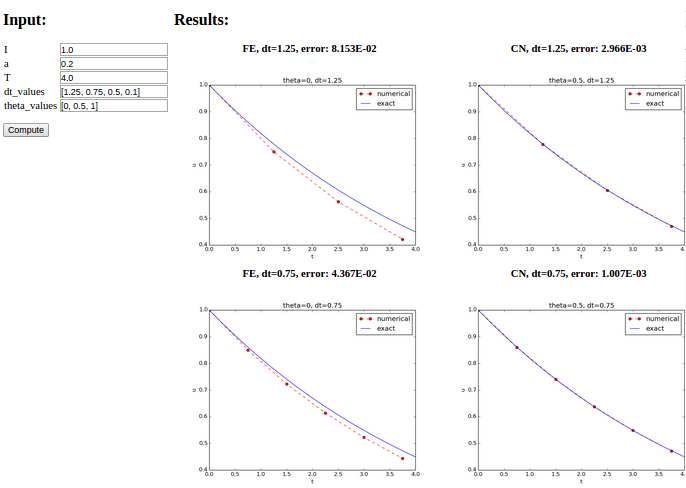
\includegraphics[width=1.0\linewidth]{fig-softeng/web_GUI.png}}
  \caption{
  Automatically generated graphical web interface. \label{softeng1:fig:GUI}
  }
\end{figure}
%\clearpage % flush figures softeng1:fig:GUI



To tell Parampool what type of input data we have,
we assign default values of the right type to all arguments in the
compute function, here called \Verb!main_GUI!:

\begin{cod}{cbg_blue1}\begin{Verbatim}[numbers=none,fontsize=\fontsize{9pt}{9pt},baselinestretch=0.95,xleftmargin=2mm]
def main_GUI(I=1.0, a=.2, T=4.0,
             dt_values=[1.25, 0.75, 0.5, 0.1],
             theta_values=[0, 0.5, 1]):
\end{Verbatim}
\end{cod}
\noindent

The compute function must return the HTML code we want for displaying
the result in a web page. Here we want to show a
table of plots.
Assume for now that the HTML code for one plot and the value of the
norm of the error can be computed by some other function \texttt{compute4web}.
The \Verb!main_GUI! function can then loop over $\Delta t$ and $\theta$
values and put each plot in an HTML table. Appropriate code goes like

\begin{cod}{cbg_blue1}\begin{Verbatim}[numbers=none,fontsize=\fontsize{9pt}{9pt},baselinestretch=0.95,xleftmargin=2mm]
def main_GUI(I=1.0, a=.2, T=4.0,
             dt_values=[1.25, 0.75, 0.5, 0.1],
             theta_values=[0, 0.5, 1]):
    # Build HTML code for web page. Arrange plots in columns
    # corresponding to the theta values, with dt down the rows
    theta2name = {0: 'FE', 1: 'BE', 0.5: 'CN'}
    html_text = '<table>\n'
    for dt in dt_values:
        html_text += '<tr>\n'
        for theta in theta_values:
            E, html = compute4web(I, a, T, dt, theta)
            html_text += """
<td>
<center><b>%s, dt=%g, error: %.3E</b></center><br>
%s
</td>
""" % (theta2name[theta], dt, E, html)
        html_text += '</tr>\n'
    html_text += '</table>\n'
    return html_text
\end{Verbatim}
\end{cod}
\noindent

Making one plot is done in \texttt{compute4web}. The statements should be
straightforward from earlier examples, but there is one new feature:
we use a tool in Parampool to embed the PNG code for a plot file
directly in an HTML image tag. The details are hidden from the
programmer, who can just rely on
relevant HTML code in the string \Verb!html_text!. The function looks like

\begin{cod}{cbg_blue1}\begin{Verbatim}[numbers=none,fontsize=\fontsize{9pt}{9pt},baselinestretch=0.95,xleftmargin=2mm]
def compute4web(I, a, T, dt, theta=0.5):
    """
    Run a case with the solver, compute error measure,
    and plot the numerical and exact solutions in a PNG
    plot whose data are embedded in an HTML image tag.
    """
    u, t = solver(I, a, T, dt, theta)
    u_e = u_exact(t, I, a)
    e = u_e - u
    E = np.sqrt(dt*np.sum(e**2))

    plt.figure()
    t_e = np.linspace(0, T, 1001)    # fine mesh for u_e
    u_e = u_exact(t_e, I, a)
    plt.plot(t,   u,   'r--o')
    plt.plot(t_e, u_e, 'b-')
    plt.legend(['numerical', 'exact'])
    plt.xlabel('t')
    plt.ylabel('u')
    plt.title('theta=%g, dt=%g' % (theta, dt))
    # Save plot to HTML img tag with PNG code as embedded data
    from parampool.utils import save_png_to_str
    html_text = save_png_to_str(plt, plotwidth=400)

    return E, html_text
\end{Verbatim}
\end{cod}
\noindent


\paragraph{Generating the user interface.}
The web GUI is automatically generated by
the following code, placed in the file \href{{http://tinyurl.com/ofkw6kc/softeng/decay_GUI_generate.py}}{\nolinkurl{decay_GUI_generate.py}}.

\begin{pro}{cbg_blue1}{bar_blue1}\begin{Verbatim}[numbers=none,fontsize=\fontsize{9pt}{9pt},baselinestretch=0.95,xleftmargin=2mm]
from parampool.generator.flask import generate
from decay import main_GUI
generate(main_GUI,
         filename_controller='decay_GUI_controller.py',
         filename_template='decay_GUI_view.py',
         filename_model='decay_GUI_model.py')
\end{Verbatim}
\end{pro}
\noindent
Running the \Verb!decay_GUI_generate.py! program results in three new
files whose names are specified in the call to \texttt{generate}:

\begin{enumerate}
 \item \Verb!decay_GUI_model.py! defines HTML widgets to be used to set
    input data in the web interface,

 \item \Verb!templates/decay_GUI_views.py! defines the layout of the web page,

 \item \Verb!decay_GUI_controller.py! runs the web application.
\end{enumerate}

\noindent
We only need to run the last program, and there is no need to look into
these files.

\paragraph{Running the web application.}
The web GUI is started by

\begin{Verbatim}[frame=lines,label=\fbox{{\tiny Terminal}},framesep=2.5mm,framerule=0.7pt,fontsize=\fontsize{9pt}{9pt}]
Terminal> python decay_GUI_controller.py
\end{Verbatim}
Open a web browser at the location \texttt{127.0.0.1:5000}. Input fields for
\texttt{I}, \texttt{a}, \texttt{T}, \Verb!dt_values!, and \Verb!theta_values! are presented.  Figure~\ref{softeng1:fig:GUI} shows a part of the resulting page if we run
with the default values for the input parameters.
With the techniques demonstrated here, one can
easily create a tailored web GUI for a particular type of application
and use it to interactively explore physical and numerical effects.

\section{Tests for verifying implementations}

Any module with functions should have a set of tests that can
check the
correctness of the implementations.
There exists
well-established procedures and corresponding tools for automating
the execution of such tests. These tools allow large test sets to be
run with a one-line command, making it easy to check that the
software still works (as far as the
tests can tell!). Here we shall illustrate two important
software testing techniques: \emph{doctest} and \emph{unit testing}.
The first one is Python specific, while unit testing is the dominating
test technique in the software industry today.

\subsection{Doctests}

\index{doctests}
\index{software testing!doctests}

A doc string, the first string after the function header, is used to
document the purpose of functions and their arguments
(see Section~\ref{softeng1:basic:func}). Very often it
is instructive to include an example in the doc string
on how to use the function.
Interactive examples in the Python shell are most illustrative as
we can see the output resulting from the statements and expressions.
For example,
in the \texttt{solver} function, we can include an example on calling
this function and printing the computed \texttt{u} and \texttt{t} arrays:

\begin{cod}{cbg_blue1}\begin{Verbatim}[numbers=none,fontsize=\fontsize{9pt}{9pt},baselinestretch=0.95,xleftmargin=2mm]
def solver(I, a, T, dt, theta):
    """
    Solve u'=-a*u, u(0)=I, for t in (0,T] with steps of dt.


    >>> u, t = solver(I=0.8, a=1.2, T=1.5, dt=0.5, theta=0.5)
    >>> for n in range(len(t)):
    ...     print 't=%.1f, u=%.14f' % (t[n], u[n])
    t=0.0, u=0.80000000000000
    t=0.5, u=0.43076923076923
    t=1.0, u=0.23195266272189
    t=1.5, u=0.12489758761948
    """
    ...
\end{Verbatim}
\end{cod}
\noindent

When such interactive demonstrations are inserted in doc strings,
Python's \href{{http://docs.python.org/library/doctest.html}}{\nolinkurl{doctest}}
module can be used to automate running all commands
in interactive sessions and compare new output with the output
appearing in the doc string.  All we have to do in the current example
is to run the module file \texttt{decay.py} with

\begin{cod}{cbg_blue1}\begin{Verbatim}[numbers=none,fontsize=\fontsize{9pt}{9pt},baselinestretch=0.95,xleftmargin=2mm]
Terminal> python -m doctest decay.py
\end{Verbatim}
\end{cod}
\noindent
This command imports the \texttt{doctest} module, which runs all
doctests found in the file and reports discrepancies between
expected and computed output.
Alternatively, the test block in a module may run all doctests
by

\begin{cod}{cbg_blue1}\begin{Verbatim}[numbers=none,fontsize=\fontsize{9pt}{9pt},baselinestretch=0.95,xleftmargin=2mm]
if __name__ == '__main__':
    import doctest
    doctest.testmod()
\end{Verbatim}
\end{cod}
\noindent
Doctests can also be embedded in nose/pytest unit tests
as explained in the next section.


\begin{warning_mdfboxadmon}[Doctests prevent command-line arguments!]
No additional command-line argument is allowed when running doctests.
If your program relies on command-line input, make sure the doctests
can be run \emph{without} such input on the command line.

However, you can simulate command-line input by filling \texttt{sys.argv}
with values, e.g.,

\begin{cod}{cbg_blue1}\begin{Verbatim}[numbers=none,fontsize=\fontsize{9pt}{9pt},baselinestretch=0.95,xleftmargin=2mm]
import sys; sys.argv = '--I 1.0 --a 5'.split()
\end{Verbatim}
\end{cod}
\noindent
\end{warning_mdfboxadmon}



The execution command above will report any problem if a test fails.
As an illustration, let us alter the \texttt{u} value at \texttt{t=1.5} in
the output of the doctest by replacing the last digit \texttt{8} by \texttt{7}.
This edit triggers a report:

\begin{Verbatim}[frame=lines,label=\fbox{{\tiny Terminal}},framesep=2.5mm,framerule=0.7pt,fontsize=\fontsize{9pt}{9pt}]
Terminal> python -m doctest decay.py
********************************************************
File "decay.py", line ...
Failed example:
    for n in range(len(t)):
        print 't=%.1f, u=%.14f' % (t[n], u[n])
Expected:
    t=0.0, u=0.80000000000000
    t=0.5, u=0.43076923076923
    t=1.0, u=0.23195266272189
    t=1.5, u=0.12489758761948
Got:
    t=0.0, u=0.80000000000000
    t=0.5, u=0.43076923076923
    t=1.0, u=0.23195266272189
    t=1.5, u=0.12489758761947
\end{Verbatim}


\begin{warning_mdfboxadmon}[Pay attention to the number of digits in doctest results!]
Note that in the output of \texttt{t} and \texttt{u} we write \texttt{u} with 14 digits.
Writing all 16 digits is not a good idea: if the tests are run on
different hardware, round-off errors might be different, and
the \texttt{doctest} module detects that the numbers are not precisely the same
and reports failures. In the present application, where $0 < u(t) \leq 0.8$,
we expect round-off errors to be of size $10^{-16}$, so comparing 15
digits would probably be reliable, but we compare 14 to be on the
safe side. On the other hand, comparing a small number of digits may
hide software errors.
\end{warning_mdfboxadmon}



Doctests are highly encouraged as they do two things: 1) demonstrate
how a function is used and 2) test that the function works.


\subsection{Unit tests and test functions}

\index{nose@{\rm\texttt{nose}} tests}
\index{pytest@{\rm\texttt{pytest}} tests}
\index{unit testing}
\index{software testing!nose}
\index{software testing!pytest}

The unit testing technique consists of identifying smaller units
of code and writing one or more tests for
each unit. One unit can typically be a function.
Each test should, ideally, not depend on the outcome of
other tests. The recommended practice is actually to
design and write the unit tests first and \emph{then} implement the functions!

In scientific computing it is not always obvious how to best perform
unit testing. The units are naturally larger than in non-scientific
software. Very often the solution procedure of a mathematical problem
identifies a unit, such as our \texttt{solver} function.

\index{test function}
\index{software testing!test function}

\paragraph{Two Python test frameworks: nose and pytest.}
Python offers two very easy-to-use software frameworks for implementing
unit tests: nose and pytest. These work (almost) in the same way,
but our recommendation is to go for pytest.

\paragraph{Test function requirements.}
For a test to qualify as a \emph{test function} in nose or pytest, three
rules must be followed:

\begin{enumerate}
 \item The function name must start with \Verb!test_!.

 \item Function arguments are not allowed.

 \item An \texttt{AssertionError} exception must be raised if the test fails.
\end{enumerate}

\noindent
A specific example might be illustrative before proceeding.
We have the following function that we want to test:

\begin{cod}{cbg_blue1}\begin{Verbatim}[numbers=none,fontsize=\fontsize{9pt}{9pt},baselinestretch=0.95,xleftmargin=2mm]
def double(n):
    return 2*n
\end{Verbatim}
\end{cod}
\noindent
The corresponding test function could, in principle, have been written
as

\begin{cod}{cbg_blue1}\begin{Verbatim}[numbers=none,fontsize=\fontsize{9pt}{9pt},baselinestretch=0.95,xleftmargin=2mm]
def test_double():
    """Test that double(n) works for one specific n."""
    n = 4
    expected = 2*4
    computed = double(4)
    if expected != computed:
        raise AssertionError
\end{Verbatim}
\end{cod}
\noindent
The last two lines, however, are never written like this in test functions.
Instead, Python's \texttt{assert} statement is used: \texttt{assert success, msg}, where
\texttt{success} is a boolean variable, which is \texttt{False} if the test fails, and
\texttt{msg} is \emph{an optional} message string that is printed when the test fails.
A better version of the test function is therefore

\begin{cod}{cbg_blue1}\begin{Verbatim}[numbers=none,fontsize=\fontsize{9pt}{9pt},baselinestretch=0.95,xleftmargin=2mm]
def test_double():
    """Test that double(n) works for one specific n."""
    n = 4
    expected = 2*4
    computed = double(4)
    msg = 'expected %g, computed %g' % (expected, computed)
    success = expected == computed
    assert success, msg
\end{Verbatim}
\end{cod}
\noindent

\paragraph{Comparison of real numbers.}
Because of the finite precision arithmetics on a computer, which gives
rise to round-off errors, the \texttt{==} operator is not suitable for
checking whether two real numbers are equal. Obviously, this principle
also applies to tests in test functions.
We must therefore replace \texttt{a == b} by a comparison
based on a tolerance \texttt{tol}: \texttt{abs(a-b) < tol}. The next example illustrates
the problem and its solution.

Here is a slightly different function that
we want to test:

\begin{cod}{cbg_blue1}\begin{Verbatim}[numbers=none,fontsize=\fontsize{9pt}{9pt},baselinestretch=0.95,xleftmargin=2mm]
def third(x):
    return x/3.
\end{Verbatim}
\end{cod}
\noindent
We write a test function where the expected result is computed as
$\frac{1}{3}x$ rather than $x/3$:

\begin{cod}{cbg_blue1}\begin{Verbatim}[numbers=none,fontsize=\fontsize{9pt}{9pt},baselinestretch=0.95,xleftmargin=2mm]
def test_third():
    """Check that third(x) works for many x values."""
    for x in np.linspace(0, 1, 21):
        expected = (1/3.0)*x
        computed = third(x)
        success = expected == computed
        assert success
\end{Verbatim}
\end{cod}
\noindent
This \Verb!test_third! function executes silently, i.e., no failure,
until \texttt{x} becomes 0.15. Then round-off errors make the \texttt{==} comparison
\texttt{False}. In fact, seven of the \texttt{x} values above face this problem.
The solution is to compare \texttt{expected} and \texttt{computed}
with a small tolerance:

\begin{cod}{cbg_blue1}\begin{Verbatim}[numbers=none,fontsize=\fontsize{9pt}{9pt},baselinestretch=0.95,xleftmargin=2mm]
def test_third():
    """Check that third(x) works for many x values."""
    for x in np.linspace(0, 1, 21):
        expected = (1/3.)*x
        computed = third(x)
        tol = 1E-15
        success = abs(expected - computed) < tol
        assert success
\end{Verbatim}
\end{cod}
\noindent


\begin{notice_mdfboxadmon}[Always compare real numbers with a tolerance!]
Real numbers should never be compared with the \texttt{==} operator, but always
with the absolute value of the difference and a tolerance.
So, replace \texttt{a == b}, if \texttt{a} and/or \texttt{b} is \texttt{float}, by

\begin{cod}{cbg_blue1}\begin{Verbatim}[numbers=none,fontsize=\fontsize{9pt}{9pt},baselinestretch=0.95,xleftmargin=2mm]
tol = 1E-14
abs(a - b) < tol
\end{Verbatim}
\end{cod}
\noindent
The suitable size of \texttt{tol} depends on the size of \texttt{a} and \texttt{b}
(see Problem~\ref{softeng1:exer:tol}).
\end{notice_mdfboxadmon}



\paragraph{Special assert functions from nose.}
Test frameworks often contain more tailored
\emph{assert functions} that can be called instead of using the \texttt{assert}
statement. For example, comparing two objects within
a tolerance, as in the present
case, can be done by the \Verb!assert_almost_equal! from the nose
framework:

\begin{cod}{cbg_blue1}\begin{Verbatim}[numbers=none,fontsize=\fontsize{9pt}{9pt},baselinestretch=0.95,xleftmargin=2mm]
import nose.tools as nt

def test_third():
    x = 0.15
    expected = (1/3.)*x
    computed = third(x)
    nt.assert_almost_equal(
        expected, computed, delta=1E-15,
        msg='diff=%.17E' % (expected - computed))
\end{Verbatim}
\end{cod}
\noindent

Whether to use the plain \texttt{assert} statement with a comparison based on
a tolerance or to use the ready-made function \Verb!assert_almost_equal!
depends on the programmer's preference. The examples used in the
documentation of the pytest framework stick to the plain \texttt{assert}
statement.

\paragraph{Locating test functions.}
Test functions can reside in a module together with the functions they
are supposed to verify, or the test functions can be collected in
separate files having names starting with \texttt{test}. Actually,
nose and pytest can recursively run all test functions
in all \texttt{test*.py}
files in the current directory, as well as in all subdirectories!

The \href{{http://tinyurl.com/ofkw6kc/softeng/decay.py}}{\nolinkurl{decay.py}} module file features
test functions in the module, but we could equally well have made
a subdirectory \texttt{tests} and put the test functions in
\href{{http://tinyurl.com/ofkw6kc/softeng/tests/test_decay.py}}{\nolinkurl{tests/test_decay.py}}.

\paragraph{Running tests.}
To run all test functions in the file \texttt{decay.py} do

\begin{Verbatim}[frame=lines,label=\fbox{{\tiny Terminal}},framesep=2.5mm,framerule=0.7pt,fontsize=\fontsize{9pt}{9pt}]
Terminal> nosetests -s -v decay.py
Terminal> py.test -s -v decay.py
\end{Verbatim}
The \texttt{-s} option ensures that output from the test functions is printed
in the terminal window, while \texttt{-v} prints the outcome of each individual
test function.

Alternatively, if the test functions are located in some separate
\texttt{test*.py} files,
we can just write

\begin{Verbatim}[frame=lines,label=\fbox{{\tiny Terminal}},framesep=2.5mm,framerule=0.7pt,fontsize=\fontsize{9pt}{9pt}]
Terminal> py.test -s -v
\end{Verbatim}
to \emph{recursively} run \emph{all} test functions in the current
directory tree. The corresponding

\begin{Verbatim}[frame=lines,label=\fbox{{\tiny Terminal}},framesep=2.5mm,framerule=0.7pt,fontsize=\fontsize{9pt}{9pt}]
Terminal> nosetests -s -v
\end{Verbatim}
command does the same, but requires subdirectory names to start
with \texttt{test} or end with \Verb!_test! or \Verb!_tests! (which is a good habit anyway).
An example of a \texttt{tests} directory with a \texttt{test*.py}
file is found in \href{{http://tinyurl.com/ofkw6kc/softeng/tests}}{\nolinkurl{src/softeng/tests}}.

\index{doctest in test function}

\paragraph{Embedding doctests in a test function.}
Doctests can also be executed from nose/pytest unit tests. Here is an
example of a file \href{{http://tinyurl.com/ofkw6kc/softeng/tests/test_decay_doctest.py}}{\nolinkurl{test_decay_doctest.py}} where we in the test
block run all the doctests in the imported module \texttt{decay}, but we also
include a local test function that does the same:

\begin{pro}{cbg_blue1}{bar_blue1}\begin{Verbatim}[numbers=none,fontsize=\fontsize{9pt}{9pt},baselinestretch=0.95,xleftmargin=2mm]
import sys, os
sys.path.insert(0, os.pardir)
import decay
import doctest

def test_decay_module_with_doctest():
    """Doctest embedded in a nose/pytest unit test."""
    # Test all functions with doctest in module decay
    failure_count, test_count = doctest.testmod(m=decay)
    assert failure_count == 0

if __name__ == '__main__':
    # Run all functions with doctests in this module
    failure_count, test_count = doctest.testmod(m=decay)
\end{Verbatim}
\end{pro}
\noindent
Running this file as a program from the command line
triggers the \texttt{doctest.testmod} call
in the test block, while applying \texttt{py.test} or \texttt{nosetests} to the file triggers
an import of the file and execution of the test function
\Verb!test_decay_modue_with_doctest!.

\paragraph{Installing nose and pytest.}
With \texttt{pip} available, it is trivial to install nose and/or pytest:
\texttt{sudo pip install nose} and \texttt{sudo pip install pytest}.

\subsection{Test function for the solver}

Finding good test problems for verifying the implementation of numerical
methods is a topic on its own. The challenge is that we very seldom know
what the numerical errors are. For the present model problem
(\ref{softeng1:ode})-(\ref{softeng1:u0}) solved by
(\ref{softeng1:utheta}) one can, fortunately, derive a formula for
the numerical approximation:

\[ u^n = I\left(
\frac{1 - (1-\theta) a\Delta t}{1 + \theta a \Delta t}
\right)^n\tp\]
Then we know that the implementation should
produce numbers that agree with this formula to machine precision.
The formula for $u^n$ is known as an \emph{exact discrete solution} of the
problem and can be coded as

\begin{cod}{cbg_blue1}\begin{Verbatim}[numbers=none,fontsize=\fontsize{9pt}{9pt},baselinestretch=0.95,xleftmargin=2mm]
def u_discrete_exact(n, I, a, theta, dt):
    """Return exact discrete solution of the numerical schemes."""
    dt = float(dt)  # avoid integer division
    A = (1 - (1-theta)*a*dt)/(1 + theta*dt*a)
    return I*A**n
\end{Verbatim}
\end{cod}
\noindent
A test function can evaluate this solution on a time mesh
and check that the \texttt{u} values produced by the \texttt{solver} function
do not deviate with more than a small tolerance:

\begin{cod}{cbg_blue1}\begin{Verbatim}[numbers=none,fontsize=\fontsize{9pt}{9pt},baselinestretch=0.95,xleftmargin=2mm]
def test_u_discrete_exact():
    """Check that solver reproduces the exact discr. sol."""
    theta = 0.8; a = 2; I = 0.1; dt = 0.8
    Nt = int(8/dt)  # no of steps
    u, t = solver(I=I, a=a, T=Nt*dt, dt=dt, theta=theta)

    # Evaluate exact discrete solution on the mesh
    u_de = np.array([u_discrete_exact(n, I, a, theta, dt)
                     for n in range(Nt+1)])

    # Find largest deviation
    diff = np.abs(u_de - u).max()
    tol = 1E-14
    success = diff < tol
    assert success
\end{Verbatim}
\end{cod}
\noindent

Among important things to consider when constructing test functions
is testing the effect of wrong input to the function being tested.
In our \texttt{solver} function, for example, integer values of $a$, $\Delta t$, and
$\theta$ may cause unintended integer
division. We should therefore add a test to make sure our \texttt{solver}
function does not fall into this potential trap:

\begin{cod}{cbg_blue1}\begin{Verbatim}[numbers=none,fontsize=\fontsize{9pt}{9pt},baselinestretch=0.95,xleftmargin=2mm]
def test_potential_integer_division():
    """Choose variables that can trigger integer division."""
    theta = 1; a = 1; I = 1; dt = 2
    Nt = 4
    u, t = solver(I=I, a=a, T=Nt*dt, dt=dt, theta=theta)
    u_de = np.array([u_discrete_exact(n, I, a, theta, dt)
                     for n in range(Nt+1)])
    diff = np.abs(u_de - u).max()
    assert diff < 1E-14
\end{Verbatim}
\end{cod}
\noindent

In more complicated problems where there is no exact solution of the
numerical problem solved by the software, one must use the method
of manufactured solutions, compute convergence rates for a series
of $\Delta t$ values, and check that the rates converges to the
expected ones (from theory).
This type of testing is fully explained in
Section~\ref{decay:convergence:rate}.

\subsection{Test function for reading positional command-line arguments}

The function \Verb!read_command_line_positional! extracts numbers from the
command line. To test it, we must decide on a set of values for
the input data, fill \texttt{sys.argv}
accordingly, and check that we get the expected values:

\begin{cod}{cbg_blue1}\begin{Verbatim}[numbers=none,fontsize=\fontsize{9pt}{9pt},baselinestretch=0.95,xleftmargin=2mm]
def test_read_command_line_positional():
    # Decide on a data set of input parameters
    I = 1.6;  a = 1.8;  T = 2.2;  theta = 0.5
    dt_values = [0.1, 0.2, 0.05]
    # Expected return from read_command_line_positional
    expected = [I, a, T, theta, dt_values]
    # Construct corresponding sys.argv array
    sys.argv = [sys.argv[0], str(I), str(a), str(T), 'CN'] + \ 
               [str(dt) for dt in dt_values]
    computed = read_command_line_positional()
    for expected_arg, computed_arg in zip(expected, computed):
        assert expected_arg == computed_arg
\end{Verbatim}
\end{cod}
\noindent
Note that \texttt{sys.argv[0]} is always the program name and that we have to
copy that string from the original \texttt{sys.argv} array to the new one we
construct in the test function. (Actually, this test function destroys
the original \texttt{sys.argv} that Python fetched from the command line.)

Any numerical code writer should always be skeptical to the use of the exact
equality operator \texttt{==} in test functions, since round-off errors often
come into play. Here, however, we set some real values, convert them
to strings and convert back again to real numbers (of the same precision).
This string-number conversion does not involve any finite precision
arithmetics effects so we
can safely use \texttt{==} in tests. Note also that the last element in
\texttt{expected} and \texttt{computed} is the list \Verb!dt_values!, and \texttt{==} works
for comparing two lists as well.

\subsection{Test function for reading option-value pairs}

The function \Verb!read_command_line_argparse! can be verified with a
test function that has the same setup as \Verb!test_read_command_line_positional!
above.
However, the construction of the command line is a bit more complicated.
We find it convenient to construct the line as a string and then
split the line into words to get the desired list \texttt{sys.argv}:

\begin{cod}{cbg_blue1}\begin{Verbatim}[numbers=none,fontsize=\fontsize{9pt}{9pt},baselinestretch=0.95,xleftmargin=2mm]
def test_read_command_line_argparse():
    I = 1.6;  a = 1.8;  T = 2.2;  theta = 0.5
    dt_values = [0.1, 0.2, 0.05]
    # Expected return from read_command_line_argparse
    expected = [I, a, T, theta, dt_values]
    # Construct corresponding sys.argv array
    command_line = '%s --a %s --I %s --T %s --scheme CN --dt ' % \ 
                   (sys.argv[0], a, I, T)
    command_line += ' '.join([str(dt) for dt in dt_values])
    sys.argv = command_line.split()
    computed = read_command_line_argparse()
    for expected_arg, computed_arg in zip(expected, computed):
        assert expected_arg == computed_arg
\end{Verbatim}
\end{cod}
\noindent
Recall that the Python function \texttt{zip} enables iteration over
several lists, tuples, or arrays at the same time.



\begin{warning_mdfboxadmon}[Let silent test functions speak up during development!]
When you develop test functions in a module, it is common to use IPython
for interactive experimentation:

\begin{cod}{cbg_blue1}\begin{Verbatim}[numbers=none,fontsize=\fontsize{9pt}{9pt},baselinestretch=0.95,xleftmargin=2mm]
In[1]: import decay

In[2]: decay.test_read_command_line_argparse()
\end{Verbatim}
\end{cod}
\noindent

Note that a working test function is completely silent! Many
find it psychologically annoying to convince themselves that a
completely silent function is doing the right things. It can therefore,
during development of a test function, be convenient to insert
print statements in the function to monitor that the function body
is indeed executed. For example, one can print the expected and
computed values in the terminal window:

\begin{cod}{cbg_blue1}\begin{Verbatim}[numbers=none,fontsize=\fontsize{9pt}{9pt},baselinestretch=0.95,xleftmargin=2mm]
def test_read_command_line_argparse():
    ...
    for expected_arg, computed_arg in zip(expected, computed):
        print expected_arg, computed_arg
        assert expected_arg == computed_arg
\end{Verbatim}
\end{cod}
\noindent
After performing this edit, we want to run the test again, but
in IPython the module must first be reloaded (reimported):

\begin{cod}{cbg_blue1}\begin{Verbatim}[numbers=none,fontsize=\fontsize{9pt}{9pt},baselinestretch=0.95,xleftmargin=2mm]
In[3]: reload(decay)  # force new import

In[2]: decay.test_read_command_line_argparse()
1.6 1.6
1.8 1.8
2.2 2.2
0.5 0.5
[0.1, 0.2, 0.05] [0.1, 0.2, 0.05]
\end{Verbatim}
\end{cod}
\noindent
Now we clearly see the objects that are compared.
\end{warning_mdfboxadmon}





\subsection{Classical class-based unit testing}
\label{softeng1:basic:unittest}

\index{unit testing}
\index{unittest@{\rm\texttt{unittest}}}
\index{software testing!unit testing (class-based)}

The test functions written for the nose and pytest frameworks are
very straightforward and to the point, with no framework-required boilerplate
code. We just write the statements we need to get the computations and
comparisons done, before applying the required \texttt{assert}.

The classical way of implementing unit tests (which derives from the
JUnit object-oriented tool in Java) leads to much more comprehensive
implementations with a lot of boilerplate code.  Python comes with a
built-in module \texttt{unittest} for doing this type of classical unit
tests. Although nose or pytest are much more convenient to use than
\texttt{unittest}, class-based unit testing in the style of \texttt{unittest} has a
very strong position in computer science and is so widespread in
the software industry that
even computational scientists should have an idea how such unit test
code is written. A short demo of \texttt{unittest} is therefore included
next. (Readers who are not familiar with object-oriented programming
in Python may find the text hard to understand, but one can safely
jump to the next section.)

\index{unittest@{\rm\texttt{unittest}}} \index{TestCase@{\rm\texttt{TestCase}} (class in {\rm\texttt{unittest}})}

Suppose we have a function \texttt{double(x)} in a module file \texttt{mymod.py}:

\begin{cod}{cbg_blue1}\begin{Verbatim}[numbers=none,fontsize=\fontsize{9pt}{9pt},baselinestretch=0.95,xleftmargin=2mm]
def double(x):
    return 2*x
\end{Verbatim}
\end{cod}
\noindent
Unit testing with the aid of the \texttt{unittest} module
consists of writing a file \Verb!test_mymod.py! for testing the functions
in \texttt{mymod.py}. The individual tests must be methods with names
starting with \Verb!test_! in a class derived from class \texttt{TestCase} in
\texttt{unittest}. With one test method for the function \texttt{double}, the
\Verb!test_mymod.py! file becomes

\begin{cod}{cbg_blue1}\begin{Verbatim}[numbers=none,fontsize=\fontsize{9pt}{9pt},baselinestretch=0.95,xleftmargin=2mm]
import unittest
import mymod

class TestMyCode(unittest.TestCase):
    def test_double(self):
        x = 4
        expected = 2*x
        computed = mymod.double(x)
        self.assertEqual(expected, computed)

if __name__ == '__main__':
    unittest.main()
\end{Verbatim}
\end{cod}
\noindent
The test is run by executing the test file \Verb!test_mymod.py! as a standard
Python program. There is no support in \texttt{unittest} for automatically
locating and running all tests in all test files in a directory tree.

We could use the basic \texttt{assert} statement as we did with nose and pytest
functions, but those who write code based on \texttt{unittest} almost
exclusively use the wide range of built-in assert functions such
as \texttt{assertEqual}, \texttt{assertNotEqual}, \texttt{assertAlmostEqual}, to mention
some of them.

Translation of the test functions from the previous sections
to \texttt{unittest} means making a new file \Verb!test_decay.py! file with a
test class \texttt{TestDecay} where the stand-alone functions for
nose/pytest now become methods in this class.

\begin{cod}{cbg_blue1}\begin{Verbatim}[numbers=none,fontsize=\fontsize{9pt}{9pt},baselinestretch=0.95,xleftmargin=2mm]
import unittest
import decay
import numpy as np

def u_discrete_exact(n, I, a, theta, dt):
    ...

class TestDecay(unittest.TestCase):

    def test_exact_discrete_solution(self):
        theta = 0.8; a = 2; I = 0.1; dt = 0.8
        Nt = int(8/dt)  # no of steps
        u, t = decay.solver(I=I, a=a, T=Nt*dt, dt=dt, theta=theta)
        # Evaluate exact discrete solution on the mesh
        u_de = np.array([u_discrete_exact(n, I, a, theta, dt)
                         for n in range(Nt+1)])
        diff = np.abs(u_de - u).max()  # largest deviation
        self.assertAlmostEqual(diff, 0, delta=1E-14)

    def test_potential_integer_division(self):
        ...
        self.assertAlmostEqual(diff, 0, delta=1E-14)

    def test_read_command_line_positional(self):
        ...
        for expected_arg, computed_arg in zip(expected, computed):
            self.assertEqual(expected_arg, computed_arg)

    def test_read_command_line_argparse(self):
        ...

if __name__ == '__main__':
    unittest.main()
\end{Verbatim}
\end{cod}
\noindent


\section{Sharing the software with other users}
\label{softeng1:prog:se:git}

As soon as you have some working software that you intend to share
with others, you should package your software in a standard way such
that users can easily download your software, install it, improve it,
and ask you to approve their improvements in new versions of the software.
During recent years, the software development community has established
quite firm tools and rules for how all this is done. The following
subsections cover three steps in sharing software:

\begin{enumerate}
\item Organizing the software for public distribution.

\item Uploading the software to a cloud service (here GitHub).

\item Downloading and installing the software.
\end{enumerate}

\noindent
\subsection{Organizing the software directory tree}

We start with organizing our software as a directory tree. Our
software consists of one module file, \texttt{decay.py}, and possibly some
unit tests in a separate file located in a directory \texttt{tests}.

The \texttt{decay.py} can be used as a module or as a program. For distribution
to other users who install the program \texttt{decay.py} in system directories,
we need to insert the following line at the top of the file:

\begin{cod}{cbg_blue1}\begin{Verbatim}[numbers=none,fontsize=\fontsize{9pt}{9pt},baselinestretch=0.95,xleftmargin=2mm]
#!/usr/bin/env python
\end{Verbatim}
\end{cod}
\noindent
This line makes it possible to write just the filename and get the
file executed by the \texttt{python} program (or more precisely, the first
\texttt{python} program found in the directories in the \texttt{PATH} environment
variable).

\paragraph{Distributing just a module file.}
Let us start out with the minimum solution alternative: distributing
just the \texttt{decay.py} file. Then the software is just one file and all
we need is a directory with this file. This directory will also
contain an installation script \texttt{setup.py} and a \texttt{README} file
telling what the software is about, the author's email address, a URL
for downloading the software, and other useful information.

\index{setup.py@{\rm\texttt{setup.py}}}

The \texttt{setup.py} file can be as short as

\begin{pro}{cbg_blue1}{bar_blue1}\begin{Verbatim}[numbers=none,fontsize=\fontsize{9pt}{9pt},baselinestretch=0.95,xleftmargin=2mm]
from distutils.core import setup
setup(name='decay',
      version='0.1',
      py_modules=['decay'],
      scripts=['decay.py'],
      )
\end{Verbatim}
\end{pro}
\noindent
The \Verb!py_modules! argument specifies a list of modules to be installed, while
\texttt{scripts} specifies stand-alone programs. Our \texttt{decay.py} can be used
either as a module or as an executable program, so we want users to
have both possibilities.


\paragraph{Distributing a package.}
If the software consists of more files than one or two modules, one
should make a Python \emph{package} out of it. In our case we make a
package \texttt{decay} containing one module, also called \texttt{decay}.

To make a package \texttt{decay}, create a directory \texttt{decay} and an empty
file in it with name \Verb!__init__.py!.
A \texttt{setup.py} script must now specify the directory name of the package
and also an executable program (\texttt{scripts=})
in case we want to run \texttt{decay.py} as a stand-alone application:

\begin{pro}{cbg_blue1}{bar_blue1}\begin{Verbatim}[numbers=none,fontsize=\fontsize{9pt}{9pt},baselinestretch=0.95,xleftmargin=2mm]
from distutils.core import setup
import os

setup(name='decay',
      version='0.1',
      author='Hans Petter Langtangen',
      author_email='hpl@simula.no',
      url='https://github.com/hplgit/decay-package/',
      packages=['decay'],
      scripts=[os.path.join('decay', 'decay.py')]
     )
\end{Verbatim}
\end{pro}
\noindent
We have also added some author and download information.
The reader is referred to the \href{{https://docs.python.org/2/distutils/setupscript.html}}{Distutils documentation} for more information on how to
write \texttt{setup.py} scripts.

\index{Distutils}


\begin{notice_mdfboxadmon}[Remark about the executable file]
The executable program, \texttt{decay.py}, is in the above installation
script taken to be the complete
module file \texttt{decay.py}. It would normally be preferred to instead
write a very short script essentially importing \texttt{decay} and running
the test block in \texttt{decay.py}.  In this way, we distribute a module and
a very short file, say \texttt{decay-main.py}, as an executable program:

\begin{pro}{cbg_blue1}{bar_blue1}\begin{Verbatim}[numbers=none,fontsize=\fontsize{9pt}{9pt},baselinestretch=0.95,xleftmargin=2mm]
#!/usr/bin/env python
import decay
decay.decay.experiment_compare_dt(True)
decay.decay.plt.show()
\end{Verbatim}
\end{pro}
\noindent
\end{notice_mdfboxadmon}



In this package example, we move the unit tests out of the \texttt{decay.py}
module to a separate file, \Verb!test_decay.py!, and place this file in a
directory \texttt{tests}. Then the \texttt{nosetests} and \texttt{py.test} programs will
automatically find and execute the tests.

The complete directory structure reads

\begin{Verbatim}[frame=lines,label=\fbox{{\tiny Terminal}},framesep=2.5mm,framerule=0.7pt,fontsize=\fontsize{9pt}{9pt}]
Terminal> /bin/ls -R
.:
decay  README  setup.py

./decay:
decay.py  __init__.py  tests

./decay/tests:
test_decay.py
\end{Verbatim}

\subsection{Publishing the software at GitHub}

\index{GitHub}

The leading site today for publishing open source software projects is
GitHub at \href{{http://github.com}}{\nolinkurl{http://github.com}}, provided you want your software to
be open to the world. With a paid GitHub account, you can have private
projects too.

Sign up for a GitHub account if you do not already have one.
Go to your account settings and provide an SSH key (typically
the file \Verb!~/.ssh/id_rsa.pub!) such that
you can communicate with GitHub without being prompted for your password.
All communication between your computer and GitHub goes via the version
control system Git. This may at first sight look tedious, but
this is the way professionals work with software today. With Git you
have full control of the history of your files, i.e., ``who did what when''.
The technology makes Git superior to simpler alternatives
like Dropbox and Google Drive,
especially when you collaborate with others.
There is a reason why Git has gained the position it has,
and there is no reason why you should not adopt this tool.

To create a new project, click on \emph{New repository} on the main page and
fill out a project name. Click on the check button \emph{Initialize this
repository with a README}, and click on \emph{Create repository}. The next
step is to clone (copy) the GitHub repo (short for repository) to
your own computer(s) and fill it with files. The typical clone command is

\begin{Verbatim}[frame=lines,label=\fbox{{\tiny Terminal}},framesep=2.5mm,framerule=0.7pt,fontsize=\fontsize{9pt}{9pt}]
Terminal> git clone git://github.com:username/projname.git
\end{Verbatim}
where \texttt{username} is your GitHub username and \texttt{projname} is the
name of the repo (project). The result of \texttt{git clone} is a
directory \texttt{projname}. Go to this directory and add files.
As soon as the repo directory is populated with files, run

\begin{Verbatim}[frame=lines,label=\fbox{{\tiny Terminal}},framesep=2.5mm,framerule=0.7pt,fontsize=\fontsize{9pt}{9pt}]
Terminal> git add .
Terminal> git commit -am 'First registration of project files'
Terminal> git push origin master
\end{Verbatim}
The above \texttt{git} commands look cryptic, but these commands plus
2-3 more are the essence of what you need in your daily work with
files in small or big
software projects. I strongly encourage you to
learn more about \href{{http://hplgit.github.io/teamods/bitgit/html/}}{version control systems and project hosting
sites}
\cite{Langtangen_bitgit}.

Your project files are now stored in the cloud at
\href{{https://github.com/username/projname}}{\nolinkurl{https://github.com/username/projname}}. Anyone can
get the software by the listed \texttt{git clone} command you used above,
or by clicking on the links for zip and tar files.

Every time you update the project files, you need to register
the update at GitHub by

\begin{Verbatim}[frame=lines,label=\fbox{{\tiny Terminal}},framesep=2.5mm,framerule=0.7pt,fontsize=\fontsize{9pt}{9pt}]
Terminal> git commit -am 'Description of the changes you made...'
Terminal> git push origin master
\end{Verbatim}
The files at GitHub are now synchronized with your local ones.
Similarly, every time you start working on files in this project,
make sure you have the latest version:
\texttt{git pull origin master}.

You are recommended to read \href{{http://hplgit.github.io/teamods/bitgit/html/}}{a quick intro} that makes you
up and going with this style of
professional work. And you should put all your writings and programming
projects in repositories in the cloud!

\subsection{Downloading and installing the software}

Users of your software go to the Git repo at \texttt{github.com} and
clone the repository. One can use either SSH or HTTP for communication.
Most users will use the latter, typically

\begin{Verbatim}[frame=lines,label=\fbox{{\tiny Terminal}},framesep=2.5mm,framerule=0.7pt,fontsize=\fontsize{9pt}{9pt}]
Terminal> git clone https://github.com/username/projname.git
\end{Verbatim}
The result is a directory \texttt{projname} with the files in the repo.

\paragraph{Installing just a module file.}
The software package is in the case above a directory \texttt{decay} with three files

\begin{Verbatim}[frame=lines,label=\fbox{{\tiny Terminal}},framesep=2.5mm,framerule=0.7pt,fontsize=\fontsize{9pt}{9pt}]
Terminal> ls decay
README   decay.py   setup.py
\end{Verbatim}
To install the \texttt{decay.py} file, a user
just runs \texttt{setup.py}:

\begin{Verbatim}[frame=lines,label=\fbox{{\tiny Terminal}},framesep=2.5mm,framerule=0.7pt,fontsize=\fontsize{9pt}{9pt}]
Terminal> sudo python setup.py install
\end{Verbatim}
This command will install the software in system directories, so the user
needs to run the command as \texttt{root} on Unix systems (therefore the command
starts with \texttt{sudo}).
The user can now import the module by \texttt{import decay} and run
the program by

\begin{Verbatim}[frame=lines,label=\fbox{{\tiny Terminal}},framesep=2.5mm,framerule=0.7pt,fontsize=\fontsize{9pt}{9pt}]
Terminal> decay.py
\end{Verbatim}

A user can easily install the software on her personal account if
a system-wide installation is not desirable. We refer to the
\href{{https://docs.python.org/2/install/index.html#alternate-installation}}{installation documentation} for the many arguments that can be given to \texttt{setup.py}.
Note that if the software is installed on a personal account, the
\texttt{PATH} and \texttt{PYTHONPATH} environment variables must contain the
relevant directories.

Our \texttt{setup.py} file specifies a module \texttt{decay} to be installed as well
as a program \texttt{decay.py}.  Modules are typically installed in some \texttt{lib}
directory on the computer system, e.g.,
\texttt{/usr/local/lib/python2.7/dist-packages}, while executable programs go
to \texttt{/usr/local/bin}.

\index{importing modules}

\paragraph{Installing a package.}
When the software is organized as a Python package, the installation is
done by running \texttt{setup.py} exactly as explained above, but the use of a module
\texttt{decay} in a package \texttt{decay} requires the following syntax:

\begin{cod}{cbg_blue1}\begin{Verbatim}[numbers=none,fontsize=\fontsize{9pt}{9pt},baselinestretch=0.95,xleftmargin=2mm]
import decay
u, t = decay.decay.solver(...)
\end{Verbatim}
\end{cod}
\noindent
That is, the call goes like \texttt{packagename.modulename.functionname}.


\begin{notice_mdfboxadmon}[Package import in \protect\Verb!\_\_init\_\_.py!]
One can ease the use of packages by providing a somewhat simpler
import like

\begin{cod}{cbg_blue1}\begin{Verbatim}[numbers=none,fontsize=\fontsize{9pt}{9pt},baselinestretch=0.95,xleftmargin=2mm]
import decay
u, t = decay.solver(...)

# or
from decay import solver
u, t = solver(...)
\end{Verbatim}
\end{cod}
\noindent
This is accomplished by putting an import statement in the \Verb!__init__.py!
file, which is always run when doing the package import \texttt{import decay}
or \texttt{from decay import}. The \Verb!__init__.py! file must now contain

\begin{pro}{cbg_blue1}{bar_blue1}\begin{Verbatim}[numbers=none,fontsize=\fontsize{9pt}{9pt},baselinestretch=0.95,xleftmargin=2mm]
from decay import *
\end{Verbatim}
\end{pro}
\noindent
Obviously, it is the package developer who decides on such an
\Verb!__init__.py! file or if it should just be empty.
\end{notice_mdfboxadmon}




\section{Classes for problem and solution method}
\label{softeng1:prog:se:class}

The numerical solution procedure was compactly and conveniently
implemented in a Python function \texttt{solver} in Section~\ref{softeng1:basic:math}.  In more complicated problems it might be
beneficial to use classes instead of functions only. Here we shall
describe a class-based software design well suited for scientific
problems where there is a mathematical model of some physical
phenomenon, and some numerical methods to solve the equations involved
in the model.

We introduce a class \texttt{Problem} to hold the definition of the physical
problem, and a class \texttt{Solver} to hold the data and methods needed to
numerically solve the problem.  The forthcoming text will explain the
inner workings of these classes and how they represent an alternative
to the \texttt{solver} and \Verb!experiment_*! functions in the \texttt{decay}
module.

Explaining the details of class programming in Python is considered
far beyond the scope of this text.  Readers who are unfamiliar with Python
class programming should first consult one of the many electronic
Python tutorials or textbooks to come up to speed with concepts and
syntax of Python classes before reading on. The author has a gentle
introduction to class programming for scientific applications
in \cite{Langtangen_2012}, see \href{{http://hplgit.github.io/primer.html/doc/web/index.html}}{Chapter 7 and 9 and Appendix E}.
Other useful resources are

\begin{itemize}
 \item The Python Tutorial: \href{{http://docs.python.org/2/tutorial/classes.html}}{\nolinkurl{http://docs.python.org/2/tutorial/classes.html}}

 \item Wiki book on Python Programming: \href{{http://en.wikibooks.org/wiki/Python_Programming/Classes}}{\nolinkurl{http://en.wikibooks.org/wiki/Python_Programming/Classes}}

 \item \texttt{tutorialspoint.com}: \href{{http://www.tutorialspoint.com/python/python_classes_objects.htm}}{\nolinkurl{http://www.tutorialspoint.com/python/python_classes_objects.htm}}
\end{itemize}

\noindent
\subsection{The problem class}

\index{problem class}

The purpose of the problem class is to store all information about
the mathematical model. This usually means the physical parameters
and formulas
in the problem. Looking at our model problem
(\ref{softeng1:ode})-(\ref{softeng1:u0}), the physical data cover
$I$, $a$, and $T$. Since we have an analytical solution of
the ODE problem, we may add this solution in terms of a Python
function (or method) to the problem class as well.
A possible problem class is therefore

\begin{cod}{cbg_blue1}\begin{Verbatim}[numbers=none,fontsize=\fontsize{9pt}{9pt},baselinestretch=0.95,xleftmargin=2mm]
from numpy import exp

class Problem(object):
    def __init__(self, I=1, a=1, T=10):
        self.T, self.I, self.a = I, float(a), T

    def u_exact(self, t):
        I, a = self.I, self.a
        return I*exp(-a*t)
\end{Verbatim}
\end{cod}
\noindent
We could in the \Verb!u_exact! method have written
\texttt{self.I*exp(-self.a*t)}, but using local variables \texttt{I} and \texttt{a} allows
the nicer formula \texttt{I*exp(-a*t)}, which looks much closer to the mathematical
expression $Ie^{-at}$.  This is not an important issue with the
current compact formula, but is beneficial in more complicated
problems with longer formulas to obtain the closest possible
relationship between code and mathematics. The coding style in
this book is to strip
off the \texttt{self} prefix when the code expresses mathematical formulas.

The class data can be set either as arguments in the constructor or
at any time later, e.g.,

\begin{cod}{cbg_blue1}\begin{Verbatim}[numbers=none,fontsize=\fontsize{9pt}{9pt},baselinestretch=0.95,xleftmargin=2mm]
problem = Problem(T=5)
problem.T = 8
problem.dt = 1.5
\end{Verbatim}
\end{cod}
\noindent
(Some programmers prefer \texttt{set} and \texttt{get} functions for setting and getting
data in classes, often implemented via \emph{properties} in Python, but
this author considers that overkill when there are just a few data items
in a class.)

It would be convenient if class \texttt{Problem} could also initialize
the data from the command line. To this end, we add a method for
defining a set of command-line options and a method that sets the
local attributes equal to what was found on the command line.
The default values associated with the command-line options are taken
as the values provided to the constructor. Class \texttt{Problem} now becomes

\begin{cod}{cbg_blue1}\begin{Verbatim}[numbers=none,fontsize=\fontsize{9pt}{9pt},baselinestretch=0.95,xleftmargin=2mm]
class Problem(object):
    def __init__(self, I=1, a=1, T=10):
        self.T, self.I, self.a = I, float(a), T

    def define_command_line_options(self, parser=None):
        """Return updated (parser) or new ArgumentParser object."""
        if parser is None:
            import argparse
            parser = argparse.ArgumentParser()

        parser.add_argument(
            '--I', '--initial_condition', type=float,
            default=1.0, help='initial condition, u(0)',
            metavar='I')
        parser.add_argument(
            '--a', type=float, default=1.0,
            help='coefficient in ODE', metavar='a')
        parser.add_argument(
            '--T', '--stop_time', type=float,
            default=1.0, help='end time of simulation',
            metavar='T')
        return parser

    def init_from_command_line(self, args):
        """Load attributes from ArgumentParser into instance."""
        self.I, self.a, self.T = args.I, args.a, args.T

    def u_exact(self, t):
        """Return the exact solution u(t)=I*exp(-a*t)."""
        I, a = self.I, self.a
        return I*exp(-a*t)
\end{Verbatim}
\end{cod}
\noindent
Observe that if the user already has an \texttt{ArgumentParser} object it can be
supplied, but if she does not have any, class \texttt{Problem} makes one.
Python's \texttt{None} object is used to indicate that a variable is not
initialized with a proper value.

\subsection{The solver class}

\index{solver class}
\index{wrapper (code)}

The solver class stores parameters related to the numerical solution method
and provides a function \texttt{solve} for solving the problem.
For convenience, a problem object is given to the constructor
in a solver object such that the object gets access to the
physical data. In the present example,
the numerical solution method involves the parameters $\Delta t$
and $\theta$, which then constitute the data part of the solver class.
We include, as in the problem class, functionality for
reading $\Delta t$ and $\theta$ from the command line:

\begin{cod}{cbg_blue1}\begin{Verbatim}[numbers=none,fontsize=\fontsize{9pt}{9pt},baselinestretch=0.95,xleftmargin=2mm]
class Solver(object):
    def __init__(self, problem, dt=0.1, theta=0.5):
        self.problem = problem
        self.dt, self.theta = float(dt), theta

    def define_command_line_options(self, parser):
        """Return updated (parser) or new ArgumentParser object."""
        parser.add_argument(
            '--scheme', type=str, default='CN',
            help='FE, BE, or CN')
        parser.add_argument(
            '--dt', '--time_step_values', type=float,
            default=[1.0], help='time step values',
            metavar='dt', nargs='+', dest='dt_values')
        return parser

    def init_from_command_line(self, args):
        """Load attributes from ArgumentParser into instance."""
        self.dt, self.theta = args.dt, args.theta

    def solve(self):
        self.u, self.t = solver(
            self.problem.I, self.problem.a, self.problem.T,
            self.dt, self.theta)

    def error(self):
        """Return norm of error at the mesh points."""
        u_e = self.problem.u_exact(self.t)
        e = u_e - self.u
        E = np.sqrt(self.dt*np.sum(e**2))
        return E
\end{Verbatim}
\end{cod}
\noindent
Note that we see no need to repeat the body of the previously
developed and tested \texttt{solver} function. We just call that function from
the \texttt{solve} method.  In this way, class \texttt{Solver} is merely a class wrapper
of the stand-alone \texttt{solver} function. With a single object of class \texttt{Solver}
we have all the physical and numerical data bundled together with the numerical
solution method.


\paragraph{Combining the objects.}
Eventually we need to show how the classes \texttt{Problem} and \texttt{Solver}
play together. We read parameters from the command line and make a
plot with the numerical and exact solution:

\begin{cod}{cbg_blue1}\begin{Verbatim}[numbers=none,fontsize=\fontsize{9pt}{9pt},baselinestretch=0.95,xleftmargin=2mm]
def experiment_classes():
    problem = Problem()
    solver = Solver(problem)

    # Read input from the command line
    parser = problem.define_command_line_options()
    parser = solver. define_command_line_options(parser)
    args = parser.parse_args()
    problem.init_from_command_line(args)
    solver. init_from_command_line(args)

    # Solve and plot
    solver.solve()
    import matplotlib.pyplot as plt
    t_e = np.linspace(0, T, 1001)    # very fine mesh for u_e
    u_e = problem.u_exact(t_e)
    print 'Error:', solver.error()

    plt.plot(t,   u,   'r--o')
    plt.plot(t_e, u_e, 'b-')
    plt.legend(['numerical, theta=%g' % theta, 'exact'])
    plt.xlabel('t')
    plt.ylabel('u')
    plotfile = 'tmp'
    plt.savefig(plotfile + '.png');  plt.savefig(plotfile + '.pdf')
    plt.show()
\end{Verbatim}
\end{cod}
\noindent


\subsection{Improving the problem and solver classes}
\label{softeng1:prog:se:class2}

The previous \texttt{Problem} and \texttt{Solver} classes containing parameters
soon get much repetitive code when the number of parameters increases.
Much of this code can be parameterized and be made more compact.
For this purpose, we decide to collect all parameters in a dictionary,
\texttt{self.prm}, with two associated dictionaries \texttt{self.type} and
\texttt{self.help} for holding associated object types and help strings.
The reason is that processing dictionaries is easier than processing
a set of individual attributes.
For the specific ODE example we deal with, the three dictionaries in
the problem class are typically

\begin{cod}{cbg_blue1}\begin{Verbatim}[numbers=none,fontsize=\fontsize{9pt}{9pt},baselinestretch=0.95,xleftmargin=2mm]
self.prm  = dict(I=1, a=1, T=10)
self.type = dict(I=float, a=float, T=float)
self.help = dict(I='initial condition, u(0)',
                 a='coefficient in ODE',
                 T='end time of simulation')
\end{Verbatim}
\end{cod}
\noindent
Provided a problem or solver class defines these three
dictionaries in the constructor,
we can create a super class \texttt{Parameters} with general code
for defining command-line options and reading them as well as
methods for setting and getting each parameter. A \texttt{Problem} or \texttt{Solver} for
a particular mathematical problem can then
inherit most of the needed functionality and code
from the \texttt{Parameters} class. For example,

\begin{cod}{cbg_blue1}\begin{Verbatim}[numbers=none,fontsize=\fontsize{9pt}{9pt},baselinestretch=0.95,xleftmargin=2mm]
class Problem(Parameters):
    def __init__(self):
        self.prm  = dict(I=1, a=1, T=10)
        self.type = dict(I=float, a=float, T=float)
        self.help = dict(I='initial condition, u(0)',
                         a='coefficient in ODE',
                         T='end time of simulation')

    def u_exact(self, t):
        I, a = self['I a'.split()]
        return I*np.exp(-a*t)

class Solver(Parameters):
    def __init__(self, problem):
        self.problem = problem   # class Problem object
        self.prm  = dict(dt=0.5, theta=0.5)
        self.type = dict(dt=float, theta=float)
        self.help = dict(dt='time step value',
                         theta='time discretization parameter')

    def solve(self):
        from decay import solver
        I, a, T = self.problem['I a T'.split()]
        dt, theta = self['dt theta'.split()]
        self.u, self.t = solver(I, a, T, dt, theta)
\end{Verbatim}
\end{cod}
\noindent
By inheritance, these classes can automatically do a lot more when it comes to
reading and assigning parameter values:

\begin{cod}{cbg_blue1}\begin{Verbatim}[numbers=none,fontsize=\fontsize{9pt}{9pt},baselinestretch=0.95,xleftmargin=2mm]
problem = Problem()
solver = Solver(problem)

# Read input from the command line
parser = problem.define_command_line_options()
parser = solver. define_command_line_options(parser)
args = parser.parse_args()
problem.init_from_command_line(args)
solver. init_from_command_line(args)

# Other syntax for setting/getting parameter values
problem['T'] = 6
print 'Time step:', solver['dt']

solver.solve()
u, t = solver.u, solver.t
\end{Verbatim}
\end{cod}
\noindent

\paragraph{A generic class for parameters.}
A simplified version of the parameter class looks as follows:

\begin{cod}{cbg_blue1}\begin{Verbatim}[numbers=none,fontsize=\fontsize{9pt}{9pt},baselinestretch=0.95,xleftmargin=2mm]
class Parameters(object):
    def __getitem__(self, name):
        """obj[name] syntax for getting parameters."""
        if isinstance(name, (list,tuple)):         # get many?
            return [self.prm[n] for n in name]
        else:
            return self.prm[name]

    def __setitem__(self, name, value):
        """obj[name] = value syntax for setting a parameter."""
        self.prm[name] = value

    def define_command_line_options(self, parser=None):
        """Automatic registering of options."""
        if parser is None:
            import argparse
            parser = argparse.ArgumentParser()

        for name in self.prm:
            tp = self.type[name] if name in self.type else str
            help = self.help[name] if name in self.help else None
            parser.add_argument(
                '--' + name, default=self.get(name), metavar=name,
                type=tp, help=help)

        return parser

    def init_from_command_line(self, args):
        for name in self.prm:
            self.prm[name] = getattr(args, name)
\end{Verbatim}
\end{cod}
\noindent
The file \href{{http://tinyurl.com/ofkw6kc/softeng/decay_oo.py}}{\nolinkurl{decay_oo.py}} contains
a slightly more advanced version of class \texttt{Parameters} where
the functions for getting and setting parameters
contain tests for valid parameter names, and
raise exceptions with informative messages if any name is not registered.

We have already sketched the \texttt{Problem} and \texttt{Solver} classes that build
on inheritance from \texttt{Parameters}. We have also shown how they are
used. The only remaining code is to make the plot, but this code is
identical to previous versions when the numerical solution is
available in an object \texttt{u} and the exact one in \Verb!u_e!.

The advantage with the \texttt{Parameters} class is that it scales to problems
with a large number of physical and numerical parameters:
as long as the parameters are defined once via a dictionary,
the compact code in class \texttt{Parameters} can handle any collection of
parameters of any size.

\section{Automating scientific experiments}
\label{softeng1:experiments}

Empirical scientific investigations based on running computer programs
require careful design of the experiments and accurate reporting of results.
Although there is a strong tradition to do such investigations manually,
the extreme requirements to scientific accuracy make a program much
better suited to conduct the experiments. We shall in this section outline
how we can write such programs, often called \emph{scripts}, for running other
programs and archiving the results.


\begin{notice_mdfboxadmon}[Scientific investigation]
The purpose of the investigations is to explore the quality of numerical
solutions to an ordinary differential equation. More specifically, we
solve the initial-value problem

\begin{equation}
u^\prime(t) = -au(t),\quad u(0)=I,\quad t\in (0,T],
\label{softeng1:experiments:model}
\end{equation}
by the $\theta$-rule:

\begin{equation}
u^{n+1} = \frac{1 - (1-\theta) a\Delta t}{1 + \theta a\Delta t}u^n,
\quad u^0=I\tp
\label{softeng1:experiments:theta}
\end{equation}
This scheme corresponds to well-known methods: $\theta=0$ gives the
Forward Euler (FE) scheme, $\theta=1$ gives the Backward Euler (BE) scheme,
and $\theta=\frac{1}{2}$ gives the Crank-Nicolson
(CN) or midpoint/centered scheme.

For chosen constants $I$, $a$, and $T$, we run the three schemes for various
values of $\Delta t$, and present the following results in a report:

\begin{enumerate}
\item visual comparison of the numerical and exact solution in a plot for
   each $\Delta t$ and $\theta=0,1,\frac{1}{2}$,

\item a table and a plot of the norm of the numerical error versus $\Delta t$
   for $\theta=0,1,\frac{1}{2}$.
\end{enumerate}

\noindent
The report will also document the mathematical details of the problem under
investigation.
\end{notice_mdfboxadmon}



\subsection{Available software}

Appropriate software for implementing (\ref{softeng1:experiments:theta})
is available in a program \href{{http://tinyurl.com/nc4upel/doconce_src/model.py}}{\nolinkurl{model.py}}, which is run as

\begin{Verbatim}[frame=lines,label=\fbox{{\tiny Terminal}},framesep=2.5mm,framerule=0.7pt,fontsize=\fontsize{9pt}{9pt}]
Terminal> python model.py --I 1.5 --a 0.25 --T 6 --dt 1.25 0.75 0.5
\end{Verbatim}
The command-line input corresponds to setting $I=1.5$, $a=0.25$, $T=6$,
and run three values of $\Delta t$: 1.25, 0.75, ad 0.5.

The results of running this \texttt{model.py} command are text in the
terminal window and a set of plot files.
The plot files have names \Verb!M_D.E!, where \texttt{M} denotes the method
(\texttt{FE}, \texttt{BE}, \texttt{CN} for $\theta=0,1,\frac{1}{2}$, respectively), \texttt{D}
the time step length (here \texttt{1.25}, \texttt{0.75}, or \texttt{0.5}), and \texttt{E}
is the plot file extension \texttt{png} or \texttt{pdf}.
The text output in the terminal window looks like

\begin{cod}{cbg_blue1}\begin{Verbatim}[numbers=none,fontsize=\fontsize{9pt}{9pt},baselinestretch=0.95,xleftmargin=2mm]
0.0   1.25:    5.998E-01
0.0   0.75:    1.926E-01
0.0   0.50:    1.123E-01
0.0   0.10:    1.558E-02
0.5   1.25:    6.231E-02
0.5   0.75:    1.543E-02
0.5   0.50:    7.237E-03
0.5   0.10:    2.469E-04
1.0   1.25:    1.766E-01
1.0   0.75:    8.579E-02
1.0   0.50:    6.884E-02
1.0   0.10:    1.411E-02
\end{Verbatim}
\end{cod}
\noindent
The first column is the $\theta$ value, the next the $\Delta t$ value,
and the final column represents the numerical error $E$ (the
norm of discrete error function on the mesh).

\subsection{The results we want to produce}

The results we need for our investigations are slightly different than
what is directly produced by \texttt{model.py}:

\begin{enumerate}
\item We need to collect all the plots for one
   numerical method (FE, BE, CN) in a single plot.
   For example, if 4 $\Delta t$ values are run, the summarizing figure
   for the BE method has $2\times 2$ subplots, with the subplot corresponding
   to the largest $\Delta t$ in the upper left corner and the smallest
   in the bottom right corner.

\item We need to create a table containing
   $\Delta t$ values in the first column and the numerical error
   $E$ for $\theta=0,0.5,1$
   in the next three columns. This table should be available as a
   standard CSV file.

\item We need to plot the numerical error $E$ versus $\Delta t$
   in a log-log plot.
\end{enumerate}

\noindent
Consequently, we must write a script that can run \texttt{model.py} as described and
produce the results 1-3 above. This requires combining multiple plot files into
one file and interpreting the output from \texttt{model.py} as data for plotting and
file storage.

If the script's name is \texttt{exper1.py}, we run it with the desired $\Delta t$
values as positional command-line arguments:

\begin{Verbatim}[frame=lines,label=\fbox{{\tiny Terminal}},framesep=2.5mm,framerule=0.7pt,fontsize=\fontsize{9pt}{9pt}]
Terminal> python exper1.py 0.5 0.25 0.1 0.05
\end{Verbatim}
This run will then generate eight plot files: \texttt{FE.png} and \texttt{FE.pdf} summarizing
the plots with the FE method, \texttt{BE.png} and \texttt{BE.pdf} with
the BE method, \texttt{CN.png} and \texttt{CN.pdf} with the CN method, and \texttt{error.png}
and \texttt{error.pdf} with the log-log plot of the numerical error versus $\Delta t$.
In addition, the table with numerical errors is written to a
file \texttt{error.csv}.

\index{reproducibility}
\index{replicability}


\begin{warning_mdfboxadmon}[Reproducible and replicable science]
A script that automates running our computer experiments
will ensure
that the experiments can easily be rerun by anyone in
the future, either to confirm the same results or redo the experiments with
other input data.
Also, whatever we did to produce the results is
documented in every detail in the script.

A project where anyone can easily repeat the experiments with the same data
is referred to as being \emph{replicable}, and replicability
should be a fundamental requirement in scientific computing work.
Of more scientific interest is \emph{reproducibilty}, which means that we can
also run alternative experiments to arrive at the same conclusions.
This requires more than an automating script.
\end{warning_mdfboxadmon}



\subsection{Combining plot files}

The script for running experiments needs to combine multiple image
files into one. The
\href{{http://www.imagemagick.org/script/montage.php}}{\nolinkurl{montage}}
and
\href{{http://www.imagemagick.org/script/convert.php}}{\nolinkurl{convert}} programs in
the ImageMagick software suite
can be used to combine image files.
However, these programs are best suited for
PNG files. For vector plots in PDF format one needs other tools
to preserve the quality: \texttt{pdftk}, \texttt{pdfnup}, and \texttt{pdfcrop}.

Suppose you have four files \texttt{f1.png}, \texttt{f2.png}, \texttt{f3.png}, and \texttt{f4.png}
and want to combine them into a $2\times 2$ table of subplots in a new
file \texttt{f.png}, see
Figure~\ref{softeng1:experiments:fig:BE4a} for an example.


\begin{figure}[!ht]  % softeng1:experiments:fig:BE4a
  \centerline{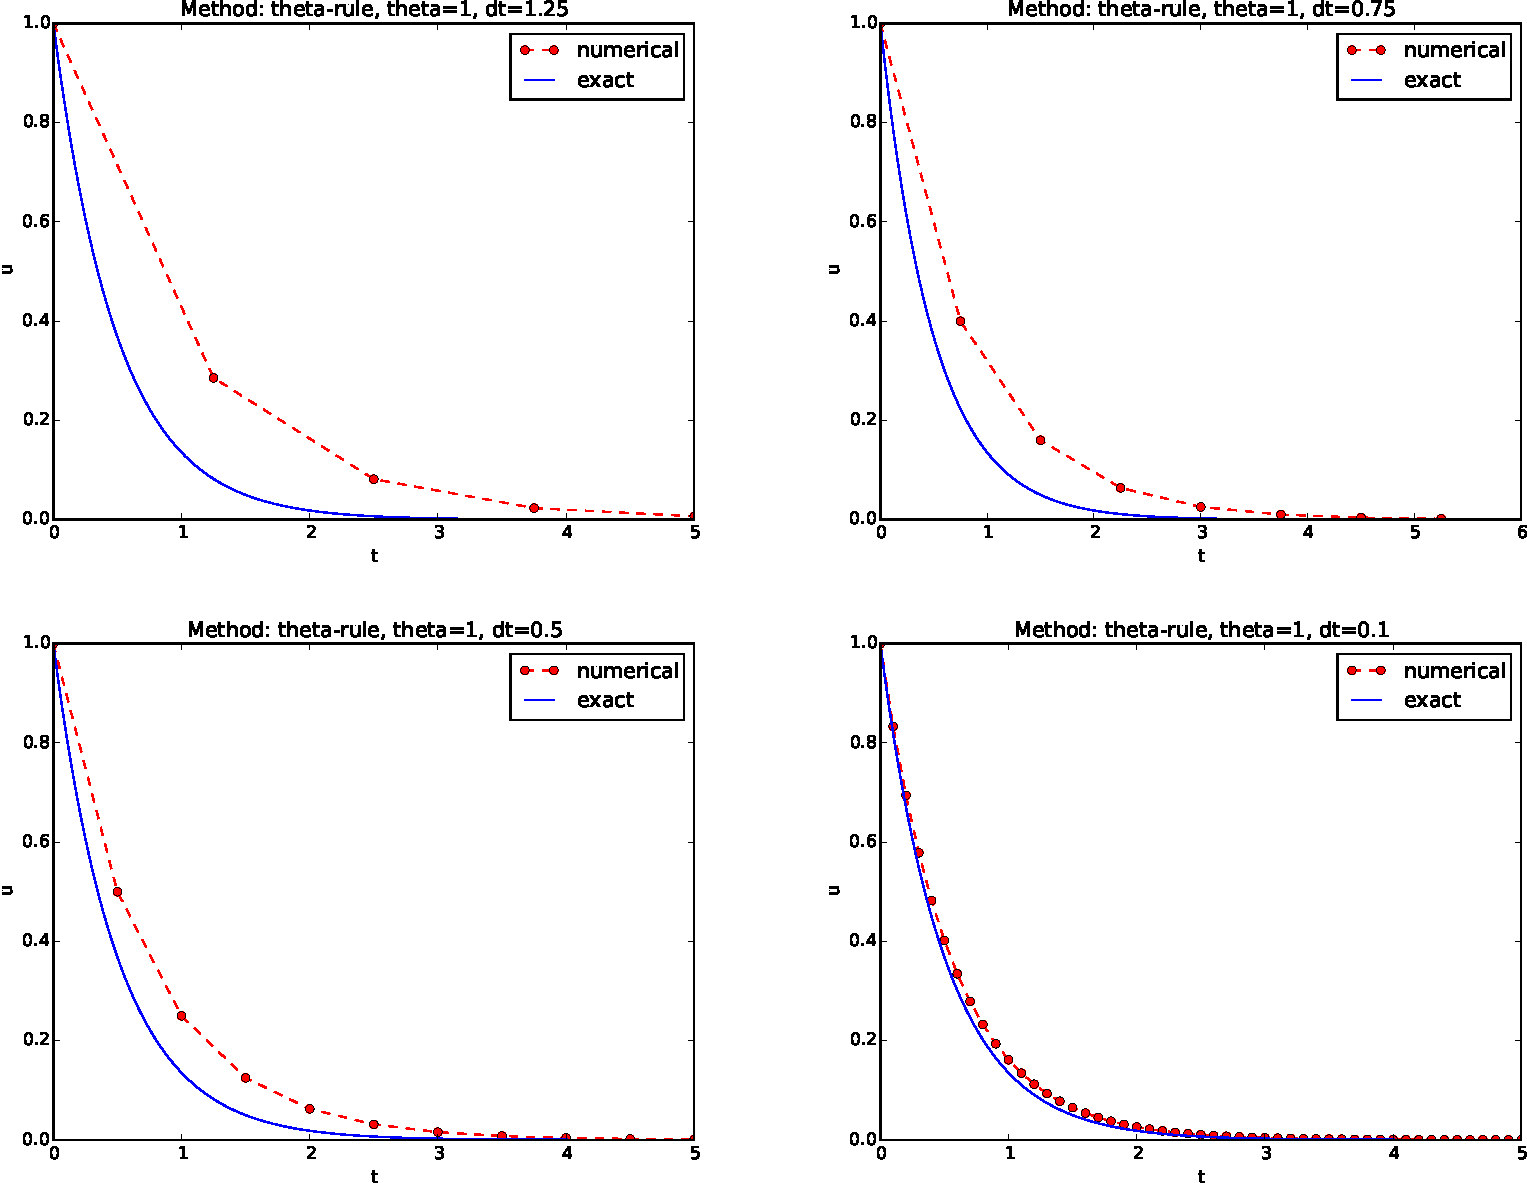
\includegraphics[width=1.1\linewidth]{fig-softeng/BE.pdf}}
  \caption{
  Illustration of the Backward Euler method for four time step values. \label{softeng1:experiments:fig:BE4a}
  }
\end{figure}
%\clearpage % flush figures softeng1:experiments:fig:BE4a


The appropriate ImageMagick commands are

\begin{Verbatim}[frame=lines,label=\fbox{{\tiny Terminal}},framesep=2.5mm,framerule=0.7pt,fontsize=\fontsize{9pt}{9pt}]
Terminal> montage -background white -geometry 100% -tile 2x \ 
          f1.png f2.png f3.png f4.png f.png
Terminal> convert -trim f.png f.png
Terminal> convert f.png -transparent white f.png
\end{Verbatim}
The first command mounts the four files in one, the next \texttt{convert} command
removes unnecessary surrounding white space, and the final \texttt{convert} command
makes the white background transparent.

High-quality montage of PDF files \texttt{f1.pdf},
\texttt{f2.pdf}, \texttt{f3.pdf}, and \texttt{f4.pdf} into \texttt{f.pdf} goes like

\begin{Verbatim}[frame=lines,label=\fbox{{\tiny Terminal}},framesep=2.5mm,framerule=0.7pt,fontsize=\fontsize{9pt}{9pt}]
Terminal> pdftk f1.pdf f2.pdf f3.pdf f4.pdf output tmp.pdf
Terminal> pdfnup --nup 2x2 --outfile tmp.pdf tmp.pdf
Terminal> pdfcrop tmp.pdf f.pdf
Terminal> rm -f tmp.pdf
\end{Verbatim}

\subsection{Running a program from Python}

The script for automating experiments needs to run the \texttt{model.py} program
with appropriate command-line options. Python has several tools for
executing an arbitrary command in the operating systems.
Let \texttt{cmd} be a string containing the desired command.
In the present case study, \texttt{cmd} could be \texttt{'python model.py --I 1 --dt 0.5 0.2'}.
The following code
executes \texttt{cmd} and loads the text output into a string \texttt{output}:

\begin{cod}{cbg_blue1}\begin{Verbatim}[numbers=none,fontsize=\fontsize{9pt}{9pt},baselinestretch=0.95,xleftmargin=2mm]
from subprocess import Popen, PIPE, STDOUT
p = Popen(cmd, shell=True, stdout=PIPE, stderr=STDOUT)
output, _ = p.communicate()

# Check if the execution was successful
failure = p.returncode
if failure:
    print 'Command failed:', cmd; sys.exit(1)
\end{Verbatim}
\end{cod}
\noindent
Unsuccessful execution usually makes it meaningless to continue
the program, and therefore we abort the program with \texttt{sys.exit(1)}.
Any argument different from 0 signifies to the computer's operating system
that our program stopped with a failure.


\begin{notice_mdfboxadmon}[Programming tip: use \protect\Verb!\_! for dummy variable]
Sometimes we need to unpack tuples or lists in separate variables,
but we are not interested in all the variables. One example is

\begin{cod}{cbg_blue1}\begin{Verbatim}[numbers=none,fontsize=\fontsize{9pt}{9pt},baselinestretch=0.95,xleftmargin=2mm]
output, error = p.communicate()
\end{Verbatim}
\end{cod}
\noindent
but \texttt{error} is of no interest in the example above.
One can then use underscore \Verb!_! as variable name for the dummy
(uninteresting) variable(s):

\begin{cod}{cbg_blue1}\begin{Verbatim}[numbers=none,fontsize=\fontsize{9pt}{9pt},baselinestretch=0.95,xleftmargin=2mm]
output, _ = p.communicate()
\end{Verbatim}
\end{cod}
\noindent
Here is another example where we iterate over a list of three-tuples,
but the interest is limited to the second element in each three-tuple:

\begin{cod}{cbg_blue1}\begin{Verbatim}[numbers=none,fontsize=\fontsize{9pt}{9pt},baselinestretch=0.95,xleftmargin=2mm]
for _, value, _ in list_of_three_tuples:
    # work with value
\end{Verbatim}
\end{cod}
\noindent
\end{notice_mdfboxadmon}



We need to interpret the contents of the string
\texttt{output} and store
the data in an appropriate data structure for further processing.
Since the content is basically a table and will be transformed to
a spread sheet format, we let the columns in the table be represented
by lists in the program,
and we collect these columns in a dictionary whose keys are natural
column names: \texttt{dt} and the three values of $\theta$.
The following code translates the output of \texttt{cmd} (\texttt{output})
to such a dictionary of lists (\texttt{errors}):

\begin{cod}{cbg_blue1}\begin{Verbatim}[numbers=none,fontsize=\fontsize{9pt}{9pt},baselinestretch=0.95,xleftmargin=2mm]
errors = {'dt': dt_values, 1: [], 0: [], 0.5: []}
for line in output.splitlines():
    words = line.split()
    if words[0] in ('0.0', '0.5', '1.0'):  # line with E?
        # typical line: 0.0   1.25:    7.463E+00
        theta = float(words[0])
        E = float(words[2])
        errors[theta].append(E)
\end{Verbatim}
\end{cod}
\noindent

\subsection{The automating script}

We have now all the core elements in place to write the complete
script where we run
\texttt{model.py} for a set of $\Delta t$ values (given as positional
command-line arguments), make the error plot,
write the CSV file, and combine plot files as described above.
The complete code is listed below, followed by some explaining comments.

\begin{pro}{cbg_blue1}{bar_blue1}\begin{Verbatim}[numbers=none,fontsize=\fontsize{9pt}{9pt},baselinestretch=0.95,xleftmargin=2mm]
import os, sys, glob
import matplotlib.pyplot as plt

def run_experiments(I=1, a=2, T=5):
    # The command line must contain dt values
    if len(sys.argv) > 1:
        dt_values = [float(arg) for arg in sys.argv[1:]]
    else:
        print 'Usage: %s dt1 dt2 dt3 ...' %  sys.argv[0]
        sys.exit(1)  # abort

    # Run module file and grab output
    cmd = 'python model.py --I %g --a %g --T %g' % (I, a, T)
    dt_values_str = ' '.join([str(v) for v in dt_values])
    cmd += ' --dt %s' % dt_values_str
    print cmd
    from subprocess import Popen, PIPE, STDOUT
    p = Popen(cmd, shell=True, stdout=PIPE, stderr=STDOUT)
    output, _ = p.communicate()
    failure = p.returncode
    if failure:
        print 'Command failed:', cmd; sys.exit(1)

    errors = {'dt': dt_values, 1: [], 0: [], 0.5: []}
    for line in output.splitlines():
        words = line.split()
        if words[0] in ('0.0', '0.5', '1.0'):  # line with E?
            # typical line: 0.0   1.25:    7.463E+00
            theta = float(words[0])
            E = float(words[2])
            errors[theta].append(E)

    # Find min/max for the axis
    E_min = 1E+20; E_max = -E_min
    for theta in 0, 0.5, 1:
        E_min = min(E_min, min(errors[theta]))
        E_max = max(E_max, max(errors[theta]))

    plt.loglog(errors['dt'], errors[0], 'ro-')
    plt.loglog(errors['dt'], errors[0.5], 'b+-')
    plt.loglog(errors['dt'], errors[1], 'gx-')
    plt.legend(['FE', 'CN', 'BE'], loc='upper left')
    plt.xlabel('log(time step)')
    plt.ylabel('log(error)')
    plt.axis([min(dt_values), max(dt_values), E_min, E_max])
    plt.title('Error vs time step')
    plt.savefig('error.png');  plt.savefig('error.pdf')

    # Write out a table in CSV format
    f = open('error.csv', 'w')
    f.write(r'$\Delta t$,$\theta=0$,$\theta=0.5$,$\theta=1$' + '\n')
    for _dt, _fe, _cn, _be in zip(
        errors['dt'], errors[0], errors[0.5], errors[1]):
        f.write('%.2f,%.4f,%.4f,%.4f\n' % (_dt, _fe, _cn, _be))
    f.close()

    # Combine images into rows with 2 plots in each row
    image_commands = []
    for method in 'BE', 'CN', 'FE':
        pdf_files = ' '.join(['%s_%g.pdf' % (method, dt)
                              for dt in dt_values])
        png_files = ' '.join(['%s_%g.png' % (method, dt)
                              for dt in dt_values])
        image_commands.append(
            'montage -background white -geometry 100%' +
            ' -tile 2x %s %s.png' % (png_files, method))
        image_commands.append(
            'convert -trim %s.png %s.png' % (method, method))
        image_commands.append(
            'convert %s.png -transparent white %s.png' %
            (method, method))
        image_commands.append(
            'pdftk %s output tmp.pdf' % pdf_files)
        num_rows = int(round(len(dt_values)/2.0))
        image_commands.append(
            'pdfnup --nup 2x%d --outfile tmp.pdf tmp.pdf' % num_rows)
        image_commands.append(
            'pdfcrop tmp.pdf %s.pdf' % method)

    for cmd in image_commands:
        print cmd
        failure = os.system(cmd)
        if failure:
            print 'Command failed:', cmd; sys.exit(1)

    # Remove the files generated above and by model.py
    from glob import glob
    filenames = glob('*_*.png') + glob('*_*.pdf') + glob('tmp*.pdf')
    for filename in filenames:
        os.remove(filename)

if __name__ == '__main__':
    run_experiments(I=1, a=2, T=5)
    plt.show()
\end{Verbatim}
\end{pro}
\noindent

\index{Unix wildcard notation} \index{wildcard notation (Unix)}
\index{os.system@{\rm\texttt{os.system}}}

We may comment upon many useful constructs in this script:

\begin{itemize}
 \item \texttt{[float(arg) for arg in sys.argv[1:]]} builds a list of real numbers
   from all the command-line arguments.

 \item \Verb!['%s_%s.png' % (method, dt) for dt in dt_values]! builds a list of
   filenames from a list of numbers (\Verb!dt_values!).

 \item All \texttt{montage}, \texttt{convert}, \texttt{pdftk}, \texttt{pdfnup}, and \texttt{pdfcrop}
   commands for creating
   composite figures are stored in a
   list and later executed in a loop.

 \item \Verb!glob('*_*.png')! returns a list of the names of all files in the
   current directory where the filename matches the \href{{http://en.wikipedia.org/wiki/Glob_(programming)}}{Unix wildcard notation}
   \Verb!*_*.png! (meaning any text, underscore, any text, and then \texttt{.png}).

 \item \texttt{os.remove(filename)} removes the file with name \texttt{filename}.

 \item \texttt{failure = os.system(cmd)} runs an operating system command with
   simpler syntax than what is required by \texttt{subprocess} (but the output
   of \texttt{cmd} cannot be captured).
\end{itemize}

\noindent
\subsection{Making a report}
\label{softeng1:exper:report}

The results of running computer experiments are best documented in a
little report containing the problem to be solved, key code segments,
and the plots from a series of experiments. At least the part of the
report containing the plots should be automatically generated by the
script that performs the set of experiments, because in the script we
know exactly which input data that were used to generate a specific
plot, thereby ensuring that each figure is connected to the
right data. Take a look at \href{{http://tinyurl.com/nc4upel/_static/sphinx-cloud/}}{a sample report}  to see what we have in
mind.

\index{Word (Microsoft)}
\index{LibreOffice}
\index{OpenOffice}
\index{Google Docs}

\paragraph{Word, OpenOffice, GoogleDocs.}
Microsoft Word, its open source counterparts OpenOffice and
LibreOffice, along with GoogleDocs and similar online services are the
dominating tools for writing reports today. Nevertheless, scientific
reports often need mathematical equations and nicely typeset computer
code in monospace font. The support for mathematics and computer code
in the mentioned tools is in this author's view not on par with the
technologies based on \emph{markup languages} and which are addressed
below. Also, with markup languages one has a readable, pure text file
as source for the report, and changes in this text can easily be
tracked by version control systems like Git. The result is a very
strong tool for monitoring ``who did what when'' with the files,
resulting in increased reliability of the writing process. For
collaborative writing, the merge functionality in Git leads to safer
simultaneously editing than what is offered even by collaborative
tools like GoogleDocs.



\index{HTML}
\index{MathJax}

\paragraph{HTML with MathJax.}
HTML is the markup language used for web pages.  Nicely typeset computer
code is straightforward in HTML, and high-quality mathematical
typesetting is available using an extension to HTML called \href{{http://www.mathjax.org/}}{MathJax}, which allows formulas and equations to be
typeset with {\LaTeX} syntax and nicely rendered in web browsers, see
Figure~\ref{softeng1:exper:report:fig:mathjax}.  A relatively small
subset of {\LaTeX} environments for mathematics is supported, but the
syntax for formulas is quite rich. Inline formulas look like \Verb!\( u'=-au \)! while equations are surrounded by \Verb!$$! signs.  Inside such
signs, one can use \Verb!\[ u'=-au \]! for unnumbered equations, or
\Verb!\begin{equation}! and \Verb!\end{equation}! for
numbered equations, or \Verb!\begin{align}! and \Verb!\end{align}! for multiple
numbered aligned equations.  You need to be familiar with \href{{http://en.wikibooks.org/wiki/LaTeX/Mathematics}}{mathematical
typesetting in LaTeX} to write MathJax
code.

The file \href{{http://tinyurl.com/p96acy2/report_generation/exper1_html.py}}{\nolinkurl{exper1_mathjax.py}}
calls a script
\href{{http://tinyurl.com/p96acy2/exper1.py}}{\nolinkurl{exper1.py}}
to perform the numerical experiments and then runs Python
statements for creating an \href{{http://tinyurl.com/nc4upel/_static/report_mathjax.html.html}}{HTML file} with the source code for \href{{http://tinyurl.com/nc4upel/_static/report_mathjax.html}}{the scientific report}.


\begin{figure}[!ht]  % softeng1:exper:report:fig:mathjax
  \centerline{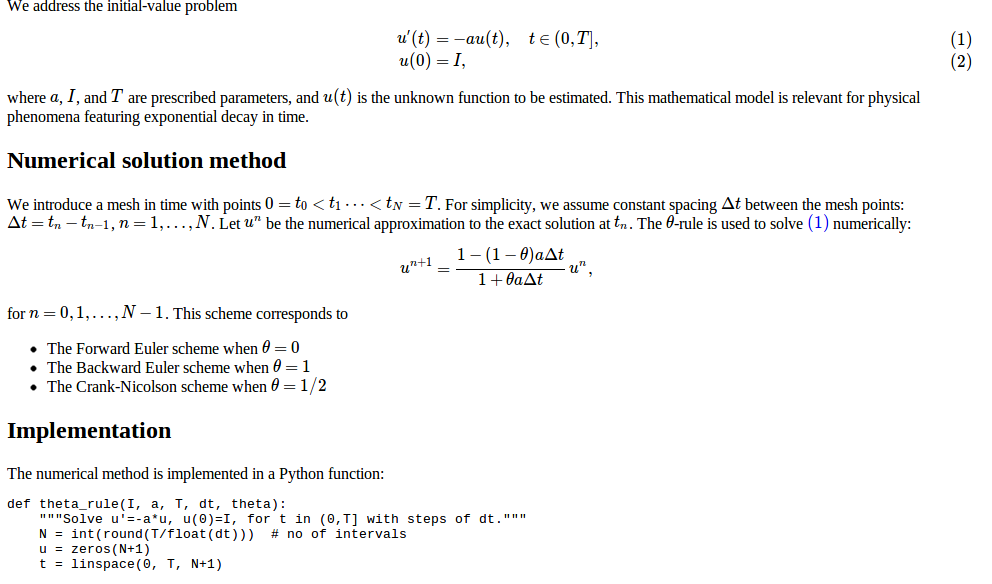
\includegraphics[width=0.9\linewidth]{fig-softeng/report_mathjax.png}}
  \caption{
  Report in HTML format with MathJax. \label{softeng1:exper:report:fig:mathjax}
  }
\end{figure}
%\clearpage % flush figures softeng1:exper:report:fig:mathjax


\index{LaTeX}

\paragraph{{\LaTeX}.}
% "http://en.wikibooks.org/wiki/LaTeX"

The \emph{de facto} language for mathematical typesetting and scientific
report writing is \href{{http://en.wikipedia.org/wiki/LaTeX}}{LaTeX}. A
number of very sophisticated packages have been added to the language
over a period of three decades, allowing very fine-tuned layout and
typesetting. For output in the \href{{http://tinyurl.com/nc4upel/_static/report.pdf}}{PDF format}, see Figure~\ref{softeng1:exper:report:fig:latex} for an example, {\LaTeX} is the
definite choice when it comes to \emph{typesetting quality}.
The {\LaTeX} language used to
write the reports has typically a lot of commands involving
\href{{http://tinyurl.com/nc4upel/_static/report.tex.html}}{backslashes and braces}, and many claim that
{\LaTeX} syntax is not particularly readable.  For output on the web via
HTML code (i.e., not only showing the PDF in the browser window), {\LaTeX}
struggles with delivering high quality typesetting. Other tools,
especially Sphinx, give better results and can also produce
nice-looking PDFs.  The file \href{{http://tinyurl.com/p96acy2/report_generation/exper1_latex.py}}{\nolinkurl{exper1_latex.py}} shows how to
generate the {\LaTeX} source from a program.


\begin{figure}[!ht]  % softeng1:exper:report:fig:latex
  \centerline{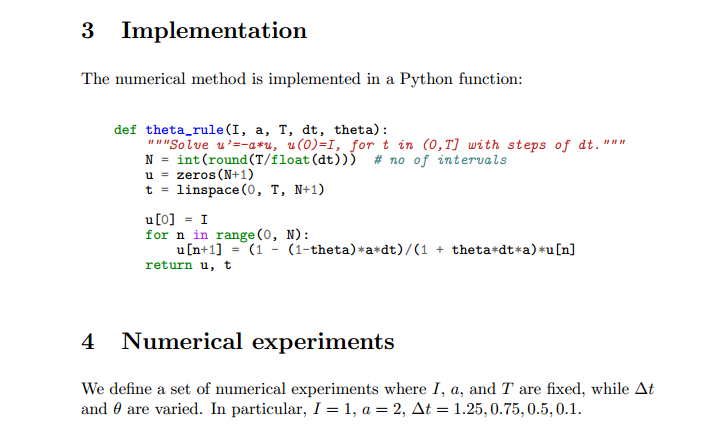
\includegraphics[width=0.9\linewidth]{fig-softeng/report_latexpdf.png}}
  \caption{
  Report in PDF format generated from {\LaTeX} source. \label{softeng1:exper:report:fig:latex}
  }
\end{figure}
%\clearpage % flush figures softeng1:exper:report:fig:latex


\index{Sphinx (typesetting tool)}

\paragraph{Sphinx.}
% give pointers to source pages

\href{{http://sphinx.pocoo.org/}}{Sphinx} is a typesetting language with
similarities to HTML and {\LaTeX}, but with much less tagging. It has
recently become very popular for software documentation and
mathematical reports. Sphinx can utilize {\LaTeX} for mathematical
formulas and equations. Unfortunately, the
subset of {\LaTeX} mathematics supported is less than in full MathJax (in
particular, numbering of multiple equations in an \texttt{align} type
environment is not supported).  The \href{{http://tinyurl.com/nc4upel/_static/report_sphinx.rst.html}}{Sphinx syntax} is an extension of
the reStructuredText language. An attractive feature of Sphinx is its
rich support for \href{{http://tinyurl.com/nc4upel/_static/sphinx-cloud/index.html}}{fancy layout of web pages}. In particular,
Sphinx can easily be combined with various layout \emph{themes} that give a
certain look and feel to the web site and that offers table of
contents, navigation, and search facilities, see Figure~\ref{softeng1:exper:report:fig:sphinx}.


\begin{figure}[!ht]  % softeng1:exper:report:fig:sphinx
  \centerline{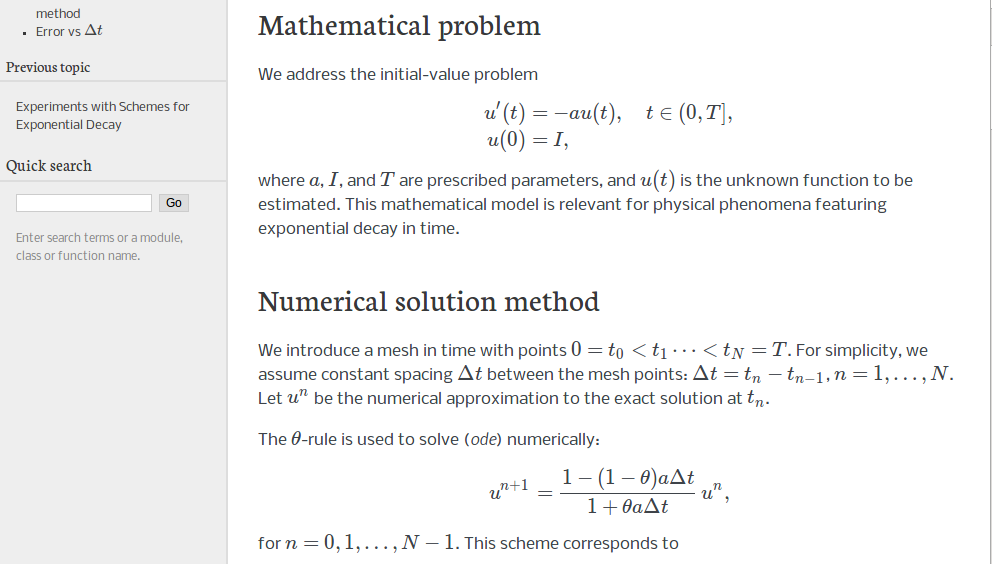
\includegraphics[width=0.9\linewidth]{fig-softeng/report_sphinx.png}}
  \caption{
  Report in HTML format generated from Sphinx source. \label{softeng1:exper:report:fig:sphinx}
  }
\end{figure}
%\clearpage % flush figures softeng1:exper:report:fig:sphinx


\index{Markdown}

\paragraph{Markdown.}
A recent, very popular format for easy writing of web pages is
\href{{http://daringfireball.net/projects/markdown/}}{Markdown}.
Text is written very much like one would do in email, using
spacing and special characters to naturally format the code
instead of heavily tagging the text as in {\LaTeX} and HTML.
With the tool \href{{http://johnmacfarlane.net/pandoc/}}{Pandoc} one
can go from Markdown to a variety of formats.
HTML is a common output format, but {\LaTeX}, epub, XML,
OpenOffice/LibreOffice, MediaWiki, and Microsoft Word are some other
possibilities. A Markdown version of our scientific
report demo is available as an IPython/Jupyter notebook (described next).

\index{IPython notebooks}
\index{Jupyter notebooks}

\paragraph{IPython/Jupyter notebooks.}
The \href{{http://ipython.org/notebook.html}}{IPython Notebook} is
a web-based tool where one can write scientific reports with live computer
code and graphics. Or the other way around: software can be equipped
with documentation in the style of scientific reports.
A slightly extended version of Markdown is used for writing text and
mathematics, and the \href{{http://tinyurl.com/nc4upel/_static/report.ipynb.html}}{source code of a notebook} is in json format.
The interest in the notebook has grown amazingly fast
over just a few years, and further development now takes place
in the \href{{https://jupyter.org/}}{Jupyter project}, which
supports a lot of programming languages for interactive notebook computing.
Jupyter notebooks are primarily live electronic documents, but they can be
printed out as PDF reports too.
A notebook version of our scientific report can be \href{{http://tinyurl.com/p96acy2/_static/report.ipynb}}{downloaded} and experimented with
or \href{{http://nbviewer.ipython.org/url/hplgit.github.com/teamods/writing_reports/_static/report.ipynb}}{just statically viewed} in a browser.

\paragraph{Wiki formats.}
A range of wiki formats are popular for creating notes on the web,
especially documents which allow groups of people to edit and add
content. Apart from \href{{http://www.mediawiki.org/wiki/MediaWiki}}{MediaWiki} (the wiki format used for
Wikipedia), wiki formats have no support for mathematical typesetting
and also limited tools for displaying computer code in nice ways.
Wiki formats are therefore less suitable for scientific reports compared
to the other formats mentioned here.

\index{DocOnce}

\paragraph{DocOnce.}
Since it is difficult to choose the right tool or format for writing a
scientific report, it is advantageous to write the content in a format
that easily translates to {\LaTeX}, HTML, Sphinx, Markdown,
IPython/Jupyter notebooks, and various wikis. \href{{https://github.com/hplgit/doconce}}{DocOnce} is such a tool. It is similar to
Pandoc, but offers some special convenient features for writing about
mathematics and programming.  The \href{{http://tinyurl.com/nc4upel/_static/report.do.txt.html}}{tagging is modest}, somewhere between
{\LaTeX} and Markdown.  The program \href{{http://tinyurl.com/p96acy2/exper1_do.py}}{\nolinkurl{exper1_do.py}} demonstrates how
to generate DocOnce code for a scientific report.
There is also a corresponding rich demo of the \href{{http://tinyurl.com/nc4upel/index.html}}{resulting reports} that can be made from
this DocOnce code.


% project with exploring instability (help with matplotlib contour plots, and maybe show such a plot)

\subsection{Publishing a complete project}
\label{softeng1:exper:github}

\index{replicability}

To assist the important principle of \emph{replicable} science,
a report documenting scientific investigations should be accompanied by
all the software and data used for the investigations so that others
have a possibility to redo the work and assess the qualify of the results.

One way of documenting a complete project is to make a directory tree
with all relevant files. Preferably, the tree is published at
some project hosting site like \href{{http://hplgit.github.com/teamods/bitgit/html/}}{Bitbucket or GitHub} so that others can download it
as a tarfile, zipfile, or clone the files directly using the Git version control
system.
For the investigations outlined in Section~\ref{softeng1:exper:report},
we can create a directory tree with files
\begin{cod}{cbg_blue1}\begin{Verbatim}[numbers=none,fontsize=\fontsize{9pt}{9pt},baselinestretch=0.95,xleftmargin=2mm]
setup.py
./src:
   model.py
./doc:
   ./src:
      exper1_mathjax.py
      make_report.sh
      run.sh
   ./pub:
      report.html
\end{Verbatim}
\end{cod}
\noindent
The \texttt{src} directory holds source code (modules) to be reused in other projects,
the \texttt{setup.py} script builds and installs such software,
the \texttt{doc} directory contains the documentation, with \texttt{src} for the
source of the documentation (usually written in a markup language)
and \texttt{pub} for published (compiled) documentation.
The \texttt{run.sh} file is a simple Bash script listing the \texttt{python} commands
we used to run \Verb!exper1_mathjax.py! to generate the experiments and
the \texttt{report.html} file.

% Point to DocOnce version


\section{Exercises}



% --- begin exercise ---
\begin{doconceexercise}
\refstepcounter{doconceexercisecounter}

\subsection*{Problem \thedoconceexercisecounter: Make a tool for differentiating curves}
\addcontentsline{loe}{doconceexercise}{Problem \thedoconceexercisecounter: Make a tool for differentiating curves}

\label{softeng1:exer:derivative}

Suppose we have a curve specified through a set
of discrete coordinates $(x_i,y_i)$, $i=0,\ldots,n$, where the $x_i$
values are uniformly distributed with spacing $\Delta x$: $x_i=\Delta x$.
The derivative of this curve, defined as a new curve with points
$(x_i, d_i)$, can be computed via finite differences:

\begin{align}
d_0 &= \frac{y_1-y_0}{\Delta x},\\ 
d_i &= \frac{y_{i+1}-y_{i-1}}{2\Delta x},\quad i=1,\ldots,n-1,\\ 
d_n &= \frac{y_n-y_{n-1}}{\Delta x}\tp
\end{align}


\subex{a)}
Write a function
\texttt{differentiate(x, y)} for differentiating a curve
with coordinates in the arrays \texttt{x} and \texttt{y}, using the
formulas above. The function should return the coordinate arrays
of the resulting differentiated curve.

\subex{b)}
Since the formulas for differentiation used here are only approximate,
with unknown approximation errors, it is challenging to construct
test cases. Here are three approaches, which should be implemented
in three separate test functions.

\begin{enumerate}
\item Consider a curve with three points and compute $d_i$, $i=0,1,2$,
   by hand. Make a test that compares the hand-calculated results with those
   from the function in a).

\item The formulas for $d_i$ are exact for points on
   a straight line, as all the $d_i$ values are then the same, equal to
   the slope of the line. A test can check this property.

\item For points lying on a parabola, the values for $d_i$, $i=1,\ldots,n-1$,
   should equal the exact derivative of the parabola. Make a test based on
   this property.
\end{enumerate}

\noindent
\subex{c)}
Start with a curve corresponding to $y=\sin(\pi x)$ and $n+1$
points in $[0,1]$. Apply \texttt{differentiate} four times and plot the
resulting curve and the exact $y=\sin\pi x$ for $n=6, 11, 21, 41$.

% Using a 2nd-order backward formula at x=1 does not improve the
% results much, one gets large errors at the end points.


\noindent Filename: \texttt{curvediff}.

\end{doconceexercise}
% --- end exercise ---




% --- begin exercise ---
\begin{doconceexercise}
\refstepcounter{doconceexercisecounter}

\subsection*{Problem \thedoconceexercisecounter: Make solid software for the Trapezoidal rule}
\addcontentsline{loe}{doconceexercise}{Problem \thedoconceexercisecounter: Make solid software for the Trapezoidal rule}

\label{softeng1:exer:integral:flat}

An integral

\[ \int_a^b f(x)dx \]
can be numerically approximated by the Trapezoidal rule,

\[ \int_a^b f(x)dx \approx \frac{h}{2}(f(a) + f(b)) + h\sum_{i=1}^{n-1} f(x_i),
\]
where $x_i$ is a set of uniformly spaced points in $[a,b]$:

\[ h = \frac{b-a}{n},\quad x_i=a + ih,\ i=1,\ldots,n-1\tp \]

Somebody has used this rule to compute the integral $\int_0^\pi \sin^2x\, dx$:

\begin{pro}{cbg_blue1}{bar_blue1}\begin{Verbatim}[numbers=none,fontsize=\fontsize{9pt}{9pt},baselinestretch=0.95,xleftmargin=2mm]
from math import pi, sin
np = 20
h = pi/np
I = 0
for k in range(1, np):
    I += sin(k*h)**2
print I
\end{Verbatim}
\end{pro}
\noindent


\subex{a)}
The ``flat'' implementation above suffers from serious flaws:

\begin{enumerate}
\item A general numerical algorithm (the Trapezoidal rule) is implemented
   in a specialized form where the formula for $f$ is inserted directly
   into the code for the general integration formula.

\item A general numerical algorithm is not encapsulated as a general
   function, with appropriate parameters, which can be reused
   across a wide range of applications.

\item The lazy programmer dropped the first terms in the general formula
   since $\sin(0)=\sin(\pi)=0$.

\item The sloppy programmer used \texttt{np} (number of points?) as variable for
   \texttt{n} in the formula and a counter \texttt{k} instead of \texttt{i}. Such small
   deviations from the mathematical notation are completely unnecessary.
   The closer the code and the mathematics can get, the easier it is
   to spot errors in formulas.
\end{enumerate}

\noindent
Write a function \texttt{trapezoidal} that fixes these flaws.
Place the function in a module \texttt{trapezoidal}.

\subex{b)}
Write a test function \Verb!test_trapezoidal!. Call the test function
explicitly to check that it works. Remove the call and run pytest
on the module:

\begin{Verbatim}[frame=lines,label=\fbox{{\tiny Terminal}},framesep=2.5mm,framerule=0.7pt,fontsize=\fontsize{9pt}{9pt}]
Terminal> py.test -s -v trapezoidal
\end{Verbatim}

% --- begin hint in exercise ---

\paragraph{Hint.}
Note that even if you know the value of the integral, you do not know
the error in the approximation produced by the Trapezoidal rule.
However, the Trapezoidal rule will integrate linear functions
exactly (i.e., to machine precision). Base a test function
on a linear $f(x)$.

% --- end hint in exercise ---

\subex{c)}
Add functionality such that we can compute $\int_a^b f(x)dx$ by providing
$f$, $a$, $b$, and $n$ as positional command-line arguments to the
module file:

\begin{Verbatim}[frame=lines,label=\fbox{{\tiny Terminal}},framesep=2.5mm,framerule=0.7pt,fontsize=\fontsize{9pt}{9pt}]
Terminal> python trapezoidal.py 'sin(x)**2' 0 pi 20
\end{Verbatim}
Here, $a=0$, $b=\pi$, and $n=20$.

Note that the \texttt{trapezoidal.py} file must still be a valid module file, so the
interpretation of command-line data and computation of the integral
must be performed from calls in a test block.

% --- begin hint in exercise ---

\paragraph{Hint.}
To translate a string formula on the command line, like \texttt{sin(x)**2},
into a Python function, you can wrap a function declaration around
the formula and run \texttt{exec} on the string to turn it into live Python code:

\begin{cod}{cbg_blue1}\begin{Verbatim}[numbers=none,fontsize=\fontsize{9pt}{9pt},baselinestretch=0.95,xleftmargin=2mm]
import math, sys
formula = sys.argv[1]
f_code = """
def f(x):
    return %s
""" % formula
exec(code, math.__dict__)
\end{Verbatim}
\end{cod}
\noindent
The result is the same as if we had hardcoded

\begin{cod}{cbg_blue1}\begin{Verbatim}[numbers=none,fontsize=\fontsize{9pt}{9pt},baselinestretch=0.95,xleftmargin=2mm]
from math import *

def f(x):
    return sin(x)**2
\end{Verbatim}
\end{cod}
\noindent
in the program. Note that \texttt{exec} needs the namespace
\Verb!math.__dict__!, i.e., all names in the \texttt{math} module, such that
it understands \texttt{sin} and other mathematical functions.
Similarly, to allow $a$ and $b$ to be \texttt{math} expressions like \texttt{pi/4}
and \texttt{exp(4)}, do

\begin{Verbatim}[frame=lines,label=\fbox{{\tiny Terminal}},framesep=2.5mm,framerule=0.7pt,fontsize=\fontsize{9pt}{9pt}]
a = eval(sys.argv[2], math.__dict__)
b = eval(sys.argv[2], math.__dict__)
\end{Verbatim}

% --- end hint in exercise ---

\subex{d)}
Write a test function for verifying the implementation of
data reading from the command line.

\noindent Filename: \texttt{trapezoidal}.

\end{doconceexercise}
% --- end exercise ---




% --- begin exercise ---
\begin{doconceexercise}
\refstepcounter{doconceexercisecounter}

\subsection*{Problem \thedoconceexercisecounter: Implement classes for the Trapezoidal rule}
\addcontentsline{loe}{doconceexercise}{Problem \thedoconceexercisecounter: Implement classes for the Trapezoidal rule}

\label{softeng1:exer:integral:flat2}

We consider the same problem setting as in Problem~\ref{softeng1:exer:integral:flat}. Make a module with a class \texttt{Problem}
representing the mathematical problem to be solved and a class
\texttt{Solver} representing the solution method.  The rest of the
functionality of the module, including test functions and reading data
from the command line, should be as in Problem~\ref{softeng1:exer:integral:flat}.
\noindent Filename: \Verb!trapezoidal_class!.

\end{doconceexercise}
% --- end exercise ---




% --- begin exercise ---
\begin{doconceexercise}
\refstepcounter{doconceexercisecounter}

\subsection*{Problem \thedoconceexercisecounter: Write a doctest and a test function}
\addcontentsline{loe}{doconceexercise}{Problem \thedoconceexercisecounter: Write a doctest and a test function}

\label{softeng1:exer:doctest1}

Type in the following program:

\begin{pro}{cbg_blue1}{bar_blue1}\begin{Verbatim}[numbers=none,fontsize=\fontsize{9pt}{9pt},baselinestretch=0.95,xleftmargin=2mm]
import sys
# This sqrt(x) returns real if x>0 and complex if x<0
from numpy.lib.scimath import sqrt

def roots(a, b, c):
    """
    Return the roots of the quadratic polynomial
    p(x) = a*x**2 + b*x + c.

    The roots are real or complex objects.
    """
    q = b**2 - 4*a*c
    r1 = (-b + sqrt(q))/(2*a)
    r2 = (-b - sqrt(q))/(2*a)
    return r1, r2

a, b, c = [float(arg) for arg in sys.argv[1:]]
print roots(a, b, c)
\end{Verbatim}
\end{pro}
\noindent


\subex{a)}
Equip the \texttt{roots} function with a doctest.
Make sure to test both real and complex roots.
Write out numbers in the doctest with 14 digits or less.

\subex{b)}
Make a test function for the \texttt{roots} function. Perform the
same mathematical tests as in a), but with different
programming technology.

\noindent Filename: \Verb!test_roots!.

\end{doconceexercise}
% --- end exercise ---




% --- begin exercise ---
\begin{doconceexercise}
\refstepcounter{doconceexercisecounter}

\subsection*{Problem \thedoconceexercisecounter: Experiment with tolerances in comparisons}
\addcontentsline{loe}{doconceexercise}{Problem \thedoconceexercisecounter: Experiment with tolerances in comparisons}

\label{softeng1:exer:tol}

When we replace a comparison \texttt{a == b}, where \texttt{a} and/or \texttt{b} are
\texttt{float} objects, by a comparison with tolerance, \texttt{abs(a-b) < tol},
the appropriate size of \texttt{tol} depends on the size of \texttt{a} and \texttt{b}.
Investigate how the size of \texttt{abs(a-b)} varies when \texttt{b} takes on
values $10^k$, $k=-5,-9,\ldots,20$ and \texttt{a=1.0/49*b*49}.
\noindent Filename: \texttt{tolerance}.

% Closing remarks for this Problem

\paragraph{Remarks.}
You will experience that if \texttt{a} and \texttt{b} are large, as they can be
in geophysical applications where lengths measured in meters can be of size
$10^6$ m, \texttt{tol} must be about $10^{-9}$, while \texttt{a} and \texttt{b} around unity can
have \texttt{tol} of size $10^{-15}$.


\end{doconceexercise}
% --- end exercise ---




% --- begin exercise ---
\begin{doconceexercise}
\refstepcounter{doconceexercisecounter}

\subsection*{Exercise \thedoconceexercisecounter: Make use of a class implementation}
\addcontentsline{loe}{doconceexercise}{Exercise \thedoconceexercisecounter: Make use of a class implementation}

\label{softeng1:exer:class:dts}

Implement the \Verb!experiment_compare_dt! function from \texttt{decay.py}
using class \texttt{Problem} and class \texttt{Solver} from
Section~\ref{softeng1:prog:se:class}.
The parameters \texttt{I}, \texttt{a}, \texttt{T}, the scheme name, and a series of
\texttt{dt} values should be read from the command line.
\noindent Filename: \Verb!experiment_compare_dt_class!.

\end{doconceexercise}
% --- end exercise ---




% --- begin exercise ---
\begin{doconceexercise}
\refstepcounter{doconceexercisecounter}

\subsection*{Problem \thedoconceexercisecounter: Make solid software for a difference equation}
\addcontentsline{loe}{doconceexercise}{Problem \thedoconceexercisecounter: Make solid software for a difference equation}

\label{softeng1:exer:logistic}

We have the following evolutionary difference equation for the number
of individuals $u^n$ of a certain specie at time $n\Delta t$:

\begin{equation}
u^{n+1} = u^n + \Delta t\, r u^n\left(1 - \frac{u^n}{M^n}\right),
\quad u^0=U_0\tp
\label{softeng1:exer:logistic:eq}
\end{equation}
Here, $n$ is a counter in time, $\Delta t$ is time between time levels
$n$ and $n+1$ (assumed constant), $r$ is a net reproduction rate
for the specie,
and $M^n$ is the upper limit of the population that the environment can
sustain at time level $n$.
\noindent Filename: \texttt{logistic}.

\end{doconceexercise}
% --- end exercise ---


% !split

\clearemptydoublepage
\markboth{Bibliography}{Bibliography}
\thispagestyle{empty}

\bibliographystyle{plain}
\bibliography{../chapters/papers}

% ------------------- end of main content ---------------

% #ifdef PREAMBLE
\cleardoublepage\phantomsection  % trick to get correct link to Index
\printindex

\end{document}
% #endif

